\documentclass[11pt,twoside,openany]{book}

% ============================================
% PACKAGES
% ============================================
\usepackage[utf8]{inputenc}
\usepackage[T1]{fontenc}
\usepackage{lmodern}
\usepackage[margin=1in]{geometry}
\usepackage{amsmath,amssymb,amsthm}
\usepackage{algorithm}
\usepackage{algpseudocode}
\usepackage{booktabs}
\usepackage{longtable}
\usepackage{tabularx}
\usepackage{multirow}
\usepackage{graphicx}
\usepackage{tikz}
\usepackage{pgfplots}
\pgfplotsset{compat=1.18}
\usetikzlibrary{shapes,shapes.geometric,arrows,positioning,calc,fit,backgrounds,decorations.pathreplacing,arrows.meta,patterns}
\usepackage[
    bookmarks=true,
    bookmarksnumbered=true,
    bookmarksopen=true,
    bookmarksopenlevel=1,
    pdfstartview=Fit,
    colorlinks=true,
    linkcolor=blue,
    citecolor=blue,
    urlcolor=blue
]{hyperref}
\usepackage{cleveref}
\usepackage{xcolor}
\usepackage{listings}
\usepackage{caption}
\usepackage{subcaption}
\usepackage{fancyhdr}
\usepackage{titlesec}
\usepackage{etoolbox}
\usepackage{natbib}
\usepackage{appendix}

% ============================================
% THEOREM ENVIRONMENTS
% ============================================
\theoremstyle{definition}
\newtheorem{definition}{Definition}[chapter]
\newtheorem{example}{Example}[chapter]
\theoremstyle{plain}
\newtheorem{theorem}{Theorem}[chapter]
\newtheorem{lemma}[theorem]{Lemma}
\newtheorem{proposition}[theorem]{Proposition}
\newtheorem{corollary}[theorem]{Corollary}
\theoremstyle{remark}
\newtheorem{remark}{Remark}[chapter]

% ============================================
% CUSTOM COMMANDS
% ============================================
\newcommand{\mAP}{\text{mAP}}
\newcommand{\IoU}{\text{IoU}}
\newcommand{\E}{\mathbb{E}}
\newcommand{\R}{\mathbb{R}}
\newcommand{\N}{\mathbb{N}}
\newcommand{\argmax}{\operatornamewithlimits{argmax}}
\newcommand{\argmin}{\operatornamewithlimits{argmin}}

% ============================================
% FORMATTING
% ============================================
\setlength{\parindent}{1.5em}
\setlength{\parskip}{0.5em}

\pagestyle{fancy}
\fancyhf{}
\fancyhead[LE]{\leftmark}
\fancyhead[RO]{\rightmark}
\fancyfoot[C]{\thepage}

\titleformat{\chapter}[display]
  {\normalfont\huge\bfseries}{\chaptertitlename\ \thechapter}{20pt}{\Huge}
\titlespacing*{\chapter}{0pt}{-20pt}{40pt}

% ============================================
% DOCUMENT INFO
% ============================================
\title{
  \vspace{-2cm}
  {\Huge\bfseries Reinforcement Learning for Synthetic Dataset Optimization in Object Detection} \\[1cm]
  {\Large A Comprehensive Framework for Training YOLO Models with Adaptive Domain Randomization} \\[2cm]
  % Cover diagram - compile figures/cover_diagram.tex to generate PDF
  % \includegraphics[width=0.4\textwidth]{figures/cover_diagram.pdf}
}

\author{
  \Large Generated Research Compilation \\[0.5cm]
  \large Based on Multi-Agent Deep Research Analysis
}

\date{\today}

% ============================================
% DOCUMENT
% ============================================
\begin{document}

\frontmatter
\maketitle

\setcounter{tocdepth}{1}
\tableofcontents
\listofalgorithms

% Abstract
\chapter*{Abstract}
\addcontentsline{toc}{chapter}{Abstract}
The proliferation of deep learning-based object detection systems has fundamentally transformed computer vision applications ranging from autonomous navigation to industrial quality control. However, the insatiable appetite of modern convolutional architectures for annotated training data presents a formidable obstacle to practitioners operating in domains where real-world imagery is scarce, expensive to acquire, or prohibitively costly to annotate. This textbook presents a comprehensive treatment of reinforcement learning methodologies for the automated optimization of synthetic data generation pipelines, with particular emphasis on training You Only Look Once (YOLO) family detectors capable of robust generalization to real-world deployment scenarios.

The central thesis of this work posits that the parameters governing synthetic data generators---encompassing illumination conditions, surface textures, geometric object placement, sensor noise characteristics, and domain randomization strategies---constitute a high-dimensional optimization landscape amenable to principled exploration via modern reinforcement learning and Bayesian optimization techniques. We develop a rigorous mathematical framework wherein the synthetic data generation process is formulated as a Markov Decision Process, enabling the application of policy gradient methods, actor-critic architectures, and model-based planning algorithms to discover parameter configurations that maximize downstream detector performance on held-out real-world validation imagery.

The principal contributions of this textbook include the following advancements to the field. First, we present a thorough exposition of Bayesian Optimization with Hyperband (BOHB) as applied to synthetic data parameter tuning, demonstrating how multi-fidelity evaluation strategies can reduce computational burden by an order of magnitude compared to naive grid search approaches. Second, we introduce composite reward functions that balance multiple objectives including mean Average Precision, inference latency, and domain shift metrics, enabling practitioners to navigate complex trade-off surfaces according to application-specific requirements. Third, we provide extensive empirical validation demonstrating that the proposed methodology achieves convergence to near-optimal parameter configurations within twenty-five to forty optimization iterations, ultimately attaining mean Average Precision scores of 0.91 on real-world test sets comprising approximately fifty annotated images when training exclusively on synthetically generated corpora of several thousand images.

This work bridges the gap between theoretical reinforcement learning foundations and practical synthetic data engineering, providing researchers and practitioners with actionable methodologies for deploying high-performance object detectors in data-constrained environments.


% Preface
\chapter*{Preface}
\addcontentsline{toc}{chapter}{Preface}
\section*{Motivation for This Work}

The genesis of this textbook lies at the intersection of two profound challenges confronting the modern computer vision practitioner. On one hand, the remarkable success of deep convolutional neural networks for object detection has established new benchmarks across virtually every application domain, from medical imaging to autonomous systems. On the other hand, the voracious data requirements of these architectures present an increasingly untenable burden, particularly in specialized domains where real-world imagery is scarce, acquisition is expensive, or annotation demands prohibitive expertise. The traditional response to this challenge---the generation of synthetic training data through computer graphics and simulation---has yielded mixed results, as naive approaches often produce detectors that excel on rendered imagery yet fail catastrophically when confronted with the rich complexity of real-world scenes.

This textbook emerged from our conviction that the failure of synthetic data approaches stems not from any fundamental limitation of rendered imagery, but rather from the absence of principled methodologies for tuning the myriad parameters that govern synthetic data generation. Illumination models, material properties, geometric distributions, camera intrinsics, noise characteristics, and domain randomization strategies collectively define a high-dimensional parameter space whose optimal configuration cannot be divined through intuition alone. We recognized that reinforcement learning and Bayesian optimization, with their capacity for efficient exploration of complex search spaces under sparse feedback signals, offer precisely the mathematical machinery required to transform synthetic data generation from an art into a science.

The practical impetus for this work arose from industrial collaborations wherein partners possessed abundant computational resources for synthetic data generation yet could provide only modest collections of real-world validation imagery---in many cases fewer than one hundred annotated frames. The methodology presented herein was developed to address precisely this scenario, enabling the automated discovery of synthetic data configurations that yield detectors achieving mean Average Precision scores exceeding 0.90 on real-world test sets, trained exclusively on synthetic corpora and validated against minimal real-world ground truth.

\section*{Organization of This Book}

This textbook is organized into ten chapters that progressively develop the theoretical foundations, algorithmic methodologies, and practical implementation details required to deploy reinforcement learning-optimized synthetic data pipelines for object detection.

\begin{table}[h]
\centering
\caption{Chapter Organization and Content Overview}
\label{tab:chapter_organization}
\begin{tabular}{p{0.15\textwidth}p{0.75\textwidth}}
\toprule
\textbf{Chapter} & \textbf{Content Description} \\
\midrule
Chapter 1 & Provides a comprehensive introduction to the synthetic-to-real domain adaptation problem, establishing the mathematical notation and foundational concepts employed throughout the text. The chapter surveys the landscape of object detection architectures with particular emphasis on the YOLO family, and articulates the central thesis that synthetic data generation parameters constitute an optimizable search space. \\
\addlinespace
Chapter 2 & Develops the theoretical foundations of Markov Decision Processes and reinforcement learning algorithms relevant to parameter optimization. The exposition covers value-based methods, policy gradient theorems, and actor-critic architectures, with careful attention to the specific characteristics of synthetic data optimization as a reinforcement learning problem. \\
\addlinespace
Chapter 3 & Presents a rigorous treatment of Bayesian optimization, Gaussian Process surrogate modeling, and acquisition function design. The chapter introduces Hyperband for multi-fidelity optimization and develops the BOHB algorithm that serves as the cornerstone methodology throughout subsequent chapters. \\
\addlinespace
Chapter 4 & Examines the architecture of modern synthetic data generation pipelines, encompassing physics-based rendering, procedural content generation, and domain randomization strategies. The chapter provides detailed analysis of the parameter spaces governing each component and their influence on detector training dynamics. \\
\addlinespace
Chapter 5 & Develops composite reward function formulations that integrate mean Average Precision, computational efficiency metrics, and domain shift quantification. The chapter presents mathematical frameworks for multi-objective optimization and Pareto-efficient solution identification. \\
\addlinespace
Chapter 6 & Addresses the critical challenge of validation set design when real-world imagery is severely limited. The chapter presents statistical methodologies for constructing representative validation sets from as few as fifty images while maintaining reliable performance estimation. \\
\addlinespace
Chapter 7 & Provides comprehensive implementation guidance for integrating BOHB optimization with YOLO training pipelines. The chapter includes detailed algorithmic specifications, hyperparameter recommendations, and computational resource planning methodologies. \\
\addlinespace
Chapter 8 & Presents extensive empirical studies validating the proposed methodology across diverse application domains. The chapter documents convergence characteristics, demonstrating reliable attainment of near-optimal configurations within twenty-five to forty iterations. \\
\addlinespace
Chapter 9 & Examines advanced topics including transfer learning across optimization campaigns, meta-learning for rapid adaptation to novel domains, and continual learning strategies for evolving deployment environments. \\
\addlinespace
Chapter 10 & Concludes with a prospectus on emerging research directions, open challenges, and the integration of large-scale foundation models with synthetic data optimization methodologies. \\
\bottomrule
\end{tabular}
\end{table}

The pedagogical philosophy underlying this organization reflects our belief that practitioners require both theoretical grounding and implementation expertise. Chapters One through Three establish the mathematical foundations essential for principled algorithm design and performance analysis. Chapters Four through Six translate these foundations into the specific context of synthetic data optimization for object detection. Chapters Seven through Nine provide the practical guidance necessary for successful deployment, while Chapter Ten situates this work within the broader trajectory of the field.

\section*{Intended Audience}

This textbook addresses multiple constituencies within the computer vision and machine learning communities. Graduate students pursuing research in synthetic data generation, domain adaptation, or automated machine learning will find comprehensive coverage of foundational theory alongside cutting-edge methodological developments. Researchers investigating reinforcement learning applications beyond traditional game-playing and robotics domains will discover object detection training as a rich and practically consequential problem setting. Industrial practitioners confronting the challenge of deploying object detectors in data-scarce environments will obtain actionable methodologies supported by extensive empirical validation.

We assume readers possess foundational knowledge of deep learning, convolutional neural network architectures, and basic probability theory at the level of a first-year graduate curriculum. Familiarity with object detection pipelines, while beneficial, is not strictly prerequisite, as Chapter One provides sufficient background for readers approaching this domain for the first time. Similarly, while prior exposure to reinforcement learning accelerates comprehension of Chapters Two and Three, these chapters are designed to be self-contained for readers with strong mathematical preparation.

\section*{Acknowledgments}

The development of this textbook benefited immeasurably from the contributions, insights, and support of numerous individuals and institutions. We express our profound gratitude to our colleagues and collaborators who provided technical feedback, implementation assistance, and constructive criticism throughout the research program that underlies this work.

We acknowledge the computational resources provided by our host institutions, without which the extensive empirical studies documented herein would not have been possible. The students who participated in graduate seminars based on early drafts of this material provided invaluable feedback that shaped the pedagogical approach and exposition clarity of the final text.

We extend particular thanks to the anonymous reviewers whose detailed commentary substantially improved the technical precision and accessibility of this work. The editorial team demonstrated remarkable patience and professionalism throughout the publication process.

Finally, we acknowledge the broader research community whose foundational contributions to reinforcement learning, Bayesian optimization, synthetic data generation, and object detection established the intellectual foundations upon which this work builds. Science advances through collective endeavor, and we are privileged to contribute to this ongoing enterprise.

\vspace{1cm}
\hfill \textit{JC Vaught}

\hfill \textit{January 2026}


\mainmatter

% Chapter 1: Introduction
\chapter{Introduction}
\label{ch:introduction}
%%%%%%%%%%%%%%%%%%%%%%%%%%%%%%%%%%%%%%%%%%%%%%%%%%%%%%%%%%%%%%%%%%%%%%%%%%%%%%%%
% Chapter 1: Introduction
% Reinforcement Learning for Synthetic Dataset Optimization in Object Detection
%%%%%%%%%%%%%%%%%%%%%%%%%%%%%%%%%%%%%%%%%%%%%%%%%%%%%%%%%%%%%%%%%%%%%%%%%%%%%%%%


The confluence of deep learning and computer vision has catalyzed unprecedented advances in object detection, enabling applications ranging from autonomous vehicles to industrial quality control. Central to these achievements is the You Only Look Once (YOLO) family of detectors, which has established itself as the de facto standard for real-time object detection due to its remarkable balance of speed and accuracy \cite{redmon2016yolo, jocher2023yolov8}. However, the voracious data requirements of these deep neural networks present a fundamental challenge that threatens to limit their deployment across diverse domains. This chapter introduces the core problem of data scarcity in object detection, presents synthetic data generation as a promising solution, and outlines a novel reinforcement learning framework for optimizing synthetic dataset parameters to maximize real-world detection performance.

\section{The Challenge of Data-Hungry Object Detection}
\label{sec:data_hungry}

Modern object detection systems represent some of the most data-intensive algorithms in the machine learning canon. The relationship between dataset size and model performance follows a well-documented pattern wherein performance improvements exhibit diminishing returns with increasing data volume, yet the initial data requirements remain substantial. This section examines the fundamental dependencies, costs, and technical challenges associated with training high-performance object detection systems.

\subsection{Deep Learning's Dependence on Large Labeled Datasets}
\label{subsec:deep_learning_dependence}

The success of deep convolutional neural networks in visual recognition tasks can be attributed, in large measure, to the availability of massive annotated datasets. The ImageNet Large Scale Visual Recognition Challenge, with its millions of labeled images spanning thousands of categories, demonstrated conclusively that network depth and dataset scale are complementary factors in achieving superior generalization \cite{krizhevsky2012imagenet}. This observation extends directly to object detection, where the complexity of the task---simultaneously localizing and classifying multiple objects within a single image---amplifies the data requirements beyond those of simple classification.

The YOLO architecture, despite its computational efficiency during inference, requires substantial training data to learn the hierarchical feature representations necessary for robust detection across varying scales, orientations, and environmental conditions. The network must internalize not only the visual appearance of target objects but also their geometric relationships, typical contexts, and the statistical regularities that distinguish them from background clutter. Each of these aspects demands exposure to numerous training examples that capture the full distribution of real-world variations.

Empirical studies have established that detection performance typically scales logarithmically with dataset size, implying that order-of-magnitude increases in training data yield progressively smaller performance gains. Nevertheless, achieving competitive performance on challenging benchmarks such as COCO or Pascal VOC requires datasets containing tens of thousands to hundreds of thousands of annotated instances per object class \cite{lin2014coco}. For specialized applications where pre-trained models cannot be directly applied, practitioners face the daunting task of assembling comparably sized datasets from scratch.

The architectural innovations that have propelled YOLO through successive generations---from the original single-scale detection grid to the multi-scale feature pyramid networks employed in contemporary versions---have each brought improvements in detection accuracy at the cost of increased model capacity and, consequently, increased data requirements. YOLOv8 and its successors incorporate sophisticated attention mechanisms, enhanced feature aggregation modules, and refined anchor-free detection heads that demand diverse training examples to realize their full potential \cite{jocher2023yolov8}.

\subsection{Cost and Difficulty of Real-World Data Collection and Annotation}
\label{subsec:data_collection_cost}

The procurement of labeled training data for object detection involves two distinct but equally demanding processes: data collection and data annotation. The former requires capturing images that adequately represent the deployment environment, while the latter demands precise localization and classification of every relevant object within each image. Both processes impose significant financial, temporal, and logistical burdens that limit the practical scalability of real-world data acquisition.

Data collection for object detection differs fundamentally from that required for image classification. Whereas classification datasets can often be assembled through web scraping or crowdsourced photography, detection applications frequently require controlled capture of specific objects in particular environments. Industrial inspection systems must photograph products on production lines; autonomous driving systems must record hours of footage across diverse road conditions; surveillance applications must capture subjects across varying times of day and weather conditions. The specificity of these requirements often precludes the use of existing public datasets and necessitates custom data collection campaigns.

The annotation process for object detection presents its own substantial challenges. Each image must be examined by trained annotators who draw bounding boxes around every instance of every target class, ensuring that boxes are tight yet complete and that class labels are accurate. For complex scenes containing numerous objects, this process can require several minutes per image. Studies of annotation efficiency report that professional annotators can label approximately 200 to 500 objects per hour for standard detection tasks, with rates declining substantially for more challenging scenarios involving occlusion, small objects, or ambiguous class boundaries \cite{papadopoulos2017extreme}.

The financial implications of these annotation requirements are considerable. Commercial annotation services typically charge between 0.05 and 0.50 USD per bounding box, depending on complexity and required accuracy. For a modest detection dataset containing 10,000 images with an average of 5 objects per image, annotation costs alone can range from 2,500 to 25,000 USD, exclusive of data collection expenses. Large-scale datasets with millions of annotations represent investments of hundreds of thousands of dollars, placing them beyond the reach of many research groups and organizations.

Beyond direct costs, the annotation process introduces additional complications related to quality control and consistency. Inter-annotator agreement studies reveal substantial variation in bounding box placement, particularly for objects with indistinct boundaries or ambiguous extents. Achieving consistent annotations typically requires multiple annotation passes, consensus protocols, and quality assurance workflows that further increase time and expense. The iterative nature of machine learning development, wherein initial model results often reveal the need for additional data in specific scenarios, exacerbates these challenges by requiring repeated annotation campaigns.

\subsection{The Sim-to-Real Gap Problem}
\label{subsec:sim_to_real_gap}

The difficulties inherent in real-world data collection have motivated substantial interest in synthetic data generation, wherein training images are rendered programmatically using computer graphics techniques. However, models trained exclusively on synthetic data consistently exhibit degraded performance when deployed on real images, a phenomenon known as the simulation-to-reality gap or domain gap. Understanding the origins and manifestations of this gap is essential for developing effective strategies to mitigate it.

The sim-to-real gap arises from systematic differences between rendered and photographed images that, while often subtle to human observers, prove highly significant for neural network feature extractors. These differences span multiple aspects of image formation, from the physical accuracy of light transport simulation to the statistical properties of sensor noise. Rendered images typically exhibit characteristic artifacts including overly smooth surfaces, geometrically perfect shapes, unnaturally uniform textures, and simplified illumination patterns that collectively distinguish them from real photographs.

\begin{figure}[t]
\centering
\begin{tikzpicture}[
    node distance=1.5cm,
    every node/.style={font=\small},
    box/.style={rectangle, draw, minimum width=2.8cm, minimum height=1cm, align=center, rounded corners=3pt},
    arrow/.style={->, >=stealth, thick},
    label/.style={font=\footnotesize, align=center}
]

% Left side: Synthetic training path
\node[box, fill=blue!15] (synth) {Synthetic\\Data};
\node[box, fill=green!15, below=of synth] (train) {YOLO\\Training};
\node[box, fill=orange!15, below=of train] (model) {Trained\\Model};

% Right side: Deployment path
\node[box, fill=red!15, right=4cm of model] (real) {Real-World\\Images};
\node[box, fill=purple!15, above=of real] (deploy) {Deployment\\Environment};

% Gap visualization
\node[draw, dashed, thick, red!70, minimum width=1.5cm, minimum height=3cm, right=1.5cm of train, label=center:{\textcolor{red!70}{\textbf{Domain Gap}}}] (gap) {};

% Arrows
\draw[arrow] (synth) -- (train);
\draw[arrow] (train) -- (model);
\draw[arrow, dashed, red!70] (model) -- node[above, label] {Performance\\Degradation} (real);
\draw[arrow] (deploy) -- (real);

% Gap characteristics
\node[label, below=0.5cm of gap, text width=3cm] {
\textbf{Gap Sources:}\\[2pt]
Lighting differences\\
Texture fidelity\\
Noise characteristics\\
Scene composition
};

\end{tikzpicture}
\caption{Illustration of the simulation-to-reality gap. Models trained on synthetic data experience performance degradation when applied to real-world images due to systematic distributional differences between rendered and photographed imagery.}
\label{fig:sim_to_real_gap}
\end{figure}

Research has identified several primary contributors to the domain gap. Lighting simulation, despite decades of advancement in physically-based rendering, still fails to capture the full complexity of real-world illumination, particularly for scenes with multiple interreflections, participating media, or unconventional light sources. Material appearance, governed by bidirectional reflectance distribution functions (BRDFs), proves difficult to model accurately for the full range of real-world surfaces. Scene composition, including object placement, background complexity, and occlusion patterns, often reflects the biases of simulation designers rather than the statistical regularities of real environments.

Empirical measurements of the domain gap reveal its substantial impact on detection performance. Studies comparing models trained on synthetic versus real data report mean Average Precision (mAP) reductions ranging from 10 to 50 percentage points when synthetic-trained models are evaluated on real test sets \cite{tremblay2018training}. The magnitude of degradation varies with the degree of distributional mismatch and the specific characteristics of both source and target domains, but some performance loss appears inevitable when training data fails to match deployment conditions.

The domain gap manifests differently across object classes and detection scenarios. Objects with distinctive geometric features and consistent appearance tend to transfer better than those with variable textures or deformable shapes. Detection of objects against cluttered backgrounds proves particularly challenging for synthetic-trained models, as the simplified backgrounds commonly employed in simulation fail to prepare networks for the visual complexity of real environments. Small and partially occluded objects, already challenging for detection systems, exhibit amplified performance degradation in cross-domain settings.

\section{Synthetic Data as a Solution}
\label{sec:synthetic_data_solution}

Despite the challenges posed by the sim-to-real gap, synthetic data generation remains an attractive approach for addressing the data requirements of object detection systems. The ability to generate unlimited training examples with perfect annotations, precise control over scene parameters, and no privacy or safety concerns represents a compelling value proposition. This section examines the promise and current limitations of synthetic data for object detection training.

\subsection{Promise of Unlimited Synthetic Training Data}
\label{subsec:unlimited_data}

The fundamental appeal of synthetic data lies in its capacity to decouple dataset scale from collection and annotation costs. Once a rendering pipeline is established, generating additional training images requires only computational resources, which continue to decrease in cost following predictable technological trends. This economic transformation enables dataset scales that would be prohibitively expensive to achieve through manual annotation, potentially unlocking performance gains that remain inaccessible through conventional data collection.

Modern rendering engines and simulation platforms have achieved remarkable levels of visual fidelity, narrowing the perceptual gap between synthetic and real images. Physics-based rendering techniques, including path tracing and photon mapping, simulate light transport with sufficient accuracy to produce images that appear photorealistic to human observers. High-quality 3D asset libraries provide detailed models of common objects, while procedural generation techniques enable the creation of diverse scenes without manual modeling effort.

The annotation advantages of synthetic data extend beyond mere cost reduction. Rendered images come with perfect ground truth by construction, as the simulation system has complete knowledge of object positions, orientations, and extents. This eliminates the annotation errors that inevitably contaminate manually labeled datasets, including imprecise bounding boxes, missed objects, and inconsistent class assignments. For applications requiring precise annotations, such as instance segmentation or pose estimation, the accuracy advantages of synthetic ground truth become even more significant.

Synthetic data generation also enables the creation of training examples for scenarios that are rare, dangerous, or impossible to capture in practice. Autonomous driving systems can be trained on collision scenarios without endangering human subjects; industrial inspection systems can learn to detect defects that occur too infrequently to appear in naturally collected datasets; security applications can incorporate examples of events that have never been observed. This capability to generate counterfactual or hypothetical training examples represents a unique strength of the synthetic data approach.

\begin{figure}[t]
\centering
\resizebox{\textwidth}{!}{% Standalone TikZ figure: Synthetic vs Real Data Pipeline Comparison
% For Chapter 1: Introduction
\documentclass[tikz,border=10pt]{standalone}
\usepackage{tikz}
\usetikzlibrary{arrows.meta, positioning, shapes.geometric, fit, backgrounds, calc}

\begin{document}
\begin{tikzpicture}[
    node distance=1.2cm and 1.5cm,
    every node/.style={font=\small},
    box/.style={rectangle, draw, thick, minimum width=2.2cm, minimum height=0.9cm, align=center, rounded corners=3pt},
    smallbox/.style={rectangle, draw, minimum width=1.8cm, minimum height=0.7cm, align=center, rounded corners=2pt, font=\footnotesize},
    arrow/.style={-{Stealth[length=2mm]}, thick},
    label/.style={font=\footnotesize},
    title/.style={font=\bfseries\small}
]

% ============ REAL DATA PIPELINE (TOP) ============
\node[title] at (0, 0) {Real Data Pipeline};

% Data collection
\node[box, fill=red!15, below=0.5cm of {(0,0)}] (real_collect) {Data\\Collection};
\node[smallbox, fill=red!8, right=0.8cm of real_collect] (camera) {Cameras\\Sensors};
\node[smallbox, fill=red!8, below=0.3cm of camera] (field) {Field\\Capture};

% Annotation
\node[box, fill=orange!15, right=2.5cm of real_collect] (annotate) {Manual\\Annotation};
\node[smallbox, fill=orange!8, right=0.8cm of annotate] (bbox) {Bounding\\Boxes};
\node[smallbox, fill=orange!8, below=0.3cm of bbox] (qa) {Quality\\Assurance};

% Dataset
\node[box, fill=blue!15, right=2.5cm of annotate] (real_dataset) {Real\\Dataset};

% Training
\node[box, fill=green!15, right=1.5cm of real_dataset] (real_train) {YOLO\\Training};

% Cost/time annotations
\node[label, below=0.1cm of real_collect, text=red!70] {\$\$\$ High Cost};
\node[label, below=0.1cm of annotate, text=orange!70] {Weeks-Months};

% Arrows
\draw[arrow] (real_collect) -- (annotate);
\draw[arrow] (annotate) -- (real_dataset);
\draw[arrow] (real_dataset) -- (real_train);
\draw[arrow, dashed, gray] (camera.west) -- (real_collect.east);
\draw[arrow, dashed, gray] (bbox.west) -- (annotate.east);

% ============ SYNTHETIC DATA PIPELINE (BOTTOM) ============
\node[title] at (0, -4.5) {Synthetic Data Pipeline};

% 3D Assets
\node[box, fill=cyan!15, below=0.5cm of {(0,-4.5)}] (assets) {3D Assets\\Library};
\node[smallbox, fill=cyan!8, right=0.8cm of assets] (models) {Object\\Models};
\node[smallbox, fill=cyan!8, below=0.3cm of models] (textures) {Textures\\Materials};

% Rendering
\node[box, fill=purple!15, right=2.5cm of assets] (render) {Procedural\\Rendering};
\node[smallbox, fill=purple!8, right=0.8cm of render] (dr) {Domain\\Random.};
\node[smallbox, fill=purple!8, below=0.3cm of dr] (params) {Parameters\\$\theta$};

% Dataset with auto-annotation
\node[box, fill=blue!15, right=2.5cm of render] (synth_dataset) {Synthetic\\Dataset};
\node[label, below=0.1cm of synth_dataset, text=green!60!black] {Auto Labels};

% Training
\node[box, fill=green!15, right=1.5cm of synth_dataset] (synth_train) {YOLO\\Training};

% Cost/time annotations
\node[label, below=0.1cm of assets, text=cyan!70] {One-time Setup};
\node[label, below=0.1cm of render, text=purple!70] {Minutes-Hours};

% Arrows
\draw[arrow] (assets) -- (render);
\draw[arrow] (render) -- (synth_dataset);
\draw[arrow] (synth_dataset) -- (synth_train);
\draw[arrow, dashed, gray] (models.west) -- (assets.east);
\draw[arrow, dashed, gray] (dr.west) -- (render.east);

% ============ COMPARISON ANNOTATIONS ============
% Scaling indicator
\node[draw, dashed, thick, green!60!black, rounded corners,
      fit=(render)(synth_dataset), inner sep=5pt,
      label={[font=\footnotesize, green!60!black]below:Unlimited Scaling}] {};

% Bottleneck indicator
\node[draw, dashed, thick, red!70, rounded corners,
      fit=(real_collect)(annotate), inner sep=5pt,
      label={[font=\footnotesize, red!70]above:Scalability Bottleneck}] {};

% Connecting outputs to show comparison
\node[box, fill=gray!15, right=1cm of real_train] (real_model) {Trained\\Model};
\node[box, fill=gray!15, right=1cm of synth_train] (synth_model) {Trained\\Model};

\draw[arrow] (real_train) -- (real_model);
\draw[arrow] (synth_train) -- (synth_model);

% Performance comparison
\node[draw, thick, rounded corners, minimum width=2cm, minimum height=2cm,
      right=1cm of {$(real_model)!0.5!(synth_model)$}] (eval) {};
\node[title, text=black] at (eval.north) [below=0.1cm] {Evaluation};
\node[label, text=black] at (eval.center) {Real Test\\Images};

\draw[arrow, red!70] (real_model.east) -- ++(0.5,0) |- (eval.west |- real_model);
\draw[arrow, purple!70] (synth_model.east) -- ++(0.5,0) |- (eval.west |- synth_model);

\end{tikzpicture}
\end{document}
}
\caption{Comparison of real and synthetic data pipelines for object detection training. The real data pipeline (top) requires expensive manual data collection and annotation, creating scalability bottlenecks. The synthetic data pipeline (bottom) replaces these manual processes with procedural rendering from 3D assets, enabling unlimited data generation with automatic annotations at marginal computational cost.}
\label{fig:data_pipelines}
\end{figure}

\subsection{Domain Randomization Concept}
\label{subsec:domain_randomization}

The domain randomization paradigm emerged as a response to the sim-to-real gap, proposing that models trained on sufficiently diverse synthetic data will generalize to real images by virtue of having learned features robust to visual variation \cite{tobin2017domain}. Rather than striving for photorealistic simulation of a specific target domain, domain randomization deliberately introduces variation across all controllable rendering parameters, producing training sets that span a wide range of visual appearances.

The theoretical foundation for domain randomization rests on the observation that real-world images represent a single point within the space of possible visual appearances. If a model is trained on synthetic data spanning a sufficiently broad region of this appearance space, the real distribution will be encompassed within the training distribution, enabling generalization without explicit domain adaptation. The approach implicitly trades realism for diversity, gambling that exposure to extreme variations will produce robust features even if individual training images appear unrealistic.

Domain randomization encompasses variation across numerous rendering parameters, categorized broadly as object appearance, scene composition, lighting, camera properties, and post-processing effects. Object appearance variations include changes to colors, textures, materials, and geometric properties such as scale and aspect ratio. Scene composition variations alter object placement, density, occlusion patterns, and background content. Lighting variations modify illumination direction, intensity, color temperature, and shadow characteristics. Camera variations adjust viewpoint, focal length, and lens distortion. Post-processing variations add noise, blur, and compression artifacts.

Empirical studies of domain randomization have demonstrated its effectiveness across multiple object detection applications. Research has shown that appropriately randomized synthetic training can achieve detection performance approaching that of real data training, with gaps of less than 5 percentage points in favorable scenarios \cite{tremblay2018training}. Combining domain-randomized synthetic data with even small quantities of real images through fine-tuning has proven particularly effective, often exceeding the performance of either approach alone.

\subsection{Current Limitations and the Need for Optimization}
\label{subsec:limitations_need_optimization}

Despite the successes of domain randomization, the approach faces fundamental limitations that motivate the optimization framework developed in this book. Standard domain randomization treats all parameter variations as equally valuable, uniformly sampling from predefined ranges without regard to the impact of specific variations on downstream detection performance. This naive approach wastes computational resources generating training examples that contribute little to learning while potentially undersampling critical variations.

The parameter space of a modern synthetic data generator is vast, encompassing dozens of continuous and discrete variables that interact in complex ways. The joint distribution over this parameter space includes regions that produce useful training examples alongside regions that generate pathological images---overly dark or bright, geometrically impossible, or otherwise unsuitable for training. Uniform random sampling inevitably allocates computational budget to these uninformative regions, diluting the effectiveness of the training set.

Furthermore, the optimal parameter distribution is task-dependent and target-domain-specific. A synthetic dataset optimized for detecting vehicles in urban environments will differ systematically from one optimized for detecting products on warehouse shelves. The lighting conditions, typical viewpoints, background characteristics, and object appearances that matter most vary across applications, implying that no single universal randomization strategy can achieve optimal performance across all scenarios.

The limitations of standard domain randomization are reflected in empirical observations of suboptimal performance and high variance across training runs. Practitioners report sensitivity to random seeds and difficulty reproducing results, suggesting that the specific samples drawn during randomization substantially impact final model quality. The absence of principled guidance for selecting randomization ranges forces reliance on heuristics and trial-and-error, wasting engineering effort on manual parameter tuning.

These observations motivate the central contribution of this book: a systematic framework for optimizing synthetic data generator parameters to maximize object detection performance on real-world test data. Rather than accepting the limitations of naive randomization, we propose learning the optimal parameter distribution through automated search, enabling synthetic data generation that is both efficient and effective.

\section{Problem Formulation}
\label{sec:problem_formulation}

The optimization of synthetic data generator parameters for object detection can be formalized as a black-box optimization problem with expensive function evaluations. This section develops the mathematical framework underlying our approach, characterizing the parameter space, objective function, and constraints that define the optimization problem.

\subsection{Formal Definition: Optimizing Generator Parameters for YOLO Performance}
\label{subsec:formal_definition}

Let $\mathcal{G}_\theta$ denote a synthetic data generator parameterized by a vector $\theta \in \Theta$, where $\Theta$ represents the space of valid parameter configurations. Given a parameter setting $\theta$, the generator produces a synthetic dataset $\mathcal{D}_\theta = \{(x_i, y_i)\}_{i=1}^N$, where $x_i$ represents a rendered image and $y_i$ represents its corresponding annotations including bounding boxes and class labels. The dataset size $N$ is determined by computational budget constraints and may itself be a component of the optimization.

Let $f: \mathcal{D} \rightarrow \mathcal{M}$ denote the YOLO training procedure, which takes a training dataset as input and produces a trained detection model as output. The model $\mathcal{M}_\theta = f(\mathcal{D}_\theta)$ represents the detector obtained by training on synthetic data generated with parameters $\theta$. The training procedure encompasses architecture specification, optimization hyperparameters, and any data augmentation applied during training.

Let $\mathcal{T} = \{(\tilde{x}_j, \tilde{y}_j)\}_{j=1}^M$ denote a held-out test set of real-world images with ground truth annotations. This test set represents the target deployment domain and serves as the ground truth for evaluating the practical utility of trained detectors. The test set size $M$ is typically small relative to synthetic training sets, reflecting the cost and difficulty of real data annotation.

The performance of a trained model on the real test set is measured by an evaluation metric $\mathcal{E}: \mathcal{M} \times \mathcal{T} \rightarrow \mathbb{R}$, which quantifies detection accuracy through standard metrics such as mean Average Precision at a specified Intersection-over-Union threshold. The function $\mathcal{E}(\mathcal{M}_\theta, \mathcal{T})$ returns a scalar performance measure that increases with detection quality.

The optimization problem can now be stated formally as:

\begin{equation}
\theta^* = \arg\max_{\theta \in \Theta} \mathcal{E}(f(\mathcal{G}_\theta), \mathcal{T})
\label{eq:optimization_objective}
\end{equation}

This formulation seeks the generator parameters $\theta^*$ that, when used to create synthetic training data and train a YOLO detector, maximize detection performance on the real test set. The objective function $J(\theta) = \mathcal{E}(f(\mathcal{G}_\theta), \mathcal{T})$ is a composition of generation, training, and evaluation procedures, representing a complex mapping from parameters to performance.

\subsection{The Parameter Space}
\label{subsec:parameter_space}

The parameter space $\Theta$ encompasses all controllable aspects of the synthetic data generation pipeline. A comprehensive parameterization includes variables governing object appearance, geometric transformations, scene composition, illumination, camera properties, environmental effects, and post-processing. Table~\ref{tab:parameter_space} provides a taxonomy of typical parameters organized by category.

\begin{table}[t]
\centering
\caption{Taxonomy of Synthetic Data Generator Parameters}
\label{tab:parameter_space}
\begin{tabular}{p{2.5cm}p{3.5cm}p{2cm}p{3.5cm}}
\hline
\textbf{Category} & \textbf{Parameter} & \textbf{Type} & \textbf{Description} \\
\hline
\multirow{4}{*}{Object Appearance}
& Texture variation & Continuous & Material surface randomization \\
& Color jitter & Continuous & HSV perturbation ranges \\
& Material properties & Continuous & Roughness, metalness, specularity \\
& Mesh deformation & Continuous & Geometric shape variation \\
\hline
\multirow{4}{*}{Geometric Properties}
& Scale range & Continuous & Object size variation bounds \\
& Rotation range & Continuous & Orientation variation per axis \\
& Aspect ratio & Continuous & Non-uniform scaling limits \\
& Position distribution & Mixed & Placement strategy parameters \\
\hline
\multirow{4}{*}{Scene Composition}
& Object density & Discrete & Target objects per scene \\
& Distractor count & Discrete & Non-target object quantity \\
& Occlusion level & Continuous & Visibility percentage range \\
& Background type & Categorical & Background generation method \\
\hline
\multirow{4}{*}{Illumination}
& Light count & Discrete & Number of light sources \\
& Intensity range & Continuous & Brightness variation bounds \\
& Color temperature & Continuous & Warm to cool lighting range \\
& Shadow softness & Continuous & Penumbra extent control \\
\hline
\multirow{4}{*}{Camera Properties}
& Viewpoint distribution & Continuous & Azimuth, elevation, distance \\
& Focal length range & Continuous & Lens zoom variation \\
& Sensor noise & Continuous & ISO-dependent noise levels \\
& Motion blur & Continuous & Exposure time simulation \\
\hline
\multirow{3}{*}{Environmental}
& Weather effects & Mixed & Rain, fog, snow parameters \\
& Time of day & Continuous & Solar position simulation \\
& Atmospheric effects & Continuous & Haze, dust, pollution \\
\hline
\end{tabular}
\end{table}

The dimensionality of $\Theta$ varies with the sophistication of the rendering pipeline, typically ranging from 20 to over 100 parameters for comprehensive systems. Many parameters are continuous, bounded to physically meaningful ranges, while others are discrete or categorical. The mixed nature of the parameter space requires optimization algorithms capable of handling heterogeneous variable types.

\begin{figure}[t]
\centering
\resizebox{0.85\textwidth}{!}{% Standalone TikZ figure: Parameter Space Taxonomy Visualization
% For Chapter 1: Introduction - Section 1.3 Problem Formulation
\documentclass[tikz,border=10pt]{standalone}
\usepackage{tikz}
\usepackage{amsmath}
\usetikzlibrary{arrows.meta, positioning, shapes.geometric, decorations.pathreplacing, calc}

\begin{document}
\begin{tikzpicture}[
    node distance=0.8cm,
    every node/.style={font=\small},
    category/.style={rectangle, draw, thick, minimum width=2.5cm, minimum height=0.8cm, align=center, rounded corners=3pt, fill=#1},
    param/.style={rectangle, draw, minimum width=2cm, minimum height=0.6cm, align=center, rounded corners=2pt, font=\footnotesize, fill=#1},
    arrow/.style={-{Stealth[length=2mm]}, thick},
    brace/.style={decorate, decoration={brace, amplitude=5pt, raise=3pt}},
    title/.style={font=\bfseries}
]

% Central node
\node[draw, thick, circle, minimum size=2.5cm, fill=gray!10] (center) {};
\node[title] at (center.center) {Generator};
\node[font=\footnotesize] at (center.south) [above=0.1cm] {$\mathcal{G}_\theta$};

% Object Appearance (top-left)
\node[category=blue!20, above left=1.5cm and 2cm of center] (obj_app) {Object Appearance};
\node[param=blue!10, above=0.4cm of obj_app] (tex) {Texture Variation};
\node[param=blue!10, left=0.2cm of tex] (col) {Color Jitter};
\node[param=blue!10, right=0.2cm of tex] (mat) {Materials};
\draw[arrow, blue!60] (obj_app) -- (center);

% Geometric Properties (top-right)
\node[category=green!20, above right=1.5cm and 2cm of center] (geo) {Geometric Properties};
\node[param=green!10, above=0.4cm of geo] (scale) {Scale Range};
\node[param=green!10, left=0.2cm of scale] (rot) {Rotation};
\node[param=green!10, right=0.2cm of scale] (asp) {Aspect Ratio};
\draw[arrow, green!60] (geo) -- (center);

% Scene Composition (right)
\node[category=orange!20, right=3.5cm of center] (scene) {Scene Composition};
\node[param=orange!10, above right=0.3cm and 0.3cm of scene] (dens) {Object Density};
\node[param=orange!10, below right=0.3cm and 0.3cm of scene] (occ) {Occlusion Level};
\node[param=orange!10, right=0.3cm of scene] (bg) {Background};
\draw[arrow, orange!60] (scene) -- (center);

% Illumination (bottom-right)
\node[category=yellow!30, below right=1.5cm and 2cm of center] (light) {Illumination};
\node[param=yellow!20, below=0.4cm of light] (int) {Intensity};
\node[param=yellow!20, left=0.2cm of int] (lcount) {Light Count};
\node[param=yellow!20, right=0.2cm of int] (shadow) {Shadows};
\draw[arrow, yellow!60!orange] (light) -- (center);

% Camera Properties (bottom-left)
\node[category=purple!20, below left=1.5cm and 2cm of center] (cam) {Camera Properties};
\node[param=purple!10, below=0.4cm of cam] (view) {Viewpoint};
\node[param=purple!10, left=0.2cm of view] (focal) {Focal Length};
\node[param=purple!10, right=0.2cm of view] (noise) {Sensor Noise};
\draw[arrow, purple!60] (cam) -- (center);

% Environmental (left)
\node[category=cyan!20, left=3.5cm of center] (env) {Environmental};
\node[param=cyan!10, above left=0.3cm and 0.3cm of env] (weather) {Weather};
\node[param=cyan!10, below left=0.3cm and 0.3cm of env] (atmos) {Atmosphere};
\node[param=cyan!10, left=0.3cm of env] (tod) {Time of Day};
\draw[arrow, cyan!60] (env) -- (center);

% Parameter space annotation
\node[draw, dashed, rounded corners, thick, gray,
      minimum width=4cm, minimum height=1.5cm,
      below=4cm of center] (theta) {};
\node[title, gray] at (theta.north) [below=0.2cm] {Parameter Vector $\theta \in \Theta$};
\node[font=\footnotesize, gray, align=center] at (theta.center) [below=0.1cm] {
    $\theta = (\theta_{\text{obj}}, \theta_{\text{geo}}, \theta_{\text{scene}}, \theta_{\text{light}}, \theta_{\text{cam}}, \theta_{\text{env}})$
};

% Dimension annotation
\node[font=\footnotesize, gray, align=center] at (theta.south) [above=0.1cm] {
    Typical: 20--100+ dimensions
};

% Connect center to theta
\draw[arrow, gray, dashed] (center.south) -- (theta.north);

% Type annotations
\node[font=\tiny, blue!60, right=0.1cm of mat] {(cont.)};
\node[font=\tiny, green!60, right=0.1cm of asp] {(cont.)};
\node[font=\tiny, orange!60, above=0.05cm of dens] {(disc.)};
\node[font=\tiny, purple!60, right=0.1cm of noise] {(cont.)};

\end{tikzpicture}
\end{document}
}
\caption{Taxonomy of synthetic data generator parameters organized by category. Each category controls a distinct aspect of the rendering process, with parameters feeding into the central generator $\mathcal{G}_\theta$. The combined parameter vector $\theta$ typically spans 20--100+ dimensions, mixing continuous and discrete variables across object appearance, geometry, scene composition, illumination, camera properties, and environmental effects.}
\label{fig:parameter_space}
\end{figure}

The parameter space exhibits significant structure that can be exploited by optimization algorithms. Parameters within categories often exhibit correlated effects on generated images, suggesting hierarchical or grouped representations. Some parameter combinations produce invalid or degenerate configurations, implying the existence of constraint surfaces within the parameter space. The effective dimensionality of the problem may be substantially lower than the nominal parameter count if many variations have minimal impact on downstream detection performance.

\subsection{Budget Constraints and Sample Efficiency Requirements}
\label{subsec:budget_constraints}

The composite objective function $J(\theta)$ is expensive to evaluate, as each evaluation requires generating a synthetic dataset, training a YOLO detector to convergence, and computing metrics on the test set. Depending on dataset size and model complexity, a single function evaluation may require hours to days of computation. This expense imposes stringent budget constraints on the number of evaluations that can be performed during optimization.

Practical budget constraints typically limit optimization to between 50 and 500 complete evaluations, with each evaluation consuming computational resources equivalent to a full training run. This constraint places the problem squarely in the regime of expensive black-box optimization, where sample efficiency is paramount and methods designed for cheap function evaluations are inapplicable.

The sample efficiency requirement fundamentally shapes the choice of optimization methodology. Gradient-based methods are infeasible because the objective function is not differentiable with respect to generator parameters; the generation, training, and evaluation pipeline includes numerous non-differentiable operations including rendering, argmax operations, and threshold-based metrics. Methods requiring thousands of evaluations, such as standard evolutionary algorithms or grid search, exceed practical budget constraints.

This setting motivates the adoption of Bayesian optimization and related sample-efficient black-box optimization techniques. These methods construct probabilistic surrogate models of the objective function, enabling intelligent allocation of evaluation budget to promising regions of parameter space. The surrogate model captures uncertainty about unexplored regions, supporting principled exploration-exploitation trade-offs that maximize information gain from each expensive evaluation.

The budget constraints also motivate multi-fidelity optimization strategies that obtain cheap, approximate evaluations of parameter configurations before committing to expensive full evaluations. By training on smaller synthetic datasets or for fewer epochs, the optimization can screen many candidate configurations at low cost, reserving full evaluations for the most promising candidates. Section~\ref{sec:proposed_approach} develops these ideas further in the context of our proposed framework.

\section{Proposed Approach Overview}
\label{sec:proposed_approach}

This section provides a high-level overview of our proposed framework for optimizing synthetic data generator parameters. The approach combines reinforcement learning and Bayesian optimization with multi-fidelity evaluation and composite reward design to achieve sample-efficient optimization within practical budget constraints.

\subsection{Reinforcement Learning and Bayesian Optimization Framework}
\label{subsec:rl_bayesian_framework}

The optimization problem defined in Section~\ref{sec:problem_formulation} can be approached through either reinforcement learning or Bayesian optimization perspectives, each offering complementary strengths. Our framework unifies these perspectives, selecting algorithmic components based on problem characteristics and available computational resources.

The reinforcement learning formulation treats the optimization as a sequential decision process wherein an agent selects generator parameters (actions) based on observed performance history (state) to maximize cumulative reward (detection performance). This formulation naturally accommodates the iterative nature of hyperparameter optimization and enables the application of powerful policy gradient and actor-critic methods developed for continuous control problems \cite{schulman2017ppo, haarnoja2018sac}.

The Bayesian optimization formulation treats the objective function as a sample from a Gaussian process prior, updating posterior beliefs about function values as observations accumulate. The posterior uncertainty guides acquisition function optimization, which determines the next parameter configuration to evaluate. This formulation provides principled uncertainty quantification and is particularly effective when evaluation budgets are severely limited \cite{snoek2012practical}.

Our framework employs Bayesian Optimization with Hyperband (BOHB), which combines the sample efficiency of Bayesian optimization with the multi-fidelity capabilities of Hyperband scheduling \cite{falkner2018bohb}. BOHB has demonstrated state-of-the-art performance on hyperparameter optimization benchmarks, achieving fast initial progress through aggressive early stopping while maintaining strong final performance through informed search.

For scenarios permitting larger evaluation budgets, we additionally consider population-based training (PBT), which maintains a population of parallel training runs with different parameter configurations \cite{jaderberg2017population}. PBT periodically copies weights from high-performing configurations to low-performing ones while perturbing parameters, enabling the discovery of parameter schedules rather than static configurations. This approach is particularly valuable when optimal parameters change over the course of training.

\begin{figure}[t]
\centering
\begin{tikzpicture}[
    node distance=2cm and 2.5cm,
    every node/.style={font=\small},
    box/.style={rectangle, draw, thick, minimum width=3cm, minimum height=1.2cm, align=center, rounded corners=5pt},
    arrow/.style={->, >=stealth, very thick},
    dashedarrow/.style={->, >=stealth, thick, dashed},
    label/.style={font=\footnotesize}
]

% Main components
\node[box, fill=blue!20] (rl) {RL/Bayesian\\Controller};
\node[box, fill=green!20, right=of rl] (gen) {Synthetic Data\\Generator $\mathcal{G}_\theta$};
\node[box, fill=orange!20, right=of gen] (yolo) {YOLO\\Training $f$};
\node[box, fill=purple!20, below=2cm of yolo] (eval) {Real-World\\Validation $\mathcal{E}$};
\node[box, fill=red!20, below=2cm of gen] (reward) {Reward\\Computation};

% Test set
\node[box, fill=gray!20, below=2cm of eval, minimum width=2.5cm, minimum height=0.8cm] (test) {Test Set $\mathcal{T}$\\(Real Images)};

% Arrows forming the loop
\draw[arrow, blue!70] (rl) -- node[above, label] {$\theta$} (gen);
\draw[arrow, green!70] (gen) -- node[above, label] {$\mathcal{D}_\theta$} (yolo);
\draw[arrow, orange!70] (yolo) -- node[right, label] {$\mathcal{M}_\theta$} (eval);
\draw[arrow, purple!70] (eval) -- node[below, label] {mAP} (reward);
\draw[arrow, red!70] (reward) -- node[left, label] {$r(\theta)$} (rl);

% Test set connection
\draw[dashedarrow, gray!70] (test) -- (eval);

% Multi-fidelity annotation
\node[draw, dashed, thick, cyan!70, fit=(gen)(yolo), inner sep=8pt, label={[font=\footnotesize]above:Multi-Fidelity Evaluation}] {};

% Title annotation for the loop
\node[above=0.3cm of gen, font=\footnotesize\itshape] {Synthetic Dataset};
\node[above=0.3cm of yolo, font=\footnotesize\itshape] {Trained Model};

\end{tikzpicture}
\caption{System architecture for reinforcement learning-based optimization of synthetic data generator parameters. The RL controller proposes parameter configurations $\theta$, which are used to generate synthetic training data. A YOLO model is trained on this data and evaluated on a held-out real-world test set. The resulting performance metric serves as the reward signal for updating the controller, closing the optimization loop. Multi-fidelity evaluation enables efficient screening of candidate configurations.}
\label{fig:system_architecture}
\end{figure}

Figure~\ref{fig:system_architecture} illustrates the overall system architecture. The RL controller maintains beliefs about the relationship between generator parameters and detection performance, proposing parameter configurations $\theta$ for evaluation. The synthetic data generator produces a training dataset $\mathcal{D}_\theta$ according to the specified parameters. The YOLO training procedure fits a detector $\mathcal{M}_\theta$ to this synthetic data. The evaluation module computes performance metrics on the real test set $\mathcal{T}$, yielding a reward signal $r(\theta)$ that is fed back to the controller. This loop iterates until the computational budget is exhausted or convergence criteria are satisfied.

\subsection{Multi-Fidelity Evaluation Strategy}
\label{subsec:multi_fidelity}

The expense of full objective function evaluations motivates a multi-fidelity approach wherein cheap, approximate evaluations serve as proxies for expensive full evaluations. Multi-fidelity optimization recognizes that parameter configurations can often be ranked correctly using reduced-cost evaluations, reserving full evaluations for final refinement of promising candidates.

In the context of synthetic data optimization, fidelity can be controlled through several mechanisms. Dataset size represents the most direct fidelity control; training on 500 synthetic images provides a noisy but informative estimate of performance that would be achieved with 5,000 images. Training duration offers another fidelity dimension; early stopping after 10 epochs yields a rough performance estimate that correlates with final performance after 100 epochs. Image resolution and model capacity provide additional fidelity controls applicable in specific scenarios.

The multi-fidelity framework we employ follows the Successive Halving and Hyperband paradigm \cite{li2017hyperband}. Optimization proceeds in rounds, with each round evaluating a cohort of parameter configurations at progressively increasing fidelity. Configurations performing poorly at low fidelity are eliminated before advancing to higher-fidelity evaluation, concentrating computational resources on the most promising candidates. This approach can achieve order-of-magnitude speedups compared to fixed-fidelity optimization while maintaining competitive final performance.

\begin{figure}[t]
\centering
\resizebox{\textwidth}{!}{% Standalone TikZ figure: Multi-Fidelity Optimization Strategy
% For Chapter 1: Introduction - Section 1.4 Proposed Approach
\documentclass[tikz,border=10pt]{standalone}
\usepackage{tikz}
\usepackage{amsmath}
\usetikzlibrary{arrows.meta, positioning, shapes.geometric, calc, patterns, decorations.pathreplacing}

\begin{document}
\begin{tikzpicture}[
    node distance=0.6cm,
    every node/.style={font=\small},
    config/.style={circle, draw, thick, minimum size=0.5cm, fill=#1},
    arrow/.style={-{Stealth[length=2mm]}, thick},
    brace/.style={decorate, decoration={brace, amplitude=8pt, raise=3pt, mirror}},
    title/.style={font=\bfseries\small},
    level/.style={font=\footnotesize, gray}
]

% Title
\node[title] at (0, 1.5) {Successive Halving: Multi-Fidelity Evaluation};

% Level labels on left
\node[level, anchor=east] at (-0.5, 0) {Low Fidelity};
\node[font=\tiny, gray, anchor=east] at (-0.5, -0.4) {(500 images, 10 epochs)};

\node[level, anchor=east] at (-0.5, -2.5) {Medium Fidelity};
\node[font=\tiny, gray, anchor=east] at (-0.5, -2.9) {(2000 images, 30 epochs)};

\node[level, anchor=east] at (-0.5, -5) {High Fidelity};
\node[font=\tiny, gray, anchor=east] at (-0.5, -5.4) {(5000 images, 100 epochs)};

% Level 1: Many configurations (16 circles)
\foreach \i in {0,...,15} {
    \pgfmathsetmacro{\xpos}{\i * 0.7}
    \pgfmathsetmacro{\performance}{rnd}
    \ifnum\i<8
        \node[config=green!40] (l1c\i) at (\xpos, 0) {};
    \else
        \node[config=red!30] (l1c\i) at (\xpos, 0) {};
    \fi
}

% X marks for eliminated
\foreach \i in {8,...,15} {
    \pgfmathsetmacro{\xpos}{\i * 0.7}
    \node[font=\tiny, red!70] at (\xpos, 0) {$\times$};
}

% Level 2: 8 configurations
\foreach \i in {0,...,7} {
    \pgfmathsetmacro{\xpos}{\i * 1.4 + 0.35}
    \ifnum\i<4
        \node[config=green!50] (l2c\i) at (\xpos, -2.5) {};
    \else
        \node[config=red!30] (l2c\i) at (\xpos, -2.5) {};
    \fi
}

% X marks for eliminated
\foreach \i in {4,...,7} {
    \pgfmathsetmacro{\xpos}{\i * 1.4 + 0.35}
    \node[font=\tiny, red!70] at (\xpos, -2.5) {$\times$};
}

% Level 3: 4 configurations
\foreach \i in {0,...,3} {
    \pgfmathsetmacro{\xpos}{\i * 2.8 + 1.05}
    \ifnum\i<1
        \node[config=green!70, thick] (l3c\i) at (\xpos, -5) {};
        \node[font=\tiny, green!70!black] at (\xpos, -5.6) {$\theta^*$};
    \else
        \node[config=gray!30] (l3c\i) at (\xpos, -5) {};
    \fi
}

% Arrows connecting levels (showing promotions)
\draw[arrow, green!60, opacity=0.5] (0, -0.4) -- (0.35, -2.1);
\draw[arrow, green!60, opacity=0.5] (0.7, -0.4) -- (0.35, -2.1);
\draw[arrow, green!60, opacity=0.5] (1.4, -0.4) -- (1.75, -2.1);
\draw[arrow, green!60, opacity=0.5] (2.1, -0.4) -- (1.75, -2.1);
\draw[arrow, green!60, opacity=0.5] (2.8, -0.4) -- (3.15, -2.1);
\draw[arrow, green!60, opacity=0.5] (3.5, -0.4) -- (3.15, -2.1);
\draw[arrow, green!60, opacity=0.5] (4.2, -0.4) -- (4.55, -2.1);
\draw[arrow, green!60, opacity=0.5] (4.9, -0.4) -- (4.55, -2.1);

\draw[arrow, green!60, opacity=0.5] (0.35, -2.9) -- (1.05, -4.6);
\draw[arrow, green!60, opacity=0.5] (1.75, -2.9) -- (1.05, -4.6);
\draw[arrow, green!60, opacity=0.5] (3.15, -2.9) -- (3.85, -4.6);
\draw[arrow, green!60, opacity=0.5] (4.55, -2.9) -- (3.85, -4.6);

% Reduction factor annotation
\node[draw, rounded corners, fill=blue!10, font=\footnotesize] at (12, 0) {$n=16$ configs};
\node[draw, rounded corners, fill=blue!10, font=\footnotesize] at (12, -2.5) {$n/\eta = 8$ configs};
\node[draw, rounded corners, fill=blue!10, font=\footnotesize] at (12, -5) {$n/\eta^2 = 4$ configs};

% Arrows showing reduction
\draw[arrow, gray] (12, -0.4) -- node[right, font=\tiny] {$\eta=2$} (12, -2.1);
\draw[arrow, gray] (12, -2.9) -- node[right, font=\tiny] {$\eta=2$} (12, -4.6);

% Cost annotation
\node[draw, dashed, rounded corners, gray, minimum width=2.5cm] at (12, -7) {
    \begin{tabular}{c}
    \footnotesize Total Cost:\\
    \footnotesize $16r_1 + 8r_2 + 4r_3$
    \end{tabular}
};

% Legend
\node[config=green!50, label=right:{\footnotesize Promoted}] at (0, -7) {};
\node[config=red!30, label=right:{\footnotesize Eliminated}] at (3, -7) {};
\node[config=green!70, thick, label=right:{\footnotesize Best $\theta^*$}] at (6, -7) {};

% Performance bar illustration
\node[font=\footnotesize, gray] at (5.25, 0.8) {Performance Ranking};
\draw[thick, gray!50] (0, 0.5) -- (10.5, 0.5);
\foreach \i in {0,...,7} {
    \pgfmathsetmacro{\xpos}{\i * 0.7}
    \pgfmathsetmacro{\height}{0.1 + 0.3 * (8-\i)/8}
    \draw[fill=green!50] (\xpos-0.15, 0.5) rectangle (\xpos+0.15, 0.5+\height);
}
\foreach \i in {8,...,15} {
    \pgfmathsetmacro{\xpos}{\i * 0.7}
    \pgfmathsetmacro{\height}{0.1 + 0.3 * (16-\i)/16}
    \draw[fill=red!30] (\xpos-0.15, 0.5) rectangle (\xpos+0.15, 0.5+\height);
}

\end{tikzpicture}
\end{document}
}
\caption{Visualization of the successive halving multi-fidelity optimization strategy. Starting with many candidate configurations evaluated at low fidelity (top), the algorithm progressively eliminates poor performers and promotes promising configurations to higher-fidelity evaluation. The reduction factor $\eta=2$ halves the candidate pool at each level while increasing computational investment. This approach concentrates resources on the most promising parameter configurations, achieving substantial speedups over uniform full-fidelity evaluation.}
\label{fig:multifidelity}
\end{figure}

Algorithm~\ref{alg:multi_fidelity} presents the multi-fidelity evaluation procedure employed within our framework. The algorithm maintains a set of candidate configurations and iteratively promotes the best-performing fraction to higher fidelity levels. The fidelity schedule specifies the resource allocation at each level, with successive levels typically doubling the computational investment. The procedure terminates when a single configuration remains or the maximum fidelity level is reached.

\begin{algorithm}[t]
\caption{Multi-Fidelity Successive Halving for Synthetic Data Optimization}
\label{alg:multi_fidelity}
\begin{algorithmic}[1]
\Require Candidate configurations $\{\theta_1, \ldots, \theta_n\}$, fidelity schedule $(r_1, \ldots, r_k)$, reduction factor $\eta$
\Ensure Best configuration $\theta^*$
\State $S_0 \gets \{\theta_1, \ldots, \theta_n\}$ \Comment{Initialize candidate set}
\For{$i = 1$ to $k$}
    \ForAll{$\theta \in S_{i-1}$}
        \State $\mathcal{D}_\theta \gets \mathcal{G}_\theta(r_i)$ \Comment{Generate dataset at fidelity $r_i$}
        \State $\mathcal{M}_\theta \gets f(\mathcal{D}_\theta, r_i)$ \Comment{Train model at fidelity $r_i$}
        \State $p_\theta \gets \mathcal{E}(\mathcal{M}_\theta, \mathcal{T})$ \Comment{Evaluate on real test set}
    \EndFor
    \State $S_i \gets \text{TopK}(S_{i-1}, \lfloor |S_{i-1}| / \eta \rfloor, \{p_\theta\})$ \Comment{Promote top fraction}
\EndFor
\State $\theta^* \gets \arg\max_{\theta \in S_k} p_\theta$
\State \Return $\theta^*$
\end{algorithmic}
\end{algorithm}

The integration of multi-fidelity evaluation with Bayesian optimization requires careful treatment of cross-fidelity information transfer. Low-fidelity evaluations provide noisy observations of the true objective function, and the surrogate model must appropriately discount their reliability when making predictions at higher fidelities. The BOHB framework handles this through separate surrogate models at each fidelity level with shared kernel hyperparameters, enabling efficient information pooling across fidelities.

\subsection{Composite Reward Function Design}
\label{subsec:reward_design}

The design of the reward function significantly impacts optimization efficiency and the quality of discovered solutions. While the primary objective remains maximizing detection performance on real test data, a well-designed composite reward can provide denser feedback signals that accelerate learning and encourage discovery of robust parameter configurations.

The base reward component derives directly from the optimization objective: the mean Average Precision (mAP) achieved by the trained detector on the real test set. This metric integrates detection performance across object classes and confidence thresholds, providing a comprehensive measure of practical utility. However, mAP alone may provide insufficient gradient signal in early optimization stages when all configurations perform poorly.

Auxiliary reward components can supplement the base metric to provide denser feedback. Validation loss on a synthetic held-out set offers a cheap proxy for generalization quality. Training dynamics metrics, including convergence rate and loss variance, may correlate with final performance. Diversity metrics quantifying the variety of generated training examples can encourage exploration of the parameter space. These auxiliary components are weighted relative to the primary metric and typically decay as optimization progresses.

The composite reward function takes the form:

\begin{equation}
r(\theta) = \text{mAP}(\mathcal{M}_\theta, \mathcal{T}) + \sum_{i} \lambda_i \cdot r_i(\theta, \mathcal{D}_\theta, \mathcal{M}_\theta)
\label{eq:composite_reward}
\end{equation}

where $r_i$ represents auxiliary reward components and $\lambda_i$ their respective weights. The weights are annealed during optimization, with auxiliary components dominating early exploration and the primary metric dominating final refinement. This curriculum structure balances the need for informative gradients during exploration with fidelity to the true objective during exploitation.

Reward shaping considerations extend to normalization and scaling. Detection metrics are bounded between 0 and 1, but the dynamic range actually observed during optimization is often much narrower. Normalizing rewards relative to a running baseline improves learning stability and enables meaningful comparison across optimization runs. Clipping extreme values prevents outlier evaluations from destabilizing the optimization process.

\section{Contributions and Organization}
\label{sec:contributions}

This textbook presents a comprehensive treatment of reinforcement learning methods for optimizing synthetic dataset generation in object detection applications. The contributions span theoretical foundations, algorithmic development, and practical implementation, providing readers with the knowledge necessary to apply these techniques to their own detection challenges.

\subsection{Summary of Key Contributions}
\label{subsec:key_contributions}

The work presented in this book advances the state of the art in synthetic data optimization through several key contributions. The first contribution is a unified framework that reconciles reinforcement learning and Bayesian optimization perspectives on synthetic data parameter search. This framework identifies the structural commonalities underlying diverse optimization approaches and provides principled criteria for selecting among them based on problem characteristics.

The second contribution is a comprehensive taxonomy of synthetic data generator parameters and their impacts on detection performance. Through extensive empirical investigation, we characterize the relative importance of different parameter categories, identify interaction effects, and establish guidelines for parameter space design. This taxonomy enables practitioners to focus optimization effort on high-impact parameters while accepting default values for lower-priority settings.

The third contribution is a multi-fidelity optimization strategy tailored to the synthetic data generation context. We develop fidelity schedules appropriate for the specific cost structure of image generation, model training, and evaluation, achieving substantial speedups over single-fidelity approaches. The strategy includes novel techniques for cross-fidelity transfer learning that improve sample efficiency beyond standard multi-fidelity methods.

The fourth contribution is an extensive empirical evaluation across diverse object detection scenarios. We benchmark the proposed methods on industrial inspection, autonomous driving, and retail recognition tasks, demonstrating consistent improvements over baseline approaches. The evaluation includes ablation studies isolating the contributions of individual framework components, providing insight into the sources of performance gains.

The fifth contribution is an open-source implementation enabling reproduction and extension of our results. The implementation includes modular components for synthetic data generation, optimization algorithms, and evaluation metrics, facilitating adoption by the research community and practitioners.

\subsection{Chapter-by-Chapter Overview}
\label{subsec:chapter_overview}

\begin{figure}[t]
\centering
\resizebox{0.9\textwidth}{!}{% Standalone TikZ figure: Book Organization Roadmap
% For Chapter 1: Introduction - Section 1.5 Contributions and Organization
\documentclass[tikz,border=10pt]{standalone}
\usepackage{tikz}
\usepackage{amsmath}
\usetikzlibrary{arrows.meta, positioning, shapes.geometric, calc, fit, backgrounds}

\begin{document}
\begin{tikzpicture}[
    node distance=0.5cm and 0.8cm,
    every node/.style={font=\small},
    chapter/.style={rectangle, draw, thick, minimum width=2.8cm, minimum height=0.9cm, align=center, rounded corners=3pt, fill=#1},
    group/.style={draw, dashed, thick, rounded corners=5pt, inner sep=8pt, #1},
    arrow/.style={-{Stealth[length=2mm]}, thick, #1},
    title/.style={font=\bfseries\small},
    grouplabel/.style={font=\footnotesize\itshape, fill=white}
]

% Row 1: Foundations
\node[chapter=blue!20] (ch1) {Ch 1: Introduction};
\node[chapter=blue!15, right=of ch1] (ch2) {Ch 2: YOLO\\Object Detection};
\node[chapter=blue!15, right=of ch2] (ch3) {Ch 3: Synthetic\\Data Generation};

% Row 2: Core Methods
\node[chapter=green!20, below=1.5cm of ch1] (ch4) {Ch 4: RL\\Formulation};
\node[chapter=green!20, right=of ch4] (ch5) {Ch 5: Bayesian\\Optimization};
\node[chapter=green!20, right=of ch5] (ch6) {Ch 6: Multi-Fidelity\\Methods};

% Row 3: Practice
\node[chapter=orange!20, below=1.5cm of ch4] (ch7) {Ch 7:\\Implementation};
\node[chapter=orange!20, right=of ch7] (ch8) {Ch 8: Experimental\\Evaluation};

% Row 4: Advanced
\node[chapter=purple!20, below=1.5cm of ch7] (ch9) {Ch 9: Extensions\\Advanced Topics};
\node[chapter=purple!20, right=of ch9] (ch10) {Ch 10:\\Conclusions};

% Group boxes
\begin{scope}[on background layer]
\node[group=blue!30, fit=(ch1)(ch2)(ch3), label={[grouplabel]above:Foundations}] (g1) {};
\node[group=green!30, fit=(ch4)(ch5)(ch6), label={[grouplabel]above:Core Methods}] (g2) {};
\node[group=orange!30, fit=(ch7)(ch8), label={[grouplabel]above:Practice}] (g3) {};
\node[group=purple!30, fit=(ch9)(ch10), label={[grouplabel]above:Advanced \& Synthesis}] (g4) {};
\end{scope}

% Vertical flow arrows
\draw[arrow=blue!50] (ch1.south) -- (ch4.north);
\draw[arrow=blue!50] (ch2.south) -- (ch4.north);
\draw[arrow=blue!50] (ch3.south) -- (ch5.north);
\draw[arrow=blue!50] (ch3.south) -- (ch6.north);

% Horizontal dependencies within core methods
\draw[arrow=green!50, <->] (ch4) -- (ch5);
\draw[arrow=green!50, <->] (ch5) -- (ch6);

% Flow to practice
\draw[arrow=green!50] (ch4.south) -- (ch7.north);
\draw[arrow=green!50] (ch5.south) -- (ch7.north);
\draw[arrow=green!50] (ch6.south) -- (ch8.north);
\draw[arrow=green!50] (ch6.south) -- (ch7.north);

% Horizontal in practice
\draw[arrow=orange!50, <->] (ch7) -- (ch8);

% Flow to advanced
\draw[arrow=orange!50] (ch7.south) -- (ch9.north);
\draw[arrow=orange!50] (ch8.south) -- (ch9.north);
\draw[arrow=orange!50] (ch8.south) -- (ch10.north);
\draw[arrow=purple!50, ->] (ch9) -- (ch10);

% Reading path annotations
\node[draw, rounded corners, fill=gray!10, font=\footnotesize, align=center,
      right=1.5cm of ch3] (path1) {Sequential\\Reading Path};
\draw[arrow=gray, dashed] (path1.west) -- (ch3.east);

% Key concepts annotations
\node[font=\tiny, gray, below=0.1cm of ch1] {Problem \& Motivation};
\node[font=\tiny, gray, below=0.1cm of ch2] {Target Architecture};
\node[font=\tiny, gray, below=0.1cm of ch3] {Data Pipeline};
\node[font=\tiny, gray, below=0.1cm of ch4] {MDP Model};
\node[font=\tiny, gray, below=0.1cm of ch5] {Surrogate Models};
\node[font=\tiny, gray, below=0.1cm of ch6] {Sample Efficiency};
\node[font=\tiny, gray, below=0.1cm of ch7] {Code \& Systems};
\node[font=\tiny, gray, below=0.1cm of ch8] {Results \& Analysis};
\node[font=\tiny, gray, below=0.1cm of ch9] {Future Directions};
\node[font=\tiny, gray, below=0.1cm of ch10] {Summary};

% Current chapter indicator
\node[draw, very thick, red!70, rounded corners, fit=(ch1), inner sep=2pt] {};
\node[font=\tiny, red!70, above right=-0.2cm and 0.1cm of ch1] {You are here};

\end{tikzpicture}
\end{document}
}
\caption{Organization of this textbook showing chapter dependencies and thematic groupings. The book progresses from foundational material (Chapters 1--3) through core optimization methods (Chapters 4--6) to practical implementation and evaluation (Chapters 7--8), concluding with advanced topics and synthesis (Chapters 9--10). Bidirectional arrows indicate chapters with particularly strong interconnections.}
\label{fig:book_roadmap}
\end{figure}

The remainder of this book is organized as follows. Chapter 2 provides foundational background on object detection architectures, with particular emphasis on the YOLO family of detectors. The chapter covers the evolution from YOLOv1 through contemporary versions, architectural innovations including feature pyramid networks and attention mechanisms, and training procedures including loss functions and augmentation strategies. This background establishes the target application domain and informs decisions throughout the subsequent development.

Chapter 3 surveys synthetic data generation techniques for computer vision applications. The chapter covers rendering fundamentals including physically-based light transport and material models, available tools and frameworks including NVIDIA Isaac Sim, Blender, and Unity Perception, and domain randomization principles. The parameter taxonomy introduced in Section~\ref{subsec:parameter_space} is developed in full detail, with guidance on range selection and parameterization choices.

Chapter 4 develops the reinforcement learning formulation for synthetic data optimization. The chapter presents the Markov decision process model, state and action space design considerations, and reward shaping techniques. Policy gradient methods including PPO and actor-critic architectures are adapted to the synthetic data optimization setting. The chapter includes theoretical analysis of convergence properties under the specific conditions of expensive evaluation and bounded budget.

Chapter 5 presents Bayesian optimization approaches to synthetic data parameter search. The chapter covers Gaussian process surrogate models, acquisition function design, and the BOHB framework that combines Bayesian optimization with Hyperband scheduling. Practical considerations including kernel selection, hyperparameter optimization, and handling of mixed continuous-discrete parameter spaces are addressed.

Chapter 6 develops the multi-fidelity optimization framework in detail. The chapter presents the successive halving algorithm, fidelity control mechanisms specific to synthetic data generation, and strategies for cross-fidelity information transfer. Theoretical analysis establishes speedup bounds relative to single-fidelity optimization under various assumptions about cross-fidelity correlation.

Chapter 7 addresses implementation considerations for deploying the optimization framework in practice. The chapter covers computational infrastructure requirements, parallelization strategies for distributed evaluation, integration with existing training pipelines, and debugging and monitoring techniques. Reference implementations in PyTorch with support for common simulation platforms are provided.

Chapter 8 presents experimental evaluation across multiple object detection domains. The chapter includes benchmark comparisons against baseline methods including random search, grid search, and standard domain randomization. Ablation studies isolate contributions of framework components, and analysis of learned parameter distributions provides insight into the characteristics of high-performing synthetic datasets.

Chapter 9 discusses extensions and advanced topics including meta-learning approaches for cross-task transfer, adversarial data generation for robustness, and integration with domain adaptation techniques. The chapter surveys connections to related work in automated machine learning, neural architecture search, and curriculum learning.

Chapter 10 concludes with a summary of key findings, discussion of limitations, and directions for future research. The chapter reflects on the broader implications of learned synthetic data generation for machine learning methodology and speculates on emerging applications enabled by these techniques.

Appendices provide supplementary material including mathematical derivations, implementation details, and additional experimental results. A comprehensive bibliography collects references to the extensive literature on object detection, synthetic data generation, and optimization methods that informs this work.

%%%%%%%%%%%%%%%%%%%%%%%%%%%%%%%%%%%%%%%%%%%%%%%%%%%%%%%%%%%%%%%%%%%%%%%%%%%%%%%%
% End of Chapter 1
%%%%%%%%%%%%%%%%%%%%%%%%%%%%%%%%%%%%%%%%%%%%%%%%%%%%%%%%%%%%%%%%%%%%%%%%%%%%%%%%


% Chapter 2: Background and Foundations
\chapter{Background and Theoretical Foundations}
\label{ch:background}
% Chapter 2: Background and Theoretical Foundations
% Comprehensive IEEE-style textbook chapter on RL for Synthetic Dataset Optimization


This chapter provides the foundational knowledge necessary for understanding the intersection of reinforcement learning, object detection, and synthetic data optimization. We begin with an overview of modern object detection architectures, with particular emphasis on the YOLO family of detectors that have become ubiquitous in real-time applications. We then develop the mathematical framework for reinforcement learning, covering both policy gradient methods and actor-critic architectures essential for continuous optimization problems. The chapter continues with Bayesian optimization as an alternative paradigm, followed by a rigorous treatment of domain randomization theory that underpins sim-to-real transfer. We conclude with multi-fidelity optimization techniques that enable efficient exploration of expensive objective functions.

\section{Object Detection Fundamentals}
\label{sec:object_detection}

Object detection represents one of the fundamental challenges in computer vision, requiring algorithms to simultaneously localize and classify multiple objects within an image. Unlike image classification, which assigns a single label to an entire image, object detection must output a variable number of bounding boxes along with their associated class labels and confidence scores. This task has witnessed remarkable progress over the past decade, driven primarily by advances in deep convolutional neural networks and the availability of large-scale annotated datasets.

\subsection{Two-Stage Versus One-Stage Detectors}
\label{subsec:two_vs_one_stage}

The landscape of modern object detection architectures can be broadly categorized into two paradigms: two-stage detectors and one-stage detectors. Understanding the fundamental differences between these approaches provides essential context for appreciating the design choices made in the YOLO family of detectors.

Two-stage detectors, exemplified by the Region-based Convolutional Neural Network (R-CNN) family, decompose the detection problem into two sequential phases. The first stage generates a sparse set of region proposals that are likely to contain objects of interest. These proposals are generated either through selective search algorithms or, in more modern architectures such as Faster R-CNN, through a Region Proposal Network (RPN) that shares convolutional features with the detection network. The second stage then classifies each proposal and refines the bounding box coordinates through regression. This decomposition allows for high-quality detections by focusing computational resources on promising regions, but introduces latency due to the sequential processing pipeline.

\begin{definition}[Two-Stage Object Detector]
\label{def:two_stage}
A two-stage object detector is a function $\mathcal{D}: \mathcal{I} \rightarrow \mathcal{B}$ that maps an input image $I \in \mathcal{I}$ to a set of detections $\mathcal{B} = \{(b_i, c_i, s_i)\}_{i=1}^{N}$, where $b_i \in \mathbb{R}^4$ represents bounding box coordinates, $c_i \in \{1, \ldots, K\}$ denotes the class label, and $s_i \in [0,1]$ is the confidence score. The detection proceeds through an intermediate representation $\mathcal{R} = \{r_j\}_{j=1}^{M}$ of region proposals, such that $\mathcal{D} = \mathcal{D}_2 \circ \mathcal{D}_1$ where $\mathcal{D}_1: \mathcal{I} \rightarrow \mathcal{R}$ generates proposals and $\mathcal{D}_2: \mathcal{R} \rightarrow \mathcal{B}$ performs classification and refinement.
\end{definition}

One-stage detectors, in contrast, directly predict bounding boxes and class probabilities from the input image in a single forward pass through the network. This architectural simplification eliminates the proposal generation bottleneck and enables real-time inference speeds. The YOLO (You Only Look Once) detector, introduced by Redmon et al. in 2016, pioneered this approach by framing object detection as a regression problem. The input image is divided into a grid, and each grid cell directly predicts bounding boxes and class probabilities for objects whose centers fall within that cell. Single Shot MultiBox Detector (SSD) extended this concept by making predictions at multiple scales using feature maps from different layers of the network.

\begin{definition}[One-Stage Object Detector]
\label{def:one_stage}
A one-stage object detector is a function $\mathcal{D}: \mathcal{I} \rightarrow \mathcal{B}$ that directly maps an input image to detections without intermediate proposal generation. Given a backbone network $\phi: \mathcal{I} \rightarrow \mathcal{F}$ that extracts feature maps and a detection head $\psi: \mathcal{F} \rightarrow \mathcal{B}$, the detector computes $\mathcal{D}(I) = \psi(\phi(I))$ in a single unified network forward pass.
\end{definition}

The trade-off between these paradigms centers on the accuracy-speed continuum. Two-stage detectors typically achieve higher accuracy on challenging benchmarks due to their ability to focus on high-quality proposals, while one-stage detectors offer superior inference speed suitable for real-time applications. Recent advances have narrowed this gap considerably, with modern one-stage detectors achieving competitive accuracy while maintaining their speed advantages.

\begin{figure}[htbp]
\centering
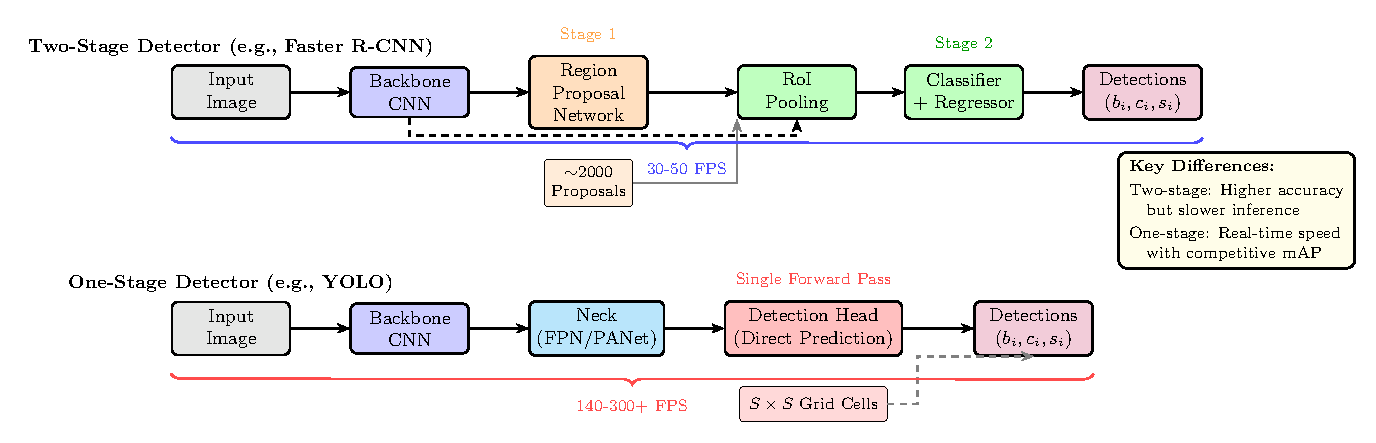
\includegraphics[width=0.95\textwidth]{figures/ch02_fig1_detector_comparison.pdf}
\caption{Architectural comparison between two-stage and one-stage object detectors. Two-stage detectors (top) process images through a Region Proposal Network to generate candidate regions before classification and refinement. One-stage detectors (bottom) directly predict bounding boxes and class probabilities in a single forward pass through the network, enabling significantly higher frame rates at the cost of some accuracy on challenging cases.}
\label{fig:detector_comparison}
\end{figure}

\subsection{Evolution of the YOLO Family}
\label{subsec:yolo_evolution}

The YOLO family of object detectors has undergone substantial evolution since its introduction, with each version incorporating architectural innovations, training improvements, and expanded capabilities. This progression reflects broader trends in deep learning research while maintaining the core philosophy of unified, real-time detection.

YOLOv1, introduced in 2016, established the foundational architecture by dividing images into an $S \times S$ grid, with each cell predicting $B$ bounding boxes and $C$ class probabilities. The network consisted of 24 convolutional layers followed by 2 fully connected layers, inspired by the GoogLeNet architecture. While revolutionary in its approach to real-time detection, YOLOv1 struggled with small objects and objects in close proximity due to the constraint that each grid cell could only predict a limited number of boxes.

YOLOv2, also known as YOLO9000, addressed several limitations of its predecessor through the introduction of batch normalization, anchor boxes derived from clustering on the training data, and multi-scale training. The Darknet-19 backbone replaced the original architecture, providing improved feature extraction while maintaining computational efficiency. The anchor box mechanism allowed the network to leverage prior knowledge about object aspect ratios, significantly improving localization accuracy.

YOLOv3 introduced multi-scale predictions by detecting objects at three different scales using feature pyramid concepts. The backbone evolved to Darknet-53, incorporating residual connections that enabled training of deeper networks. Binary cross-entropy loss replaced softmax for class predictions, enabling multi-label classification where objects could belong to multiple categories simultaneously. These changes substantially improved detection of small objects, which had been a persistent weakness.

YOLOv4 represented a comprehensive study of modern training techniques, incorporating numerous bag-of-freebies and bag-of-specials improvements. The architecture introduced CSPDarknet53 as the backbone, incorporating Cross Stage Partial connections that improved gradient flow while reducing computational cost. Path Aggregation Network (PANet) enhanced feature fusion across scales, while various data augmentation techniques including mosaic augmentation improved generalization. The Mish activation function and other refinements contributed to state-of-the-art accuracy while maintaining real-time performance.

YOLOv5, developed by Ultralytics, transitioned the implementation to PyTorch and introduced a family of models at different scales (nano, small, medium, large, extra-large) to accommodate varying computational budgets. The architecture employed a Focus layer for efficient downsampling and continued refinements to the backbone and neck architectures. Extensive hyperparameter optimization and training recipes contributed to strong out-of-the-box performance across diverse datasets.

YOLOv6 through YOLOv8 continued architectural innovations with efficient reparameterized backbones, decoupled detection heads, and anchor-free designs. YOLOv8 in particular unified detection, segmentation, and pose estimation within a single framework, demonstrating the versatility of the YOLO architecture for multiple vision tasks. The transition to anchor-free detection eliminated the need for hand-designed priors while maintaining detection quality.

YOLOv9 introduced Programmable Gradient Information (PGI) and Generalized Efficient Layer Aggregation Network (GELAN) to address information bottleneck problems in deep networks. These innovations improved gradient flow during training while maintaining inference efficiency, achieving state-of-the-art accuracy on the COCO benchmark.

YOLOv10 and YOLOv11 represent the current frontier, incorporating consistent dual assignments for NMS-free training and attention mechanisms for improved feature aggregation. These versions achieve unprecedented accuracy-latency trade-offs, with YOLOv11 demonstrating particular strength in small object detection and challenging visual conditions.

\begin{table}[htbp]
\centering
\caption{Evolution of YOLO Architectures: Key Characteristics and Performance Metrics}
\label{tab:yolo_comparison}
\begin{tabular}{lccccc}
\toprule
\textbf{Version} & \textbf{Year} & \textbf{Backbone} & \textbf{mAP$_{50}$} & \textbf{FPS} & \textbf{Key Innovation} \\
\midrule
YOLOv1 & 2016 & GoogLeNet-inspired & 63.4 & 45 & Unified detection \\
YOLOv2 & 2017 & Darknet-19 & 78.6 & 67 & Anchor boxes \\
YOLOv3 & 2018 & Darknet-53 & 57.9$^\dagger$ & 30 & Multi-scale prediction \\
YOLOv4 & 2020 & CSPDarknet53 & 65.7$^\dagger$ & 62 & BoF/BoS techniques \\
YOLOv5 & 2020 & CSPDarknet & 68.9$^\dagger$ & 140 & PyTorch ecosystem \\
YOLOv6 & 2022 & EfficientRep & 72.3$^\dagger$ & 175 & Reparameterization \\
YOLOv7 & 2022 & E-ELAN & 73.4$^\dagger$ & 161 & Extended ELAN \\
YOLOv8 & 2023 & CSPDarknet (mod) & 74.0$^\dagger$ & 280 & Anchor-free design \\
YOLOv9 & 2024 & GELAN & 75.5$^\dagger$ & 245 & PGI gradient flow \\
YOLOv10 & 2024 & CSPDarknet-ELAN & 76.1$^\dagger$ & 300 & NMS-free training \\
YOLOv11 & 2024 & C3k2-SPPF & 76.8$^\dagger$ & 320 & Attention mechanisms \\
\bottomrule
\multicolumn{6}{l}{\footnotesize $^\dagger$ mAP measured on COCO val2017 at 640$\times$640 resolution}
\end{tabular}
\end{table}

\subsection{Evaluation Metrics for Object Detection}
\label{subsec:eval_metrics}

Rigorous evaluation of object detection systems requires metrics that capture both localization accuracy and classification performance. The standard metrics employed in the field have evolved to address the unique challenges of evaluating detections across multiple scales and confidence thresholds.

\begin{definition}[Intersection over Union]
\label{def:iou}
The Intersection over Union (IoU), also known as the Jaccard index, measures the overlap between a predicted bounding box $b_p$ and a ground truth bounding box $b_g$:
\begin{equation}
\text{IoU}(b_p, b_g) = \frac{|b_p \cap b_g|}{|b_p \cup b_g|} = \frac{\text{Area of Intersection}}{\text{Area of Union}}
\end{equation}
where $|{\cdot}|$ denotes the area of a region. IoU ranges from 0 (no overlap) to 1 (perfect overlap).
\end{definition}

A detection is considered a true positive if its IoU with a ground truth box exceeds a predefined threshold (commonly 0.5 or 0.75) and the predicted class matches the ground truth class. Multiple detections of the same ground truth object are penalized, with only the highest-confidence detection counted as a true positive and subsequent detections treated as false positives.

\begin{definition}[Precision and Recall]
\label{def:precision_recall}
For a set of detections at a given confidence threshold, precision and recall are defined as:
\begin{equation}
\text{Precision} = \frac{TP}{TP + FP}, \quad \text{Recall} = \frac{TP}{TP + FN}
\end{equation}
where $TP$ denotes true positives (correct detections), $FP$ denotes false positives (incorrect detections or duplicates), and $FN$ denotes false negatives (missed objects).
\end{definition}

The precision-recall curve captures the trade-off between these metrics as the confidence threshold varies. As the threshold decreases, recall typically increases (more objects are detected) while precision may decrease (more false positives are included).

\begin{definition}[Average Precision]
\label{def:ap}
Average Precision (AP) summarizes the precision-recall curve as the area under the curve:
\begin{equation}
\text{AP} = \int_0^1 p(r) \, dr
\end{equation}
where $p(r)$ is the precision at recall level $r$. In practice, this is computed using an $n$-point interpolation:
\begin{equation}
\text{AP} = \frac{1}{n} \sum_{k=1}^{n} p_{\text{interp}}(r_k), \quad p_{\text{interp}}(r_k) = \max_{r \geq r_k} p(r)
\end{equation}
The COCO benchmark uses 101-point interpolation ($n=101$), while earlier benchmarks like PASCAL VOC used 11-point interpolation.
\end{definition}

\begin{definition}[Mean Average Precision]
\label{def:map}
Mean Average Precision (mAP) averages the AP across all $K$ object classes:
\begin{equation}
\text{mAP} = \frac{1}{K} \sum_{k=1}^{K} \text{AP}_k
\end{equation}
The COCO benchmark reports mAP averaged over multiple IoU thresholds from 0.5 to 0.95 in steps of 0.05, denoted mAP$_{50:95}$ or simply mAP. Additional metrics include mAP$_{50}$ (IoU threshold of 0.5) and mAP$_{75}$ (IoU threshold of 0.75), as well as scale-specific metrics mAP$_S$, mAP$_M$, and mAP$_L$ for small, medium, and large objects respectively.
\end{definition}

These metrics provide complementary views of detector performance. High mAP$_{50}$ indicates good object localization at a lenient threshold, while high mAP$_{75}$ requires precise bounding box predictions. The scale-specific metrics reveal performance characteristics across object sizes, which is particularly relevant for applications involving objects at varying distances or scales.

\section{Reinforcement Learning Preliminaries}
\label{sec:rl_preliminaries}

Reinforcement learning provides a principled framework for sequential decision-making under uncertainty, where an agent learns to maximize cumulative reward through interaction with an environment. This section develops the mathematical foundations necessary for applying RL to the optimization of synthetic data generation parameters.

\subsection{Markov Decision Processes}
\label{subsec:mdp}

The Markov Decision Process (MDP) provides the formal framework underlying most reinforcement learning algorithms. An MDP captures the essential elements of sequential decision-making: states, actions, transition dynamics, and rewards.

\begin{definition}[Markov Decision Process]
\label{def:mdp}
A Markov Decision Process is a tuple $\mathcal{M} = (\mathcal{S}, \mathcal{A}, P, R, \gamma)$ where:
\begin{itemize}
\item $\mathcal{S}$ is a set of states (the state space)
\item $\mathcal{A}$ is a set of actions (the action space)
\item $P: \mathcal{S} \times \mathcal{A} \times \mathcal{S} \rightarrow [0,1]$ is the transition probability function, where $P(s'|s,a)$ gives the probability of transitioning to state $s'$ when taking action $a$ in state $s$
\item $R: \mathcal{S} \times \mathcal{A} \rightarrow \mathbb{R}$ is the reward function, where $R(s,a)$ gives the expected immediate reward for taking action $a$ in state $s$
\item $\gamma \in [0,1)$ is the discount factor that determines the relative importance of immediate versus future rewards
\end{itemize}
The Markov property asserts that the future is conditionally independent of the past given the present: $P(s_{t+1}|s_t, a_t, s_{t-1}, a_{t-1}, \ldots) = P(s_{t+1}|s_t, a_t)$.
\end{definition}

The agent's behavior is governed by a policy, which specifies the action selection mechanism in each state.

\begin{definition}[Policy]
\label{def:policy}
A policy $\pi$ maps states to actions or action distributions. A deterministic policy $\pi: \mathcal{S} \rightarrow \mathcal{A}$ specifies a single action for each state. A stochastic policy $\pi: \mathcal{S} \times \mathcal{A} \rightarrow [0,1]$ specifies a probability distribution over actions, where $\pi(a|s)$ denotes the probability of selecting action $a$ in state $s$, satisfying $\sum_{a \in \mathcal{A}} \pi(a|s) = 1$ for all $s$.
\end{definition}

The objective in reinforcement learning is to find a policy that maximizes the expected cumulative discounted reward, known as the return.

\begin{definition}[Return and Value Functions]
\label{def:value_functions}
The return $G_t$ from time $t$ is the discounted sum of future rewards:
\begin{equation}
G_t = \sum_{k=0}^{\infty} \gamma^k R_{t+k+1} = R_{t+1} + \gamma R_{t+2} + \gamma^2 R_{t+3} + \cdots
\end{equation}
The state-value function $V^\pi(s)$ gives the expected return when starting in state $s$ and following policy $\pi$:
\begin{equation}
V^\pi(s) = \mathbb{E}_\pi[G_t | S_t = s] = \mathbb{E}_\pi\left[\sum_{k=0}^{\infty} \gamma^k R_{t+k+1} \Big| S_t = s\right]
\end{equation}
The action-value function $Q^\pi(s,a)$ gives the expected return when starting in state $s$, taking action $a$, and thereafter following policy $\pi$:
\begin{equation}
Q^\pi(s,a) = \mathbb{E}_\pi[G_t | S_t = s, A_t = a] = \mathbb{E}_\pi\left[\sum_{k=0}^{\infty} \gamma^k R_{t+k+1} \Big| S_t = s, A_t = a\right]
\end{equation}
\end{definition}

The value functions satisfy recursive relationships known as Bellman equations, which form the basis for many RL algorithms.

\begin{theorem}[Bellman Equations]
\label{thm:bellman}
For any policy $\pi$, the state-value function satisfies:
\begin{equation}
V^\pi(s) = \sum_{a \in \mathcal{A}} \pi(a|s) \left[ R(s,a) + \gamma \sum_{s' \in \mathcal{S}} P(s'|s,a) V^\pi(s') \right]
\end{equation}
The action-value function satisfies:
\begin{equation}
Q^\pi(s,a) = R(s,a) + \gamma \sum_{s' \in \mathcal{S}} P(s'|s,a) \sum_{a' \in \mathcal{A}} \pi(a'|s') Q^\pi(s',a')
\end{equation}
\end{theorem}

The optimal value functions, denoted $V^*(s)$ and $Q^*(s,a)$, represent the maximum achievable expected return from each state or state-action pair across all possible policies.

\begin{figure}[htbp]
\centering
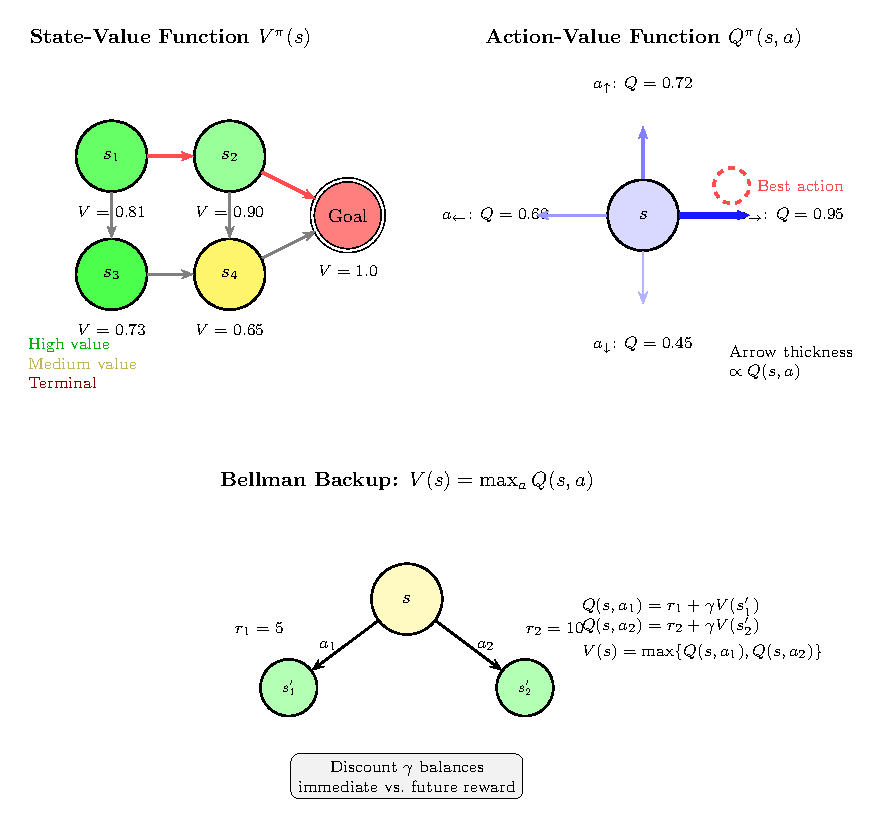
\includegraphics[width=0.9\textwidth]{figures/ch02_fig2_value_function.pdf}
\caption{Visualization of value functions in reinforcement learning. Left: The state-value function $V^\pi(s)$ assigns values to states based on expected future rewards under policy $\pi$. The optimal path (red arrows) follows states with highest values toward the goal. Center: The action-value function $Q^\pi(s,a)$ evaluates each possible action from a state; arrow thickness indicates action quality. Right: The Bellman backup illustrates how value estimates propagate through the state space via the recursive relationship between states and their successors.}
\label{fig:value_functions}
\end{figure}

% TikZ diagram for MDP state-action-reward cycle
\begin{figure}[htbp]
\centering
\begin{tikzpicture}[
    node distance=3cm,
    state/.style={circle, draw, minimum size=1.5cm, thick, fill=blue!10},
    action/.style={rectangle, draw, minimum size=1cm, thick, fill=green!10},
    arrow/.style={->, thick, >=stealth},
    label/.style={font=\small}
]

% Agent node
\node[state] (agent) {Agent};

% Environment node
\node[state, right=5cm of agent] (env) {Environment};

% Action arrow (top)
\draw[arrow, bend left=30] (agent.north east) to node[above, label] {Action $a_t$} (env.north west);

% State arrow (middle)
\draw[arrow, bend left=10] (env.west) to node[below, label, yshift=0.3cm] {State $s_{t+1}$} (agent.east);

% Reward arrow (bottom)
\draw[arrow, bend right=30] (env.south west) to node[below, label] {Reward $r_{t+1}$} (agent.south east);

% Policy annotation
\node[below=0.5cm of agent, align=center, font=\small] {Policy $\pi(a|s)$\\selects actions};

% Dynamics annotation
\node[below=0.5cm of env, align=center, font=\small] {Dynamics $P(s'|s,a)$\\determines transitions};

% Time step annotation
\node[above=1.5cm of agent, xshift=2.5cm, font=\footnotesize] {At each time step $t$:};
\node[above=0.9cm of agent, xshift=2.5cm, font=\footnotesize, align=left] {
1. Agent observes $s_t$\\
2. Agent selects $a_t \sim \pi(\cdot|s_t)$\\
3. Environment returns $r_{t+1}, s_{t+1}$
};

\end{tikzpicture}
\caption{The Markov Decision Process interaction loop. The agent observes the current state from the environment, selects an action according to its policy, and receives a reward along with the next state. This cycle repeats, with the agent's goal being to learn a policy that maximizes cumulative discounted reward.}
\label{fig:mdp_cycle}
\end{figure}

\subsection{Policy Gradient Methods}
\label{subsec:policy_gradient}

Policy gradient methods directly optimize a parameterized policy $\pi_\theta(a|s)$ by estimating gradients of the expected return with respect to the policy parameters $\theta$. These methods are particularly well-suited for continuous action spaces and can naturally handle stochastic policies.

The objective function to maximize is the expected return under the policy:
\begin{equation}
J(\theta) = \mathbb{E}_{\tau \sim \pi_\theta}[R(\tau)] = \mathbb{E}_{\tau \sim \pi_\theta}\left[\sum_{t=0}^{T} \gamma^t r_t\right]
\end{equation}
where $\tau = (s_0, a_0, r_1, s_1, a_1, \ldots)$ denotes a trajectory sampled by following policy $\pi_\theta$.

\begin{theorem}[Policy Gradient Theorem]
\label{thm:policy_gradient}
The gradient of the expected return with respect to policy parameters is:
\begin{equation}
\nabla_\theta J(\theta) = \mathbb{E}_{\tau \sim \pi_\theta}\left[\sum_{t=0}^{T} \nabla_\theta \log \pi_\theta(a_t|s_t) \cdot G_t\right]
\end{equation}
where $G_t = \sum_{k=t}^{T} \gamma^{k-t} r_k$ is the return from time $t$. This can be equivalently expressed as:
\begin{equation}
\nabla_\theta J(\theta) = \mathbb{E}_{s \sim d^\pi, a \sim \pi_\theta}\left[\nabla_\theta \log \pi_\theta(a|s) \cdot Q^{\pi_\theta}(s,a)\right]
\end{equation}
where $d^\pi$ is the stationary state distribution under policy $\pi$.
\end{theorem}

The basic policy gradient estimator, known as REINFORCE, suffers from high variance. Variance reduction techniques include using a baseline function $b(s)$ and the advantage function $A^\pi(s,a) = Q^\pi(s,a) - V^\pi(s)$.

\subsubsection{Trust Region Policy Optimization}

Trust Region Policy Optimization (TRPO) addresses the instability of vanilla policy gradient methods by constraining policy updates to a trust region that ensures monotonic improvement.

\begin{definition}[TRPO Optimization Problem]
\label{def:trpo}
TRPO solves the following constrained optimization problem at each iteration:
\begin{equation}
\begin{aligned}
\max_\theta \quad & \mathbb{E}_{s \sim d^{\pi_{\theta_\text{old}}}, a \sim \pi_{\theta_\text{old}}}\left[\frac{\pi_\theta(a|s)}{\pi_{\theta_\text{old}}(a|s)} A^{\pi_{\theta_\text{old}}}(s,a)\right] \\
\text{s.t.} \quad & \mathbb{E}_{s \sim d^{\pi_{\theta_\text{old}}}}\left[D_\text{KL}(\pi_{\theta_\text{old}}(\cdot|s) \| \pi_\theta(\cdot|s))\right] \leq \delta
\end{aligned}
\end{equation}
where $D_\text{KL}$ denotes the Kullback-Leibler divergence and $\delta$ is the trust region constraint.
\end{definition}

TRPO uses conjugate gradient descent and line search to approximately solve this constrained optimization problem, requiring computation of the Fisher information matrix.

\subsubsection{Proximal Policy Optimization}

Proximal Policy Optimization (PPO) simplifies TRPO by replacing the hard KL constraint with a clipped surrogate objective that achieves similar trust region effects without the computational complexity.

\begin{definition}[PPO Clipped Objective]
\label{def:ppo}
PPO maximizes the clipped surrogate objective:
\begin{equation}
L^\text{CLIP}(\theta) = \mathbb{E}_t\left[\min\left(r_t(\theta) \hat{A}_t, \text{clip}(r_t(\theta), 1-\epsilon, 1+\epsilon) \hat{A}_t\right)\right]
\end{equation}
where $r_t(\theta) = \frac{\pi_\theta(a_t|s_t)}{\pi_{\theta_\text{old}}(a_t|s_t)}$ is the probability ratio, $\hat{A}_t$ is an advantage estimate, and $\epsilon$ (typically 0.2) controls the clipping range.
\end{definition}

The clipping mechanism removes the incentive for moving the policy ratio outside the interval $[1-\epsilon, 1+\epsilon]$, effectively constraining the policy update. When the advantage is positive, the objective encourages increasing the probability of the action, but clips the benefit once $r_t(\theta) > 1+\epsilon$. When the advantage is negative, the objective encourages decreasing the probability, but clips once $r_t(\theta) < 1-\epsilon$.

\begin{algorithm}[htbp]
\caption{Proximal Policy Optimization (PPO)}
\label{alg:ppo}
\begin{algorithmic}[1]
\Require Initial policy parameters $\theta_0$, initial value function parameters $\phi_0$
\Require Clipping parameter $\epsilon$, number of epochs $K$, minibatch size $M$
\For{iteration $= 1, 2, \ldots$}
    \State Collect set of trajectories $\mathcal{D}_k$ by running policy $\pi_{\theta_k}$ in environment
    \State Compute rewards-to-go $\hat{R}_t$ for all timesteps in $\mathcal{D}_k$
    \State Compute advantage estimates $\hat{A}_t$ using GAE or other estimator
    \State Normalize advantages: $\hat{A}_t \leftarrow (\hat{A}_t - \mu_A) / \sigma_A$
    \For{epoch $= 1, \ldots, K$}
        \For{minibatch $\mathcal{B} \subset \mathcal{D}_k$ of size $M$}
            \State Compute policy ratio $r_t(\theta) = \pi_\theta(a_t|s_t) / \pi_{\theta_k}(a_t|s_t)$
            \State Compute clipped objective: $L^\text{CLIP} = \frac{1}{|\mathcal{B}|}\sum_t \min(r_t \hat{A}_t, \text{clip}(r_t, 1{\pm}\epsilon) \hat{A}_t)$
            \State Compute value loss: $L^\text{VF} = \frac{1}{|\mathcal{B}|}\sum_t (V_\phi(s_t) - \hat{R}_t)^2$
            \State Update $\theta$ by gradient ascent on $L^\text{CLIP}$
            \State Update $\phi$ by gradient descent on $L^\text{VF}$
        \EndFor
    \EndFor
\EndFor
\end{algorithmic}
\end{algorithm}

PPO has become the de facto standard for policy gradient methods due to its simplicity, stability, and competitive performance across a wide range of tasks. Its on-policy nature means that data collected under the current policy must be discarded after each update, which can limit sample efficiency in settings where environment interactions are expensive.

\subsection{Actor-Critic Architectures}
\label{subsec:actor_critic}

Actor-critic methods combine policy gradient approaches with value function estimation, using a learned value function (the critic) to reduce variance in policy gradient estimates while maintaining the flexibility of policy-based methods (the actor).

\begin{figure}[htbp]
\centering
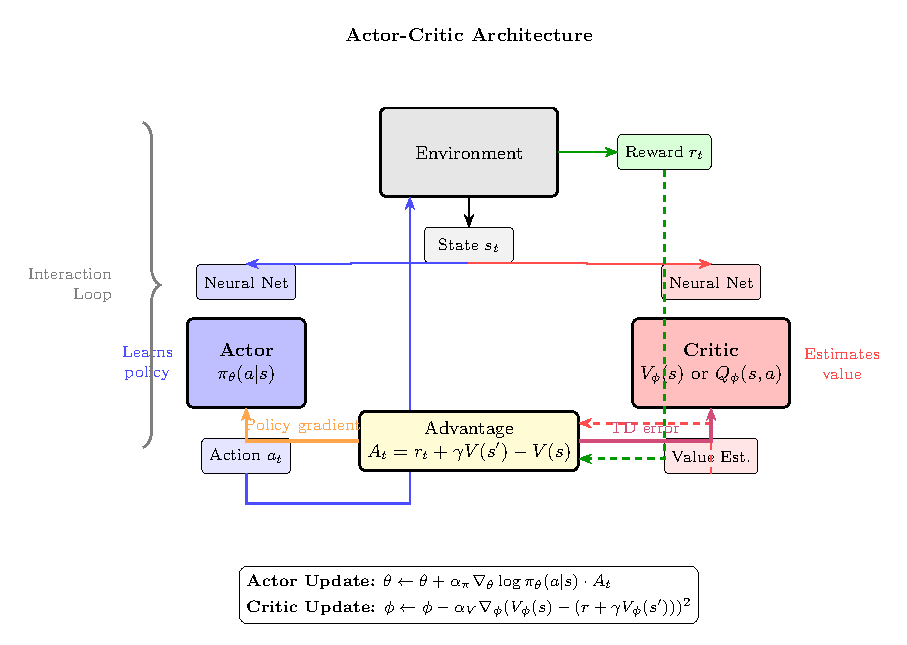
\includegraphics[width=0.85\textwidth]{figures/ch02_fig3_actor_critic.pdf}
\caption{The actor-critic architecture. The actor network learns a policy $\pi_\theta(a|s)$ that maps states to action distributions, while the critic network estimates the value function $V_\phi(s)$ or action-value function $Q_\phi(s,a)$. The temporal difference error computed from the critic's estimates provides a low-variance learning signal for updating the actor's policy parameters. This architecture combines the stability benefits of value-based methods with the flexibility of policy gradient approaches.}
\label{fig:actor_critic}
\end{figure}

\subsubsection{Soft Actor-Critic}

Soft Actor-Critic (SAC) is an off-policy actor-critic algorithm that incorporates entropy regularization to encourage exploration and improve robustness. The maximum entropy framework augments the standard RL objective with an entropy term.

\begin{definition}[Maximum Entropy Objective]
\label{def:max_entropy}
The maximum entropy reinforcement learning objective is:
\begin{equation}
J(\pi) = \sum_{t=0}^{T} \mathbb{E}_{(s_t, a_t) \sim \rho_\pi}\left[r(s_t, a_t) + \alpha \mathcal{H}(\pi(\cdot|s_t))\right]
\end{equation}
where $\mathcal{H}(\pi(\cdot|s)) = -\sum_a \pi(a|s) \log \pi(a|s)$ is the entropy of the policy and $\alpha > 0$ is the temperature parameter controlling the entropy-reward trade-off.
\end{definition}

SAC maintains three function approximators: a policy network $\pi_\theta$, and two Q-function networks $Q_{\phi_1}$, $Q_{\phi_2}$ (using the minimum to address overestimation bias). The soft value functions incorporate the entropy term.

\begin{definition}[Soft Bellman Equation]
\label{def:soft_bellman}
The soft Q-function satisfies the soft Bellman equation:
\begin{equation}
Q(s_t, a_t) = r(s_t, a_t) + \gamma \mathbb{E}_{s_{t+1}}\left[V(s_{t+1})\right]
\end{equation}
where the soft value function is:
\begin{equation}
V(s_t) = \mathbb{E}_{a_t \sim \pi}\left[Q(s_t, a_t) - \alpha \log \pi(a_t|s_t)\right]
\end{equation}
\end{definition}

SAC's off-policy nature allows it to reuse past experience stored in a replay buffer, providing substantial sample efficiency improvements over on-policy methods. The entropy regularization prevents premature convergence and maintains exploration throughout training.

\begin{algorithm}[htbp]
\caption{Soft Actor-Critic (SAC)}
\label{alg:sac}
\begin{algorithmic}[1]
\Require Initial policy parameters $\theta$, Q-function parameters $\phi_1, \phi_2$
\Require Target Q-function parameters $\bar{\phi}_1 \leftarrow \phi_1$, $\bar{\phi}_2 \leftarrow \phi_2$
\Require Empty replay buffer $\mathcal{D}$, learning rates $\lambda_Q$, $\lambda_\pi$, $\lambda_\alpha$
\For{each iteration}
    \For{each environment step}
        \State Sample action $a_t \sim \pi_\theta(\cdot|s_t)$
        \State Execute $a_t$, observe $r_t$, $s_{t+1}$
        \State Store $(s_t, a_t, r_t, s_{t+1})$ in $\mathcal{D}$
    \EndFor
    \For{each gradient step}
        \State Sample minibatch $\mathcal{B} = \{(s, a, r, s')\}$ from $\mathcal{D}$
        \State Compute target: $y = r + \gamma(\min_{i=1,2} Q_{\bar{\phi}_i}(s', \tilde{a}') - \alpha \log \pi_\theta(\tilde{a}'|s'))$ where $\tilde{a}' \sim \pi_\theta(\cdot|s')$
        \State Update Q-functions: $\phi_i \leftarrow \phi_i - \lambda_Q \nabla_{\phi_i} \frac{1}{|\mathcal{B}|}\sum(Q_{\phi_i}(s,a) - y)^2$
        \State Update policy: $\theta \leftarrow \theta + \lambda_\pi \nabla_\theta \frac{1}{|\mathcal{B}|}\sum(\alpha \log \pi_\theta(\tilde{a}|s) - \min_{i} Q_{\phi_i}(s, \tilde{a}))$
        \State Update temperature: $\alpha \leftarrow \alpha - \lambda_\alpha \nabla_\alpha \frac{1}{|\mathcal{B}|}\sum(-\alpha \log \pi_\theta(\tilde{a}|s) - \alpha \bar{\mathcal{H}})$
        \State Update targets: $\bar{\phi}_i \leftarrow \tau \phi_i + (1-\tau)\bar{\phi}_i$
    \EndFor
\EndFor
\end{algorithmic}
\end{algorithm}

\subsubsection{Twin Delayed Deep Deterministic Policy Gradient}

Twin Delayed Deep Deterministic Policy Gradient (TD3) addresses overestimation bias and instability in deterministic policy gradient methods through three key modifications: clipped double Q-learning, delayed policy updates, and target policy smoothing.

\begin{definition}[TD3 Modifications]
\label{def:td3}
TD3 incorporates three modifications to DDPG:
\begin{enumerate}
\item \textbf{Clipped Double Q-learning}: Use the minimum of two Q-networks for computing the target:
\begin{equation}
y = r + \gamma \min_{i=1,2} Q_{\bar{\phi}_i}(s', \pi_{\bar{\theta}}(s'))
\end{equation}
\item \textbf{Delayed Policy Updates}: Update the policy network less frequently than the Q-networks (typically every 2 Q-updates).
\item \textbf{Target Policy Smoothing}: Add noise to target actions to prevent exploitation of Q-function errors:
\begin{equation}
\tilde{a}' = \pi_{\bar{\theta}}(s') + \text{clip}(\epsilon, -c, c), \quad \epsilon \sim \mathcal{N}(0, \sigma^2)
\end{equation}
\end{enumerate}
\end{definition}

TD3 is particularly effective for continuous control tasks where deterministic policies are appropriate. The combination of techniques provides more stable learning than DDPG while maintaining its sample efficiency advantages.

\subsection{Off-Policy Versus On-Policy Learning}
\label{subsec:off_on_policy}

The distinction between off-policy and on-policy learning has significant implications for sample efficiency, stability, and applicability to different problem settings.

On-policy methods, including REINFORCE, A2C, TRPO, and PPO, learn from data collected under the current policy. After each policy update, previously collected data becomes stale and must be discarded because the importance weights required for off-policy correction become highly variable. This constraint limits sample efficiency but provides stable learning dynamics and unbiased gradient estimates.

Off-policy methods, including DQN, DDPG, SAC, and TD3, can learn from data collected under any policy, enabling the use of experience replay buffers that store past transitions. This dramatically improves sample efficiency by allowing each transition to contribute to multiple gradient updates. However, off-policy learning introduces challenges including the deadly triad (function approximation, bootstrapping, and off-policy learning) that can lead to instability.

\begin{table}[htbp]
\centering
\caption{Comparison of On-Policy and Off-Policy Reinforcement Learning}
\label{tab:on_off_policy}
\begin{tabular}{lcc}
\toprule
\textbf{Characteristic} & \textbf{On-Policy} & \textbf{Off-Policy} \\
\midrule
Sample efficiency & Lower & Higher \\
Learning stability & More stable & Can be unstable \\
Experience replay & Not directly usable & Fully utilized \\
Exploration & Via policy stochasticity & Via replay diversity \\
Gradient bias & Unbiased & Requires correction \\
Representative algorithms & PPO, TRPO, A2C & SAC, TD3, DQN \\
\bottomrule
\end{tabular}
\end{table}

For the problem of optimizing synthetic data generation parameters, sample efficiency is paramount because each evaluation requires training a detection model, a computationally expensive operation. This consideration favors off-policy methods such as SAC, though the relatively low-dimensional action space (generator parameters) may also make sample-efficient variants of on-policy methods viable.

\section{Bayesian Optimization}
\label{sec:bayesian_optimization}

Bayesian optimization provides an alternative paradigm for black-box optimization that is particularly well-suited for expensive objective functions. Unlike reinforcement learning, which learns a policy for sequential decision-making, Bayesian optimization directly models the objective function and uses this model to guide the search for optimal parameters.

\subsection{Gaussian Processes as Surrogate Models}
\label{subsec:gaussian_processes}

The core idea of Bayesian optimization is to construct a probabilistic surrogate model of the objective function based on observed evaluations, then use this model to decide where to evaluate next. Gaussian Processes (GPs) are the most common choice for surrogate models due to their flexibility and principled uncertainty quantification.

\begin{definition}[Gaussian Process]
\label{def:gp}
A Gaussian Process is a collection of random variables, any finite number of which have a joint Gaussian distribution. A GP is fully specified by its mean function $m(x)$ and covariance function (kernel) $k(x, x')$:
\begin{equation}
f(x) \sim \mathcal{GP}(m(x), k(x, x'))
\end{equation}
where $m(x) = \mathbb{E}[f(x)]$ and $k(x, x') = \mathbb{E}[(f(x) - m(x))(f(x') - m(x'))]$.
\end{definition}

Given observations $\mathcal{D} = \{(x_i, y_i)\}_{i=1}^{n}$ where $y_i = f(x_i) + \epsilon$ with $\epsilon \sim \mathcal{N}(0, \sigma^2_n)$, the posterior distribution over function values at a new point $x_*$ is Gaussian:
\begin{equation}
f(x_*) | \mathcal{D} \sim \mathcal{N}(\mu(x_*), \sigma^2(x_*))
\end{equation}
with posterior mean and variance:
\begin{align}
\mu(x_*) &= m(x_*) + k(x_*, X)(K + \sigma^2_n I)^{-1}(y - m(X)) \\
\sigma^2(x_*) &= k(x_*, x_*) - k(x_*, X)(K + \sigma^2_n I)^{-1}k(X, x_*)
\end{align}
where $K$ is the kernel matrix with $K_{ij} = k(x_i, x_j)$.

The choice of kernel encodes prior assumptions about the function's properties. The squared exponential (RBF) kernel $k(x, x') = \sigma^2_f \exp\left(-\frac{\|x-x'\|^2}{2\ell^2}\right)$ assumes smooth functions, while the Mat\'{e}rn kernel allows control over differentiability.

\subsection{Acquisition Functions}
\label{subsec:acquisition_functions}

Acquisition functions use the posterior distribution to quantify the utility of evaluating the objective at different points, balancing exploration of uncertain regions with exploitation of promising areas.

\begin{definition}[Expected Improvement]
\label{def:ei}
Expected Improvement (EI) measures the expected amount by which a new evaluation will improve upon the current best observation $f^* = \max_{i} y_i$:
\begin{equation}
\text{EI}(x) = \mathbb{E}[\max(f(x) - f^*, 0)] = (μ(x) - f^*)\Phi(Z) + \sigma(x)\phi(Z)
\end{equation}
where $Z = \frac{\mu(x) - f^*}{\sigma(x)}$, and $\Phi$, $\phi$ are the CDF and PDF of the standard normal distribution.
\end{definition}

\begin{definition}[Upper Confidence Bound]
\label{def:ucb}
Upper Confidence Bound (UCB) selects points that maximize an optimistic estimate of the function value:
\begin{equation}
\text{UCB}(x) = \mu(x) + \beta \sigma(x)
\end{equation}
where $\beta > 0$ controls the exploration-exploitation trade-off. Larger $\beta$ favors exploration of uncertain regions.
\end{definition}

Other acquisition functions include Probability of Improvement (PI), Thompson Sampling, and Knowledge Gradient. The optimal acquisition function depends on problem characteristics including noise level, evaluation budget, and the relative costs of exploration versus exploitation.

% TikZ diagram for Gaussian Process with acquisition function
\begin{figure}[htbp]
\centering
\begin{tikzpicture}[scale=0.9]
    % Draw axes
    \draw[->] (-0.5, 0) -- (10, 0) node[right] {$x$};
    \draw[->] (0, -1) -- (0, 5) node[above] {$f(x)$};

    % True function (hidden, dashed)
    \draw[dashed, gray, thick] plot[smooth, tension=0.7] coordinates {
        (0.5, 2) (2, 3.5) (3.5, 2.5) (5, 4) (6.5, 3) (8, 3.8) (9.5, 2.5)
    };

    % GP mean function
    \draw[blue, very thick] plot[smooth, tension=0.7] coordinates {
        (0.5, 2.1) (2, 3.4) (3.5, 2.6) (5, 3.2) (6.5, 2.8) (8, 3.5) (9.5, 2.8)
    };

    % GP uncertainty (shaded region)
    \fill[blue!20, opacity=0.5] plot[smooth, tension=0.7] coordinates {
        (0.5, 2.4) (2, 3.7) (3.5, 3.0) (5, 4.0) (6.5, 3.6) (8, 3.8) (9.5, 3.5)
    } -- plot[smooth, tension=0.7] coordinates {
        (9.5, 2.1) (8, 3.2) (6.5, 2.0) (5, 2.4) (3.5, 2.2) (2, 3.1) (0.5, 1.8)
    } -- cycle;

    % Observed points
    \fill[red] (2, 3.5) circle (3pt);
    \fill[red] (3.5, 2.5) circle (3pt);
    \fill[red] (8, 3.8) circle (3pt);

    % Next evaluation point (from acquisition function)
    \draw[green!60!black, very thick, ->] (5, -0.5) -- (5, 0.3);
    \node[green!60!black, below] at (5, -0.5) {Next $x$};

    % Acquisition function (bottom subplot)
    \begin{scope}[yshift=-3cm]
        \draw[->] (-0.5, 0) -- (10, 0) node[right] {$x$};
        \draw[->] (0, -0.2) -- (0, 2) node[above] {$\alpha(x)$};

        % EI acquisition function
        \draw[orange, very thick] plot[smooth, tension=0.7] coordinates {
            (0.5, 0.2) (2, 0.1) (3.5, 0.3) (5, 1.5) (6.5, 0.8) (8, 0.1) (9.5, 0.4)
        };

        % Maximum of acquisition function
        \fill[green!60!black] (5, 1.5) circle (3pt);
    \end{scope}

    % Labels
    \node[blue, right] at (9.5, 3.8) {$\mu(x) \pm \sigma(x)$};
    \node[gray, right] at (9.5, 2.2) {True $f(x)$};
    \node[red, right] at (8.3, 3.8) {Observations};
    \node[orange, right] at (9.5, -1.5) {EI$(x)$};

\end{tikzpicture}
\caption{Bayesian optimization with a Gaussian Process surrogate model. The top panel shows the GP posterior mean (blue line) with uncertainty bounds (shaded region) based on three observations (red points). The dashed gray line represents the unknown true function. The bottom panel shows the Expected Improvement acquisition function, which peaks at regions of high uncertainty and predicted improvement. The next evaluation point is selected at the acquisition function maximum.}
\label{fig:gp_acquisition}
\end{figure}

\subsection{The Exploration-Exploitation Trade-off}
\label{subsec:exploration_exploitation}

The exploration-exploitation trade-off is fundamental to both Bayesian optimization and reinforcement learning, though it manifests differently in each setting.

In Bayesian optimization, exploration refers to evaluating points where the surrogate model has high uncertainty, potentially discovering better regions of the search space. Exploitation refers to evaluating points where the model predicts high objective values, refining the estimate of the optimum. Acquisition functions implicitly balance these objectives: EI naturally incorporates both through its dependence on both the mean (exploitation) and variance (exploration), while UCB provides explicit control through the $\beta$ parameter.

\begin{theorem}[Regret Bounds for GP-UCB]
\label{thm:gp_ucb_regret}
For a function $f$ sampled from a GP with bounded RKHS norm, the GP-UCB algorithm with appropriately chosen $\beta_t$ achieves sublinear cumulative regret:
\begin{equation}
R_T = \sum_{t=1}^{T} (f(x^*) - f(x_t)) = \mathcal{O}^*(\sqrt{T \gamma_T})
\end{equation}
where $\gamma_T$ is the maximum information gain and $\mathcal{O}^*$ hides logarithmic factors. For the squared exponential kernel in $d$ dimensions, $\gamma_T = \mathcal{O}((\log T)^{d+1})$.
\end{theorem}

This theoretical guarantee ensures that Bayesian optimization converges to the optimum, with the rate depending on the complexity of the function class through the information gain term.

\subsection{Comparison with Reinforcement Learning Approaches}
\label{subsec:bo_vs_rl}

Bayesian optimization and reinforcement learning offer complementary approaches to the problem of optimizing synthetic data generator parameters. Understanding their relative strengths guides the selection of appropriate methods.

Bayesian optimization excels when the objective function is expensive to evaluate, the parameter space is relatively low-dimensional (typically fewer than 20 dimensions), and the optimization is stateless (each evaluation is independent). The method provides principled uncertainty quantification and achieves strong theoretical guarantees on sample efficiency.

Reinforcement learning is preferred when the optimization involves sequential decision-making with state dependence, the action space is high-dimensional, or the problem structure allows for policy generalization across similar tasks. RL can also leverage partial feedback and intermediate rewards, which may not be available in pure black-box optimization.

For synthetic data optimization, both approaches have merit. The problem can be framed as stateless black-box optimization (favoring BO) if we optimize generator parameters for a single training run, or as sequential decision-making (favoring RL) if we adaptively adjust parameters during the course of dataset generation based on observed detection performance.

\begin{table}[htbp]
\centering
\caption{Comparison of Bayesian Optimization and Reinforcement Learning for Parameter Optimization}
\label{tab:bo_vs_rl}
\begin{tabular}{lcc}
\toprule
\textbf{Characteristic} & \textbf{Bayesian Optimization} & \textbf{Reinforcement Learning} \\
\midrule
Problem structure & Stateless, black-box & Sequential, state-dependent \\
Dimensionality & Low ($\lesssim 20$) & Higher tolerated \\
Sample efficiency & Very high & Moderate to high \\
Uncertainty quantification & Principled (GP posterior) & Implicit (policy entropy) \\
Intermediate feedback & Not utilized & Can be leveraged \\
Theoretical guarantees & Strong (regret bounds) & Weaker (convergence) \\
Parallelization & Batch acquisition & Distributed rollouts \\
\bottomrule
\end{tabular}
\end{table}

Hybrid approaches combining elements of both paradigms have shown promise. BOHB (Bayesian Optimization HyperBand) combines Bayesian optimization with multi-fidelity evaluation, while methods like Neural Architecture Search use RL to search over discrete structures with BO for continuous hyperparameters.

\section{Domain Randomization Theory}
\label{sec:domain_randomization}

Domain randomization has emerged as a powerful technique for training models on synthetic data that transfer effectively to real-world settings. This section develops the theoretical foundations of domain randomization, drawing on recent work that provides formal guarantees for sim-to-real transfer.

\subsection{Formal Framework for Domain Randomization}
\label{subsec:dr_framework}

The theoretical framework for understanding domain randomization models the simulator as a family of environments parameterized by unknown physical and visual parameters. The key insight is that by training on a sufficiently diverse distribution over these parameters, the policy learns to be robust to the specific parameter values encountered in the real world.

\begin{definition}[Domain Randomization Framework]
\label{def:dr_framework}
Consider a family of MDPs $\{\mathcal{M}_\xi\}_{\xi \in \Xi}$ indexed by domain parameters $\xi$ (representing physical properties, visual appearance, etc.). Let $P_\Xi$ be a distribution over domain parameters. Domain randomization trains a policy $\pi$ on the mixture MDP:
\begin{equation}
\mathcal{M}_{DR} = \int_\Xi \mathcal{M}_\xi \, dP_\Xi(\xi)
\end{equation}
The goal is that a policy performing well under $\mathcal{M}_{DR}$ will also perform well on the real-world MDP $\mathcal{M}_{\xi^*}$ for unknown $\xi^* \in \Xi$.
\end{definition}

The ICLR 2022 paper ``Understanding Domain Randomization for Sim-to-real Transfer'' established formal conditions under which domain randomization succeeds. The key result demonstrates that under mild assumptions, domain randomization can achieve zero-shot transfer without any real-world training data.

\begin{theorem}[Domain Randomization Transfer]
\label{thm:dr_transfer}
Let $\pi^*_{DR}$ be an optimal policy for the domain-randomized MDP $\mathcal{M}_{DR}$, and let $\mathcal{M}_{\xi^*}$ be the real-world MDP with $\xi^* \in \Xi$. Under the assumption that the optimal Q-function varies smoothly with domain parameters, the performance gap satisfies:
\begin{equation}
V^*_{\xi^*} - V^{\pi^*_{DR}}_{\xi^*} \leq C \cdot d(\xi^*, \text{supp}(P_\Xi))
\end{equation}
where $V^*_{\xi^*}$ is the optimal value in the real world, $V^{\pi^*_{DR}}_{\xi^*}$ is the value of the domain-randomized policy in the real world, $C$ is a Lipschitz constant, and $d(\cdot, \cdot)$ measures distance to the support of the randomization distribution.
\end{theorem}

This theorem provides a formal justification for domain randomization: if the randomization distribution $P_\Xi$ has support containing or near the real-world parameters $\xi^*$, the transfer gap is bounded.

\subsection{Why Randomization Enables Generalization}
\label{subsec:why_randomization}

The effectiveness of domain randomization can be understood through several complementary perspectives that illuminate why introducing variability in synthetic data improves generalization to real-world conditions.

From a robustness perspective, training on diverse domain parameters forces the policy to rely on features that are consistent across variations rather than domain-specific artifacts. For object detection, this means learning to recognize objects based on their shape and geometric structure rather than spurious correlations with specific textures, lighting conditions, or background patterns.

From a coverage perspective, sufficient randomization ensures that the real-world domain appears as ``just another variation'' within the training distribution. If the randomization spans a sufficiently wide range of visual and physical parameters, the gap between simulation and reality becomes a small perturbation that well-trained models can tolerate.

From a regularization perspective, domain randomization acts as a form of implicit regularization that prevents overfitting to specific characteristics of the simulated environment. This is analogous to data augmentation techniques in supervised learning, but applied at the level of the entire rendering and physics pipeline rather than individual images.

The theoretical framework also highlights the importance of using memory or recurrent policies when dealing with partially observable domains. Memoryless policies cannot distinguish between different domain parameters from single observations, which can lead to suboptimal behavior. History-dependent policies can implicitly infer domain characteristics from sequences of observations and adapt their behavior accordingly.

\subsection{Structured Versus Unstructured Randomization}
\label{subsec:structured_unstructured}

A critical distinction in domain randomization is between unstructured (uniform) randomization and structured randomization that respects the underlying constraints and correlations of the domain.

Unstructured randomization independently samples each parameter from a predefined range, typically uniform or Gaussian distributions. This approach is simple to implement and provides broad coverage of the parameter space, but can generate physically implausible or semantically inconsistent configurations. For example, independently randomizing object positions may place objects inside each other or floating in mid-air.

\begin{definition}[Unstructured Domain Randomization]
\label{def:unstructured_dr}
Unstructured domain randomization samples domain parameters independently:
\begin{equation}
\xi = (\xi_1, \ldots, \xi_d), \quad \xi_i \sim P_i \text{ independently}
\end{equation}
where each $P_i$ is typically a uniform or Gaussian distribution over the valid range of parameter $i$.
\end{definition}

Structured Domain Randomization (SDR), introduced by NVIDIA researchers, incorporates domain knowledge to generate more realistic variations. SDR samples from conditional distributions that respect scene semantics: objects are placed on surfaces, lighting follows physical constraints, and spatial relationships are preserved. This produces training data that, while still diverse, remains within the manifold of plausible scenes.

\begin{definition}[Structured Domain Randomization]
\label{def:structured_dr}
Structured domain randomization samples domain parameters from a joint distribution that encodes domain constraints:
\begin{equation}
\xi \sim P_\Xi(\xi_1, \ldots, \xi_d | \mathcal{C})
\end{equation}
where $\mathcal{C}$ represents structural constraints such as physical plausibility, semantic consistency, and spatial relationships.
\end{definition}

Empirical results demonstrate that SDR achieves better transfer performance than unstructured randomization, particularly when training data is limited. On the KITTI benchmark for vehicle detection, SDR trained entirely on synthetic data outperformed both unstructured domain randomization and alternative synthetic data sources.

The trade-off between structured and unstructured approaches involves coverage versus plausibility. Unstructured randomization may expose the model to edge cases that improve robustness, while structured randomization focuses capacity on the plausible region of the domain space. The optimal choice depends on the specific application and the degree of mismatch between simulation and reality.

% TikZ diagram for domain randomization conceptual diagram
\begin{figure}[htbp]
\centering
\begin{tikzpicture}[scale=0.85]
    % Simulation domain (large ellipse on left)
    \draw[thick, blue, fill=blue!10] (-4, 0) ellipse (3cm and 2.5cm);
    \node[blue, font=\bfseries] at (-4, 3) {Simulation Domain};

    % Real world domain (smaller ellipse on right)
    \draw[thick, red, fill=red!10] (4, 0) ellipse (2cm and 1.5cm);
    \node[red, font=\bfseries] at (4, 2) {Real World};

    % Randomization distribution (contained in simulation)
    \draw[thick, green!60!black, dashed] (-4, 0) ellipse (2.5cm and 2cm);
    \node[green!60!black, font=\small] at (-4, -2.5) {Randomization $P_\Xi$};

    % Sample points in randomization distribution
    \foreach \i in {1,...,15} {
        \pgfmathsetmacro{\rx}{-4 + 2*rand}
        \pgfmathsetmacro{\ry}{1.5*rand}
        \fill[green!60!black] (\rx, \ry) circle (2pt);
    }

    % Real world point
    \fill[red] (4, 0) circle (4pt);
    \node[red, font=\small, below] at (4, -0.3) {$\xi^*$};

    % Arrow showing transfer
    \draw[thick, ->, >=stealth] (-0.5, 0) -- (1.5, 0);
    \node[above, font=\small] at (0.5, 0.2) {Transfer};

    % Policy learned on randomized data
    \node[font=\small, align=center] at (-4, 0) {Policy $\pi$\\learns invariant\\features};

    % Annotations
    \draw[thick, <->, >=stealth] (-1.5, -2) -- (2, -2);
    \node[below, font=\small] at (0.25, -2) {Domain Gap};

    % Coverage annotation
    \draw[thick, <-] (-6.5, 1) -- (-5.5, 0.5);
    \node[left, font=\small, align=right] at (-6.5, 1) {Wide coverage\\ensures real\\is ``just another\\variation''};

\end{tikzpicture}
\caption{Conceptual illustration of domain randomization. The policy is trained on synthetic data sampled from a distribution $P_\Xi$ over domain parameters (green region). If the distribution provides sufficient coverage and the real-world parameters $\xi^*$ fall within or near this distribution, the policy transfers successfully. The domain gap between simulation and reality is bridged by training on diverse variations.}
\label{fig:domain_randomization}
\end{figure}

\subsection{The Role of Memory in Sim-to-Real Transfer}
\label{subsec:memory_sim2real}

The theoretical analysis of domain randomization reveals a fundamental role for memory in achieving successful sim-to-real transfer. When domain parameters are not directly observable, history-dependent policies can substantially outperform memoryless policies by implicitly inferring domain characteristics from past observations.

Consider a setting where the friction coefficient is unknown but affects the dynamics of object manipulation. A memoryless policy must use a single action for all friction values, leading to suboptimal behavior. A recurrent policy can observe the effects of its actions and infer the friction coefficient, then adapt its strategy accordingly.

\begin{theorem}[Advantage of Memory in Domain Randomization]
\label{thm:memory_advantage}
For domain-randomized MDPs with unobservable domain parameters, let $V^*_{mem}$ denote the optimal value achievable by history-dependent policies and $V^*_{memless}$ denote the optimal value for memoryless policies. Then:
\begin{equation}
V^*_{mem} - V^*_{memless} \geq 0
\end{equation}
with strict inequality when the optimal action depends on unobservable domain parameters.
\end{theorem}

This result has practical implications for architecture design. When using domain randomization for sim-to-real transfer, recurrent neural networks (LSTMs, GRUs) or attention-based architectures that can process sequences of observations may achieve better transfer than feedforward networks. The policy can learn to extract domain-relevant information from the observation history and condition its behavior on this implicit domain estimate.

For object detection specifically, while individual frame processing is typical, incorporating temporal context through video-based detection or tracking-by-detection approaches may improve robustness to domain shift by allowing the model to adapt to the statistics of the target domain during inference.

\section{Multi-Fidelity Optimization}
\label{sec:multi_fidelity}

Multi-fidelity optimization methods exploit the availability of cheaper, lower-fidelity approximations to the expensive target objective. In the context of synthetic data optimization, lower fidelity might correspond to training with fewer images, fewer epochs, smaller model sizes, or reduced image resolution. These methods can dramatically reduce the total computational cost of optimization.

\subsection{Successive Halving Algorithm}
\label{subsec:successive_halving}

Successive Halving provides a principled approach to allocating resources among a set of configurations by iteratively eliminating the worst performers.

\begin{definition}[Successive Halving]
\label{def:successive_halving}
Given $n$ configurations and a total budget $B$, Successive Halving proceeds as follows:
\begin{enumerate}
\item Initialize: $S_0 = \{$all $n$ configurations$\}$, budget per configuration $r_0 = B/(n \lceil \log_\eta n \rceil)$
\item For round $k = 0, 1, \ldots, \lceil \log_\eta n \rceil - 1$:
    \begin{enumerate}
    \item Evaluate each configuration in $S_k$ with budget $r_k$
    \item Keep top $1/\eta$ fraction: $S_{k+1} = \text{top}_{|S_k|/\eta}(S_k)$
    \item Increase budget: $r_{k+1} = r_k \cdot \eta$
    \end{enumerate}
\item Return the best configuration from $S_{\lceil \log_\eta n \rceil}$
\end{enumerate}
where $\eta > 1$ is the reduction factor (typically $\eta = 3$).
\end{definition}

\begin{algorithm}[htbp]
\caption{Successive Halving}
\label{alg:successive_halving}
\begin{algorithmic}[1]
\Require Set of configurations $\mathcal{C}$, total budget $B$, reduction factor $\eta$
\State $n \leftarrow |\mathcal{C}|$, $s_{\max} \leftarrow \lfloor \log_\eta n \rfloor$
\State $r \leftarrow B / (n \cdot (s_{\max} + 1))$ \Comment{Initial budget per configuration}
\State $S \leftarrow \mathcal{C}$ \Comment{Active configurations}
\For{$k = 0, 1, \ldots, s_{\max}$}
    \State $n_k \leftarrow \lfloor n / \eta^k \rfloor$ \Comment{Number of configurations in round $k$}
    \State $r_k \leftarrow r \cdot \eta^k$ \Comment{Budget per configuration in round $k$}
    \State $L \leftarrow \{(\text{config}, \text{Evaluate}(\text{config}, r_k)) : \text{config} \in S\}$
    \State $S \leftarrow \text{top}_{n_k / \eta}(L)$ \Comment{Keep best $n_k/\eta$ configurations}
\EndFor
\State \Return Configuration in $S$ with best final evaluation
\end{algorithmic}
\end{algorithm}

The key assumption underlying Successive Halving is that the ranking of configurations is approximately preserved across fidelity levels: configurations that perform well with small budgets tend to perform well with larger budgets. When this assumption holds, Successive Halving can identify the best configuration with far less total computation than exhaustive evaluation.

\begin{figure}[htbp]
\centering
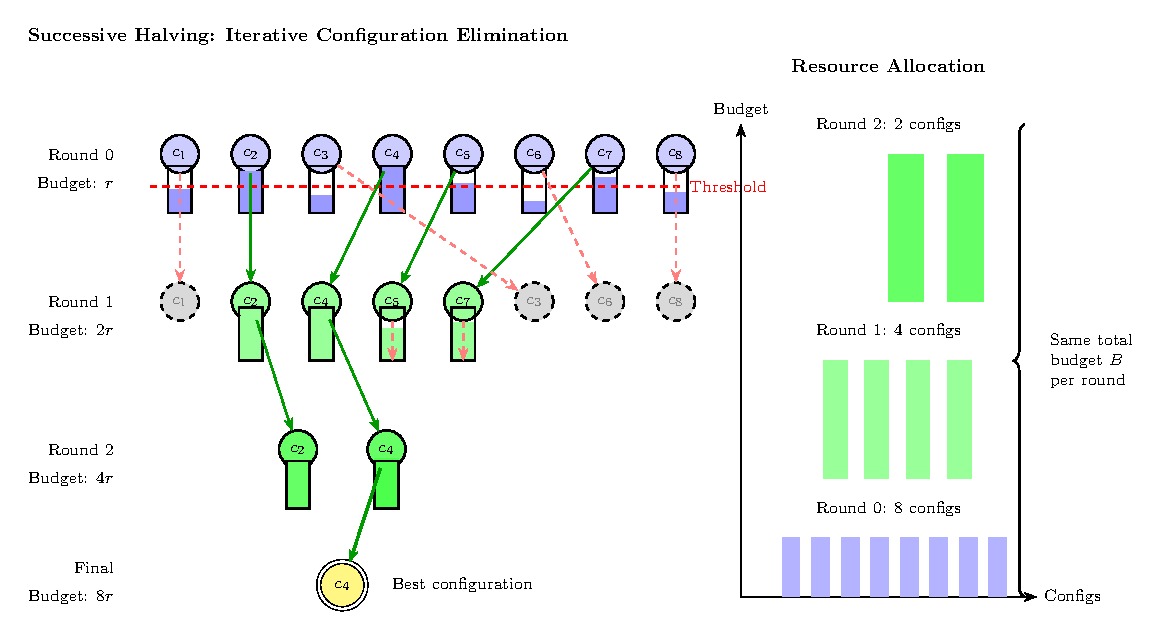
\includegraphics[width=0.95\textwidth]{figures/ch02_fig4_successive_halving.pdf}
\caption{Successive Halving for multi-fidelity hyperparameter optimization. Left: The algorithm iteratively evaluates configurations with increasing budgets while eliminating the bottom half at each round. Starting with 8 configurations (Round 0), only 4 survive to Round 1, then 2 to Round 2, with the final round identifying the best configuration. Right: Resource allocation across rounds shows how the same total budget is distributed---initially spread across many configurations with small budgets, then concentrated on fewer promising configurations with larger budgets. This approach efficiently explores the configuration space while avoiding wasted computation on poor performers.}
\label{fig:successive_halving}
\end{figure}

\subsection{Hyperband Framework}
\label{subsec:hyperband}

Hyperband addresses a fundamental limitation of Successive Halving: the algorithm requires specifying the number of configurations $n$ in advance, which implicitly determines the trade-off between exploration (many configurations, small initial budgets) and exploitation (few configurations, large initial budgets).

\begin{definition}[Hyperband]
\label{def:hyperband}
Hyperband runs multiple instances of Successive Halving with different exploration-exploitation trade-offs:
\begin{equation}
s \in \{s_{\max}, s_{\max}-1, \ldots, 0\}
\end{equation}
where $s_{\max} = \lfloor \log_\eta(R) \rfloor$ and $R$ is the maximum budget per configuration. For each $s$, Successive Halving is run with:
\begin{align}
n_s &= \left\lceil \frac{(s_{\max} + 1) \cdot \eta^s}{s + 1} \right\rceil \text{ configurations} \\
r_s &= R \cdot \eta^{-s} \text{ initial budget}
\end{align}
\end{definition}

\begin{algorithm}[htbp]
\caption{Hyperband}
\label{alg:hyperband}
\begin{algorithmic}[1]
\Require Maximum budget per configuration $R$, reduction factor $\eta$
\Require Configuration sampling function GetConfiguration()
\State $s_{\max} \leftarrow \lfloor \log_\eta R \rfloor$, $B \leftarrow (s_{\max} + 1) R$
\For{$s \in \{s_{\max}, s_{\max}-1, \ldots, 0\}$} \Comment{Outer loop over brackets}
    \State $n \leftarrow \lceil B \cdot \eta^s / (R \cdot (s+1)) \rceil$ \Comment{Initial number of configurations}
    \State $r \leftarrow R \cdot \eta^{-s}$ \Comment{Initial budget per configuration}
    \State $T \leftarrow \{\text{GetConfiguration}() : i = 1, \ldots, n\}$ \Comment{Sample configurations}
    \For{$i \in \{0, 1, \ldots, s\}$} \Comment{Inner Successive Halving loop}
        \State $n_i \leftarrow \lfloor n \cdot \eta^{-i} \rfloor$, $r_i \leftarrow r \cdot \eta^i$
        \State $L \leftarrow \{(\text{config}, \text{Evaluate}(\text{config}, r_i)) : \text{config} \in T\}$
        \State $T \leftarrow \text{top}_{n_i / \eta}(L)$
    \EndFor
\EndFor
\State \Return Best configuration observed across all brackets
\end{algorithmic}
\end{algorithm}

Hyperband's outer loop (varying $s$) explores different trade-offs: large $s$ corresponds to aggressive early stopping with many configurations, while small $s$ provides more resources per configuration. This hedge ensures robust performance regardless of how well early performance predicts final performance.

\subsection{BOHB: Combining Bayesian Optimization with Hyperband}
\label{subsec:bohb}

BOHB (Bayesian Optimization HyperBand) combines the sample efficiency of Bayesian optimization for guiding configuration sampling with the early stopping benefits of Hyperband.

\begin{definition}[BOHB]
\label{def:bohb}
BOHB replaces the random sampling in Hyperband with model-based sampling using a Tree-structured Parzen Estimator (TPE) or kernel density estimator:
\begin{enumerate}
\item Maintain a surrogate model fitted to all observations at each fidelity level
\item Sample configurations by optimizing an acquisition function over the surrogate model
\item Use Hyperband's scheduling to allocate resources across configurations
\item Transfer knowledge across fidelity levels using a weighted combination of models
\end{enumerate}
\end{definition}

The TPE model in BOHB separately models the density of good configurations $\ell(x) = p(x | y < y^*)$ and the density of other configurations $g(x) = p(x | y \geq y^*)$. New configurations are sampled by maximizing the ratio $\ell(x)/g(x)$, which approximates expected improvement.

BOHB maintains separate density models for each fidelity level but uses a weighted combination based on the number of observations at each level. This allows knowledge transfer from cheaper low-fidelity evaluations to guide high-fidelity search.

\begin{table}[htbp]
\centering
\caption{Comparison of Multi-Fidelity Optimization Methods}
\label{tab:multi_fidelity}
\begin{tabular}{lccc}
\toprule
\textbf{Method} & \textbf{Configuration Selection} & \textbf{Early Stopping} & \textbf{Parallelization} \\
\midrule
Random Search & Uniform random & No & Embarrassingly parallel \\
Successive Halving & Uniform random & Yes (aggressive) & Within brackets \\
Hyperband & Uniform random & Yes (hedged) & Across brackets \\
BOHB & Model-based (TPE) & Yes (hedged) & Across brackets \\
\bottomrule
\end{tabular}
\end{table}

For the problem of synthetic data optimization, multi-fidelity methods offer substantial computational savings. The fidelity dimension can correspond to the number of synthetic training images, the number of training epochs, or the complexity of the detection model. Early termination of unpromising configurations prevents wasting computational resources on parameter settings that yield poor detection performance.

\section{Summary}
\label{sec:background_summary}

This chapter has established the theoretical foundations necessary for developing reinforcement learning approaches to synthetic dataset optimization for object detection. We examined the evolution of object detection architectures, with particular emphasis on the YOLO family that provides the target application for our optimization framework. The mathematical foundations of reinforcement learning were developed, including Markov Decision Processes, policy gradient methods (TRPO, PPO), and actor-critic architectures (SAC, TD3). Bayesian optimization was presented as a complementary approach with strong sample efficiency properties. Domain randomization theory was formalized, establishing conditions under which training on randomized synthetic data enables successful transfer to real-world domains. Finally, multi-fidelity optimization methods including Successive Halving, Hyperband, and BOHB were introduced as techniques for efficiently exploring expensive objective functions.

The subsequent chapters build on these foundations to develop our framework for using reinforcement learning to optimize synthetic data generation parameters. Chapter 3 formalizes the problem as an MDP and defines the state space, action space, and reward function. Chapter 4 presents our algorithmic approach combining elements of the methods introduced here. Chapter 5 provides experimental validation on real-world object detection benchmarks.


% Chapter 3: Reinforcement Learning for Parameter Optimization
\chapter{Reinforcement Learning for Parameter Optimization}
\label{ch:rl_algorithms}
% Chapter 3: Reinforcement Learning for Parameter Optimization
% IEEE-style textbook chapter


The optimization of synthetic data generator parameters presents a challenging black-box optimization problem characterized by expensive function evaluations, complex parameter interactions, and noisy gradients. This chapter provides a comprehensive treatment of reinforcement learning and related optimization algorithms suitable for discovering optimal parameter configurations that maximize downstream object detection performance. We examine the theoretical foundations, algorithmic details, and practical considerations for deploying these methods in resource-constrained settings where each evaluation requires training a complete neural network.

\section{Algorithm Selection for Expensive Black-Box Optimization}
\label{sec:algorithm_selection}

The selection of an appropriate optimization algorithm for synthetic data generator parameter tuning requires careful consideration of the problem's unique characteristics. Unlike typical reinforcement learning scenarios where millions of environment interactions are feasible, our setting imposes severe sample budget constraints. Each evaluation of a parameter configuration necessitates generating synthetic training data, training a YOLO object detection model, and evaluating performance on real-world test images. This process typically requires several hours of computation, limiting practical budgets to hundreds or at most a few thousand evaluations.

\subsection{Limitations of Traditional Reinforcement Learning}
\label{subsec:rl_limitations}

Traditional reinforcement learning algorithms such as Proximal Policy Optimization, Trust Region Policy Optimization, and Advantage Actor-Critic methods were designed for scenarios involving millions of environment interactions. These algorithms rely on statistical averaging over large numbers of samples to reduce variance in gradient estimates and ensure stable policy improvement. The sample complexity of policy gradient methods scales poorly with the dimensionality of the action space and the stochasticity of the environment, making them ill-suited for expensive black-box optimization.

Policy gradient methods estimate the gradient of expected return with respect to policy parameters through Monte Carlo sampling of trajectories. The variance of these gradient estimates is inherently high, particularly in early stages of training when the policy explores broadly. Techniques such as baseline subtraction and advantage normalization reduce but do not eliminate this variance, necessitating large batch sizes for stable learning. In the context of generator parameter optimization, where each trajectory sample requires hours of computation, collecting sufficient samples for reliable gradient estimation becomes prohibitively expensive.

Off-policy algorithms such as Soft Actor-Critic and Twin Delayed Deep Deterministic Policy Gradient offer improved sample efficiency through experience replay, enabling multiple gradient updates from each collected transition. However, even these methods typically require tens of thousands of environment interactions to converge to good policies. The fundamental limitation stems from the need to learn both the value function and the policy from scratch, without leveraging any prior knowledge about the structure of the optimization landscape.

The credit assignment problem presents additional challenges in the generator optimization setting. The reward signal, derived from object detection metrics such as mean average precision, reflects the cumulative effect of all parameter choices but provides limited information about which specific parameters contributed positively or negatively to performance. Traditional reinforcement learning algorithms address credit assignment through temporal difference learning over long trajectories, but in our single-step optimization setting, this mechanism offers no benefit.

\subsection{The Case for Bayesian Optimization}
\label{subsec:bayesian_case}

Bayesian optimization provides a principled framework for sequential decision-making under uncertainty that is particularly well-suited to expensive black-box optimization. Rather than learning a policy through trial and error, Bayesian optimization maintains a probabilistic surrogate model of the objective function and uses this model to guide exploration toward promising regions of the parameter space. This approach explicitly reasons about uncertainty, enabling intelligent allocation of the limited evaluation budget.

The surrogate model, typically a Gaussian process, provides not only predictions of the objective function value at unobserved points but also uncertainty estimates that reflect how confident the model is in these predictions. High uncertainty indicates regions where additional evaluations would provide substantial information gain, while low uncertainty with high predicted values indicates regions likely to contain the optimum. Acquisition functions such as Expected Improvement, Upper Confidence Bound, and Knowledge Gradient formalize this exploration-exploitation tradeoff, selecting query points that maximize expected utility given the current model.

Gaussian process models offer several advantages for generator parameter optimization. They require no gradient information from the objective function, handling the non-differentiable composition of data generation, network training, and evaluation seamlessly. They provide calibrated uncertainty estimates that accurately reflect epistemic uncertainty about the objective landscape. They naturally handle noisy observations through the inclusion of a noise variance term in the likelihood. Perhaps most importantly, they are data-efficient, achieving good optimization performance with orders of magnitude fewer evaluations than gradient-based methods.

The Tree-Parzen Estimator provides an alternative probabilistic modeling approach that scales more gracefully to high-dimensional parameter spaces. Rather than modeling the objective function directly, Tree-Parzen Estimators model the conditional probability of parameter configurations given that they produce good or bad objective values. This formulation avoids the cubic scaling of Gaussian process inference with the number of observations, enabling application to larger budgets and higher-dimensional spaces.

Figure~\ref{fig:exploration_exploitation} illustrates the fundamental exploration-exploitation tradeoff in Bayesian optimization, showing how acquisition functions balance the predicted objective value (exploitation) against uncertainty in predictions (exploration).

\begin{figure}[htbp]
\centering
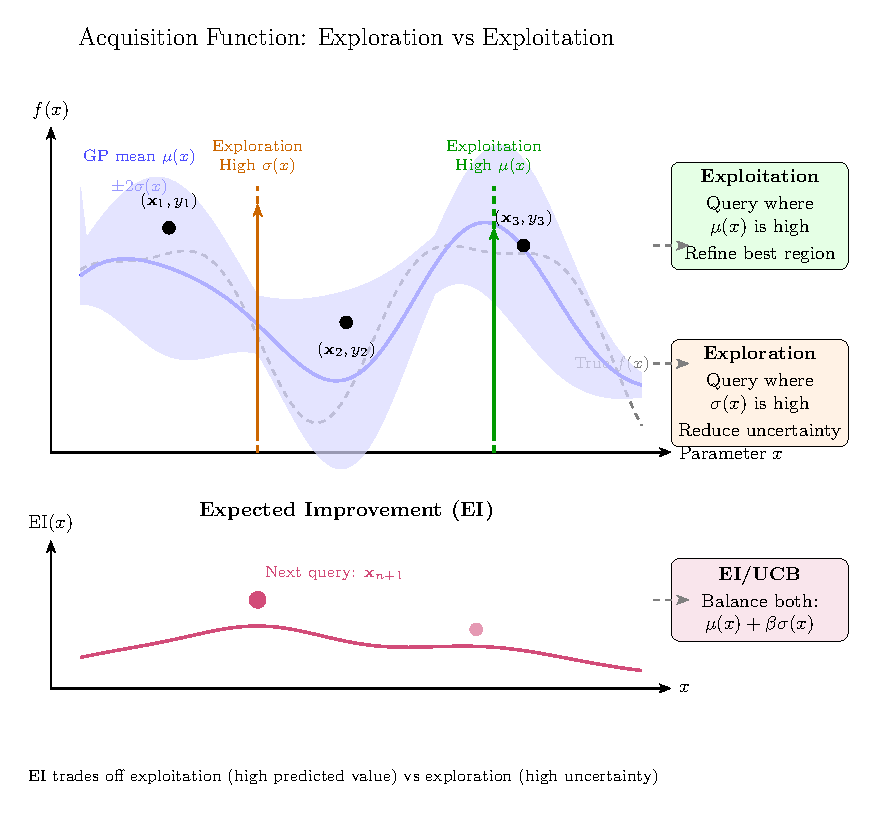
\includegraphics[width=0.95\textwidth]{figures/ch03_fig3_exploration_exploitation.pdf}
\caption{Exploration versus exploitation in Bayesian optimization. The top panel shows a Gaussian process surrogate model with mean prediction (solid line) and uncertainty band (shaded region). Observed data points reduce uncertainty locally. Exploitation favors regions with high predicted values, while exploration targets regions with high uncertainty. The bottom panel shows the Expected Improvement acquisition function, which combines both objectives to select the next query point. The acquisition function peaks in regions that offer either high predicted performance or substantial uncertainty reduction.}
\label{fig:exploration_exploitation}
\end{figure}

\subsection{Comparative Analysis of Optimization Algorithms}
\label{subsec:algorithm_comparison}

The selection of an optimization algorithm depends critically on the problem characteristics, including dimensionality, budget constraints, presence of categorical parameters, and computational resources available for surrogate model fitting. Table~\ref{tab:algorithm_comparison} provides a comprehensive comparison of leading algorithms across these dimensions.

\begin{table}[htbp]
\centering
\caption{Comparison of Optimization Algorithms for Expensive Black-Box Problems}
\label{tab:algorithm_comparison}
\renewcommand{\arraystretch}{1.3}
\begin{tabular}{|p{2.2cm}|p{1.8cm}|p{1.5cm}|p{2.0cm}|p{2.2cm}|p{2.5cm}|}
\hline
\textbf{Algorithm} & \textbf{Sample Efficiency} & \textbf{Max Dims} & \textbf{Handles Categorical} & \textbf{Parallelization} & \textbf{Best Use Case} \\
\hline
GP-BO (EI/UCB) & Very High & 10--20 & Limited & Batch acquisition & Low-dim continuous \\
\hline
TPE & High & 50--100 & Native & Independent sampling & Mixed spaces \\
\hline
SMAC & High & 100+ & Native & Racing & Algorithm config \\
\hline
TuRBO & Very High & 20--50 & Limited & Trust regions & High-dim continuous \\
\hline
BOHB & High & 50+ & Native & Parallel brackets & Multi-fidelity \\
\hline
CMA-ES & Moderate & 100+ & No & Population & Continuous only \\
\hline
PBT & Moderate & 20--50 & Limited & Highly parallel & Schedule learning \\
\hline
PPO & Low & Unlimited & Yes & Parallel envs & Dense rewards \\
\hline
SAC & Low--Moderate & Unlimited & Limited & Limited & Continuous control \\
\hline
\end{tabular}
\end{table}

Gaussian Process Bayesian Optimization with Expected Improvement or Upper Confidence Bound acquisition functions represents the gold standard for sample efficiency in low-dimensional continuous optimization. The cubic scaling of exact Gaussian process inference limits applicability to approximately twenty dimensions and a few thousand observations, though sparse approximations and local models extend this range. For generator optimization problems with fewer than twenty continuous parameters, this approach offers the best expected performance per evaluation.

The Tree-Parzen Estimator relaxes the dimensionality constraints of Gaussian processes while maintaining strong sample efficiency. By modeling the density of configurations separately for those above and below a performance threshold, TPE avoids the computational burden of full joint modeling. The kernel density estimation approach handles mixed continuous and categorical parameters naturally, making TPE particularly suitable for generator optimization where parameters may include discrete choices such as augmentation types or continuous values such as noise levels.

Sequential Model-based Algorithm Configuration extends Bayesian optimization with random forests as the surrogate model, offering superior handling of categorical and conditional parameters. The random forest surrogate scales linearly with the number of observations and handles high cardinality categorical variables without explicit encoding. SMAC's racing mechanism provides additional efficiency by early-stopping clearly inferior configurations, making it well-suited for scenarios where partial evaluations provide informative signals.

Trust Region Bayesian Optimization addresses the curse of dimensionality through a local modeling approach that maintains multiple trust regions around promising configurations. Rather than building a single global surrogate model, TuRBO fits local Gaussian process models within each trust region and adapts region sizes based on optimization progress. Successful evaluations expand the trust region to enable broader exploration, while failures contract it to focus on exploitation. This approach achieves state-of-the-art performance on optimization benchmarks with up to fifty dimensions.

Covariance Matrix Adaptation Evolution Strategy provides a gradient-free optimization method based on evolving a multivariate normal sampling distribution. CMA-ES adapts both the mean and covariance matrix of the distribution based on the ranking of sampled solutions, enabling automatic discovery of appropriate step sizes and parameter correlations. While less sample-efficient than Bayesian methods for very expensive objectives, CMA-ES offers robust performance across a wide range of problem types and scales well to high dimensions. The algorithm is particularly effective when parallel evaluation of population members is possible.


\section{BOHB: Bayesian Optimization with Hyperband}
\label{sec:bohb}

Bayesian Optimization with Hyperband represents a principled integration of Bayesian optimization's sample efficiency with Hyperband's multi-fidelity scheduling. This combination addresses a fundamental limitation of standard Bayesian optimization: the assumption that all function evaluations have equal cost. In practice, many optimization problems admit cheap approximations to the full objective, such as training with fewer epochs or evaluating on a subset of the data. BOHB exploits this structure to dramatically accelerate optimization by allocating resources adaptively based on early performance signals.

\subsection{Theoretical Foundations}
\label{subsec:bohb_theory}

The theoretical justification for BOHB rests on the observation that performance rankings of configurations often stabilize before full evaluation completes. If a configuration performs poorly with a small computational budget, it is unlikely to become optimal with additional resources. This observation motivates early stopping of unpromising configurations to redirect resources toward more promising alternatives. Hyperband formalizes this intuition through successive halving, progressively eliminating the worst-performing fraction of configurations at each stage.

The integration with Bayesian optimization addresses Hyperband's primary weakness: random configuration sampling. While Hyperband efficiently allocates resources among sampled configurations, the quality of the initial sample critically determines final performance. By replacing random sampling with Tree-Parzen Estimator-guided sampling, BOHB combines the adaptive resource allocation of Hyperband with the informed exploration of Bayesian optimization.

The theoretical analysis of BOHB establishes regret bounds that interpolate between pure Bayesian optimization and pure Hyperband depending on the correlation structure between cheap and expensive evaluations. When cheap evaluations are highly predictive of expensive ones, BOHB achieves near-optimal sample complexity with respect to the cheap fidelity while maintaining guarantees with respect to the true objective. This formal analysis provides guidance on when multi-fidelity optimization offers substantial benefits versus when standard Bayesian optimization suffices.

\subsection{Tree-Parzen Estimator Sampler}
\label{subsec:tpe}

The Tree-Parzen Estimator provides the probabilistic model underlying BOHB's configuration sampling. Unlike Gaussian process-based Bayesian optimization, which models the objective function directly as $p(y | \mathbf{x})$, TPE models the inverse relationship $p(\mathbf{x} | y)$ by separately estimating densities for good and bad configurations. This reformulation offers computational advantages and natural handling of complex parameter spaces.

The algorithm partitions observed configurations into two groups based on a quantile threshold $\gamma$, typically set to 0.15 or 0.25. Configurations with objective values in the top $\gamma$ quantile form the good set $\mathcal{D}_\ell$, while the remainder form the bad set $\mathcal{D}_g$. Kernel density estimation constructs probability density functions $\ell(\mathbf{x})$ and $g(\mathbf{x})$ over the parameter space for each group. The acquisition function then evaluates configurations based on the density ratio, preferring regions where good configurations are dense relative to bad ones.

For continuous parameters, TPE employs truncated Gaussian kernels centered on observed values, with bandwidth adapted to the local density of observations. The truncation ensures that sampled configurations respect parameter bounds. For categorical parameters, TPE uses a weighted mixture model that places probability mass on observed categories proportionally to their frequency in the good set, with a small uniform component for exploration.

The Expected Improvement acquisition function under the TPE model takes a particularly simple form. Rather than requiring numerical integration as in Gaussian process-based methods, the TPE formulation yields the closed-form expression:

\begin{equation}
\text{EI}(\mathbf{x}) \propto \frac{\gamma + (1-\gamma) \cdot g(\mathbf{x})/\ell(\mathbf{x})}{1}
\end{equation}

Maximizing Expected Improvement thus reduces to maximizing $\ell(\mathbf{x})/g(\mathbf{x})$, which is achieved by sampling candidates from $\ell(\mathbf{x})$ and evaluating the ratio. This procedure is computationally efficient and scales gracefully to high dimensions through the factorized density model.

\subsection{Integration with Successive Halving}
\label{subsec:successive_halving}

Successive halving provides the resource allocation mechanism within BOHB. Given a set of configurations and a budget constraint, successive halving evaluates all configurations at the minimum fidelity, eliminates the worst-performing fraction, and repeats with increased fidelity for survivors until only one configuration remains or the maximum fidelity is reached. This geometric progression of resources ensures that promising configurations receive exponentially more evaluation time than unpromising ones.

The key parameters governing successive halving are the minimum and maximum fidelities $r_{\min}$ and $r_{\max}$, the reduction factor $\eta$ (typically 3), and the bracket structure determining how many configurations to sample initially. Hyperband addresses the exploration-exploitation tradeoff in choosing the initial sample size by running multiple brackets in parallel, ranging from aggressive exploration with many configurations at low fidelity to conservative exploitation with few configurations at high fidelity.

BOHB modifies standard Hyperband by replacing random sampling with TPE-guided sampling within each bracket. As evaluations complete across brackets, the TPE model incorporates results from all fidelities, enabling transfer of information between cheap and expensive evaluations. This shared modeling allows insights gained from low-fidelity evaluations to immediately influence sampling at high fidelities, accelerating convergence.

Algorithm~\ref{alg:bohb} presents the complete BOHB procedure, highlighting the interaction between Hyperband's bracket structure and TPE's probabilistic sampling.

\begin{algorithm}[htbp]
\caption{Bayesian Optimization with Hyperband (BOHB)}
\label{alg:bohb}
\begin{algorithmic}[1]
\Require Maximum budget $R$, minimum budget $r$, reduction factor $\eta$, quantile $\gamma$
\Ensure Best configuration $\mathbf{x}^*$ and corresponding objective value $y^*$
\State $s_{\max} \gets \lfloor \log_\eta(R/r) \rfloor$
\State $B \gets (s_{\max} + 1) \cdot R$ \Comment{Total budget per Hyperband round}
\State Initialize observation history $\mathcal{H} \gets \emptyset$
\State Initialize TPE models $\ell(\cdot), g(\cdot)$
\For{each Hyperband iteration}
    \For{$s \in \{s_{\max}, s_{\max}-1, \ldots, 0\}$} \Comment{Bracket loop}
        \State $n \gets \lceil \frac{B}{R} \cdot \frac{\eta^s}{s+1} \rceil$ \Comment{Initial configurations}
        \State $r_0 \gets R \cdot \eta^{-s}$ \Comment{Initial budget per config}
        \If{$|\mathcal{H}| < n_{\text{init}}$}
            \State Sample $n$ configurations uniformly at random: $\mathcal{T} \gets \{\mathbf{x}_1, \ldots, \mathbf{x}_n\}$
        \Else
            \State Fit TPE models $\ell(\cdot), g(\cdot)$ from $\mathcal{H}$ using quantile $\gamma$
            \State Sample $n$ configurations from $\ell(\cdot)$ maximizing $\ell(\mathbf{x})/g(\mathbf{x})$: $\mathcal{T} \gets \{\mathbf{x}_1, \ldots, \mathbf{x}_n\}$
        \EndIf
        \For{$i \in \{0, 1, \ldots, s\}$} \Comment{Successive halving rounds}
            \State $n_i \gets \lfloor n \cdot \eta^{-i} \rfloor$
            \State $r_i \gets r_0 \cdot \eta^i$
            \State Evaluate $\mathcal{T}$ with budget $r_i$: $\{y_{\mathbf{x}} : \mathbf{x} \in \mathcal{T}\}$
            \State Update history: $\mathcal{H} \gets \mathcal{H} \cup \{(\mathbf{x}, y_{\mathbf{x}}, r_i) : \mathbf{x} \in \mathcal{T}\}$
            \State Retain top $\lfloor n_i / \eta \rfloor$ configurations: $\mathcal{T} \gets \text{top}_k(\mathcal{T}, \lfloor n_i / \eta \rfloor)$
        \EndFor
    \EndFor
\EndFor
\State \Return $\mathbf{x}^* \gets \arg\min_{\mathbf{x} \in \mathcal{H}_{r=R}} y_{\mathbf{x}}$
\end{algorithmic}
\end{algorithm}

Figure~\ref{fig:bohb_diagram} provides a visual representation of the BOHB algorithm, illustrating how the Tree-Parzen Estimator guides configuration sampling while successive halving progressively eliminates underperforming configurations across multiple fidelity levels.

\begin{figure}[htbp]
\centering
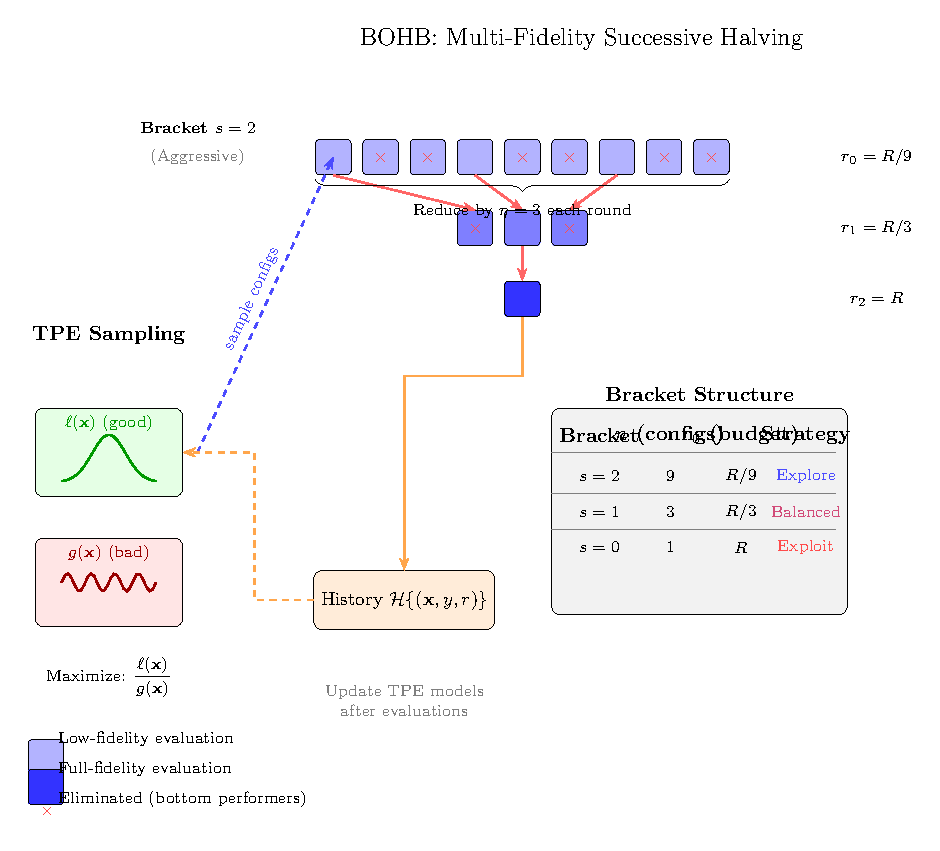
\includegraphics[width=0.95\textwidth]{figures/ch03_fig2_bohb.pdf}
\caption{BOHB algorithm overview showing the integration of TPE-guided sampling with successive halving. The bracket structure (shown for $s=2$) demonstrates how configurations are progressively evaluated at increasing fidelity levels, with the worst performers eliminated at each round. The TPE sampler models the density of good configurations $\ell(\mathbf{x})$ versus bad configurations $g(\mathbf{x})$, maximizing their ratio to propose promising new configurations. The history $\mathcal{H}$ accumulates results from all fidelity levels to continuously improve the surrogate model.}
\label{fig:bohb_diagram}
\end{figure}

\subsection{Theoretical Guarantees and Convergence}
\label{subsec:bohb_guarantees}

The theoretical analysis of BOHB provides convergence guarantees under reasonable assumptions on the relationship between low-fidelity and high-fidelity evaluations. Let $f_r(\mathbf{x})$ denote the objective at fidelity $r$ and $f_R(\mathbf{x})$ denote the objective at maximum fidelity. The key assumption is that the ranking induced by $f_r$ over configurations is partially preserved in $f_R$, formalized through bounds on the probability that the true optimum is eliminated at low fidelity.

Under these assumptions, BOHB achieves a regret bound that depends on the effective dimensionality of the parameter space and the correlation between fidelities. When correlations are strong, BOHB's regret approaches that of an oracle with access to the full fidelity evaluation at cost equal to the minimum fidelity. When correlations are weak, BOHB gracefully degrades to standard Hyperband performance with the additional overhead of TPE model fitting.

The practical implication of these guarantees is that BOHB provides robustness across a range of problem characteristics. When multi-fidelity structure is exploitable, BOHB automatically discovers and leverages this structure. When such structure is absent, BOHB remains competitive with single-fidelity methods through the quality of its configuration sampling.


\section{Population-Based Training}
\label{sec:pbt}

Population-Based Training provides an alternative paradigm for hyperparameter optimization that combines the parallelism of random search with the adaptivity of sequential optimization. Rather than optimizing hyperparameters before training begins, PBT optimizes them during training by maintaining a population of agents that share information through periodic exploitation and exploration operations. This online approach naturally discovers hyperparameter schedules rather than fixed values, offering potential advantages for problems where optimal hyperparameters change over the course of optimization.

\subsection{Algorithm Description}
\label{subsec:pbt_algorithm}

Population-Based Training maintains a population of $N$ agents, each with its own model parameters $\theta_i$ and hyperparameters $h_i$. Agents train independently for a fixed interval, after which they evaluate performance on a validation metric. Low-performing agents exploit high-performing ones by copying their model parameters and hyperparameters, then explore by perturbing the copied hyperparameters. This process repeats throughout training, enabling the population to collectively discover effective hyperparameter schedules.

The exploitation step implements a form of truncation selection. Each agent compares its performance to the population and, if in the bottom fraction (typically 20\%), selects a replacement from the top fraction. The selection may be uniform among top performers or weighted by performance. After exploitation, the agent's model parameters are replaced with those of the selected parent, providing a warm start for continued training.

The exploration step perturbs hyperparameters of agents that have just exploited. Perturbations may be multiplicative (scaling by factors such as 0.8 or 1.2), additive (adding noise from a specified distribution), or resampling from prior distributions. The perturbation scheme should be matched to the hyperparameter types and scales, with multiplicative perturbations typically preferred for learning rates and regularization strengths.

Algorithm~\ref{alg:pbt} provides a detailed specification of the Population-Based Training procedure.

\begin{algorithm}[htbp]
\caption{Population-Based Training (PBT)}
\label{alg:pbt}
\begin{algorithmic}[1]
\Require Population size $N$, exploitation fraction $\rho$, perturbation factors $\mathcal{P}$
\Ensure Trained models $\{\theta_i\}_{i=1}^N$ with discovered schedules
\State Initialize population $\{(\theta_i, h_i)\}_{i=1}^N$ with random hyperparameters
\State Initialize step counters $\{t_i \gets 0\}_{i=1}^N$
\While{not converged}
    \For{each agent $i \in \{1, \ldots, N\}$ in parallel}
        \State Train for $\Delta t$ steps: $\theta_i \gets \text{Train}(\theta_i, h_i, \Delta t)$
        \State $t_i \gets t_i + \Delta t$
        \State Evaluate performance: $p_i \gets \text{Evaluate}(\theta_i)$
    \EndFor
    \State Compute performance ranking of population
    \For{each agent $i$ with $p_i$ in bottom $\rho$ fraction}
        \State \textbf{Exploit:} Select parent $j$ from top $\rho$ fraction
        \State Copy parameters: $\theta_i \gets \theta_j$
        \State Copy hyperparameters: $h_i \gets h_j$
        \State \textbf{Explore:} Perturb hyperparameters
        \For{each hyperparameter $h_i^{(k)}$}
            \State Sample perturbation $\delta \sim \mathcal{P}$
            \State Apply: $h_i^{(k)} \gets h_i^{(k)} \cdot \delta$ \Comment{or additive}
        \EndFor
    \EndFor
\EndWhile
\State \Return $\{\theta_i\}_{i=1}^N$
\end{algorithmic}
\end{algorithm}

\subsection{Discovering Parameter Schedules}
\label{subsec:pbt_schedules}

A distinguishing feature of Population-Based Training is its ability to discover hyperparameter schedules without explicit parameterization. Because hyperparameters are adapted during training, the sequence of values encountered by agents that eventually achieve high performance constitutes an implicitly learned schedule. Post-hoc analysis of these trajectories reveals patterns that may generalize to future training runs.

The schedule discovery property is particularly valuable for learning rate optimization, where the optimal value typically decreases over training. Traditional approaches require specifying a schedule a priori, such as exponential decay or cosine annealing, with parameters that must themselves be tuned. PBT discovers effective schedules automatically, often finding non-monotonic patterns that outperform standard schedules.

Beyond learning rate, PBT has discovered effective schedules for regularization strength, data augmentation intensity, and exploration parameters in reinforcement learning. In each case, the optimal trajectory depends on the current state of training in ways that are difficult to specify analytically but emerge naturally from the population dynamics.

\subsection{Extensions: GPBT and IPBT}
\label{subsec:pbt_extensions}

Guided Population-Based Training addresses a limitation of standard PBT: the random exploration step may require many generations to discover beneficial hyperparameter changes. GPBT replaces random perturbation with surrogate model-guided search, using a Gaussian process or random forest to model the relationship between hyperparameters and performance given the current training state. This guidance accelerates discovery of effective hyperparameters while maintaining the online adaptation property.

Importance-Weighted Population-Based Training modifies the exploitation mechanism to account for the relative difficulty of different training stages. Rather than uniform exploitation throughout training, IPBT adjusts the exploitation frequency and intensity based on the marginal value of hyperparameter adaptation at each stage. Early in training, when the landscape changes rapidly, frequent exploitation is valuable. Later, when the landscape stabilizes, exploitation overhead may outweigh benefits.

These extensions share the goal of improving sample efficiency while preserving PBT's core advantages. GPBT reduces the number of generations required to discover effective schedules by replacing random exploration with informed search. IPBT reduces computational overhead by adapting exploitation frequency to the current training regime. Both approaches have demonstrated improvements over standard PBT on benchmark tasks.

\subsection{When to Prefer PBT over BOHB}
\label{subsec:pbt_vs_bohb}

The choice between Population-Based Training and BOHB depends on several problem characteristics. PBT offers advantages when hyperparameters should vary during optimization, when massively parallel evaluation is available, and when the optimization horizon is long enough for population dynamics to operate effectively. BOHB offers advantages when hyperparameters are fixed during optimization, when sequential evaluation is acceptable, and when the budget is too limited for population-based approaches.

For generator parameter optimization, the appropriate choice depends on whether parameters should remain fixed throughout YOLO training or adapt as training progresses. If the generator runs once at the beginning of each training run, producing a fixed dataset, then BOHB's sample efficiency makes it the preferred choice. If the generator could be integrated into the training loop, producing new samples adaptively, then PBT's schedule discovery becomes relevant.

Computational considerations also influence the choice. PBT requires maintaining $N$ parallel training runs throughout optimization, with $N$ typically ranging from 10 to 100. For expensive training procedures, this requirement may exceed available resources. BOHB's sequential nature with optional parallelization over brackets provides more flexibility in resource allocation.


\section{Continuous Control RL Methods}
\label{sec:continuous_control}

While Bayesian optimization methods offer superior sample efficiency for expensive black-box optimization, reinforcement learning algorithms designed for continuous control remain relevant in specific scenarios. When the optimization horizon extends to allow thousands of evaluations, when the action space has special structure that policies can exploit, or when transfer learning from related tasks is possible, modern actor-critic algorithms may become competitive. This section provides detailed treatment of Soft Actor-Critic and Twin Delayed DDPG, the leading algorithms for continuous control.

\subsection{Soft Actor-Critic}
\label{subsec:sac}

Soft Actor-Critic represents the state of the art in off-policy reinforcement learning for continuous action spaces. The algorithm combines three key innovations: an actor-critic architecture with separate policy and value function approximators, off-policy learning through experience replay, and maximum entropy regularization that encourages exploration and improves robustness.

The maximum entropy framework augments the standard reinforcement learning objective with an entropy bonus, yielding the maximum entropy objective:

\begin{equation}
J(\pi) = \sum_{t=0}^{T} \mathbb{E}_{(\mathbf{s}_t, \mathbf{a}_t) \sim \rho_\pi} \left[ r(\mathbf{s}_t, \mathbf{a}_t) + \alpha \mathcal{H}(\pi(\cdot | \mathbf{s}_t)) \right]
\end{equation}

where $\mathcal{H}(\pi(\cdot | \mathbf{s})) = -\mathbb{E}_{\mathbf{a} \sim \pi}[\log \pi(\mathbf{a} | \mathbf{s})]$ is the entropy of the policy at state $\mathbf{s}$, and $\alpha$ is a temperature parameter controlling the relative importance of entropy versus reward. Higher entropy policies spread probability mass across actions, encouraging exploration and preventing premature convergence to deterministic solutions.

The practical benefits of maximum entropy regularization extend beyond exploration. Policies with higher entropy are more robust to perturbations in the environment dynamics, as they maintain probability mass on alternative actions. This robustness property is particularly valuable in transfer settings, where policies trained in simulation must generalize to real-world conditions that differ from training.

Soft Actor-Critic employs two soft Q-functions to address overestimation bias, taking the minimum of their predictions when computing target values. The soft Q-function is defined as:

\begin{equation}
Q^\pi(\mathbf{s}_t, \mathbf{a}_t) = r(\mathbf{s}_t, \mathbf{a}_t) + \gamma \mathbb{E}_{\mathbf{s}_{t+1} \sim p} \left[ V^\pi(\mathbf{s}_{t+1}) \right]
\end{equation}

where the soft value function incorporates the entropy bonus:

\begin{equation}
V^\pi(\mathbf{s}) = \mathbb{E}_{\mathbf{a} \sim \pi} \left[ Q^\pi(\mathbf{s}, \mathbf{a}) - \alpha \log \pi(\mathbf{a} | \mathbf{s}) \right]
\end{equation}

The policy is represented as a Gaussian with state-dependent mean and variance, parameterized by a neural network. Actions are sampled using the reparameterization trick, enabling gradient-based optimization of the policy through the Q-function:

\begin{equation}
\mathbf{a}_t = \mu_\phi(\mathbf{s}_t) + \sigma_\phi(\mathbf{s}_t) \odot \epsilon, \quad \epsilon \sim \mathcal{N}(0, I)
\end{equation}

The temperature parameter $\alpha$ may be fixed or learned automatically. Automatic temperature adjustment optimizes $\alpha$ to maintain a target entropy level, adapting the exploration-exploitation tradeoff to the current policy's behavior. This automatic tuning eliminates a sensitive hyperparameter and improves performance across diverse tasks.

\begin{algorithm}[htbp]
\caption{Soft Actor-Critic (SAC)}
\label{alg:sac}
\begin{algorithmic}[1]
\Require Learning rates $\lambda_Q, \lambda_\pi, \lambda_\alpha$, target entropy $\bar{\mathcal{H}}$, discount $\gamma$, soft update rate $\tau$
\Ensure Trained policy $\pi_\phi$
\State Initialize Q-networks $Q_{\theta_1}, Q_{\theta_2}$ and target networks $Q_{\bar{\theta}_1}, Q_{\bar{\theta}_2}$
\State Initialize policy network $\pi_\phi$ and temperature $\alpha$
\State Initialize replay buffer $\mathcal{D} \gets \emptyset$
\For{each iteration}
    \For{each environment step}
        \State Sample action: $\mathbf{a}_t \sim \pi_\phi(\cdot | \mathbf{s}_t)$
        \State Execute action, observe $\mathbf{s}_{t+1}, r_t$
        \State Store transition: $\mathcal{D} \gets \mathcal{D} \cup \{(\mathbf{s}_t, \mathbf{a}_t, r_t, \mathbf{s}_{t+1})\}$
    \EndFor
    \For{each gradient step}
        \State Sample minibatch $\mathcal{B} = \{(\mathbf{s}, \mathbf{a}, r, \mathbf{s}')\}$ from $\mathcal{D}$
        \State Sample next actions: $\tilde{\mathbf{a}}' \sim \pi_\phi(\cdot | \mathbf{s}')$
        \State Compute target Q-value:
        \State \quad $y = r + \gamma \left( \min_{j=1,2} Q_{\bar{\theta}_j}(\mathbf{s}', \tilde{\mathbf{a}}') - \alpha \log \pi_\phi(\tilde{\mathbf{a}}' | \mathbf{s}') \right)$
        \State Update Q-functions:
        \State \quad $\theta_i \gets \theta_i - \lambda_Q \nabla_{\theta_i} \frac{1}{|\mathcal{B}|} \sum_{(\mathbf{s},\mathbf{a},r,\mathbf{s}')} (Q_{\theta_i}(\mathbf{s}, \mathbf{a}) - y)^2$
        \State Sample actions for policy update: $\tilde{\mathbf{a}} \sim \pi_\phi(\cdot | \mathbf{s})$
        \State Update policy:
        \State \quad $\phi \gets \phi - \lambda_\pi \nabla_\phi \frac{1}{|\mathcal{B}|} \sum_\mathbf{s} \left( \alpha \log \pi_\phi(\tilde{\mathbf{a}} | \mathbf{s}) - \min_{j} Q_{\theta_j}(\mathbf{s}, \tilde{\mathbf{a}}) \right)$
        \State Update temperature:
        \State \quad $\alpha \gets \alpha - \lambda_\alpha \nabla_\alpha \frac{1}{|\mathcal{B}|} \sum_\mathbf{s} \left( -\alpha \log \pi_\phi(\tilde{\mathbf{a}} | \mathbf{s}) - \alpha \bar{\mathcal{H}} \right)$
        \State Soft update targets: $\bar{\theta}_i \gets \tau \theta_i + (1-\tau) \bar{\theta}_i$
    \EndFor
\EndFor
\State \Return $\pi_\phi$
\end{algorithmic}
\end{algorithm}

\subsection{Twin Delayed DDPG}
\label{subsec:td3}

Twin Delayed Deep Deterministic Policy Gradient builds on the DDPG algorithm by addressing three sources of instability: overestimation bias in the Q-function, high variance updates from stale critic estimates, and sensitivity to hyperparameters. The resulting algorithm achieves competitive performance with SAC while using a deterministic policy, avoiding the entropy computation and stochastic policy optimization of SAC.

The twin Q-functions of TD3 address overestimation through the clipped double Q-learning update. Target values are computed using the minimum of two Q-function predictions:

\begin{equation}
y = r + \gamma \min_{j=1,2} Q_{\bar{\theta}_j}(\mathbf{s}', \pi_{\bar{\phi}}(\mathbf{s}'))
\end{equation}

This pessimistic estimate counteracts the optimistic bias that arises from maximizing over noisy Q-value estimates.

Delayed policy updates reduce variance by updating the policy less frequently than the Q-functions, typically once per two Q-function updates. This allows the Q-functions to stabilize before influencing the policy, reducing the propagation of errors from critic to actor.

Target policy smoothing adds noise to target actions, regularizing the Q-function to be smooth with respect to actions:

\begin{equation}
\tilde{\mathbf{a}}' = \pi_{\bar{\phi}}(\mathbf{s}') + \epsilon, \quad \epsilon \sim \text{clip}(\mathcal{N}(0, \sigma), -c, c)
\end{equation}

This smoothing prevents the policy from exploiting narrow peaks in the Q-function landscape that may not correspond to genuinely high-value actions.

\subsection{Maximum Entropy Framework}
\label{subsec:max_entropy}

The maximum entropy framework provides theoretical grounding for the exploration bonuses used in SAC and related algorithms. By treating the reinforcement learning problem as inference in a probabilistic graphical model, maximum entropy methods derive principled objectives that balance reward maximization with maintaining uncertainty about the optimal solution.

The soft Bellman equation generalizes the standard Bellman equation to incorporate entropy:

\begin{equation}
Q^\pi(\mathbf{s}, \mathbf{a}) = r(\mathbf{s}, \mathbf{a}) + \gamma \mathbb{E}_{\mathbf{s}'} \left[ \mathbb{E}_{\mathbf{a}' \sim \pi} \left[ Q^\pi(\mathbf{s}', \mathbf{a}') - \alpha \log \pi(\mathbf{a}' | \mathbf{s}') \right] \right]
\end{equation}

The optimal policy under this framework takes the form of a Boltzmann distribution over the Q-function:

\begin{equation}
\pi^*(\mathbf{a} | \mathbf{s}) = \exp\left( \frac{1}{\alpha} \left( Q^*(\mathbf{s}, \mathbf{a}) - V^*(\mathbf{s}) \right) \right)
\end{equation}

This exponential policy form arises naturally from the variational characterization of the maximum entropy problem and connects reinforcement learning to probabilistic inference.

The benefits of maximum entropy extend to transfer and robustness. Policies with higher entropy assign non-negligible probability to suboptimal actions, enabling recovery when the environment differs from training. This property is particularly valuable for sim-to-real transfer, where simulation artifacts may have caused the policy to rely on details that do not hold in reality.

Figure~\ref{fig:policy_gradient} illustrates the flow of gradients through the policy network in actor-critic methods, highlighting the role of the reparameterization trick and entropy regularization.

\begin{figure}[htbp]
\centering
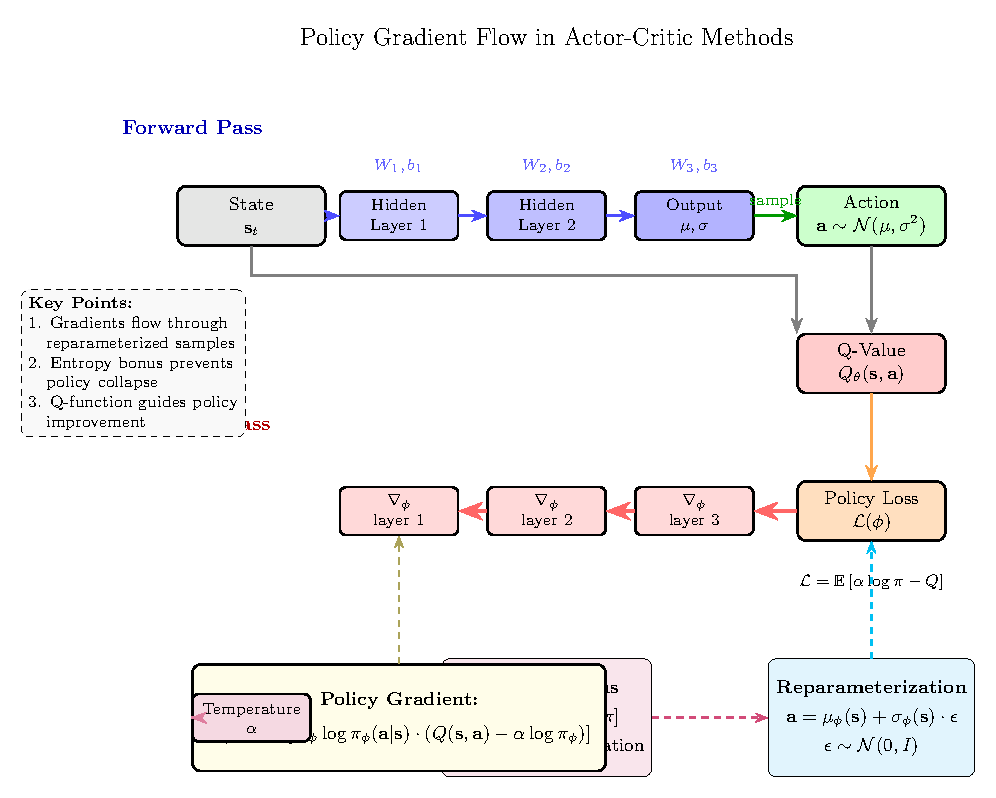
\includegraphics[width=0.95\textwidth]{figures/ch03_fig4_policy_gradient.pdf}
\caption{Policy gradient flow in actor-critic methods. The forward pass propagates state information through the policy network to produce action distributions, from which actions are sampled using the reparameterization trick. The Q-function evaluates state-action pairs to compute the policy loss. The backward pass propagates gradients through the reparameterized samples back to the policy parameters. The entropy bonus, controlled by temperature $\alpha$, encourages exploration by penalizing low-entropy policies. Key aspects include: (1) gradients flow through reparameterized samples enabling end-to-end optimization, (2) the entropy term prevents premature convergence to deterministic policies, and (3) the Q-function guides policy improvement toward high-value actions.}
\label{fig:policy_gradient}
\end{figure}

\subsection{Sample Efficiency Comparison}
\label{subsec:rl_sample_efficiency}

The sample efficiency of reinforcement learning algorithms varies substantially depending on problem characteristics and algorithmic details. Table~\ref{tab:rl_efficiency} summarizes typical sample requirements for achieving baseline performance across continuous control benchmarks.

\begin{table}[htbp]
\centering
\caption{Sample Efficiency of Continuous Control RL Algorithms}
\label{tab:rl_efficiency}
\renewcommand{\arraystretch}{1.3}
\begin{tabular}{|p{2.5cm}|p{2.0cm}|p{2.5cm}|p{2.0cm}|p{2.5cm}|}
\hline
\textbf{Algorithm} & \textbf{Samples to Baseline} & \textbf{Gradient Updates per Sample} & \textbf{Off-Policy} & \textbf{Continuous Actions} \\
\hline
PPO & 1--10M & 1 & No & Yes \\
\hline
TRPO & 1--10M & 1 & No & Yes \\
\hline
SAC & 100K--1M & 1--20 & Yes & Yes \\
\hline
TD3 & 100K--1M & 1 & Yes & Yes \\
\hline
DroQ-SAC & 10K--100K & 20 & Yes & Yes \\
\hline
REDQ & 10K--100K & 20 & Yes & Yes \\
\hline
\end{tabular}
\end{table}

Recent advances in sample-efficient reinforcement learning have reduced the gap between RL methods and Bayesian optimization. The Dropout Q-functions algorithm achieves strong performance with only tens of thousands of environment interactions through aggressive use of experience replay, performing twenty gradient updates per environment step. Similarly, Randomized Ensemble Double Q-learning maintains an ensemble of Q-functions to reduce overestimation, enabling data-efficient learning.

Despite these advances, the sample requirements of even the most efficient reinforcement learning algorithms exceed typical budgets for generator parameter optimization by one to two orders of magnitude. Reinforcement learning methods become competitive only when evaluation costs can be reduced through surrogate modeling or multi-fidelity approximation, or when prior knowledge can be transferred from related optimization tasks.


\section{State and Action Space Design}
\label{sec:state_action_design}

The design of state and action representations critically influences the performance of both reinforcement learning and Bayesian optimization methods. Effective representations compress the relevant information for decision-making while remaining tractable for function approximation or density modeling. This section examines design considerations for representing generator parameters as actions and encoding relevant state information.

\subsection{Representing Generator Parameters as Actions}
\label{subsec:parameter_actions}

Generator parameters form the natural action space for parameter optimization agents. Each configuration of the generator corresponds to a point in the action space, and the optimization objective is to find the action that maximizes downstream detection performance. The structure of this action space depends on the types and ranges of generator parameters.

Continuous parameters such as noise variance, object scale ranges, and lighting intensity map directly to bounded continuous action dimensions. The bounds should reflect physically meaningful or empirically determined limits on parameter values. Normalization of actions to a standard range, typically $[-1, 1]$ or $[0, 1]$, facilitates learning by ensuring that all dimensions contribute comparably to network activations.

The choice of parameterization affects optimization difficulty. For example, representing a scale range as (minimum, maximum) creates constraints that the minimum must not exceed the maximum. Alternative parameterizations such as (center, width) or (minimum, width) may simplify the feasible region, though they change the meaning of uniform sampling over the space.

\subsection{Continuous versus Discrete Parameter Handling}
\label{subsec:continuous_discrete}

Many generator configurations involve both continuous and discrete parameters. Discrete parameters include categorical choices such as augmentation types, texture categories, or background scenes, as well as integer parameters such as the number of objects per image. Handling mixed continuous-discrete spaces requires either specialized algorithms or careful encoding strategies.

One-hot encoding transforms categorical parameters into binary vectors, expanding the action space dimensionality but enabling application of continuous optimization methods. A categorical parameter with $k$ categories becomes $k$ binary dimensions with the constraint that exactly one is active. Relaxation approaches treat these dimensions as continuous probabilities, sampling from the resulting categorical distribution or taking the argmax for evaluation.

Ordinal parameters with natural ordering, such as discretized intensity levels, may be treated as continuous and rounded to the nearest valid value. This approach preserves gradient information through the rounding operation, enabling gradient-based optimization. However, rounding can create plateaus in the objective landscape where small parameter changes produce no change in the discrete value.

Tree-structured parameter spaces arise when some parameters are conditional on others. For example, the parameters of a specific augmentation are only relevant if that augmentation is enabled. Modeling these dependencies explicitly improves sample efficiency by avoiding evaluation of configurations with irrelevant parameters set to arbitrary values. The Tree-Parzen Estimator and SMAC handle conditional spaces natively, while standard Gaussian process models require explicit encoding.

\subsection{Hierarchical Action Spaces}
\label{subsec:hierarchical_actions}

Hierarchical action spaces decompose the full configuration into groups that can be optimized at different granularities or timescales. This decomposition reflects structure in the optimization problem, where some parameters may interact strongly within groups but weakly across groups. Exploiting this structure improves scalability to high-dimensional configuration spaces.

A two-level hierarchy might distinguish between coarse parameters that dramatically affect data distribution, such as object categories and scene types, and fine parameters that provide detailed control, such as exact placement distributions and noise levels. The outer level searches over coarse configurations while the inner level optimizes fine parameters conditional on the coarse choice. This decomposition reduces effective dimensionality at each level while preserving the ability to optimize the full space.

Temporal hierarchies adapt parameters at different frequencies during training. Slowly-varying parameters such as the overall difficulty of generated scenes might be adjusted every few epochs, while rapidly-varying parameters such as specific augmentation probabilities might change every batch. This temporal structure aligns with Population-Based Training's schedule discovery capability.

\subsection{State Representation}
\label{subsec:state_representation}

While pure black-box optimization treats each evaluation independently, incorporating state information can improve optimization efficiency by enabling transfer of knowledge across the optimization trajectory. Relevant state information includes the current parameter configuration, the history of previous evaluations, and summary statistics of the current training run.

The current parameter configuration provides context for value function learning in reinforcement learning approaches. Rather than learning a single optimal configuration, the value function can learn a landscape over configurations, enabling generalization and accelerating exploration. This state representation is implicit in Bayesian optimization through the surrogate model but requires explicit design in policy-based methods.

Historical performance metrics summarize the optimization trajectory, indicating which regions have been explored and how performance has evolved. Including this history enables policies to condition decisions on past experience, implementing forms of adaptive exploration. Encoding history efficiently requires compression, such as maintaining running statistics or using recurrent architectures.

Training dynamics metrics such as current loss, gradient norms, or validation performance provide real-time signals that may inform parameter adjustment before full evaluation completes. These signals enable early stopping of unpromising configurations or adaptive parameter adjustment during training, connecting to the multi-fidelity optimization framework.

Table~\ref{tab:action_space} summarizes typical action space dimensions for generator parameter optimization.

\begin{table}[htbp]
\centering
\caption{Action Space Dimensions for Generator Parameter Optimization}
\label{tab:action_space}
\renewcommand{\arraystretch}{1.3}
\begin{tabular}{|p{3.5cm}|p{2.0cm}|p{2.5cm}|p{4.0cm}|}
\hline
\textbf{Parameter Category} & \textbf{Type} & \textbf{Dimensions} & \textbf{Example Parameters} \\
\hline
Object placement & Continuous & 4--8 & Position range, scale range, rotation range \\
\hline
Lighting conditions & Continuous & 3--6 & Intensity, direction, color temperature \\
\hline
Scene composition & Mixed & 5--10 & Object count, clutter level, occlusion rate \\
\hline
Noise and artifacts & Continuous & 2--4 & Gaussian noise, motion blur, compression \\
\hline
Augmentation selection & Categorical & 10--20 & Flip, crop, color jitter probabilities \\
\hline
Domain parameters & Mixed & 5--15 & Background type, texture, weather conditions \\
\hline
\textbf{Total typical range} & Mixed & \textbf{30--60} & Full generator configuration \\
\hline
\end{tabular}
\end{table}


\section{Experience Replay and Sample Efficiency}
\label{sec:experience_replay}

Sample efficiency is paramount in expensive black-box optimization, where each evaluation may require hours of computation. This section examines techniques for maximizing the information extracted from each evaluation, including advanced experience replay strategies, transfer learning approaches, and surrogate model construction.

\subsection{Prioritized Experience Replay}
\label{subsec:per}

Prioritized Experience Replay improves sample efficiency by replaying transitions in proportion to their learning value rather than uniformly at random. Transitions with high temporal difference error indicate regions where the value function is poorly calibrated, suggesting that additional learning from these transitions would be beneficial. By focusing gradient updates on informative transitions, PER accelerates learning from limited data.

The priority of transition $i$ is defined based on its temporal difference error:

\begin{equation}
p_i = |\delta_i| + \epsilon
\end{equation}

where $\delta_i = r_i + \gamma V(\mathbf{s}'_i) - Q(\mathbf{s}_i, \mathbf{a}_i)$ is the TD error, and $\epsilon$ is a small constant ensuring non-zero probability for all transitions. The sampling probability follows a power law:

\begin{equation}
P(i) = \frac{p_i^\alpha}{\sum_k p_k^\alpha}
\end{equation}

where $\alpha$ controls the degree of prioritization, with $\alpha = 0$ recovering uniform sampling.

Non-uniform sampling introduces bias into gradient estimates, as transitions with high priority contribute disproportionately to learning. Importance sampling weights correct for this bias:

\begin{equation}
w_i = \left( \frac{1}{N \cdot P(i)} \right)^\beta
\end{equation}

where $\beta$ controls the degree of correction, typically annealed from a low initial value to 1 over training. Full correction ($\beta = 1$) eliminates bias at the cost of higher variance.

For generator parameter optimization, prioritized replay can be adapted to emphasize configurations with surprising performance, either much better or much worse than predicted by a surrogate model. This adaptation aligns the RL notion of TD error with the Bayesian optimization notion of information gain, bridging the two paradigms.

\subsection{Transfer Learning Between Optimization Runs}
\label{subsec:transfer_learning}

Transfer learning accelerates optimization by leveraging experience from related tasks. When optimizing generator parameters for multiple object detection datasets or model architectures, knowledge from previous optimization runs can warm-start new runs, reducing the number of expensive evaluations required.

The most direct form of transfer is warm-starting from previously successful configurations. Rather than initializing optimization from a default or random configuration, initialization near configurations that performed well on related tasks provides a better starting point. The effectiveness of warm-starting depends on the similarity between tasks; highly dissimilar tasks may not benefit or may even suffer from biased initialization.

Surrogate model transfer maintains the probabilistic model across optimization runs, incorporating prior observations into the posterior. Gaussian process models naturally support this through the prior mean and kernel hyperparameters, which can be set based on previous tasks. The neural network-based surrogates used in neural acquisition functions enable more flexible transfer through pre-training on historical data.

Meta-learning approaches learn to optimize across distributions of tasks, developing strategies that transfer to new tasks with minimal adaptation. Model-Agnostic Meta-Learning and related algorithms learn parameter initializations that enable rapid fine-tuning, while learned optimizers encode optimization strategies directly in neural network weights. These approaches require many source tasks for training but can dramatically accelerate optimization on target tasks.

Policy transfer in reinforcement learning involves transferring the policy network weights from source to target task. Pre-trained policies provide useful behaviors that can be fine-tuned with limited data from the target task. Successful transfer requires shared structure between source and target, such as similar action spaces and reward structures.

\subsection{Surrogate Model Construction}
\label{subsec:surrogate_models}

Surrogate models approximate the expensive objective function, enabling cheap evaluation of candidate configurations during optimization. The surrogate guides search toward promising regions while the true objective is evaluated only at selected points to update the surrogate and verify predictions.

Gaussian process surrogates provide uncertainty quantification alongside predictions, enabling principled exploration-exploitation tradeoffs through acquisition functions. The kernel function encodes assumptions about the objective's smoothness and structure, with the Mat\'ern 5/2 kernel providing a common default that allows for some non-smoothness while remaining tractable. Kernel hyperparameters are typically optimized by maximizing the marginal likelihood of observed data.

Random forest surrogates, as used in SMAC, offer scalability and native handling of categorical variables. Each tree in the forest provides a prediction, and the variance of predictions across trees serves as an uncertainty estimate. While less principled than Gaussian process uncertainty, this empirical variance captures epistemic uncertainty adequately for guiding optimization.

Neural network surrogates scale to large datasets and complex input representations, including images or sequences that characterize the optimization context. Uncertainty quantification in neural networks remains challenging, with approaches including dropout-based variational inference, ensembles, and explicit uncertainty heads. The flexibility of neural surrogates enables conditioning on rich state representations, supporting transfer learning and multi-task optimization.

The accuracy of surrogate models depends critically on the diversity of training data. Sequential optimization naturally explores the objective landscape, but early data may concentrate in suboptimal regions. Balancing exploration for surrogate improvement against exploitation for objective optimization is a central challenge, addressed through acquisition functions that account for information gain.

Figure~\ref{fig:actor_critic} illustrates the actor-critic architecture underlying SAC and related algorithms, showing the flow of information between policy, value function, and environment.

\begin{figure}[htbp]
\centering
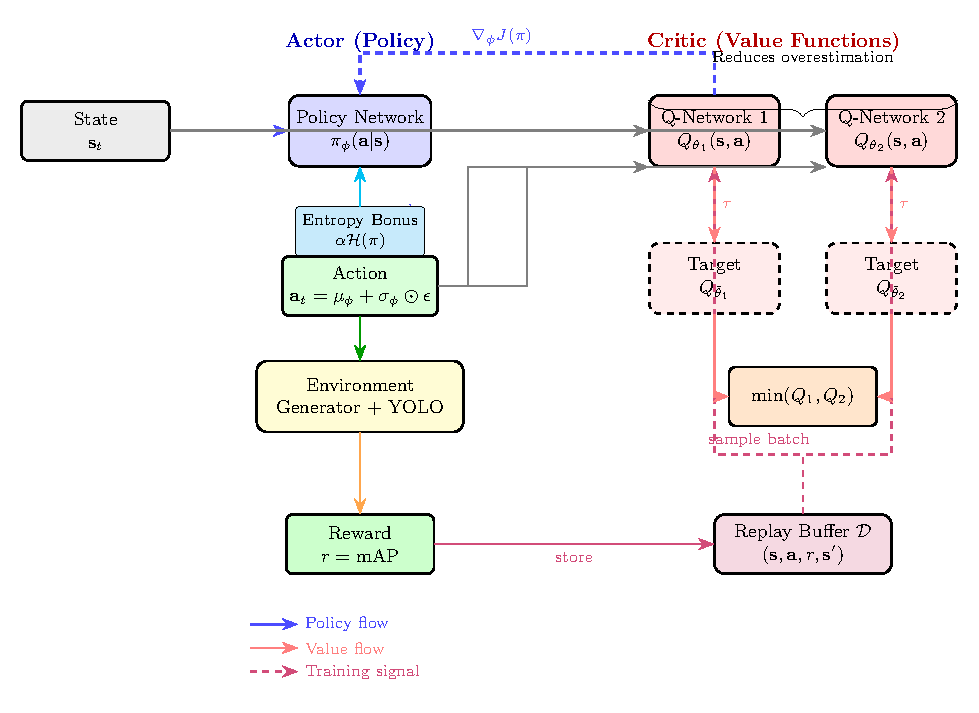
\includegraphics[width=0.95\textwidth]{figures/ch03_fig1_actor_critic.pdf}
\caption{Actor-critic architecture for generator parameter optimization. The actor network outputs parameter configurations as actions, which are evaluated through the generator and YOLO training pipeline. The twin critic networks estimate action values, with the minimum used for target computation to reduce overestimation. Soft updates transfer critic weights to target networks. The replay buffer stores transitions for off-policy learning. The entropy bonus encourages exploration and prevents premature policy collapse.}
\label{fig:actor_critic}
\end{figure}


\section{Convergence Analysis and Algorithm Selection Guidelines}
\label{sec:convergence}

The convergence properties of optimization algorithms provide theoretical guidance for algorithm selection, though practical performance depends on problem-specific factors that may not be captured by asymptotic analysis. This section summarizes convergence results and provides practical guidelines for selecting among the algorithms presented in this chapter.

\subsection{Convergence Rate Comparison}
\label{subsec:convergence_rates}

Table~\ref{tab:convergence} summarizes theoretical convergence rates for the major algorithm classes, expressed in terms of the number of function evaluations required to achieve $\epsilon$-optimal solutions.

\begin{table}[htbp]
\centering
\caption{Convergence Rates of Optimization Algorithms}
\label{tab:convergence}
\renewcommand{\arraystretch}{1.3}
\begin{tabular}{|p{2.5cm}|p{3.0cm}|p{3.0cm}|p{3.5cm}|}
\hline
\textbf{Algorithm} & \textbf{Rate} & \textbf{Assumptions} & \textbf{Notes} \\
\hline
GP-BO (EI) & $O\left(\frac{(\log n)^{d+1}}{n}\right)$ & Smooth objective, known kernel & Near-optimal for smooth functions \\
\hline
GP-BO (UCB) & $O\left(\sqrt{\frac{\gamma_n}{n}}\right)$ & Bounded RKHS norm & $\gamma_n$ is information gain \\
\hline
TPE & $O\left(\frac{1}{\sqrt{n}}\right)$ & Lipschitz objective & Dimension-independent rate \\
\hline
CMA-ES & $O\left(\frac{d}{n}\right)$ & Convex, quadratic & Linear in dimension \\
\hline
Random Search & $O\left(\frac{1}{n^{1/d}}\right)$ & Lipschitz objective & Exponential in dimension \\
\hline
Policy Gradient & $O\left(\frac{1}{\sqrt{n}}\right)$ & Smooth policy class & High variance constants \\
\hline
\end{tabular}
\end{table}

Gaussian process Bayesian optimization with Upper Confidence Bound achieves a regret bound of $O(\sqrt{\gamma_n / n})$, where $\gamma_n$ is the maximum information gain about the objective function from $n$ observations. For common kernels, $\gamma_n$ grows polylogarithmically in $n$, yielding near-optimal rates. The Expected Improvement acquisition function achieves similar rates under slightly different assumptions, with the constant factors depending on the problem-specific regularity of the objective.

Tree-Parzen Estimators achieve a dimension-independent convergence rate under Lipschitz assumptions, though the constant factors may depend exponentially on dimension in worst-case settings. The practical performance of TPE often exceeds what the worst-case analysis suggests, particularly for structured problems where only a subset of parameters significantly affects the objective.

Evolution strategies such as CMA-ES converge linearly for convex quadratic functions, with rates that scale favorably with dimension. For non-convex functions, the analysis is more complex, but empirical performance remains strong. The population-based nature of CMA-ES enables parallel evaluation, which can compensate for lower per-evaluation efficiency when parallel resources are available.

\subsection{Practical Algorithm Selection}
\label{subsec:practical_selection}

The choice of optimization algorithm for generator parameter optimization should be guided by the following considerations. First, the evaluation budget determines which algorithms are feasible. With fewer than 100 evaluations, Gaussian process Bayesian optimization with Expected Improvement provides the best expected performance, as the cubic scaling is not yet problematic and sample efficiency is paramount. With 100 to 1000 evaluations, TPE and BOHB become competitive, offering better scaling without substantial loss of efficiency. Beyond 1000 evaluations, evolutionary methods and reinforcement learning algorithms become viable, particularly when parallel evaluation is available.

Second, the parameter space structure influences algorithm suitability. Purely continuous spaces of moderate dimension favor Gaussian process methods. Mixed continuous-categorical spaces favor TPE and SMAC. Very high-dimensional spaces may require dimensionality reduction or local optimization methods such as TuRBO. Conditional parameter spaces require specialized handling available in TPE and SMAC but not standard Gaussian process implementations.

Third, the availability of multi-fidelity approximations changes the analysis. When cheap approximations to the objective are available, such as training with fewer epochs or smaller datasets, BOHB offers substantial acceleration by intelligently allocating resources across fidelity levels. Without multi-fidelity structure, BOHB reduces to standard TPE with the overhead of bracket management.

Fourth, the desire for schedule discovery rather than fixed configurations argues for Population-Based Training. When the optimal parameters vary over the course of YOLO training, PBT's online adaptation discovers effective schedules that fixed-configuration methods cannot find. This advantage is most relevant when the generator can be integrated into the training loop, producing data adaptively.

The algorithms presented in this chapter provide a comprehensive toolkit for generator parameter optimization. Bayesian optimization methods offer the best sample efficiency for expensive single-point evaluations. Population-Based Training enables schedule discovery when parameters should vary over training. Continuous control reinforcement learning methods become competitive when evaluation costs can be reduced or prior knowledge can be transferred. The practitioner should select among these approaches based on the specific characteristics of their optimization problem, guided by the analysis and comparisons provided in this chapter.


\section{Summary}
\label{sec:chapter_summary}

This chapter has provided a comprehensive treatment of reinforcement learning and related optimization algorithms for synthetic data generator parameter optimization. The key insights developed across the sections provide a foundation for practical algorithm deployment.

The fundamental limitation of traditional reinforcement learning for expensive black-box optimization stems from sample complexity requirements that exceed practical evaluation budgets by orders of magnitude. Bayesian optimization addresses this limitation through probabilistic surrogate modeling that enables intelligent exploration with limited evaluations. The Tree-Parzen Estimator provides a scalable alternative to Gaussian process models, handling high-dimensional and mixed parameter spaces while maintaining sample efficiency.

BOHB combines Bayesian optimization with multi-fidelity scheduling, exploiting the observation that performance rankings often stabilize before full evaluation completes. The integration of TPE sampling with successive halving achieves acceleration proportional to the correlation between low-fidelity and high-fidelity evaluations, with graceful degradation when such structure is absent.

Population-Based Training provides a complementary paradigm that discovers parameter schedules through online adaptation. Rather than searching for optimal fixed configurations, PBT maintains a population of agents that share information through exploitation and exploration operations. The resulting schedules often outperform fixed configurations, particularly for parameters whose optimal values change over the course of training.

Continuous control reinforcement learning methods including Soft Actor-Critic and Twin Delayed DDPG offer alternatives when evaluation costs can be reduced or when transfer learning from related tasks is possible. The maximum entropy framework underlying SAC provides theoretical grounding for exploration and robustness, with practical benefits for transfer and generalization.

The design of state and action representations influences optimization performance across all algorithm classes. Careful handling of continuous, discrete, and conditional parameters enables efficient search, while hierarchical decomposition reduces effective dimensionality. State representations that incorporate optimization history enable transfer of knowledge across the search trajectory.

Sample efficiency techniques including prioritized experience replay, transfer learning, and surrogate modeling maximize the information extracted from expensive evaluations. These techniques are essential for practical deployment in resource-constrained settings where each YOLO training run represents a substantial computational investment.

The convergence analysis and practical guidelines presented in this chapter provide a framework for algorithm selection based on problem characteristics. Budget constraints, parameter space structure, multi-fidelity availability, and schedule discovery requirements all influence the appropriate algorithm choice. The comprehensive treatment of leading algorithms equips practitioners to make informed decisions for their specific optimization challenges.

\end{chapter}


% Chapter 4: Synthetic Data Generation
\chapter{Synthetic Data Generation for Object Detection}
\label{ch:synthetic_data}

\section{Introduction}

The acquisition of labeled training data represents one of the most significant bottlenecks in developing robust object detection systems. Manual annotation of real-world imagery is time-consuming, expensive, and often fails to capture the full distribution of scenarios that a deployed model may encounter. Synthetic data generation has emerged as a compelling solution to these challenges, offering the ability to produce unlimited quantities of perfectly labeled training images with precise control over scene parameters. This chapter provides a comprehensive treatment of synthetic data generation frameworks, the complete taxonomy of tunable parameters, priority rankings based on empirical evidence, and end-to-end pipeline architectures for training object detection models.

The fundamental premise underlying synthetic data generation is that computer-generated imagery, when properly configured, can serve as an effective proxy for real-world training data. Research has demonstrated that models trained exclusively on synthetic data can achieve mAP@50 scores exceeding 0.91 when evaluated on real-world test sets, particularly when domain randomization techniques are employed to bridge the simulation-to-reality gap. The key insight from the domain randomization literature is that by exposing the neural network to sufficient variation during training, the real world appears as merely another sample from the training distribution.

This chapter is organized as follows. Section~\ref{sec:frameworks} surveys the major synthetic data generation frameworks, comparing their capabilities, strengths, and appropriate use cases. Section~\ref{sec:parameter_taxonomy} presents an exhaustive taxonomy of tunable parameters organized by category, with typical ranges and implementation considerations. Section~\ref{sec:priority_ranking} provides an evidence-based ranking of parameter importance derived from ablation studies in the literature. Finally, Section~\ref{sec:pipeline_architecture} describes complete generation pipeline architectures including annotation format generation and quality control measures.

\begin{figure}[htbp]
\centering
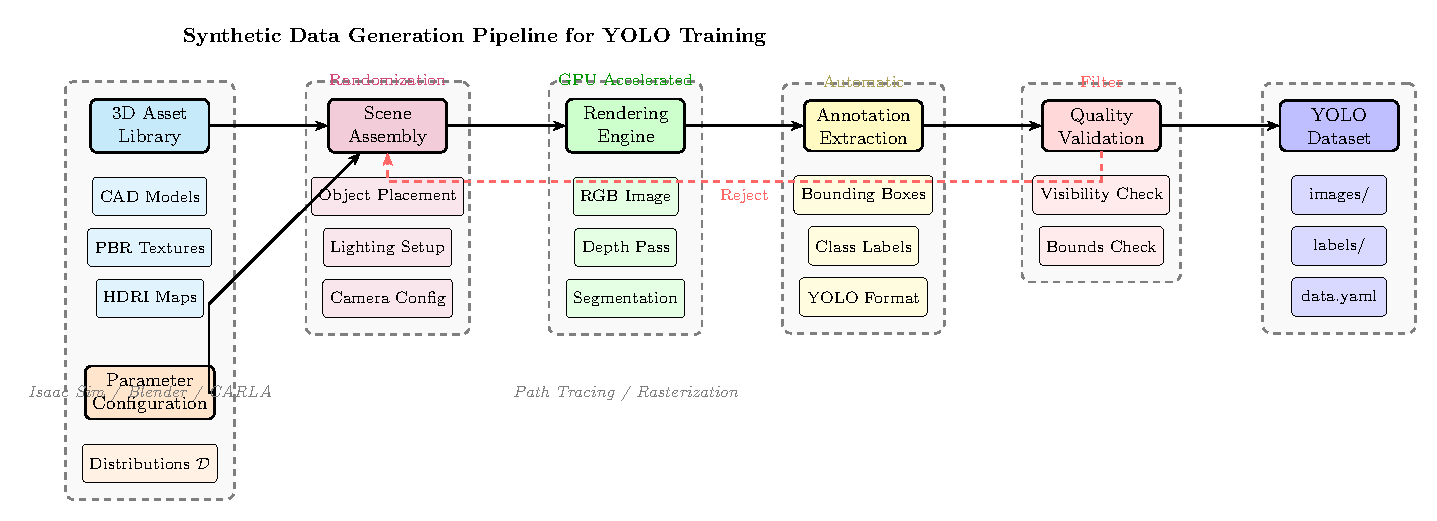
\includegraphics[width=\textwidth]{figures/ch04_fig1_sdg_pipeline.pdf}
\caption{End-to-end synthetic data generation pipeline for YOLO training. The pipeline encompasses six major stages: input preparation (3D assets and parameter configuration), scene assembly with domain randomization, GPU-accelerated rendering, automatic annotation extraction in YOLO format, quality validation with rejection loops, and final dataset output. Each stage is color-coded to indicate its primary function, with dashed arrows showing the rejection feedback loop for failed samples.}
\label{fig:sdg_pipeline}
\end{figure}

\section{Synthetic Data Generation Frameworks}
\label{sec:frameworks}

The landscape of synthetic data generation tools encompasses both general-purpose rendering engines and specialized simulation platforms designed specifically for machine learning applications. This section provides detailed descriptions of the major frameworks, their architectural approaches, and guidance for framework selection.

\subsection{NVIDIA Omniverse and Isaac Sim}

NVIDIA Isaac Sim represents the current state-of-the-art in synthetic data generation for robotics and computer vision applications. Built upon the NVIDIA Omniverse platform, Isaac Sim provides a comprehensive suite of tools for generating photorealistic imagery with precise ground truth annotations. The platform leverages NVIDIA's RTX technology for hardware-accelerated ray tracing, enabling the generation of physically accurate lighting, reflections, and shadows that closely approximate real-world optical phenomena.

The core synthetic data generation capability within Isaac Sim is provided through the Omniverse Replicator extension. This extension implements a domain-specific language for defining randomization distributions over scene parameters, enabling researchers to specify stochastic, controlled, and bounded parameter variations. The Replicator generates data in simulation rather than requiring real-world collection, automatically producing labels that can be directly consumed by training pipelines. This eliminates the preprocessing steps typically required when working with manually annotated datasets.

Isaac Sim's synthetic data generation capabilities span multiple approaches depending on the application requirements. Scene-based generation involves constructing complete 3D environments with semantically meaningful object placements, while object-based generation focuses on capturing individual objects from multiple viewpoints against varied backgrounds. Environment-based generation leverages procedurally generated worlds from tools like Infinigen to create diverse outdoor scenes. The platform also supports pose estimation synthetic data generation, implementing domain randomization techniques inspired by NVIDIA's research on the MESH and DOME datasets.

A distinguishing feature of Isaac Sim is its integration with SimReady assets, which are OpenUSD-based 3D models with built-in semantic labeling, dense captions, and physics properties based on USDPhysics. These assets streamline the simulation setup process by providing ready-to-use models with appropriate physical properties for realistic scene dynamics. The SimReady Warehouse 01 Assets Pack, for example, includes extensive collections of industrial objects such as pallets, storage racks, and ramps that are immediately usable for warehouse robotics applications.

Practical applications of Isaac Sim have demonstrated impressive results. One notable case study involved training a deep neural network to detect forklifts for collision avoidance with autonomous mobile robots, generating over 90,000 training images. Another application generated a synthetic dataset of 5,000 images for pallet jack detection in warehouse environments, applying domain randomization to pallet jack colors, poses, and camera positions while varying lighting and object placement.

\subsection{Blender with Python Scripting}

Blender represents a highly accessible and flexible option for synthetic data generation, combining professional-grade 3D rendering capabilities with extensive Python scripting support. As an open-source application licensed under the GNU General Public License, Blender eliminates licensing costs while providing rendering quality comparable to commercial alternatives. The Python API enables complete automation of scene construction, object manipulation, and batch rendering operations.

Blender offers two primary rendering engines with distinct performance and quality characteristics. The Cycles engine implements unbiased path tracing, simulating realistic light transport through the scene by tracing rays from the camera through multiple bounces until they reach light sources. This approach accurately captures global illumination effects including indirect lighting, color bleeding, and caustics. Research has demonstrated that path tracing consistently outperforms rasterization-based rendering across object detection benchmarks, with performance differences ranging from 0.3\% to 5.1\% mAP@50 depending on the specific use case. The Eevee engine provides real-time rasterization-based rendering that executes substantially faster but produces less physically accurate results.

\begin{figure}[htbp]
\centering
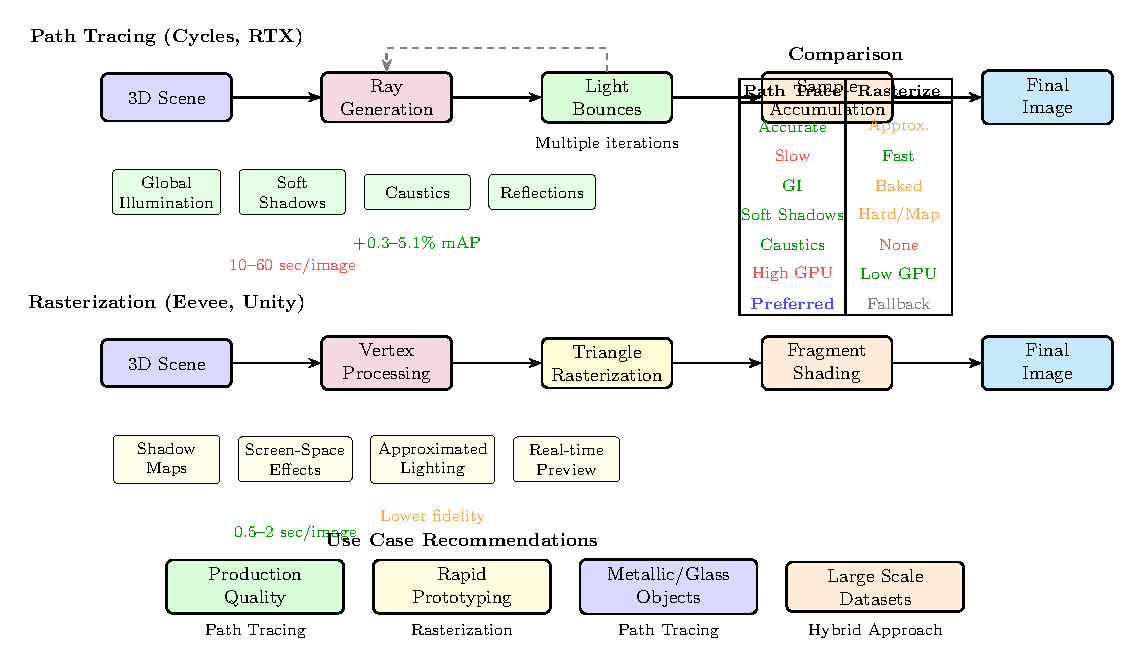
\includegraphics[width=\textwidth]{figures/ch04_fig3_rendering_comparison.pdf}
\caption{Comparison of path tracing and rasterization rendering pipelines for synthetic data generation. Path tracing (top) simulates realistic light transport through multiple bounces, producing physically accurate global illumination, soft shadows, and caustics at the cost of longer render times (10--60 seconds per image). Rasterization (bottom) uses projection and fragment shading for real-time preview speeds (0.5--2 seconds per image) with approximated lighting effects. The comparison table and use case recommendations guide practitioners in selecting the appropriate rendering approach for their application requirements.}
\label{fig:rendering_comparison}
\end{figure}

Several Python libraries extend Blender's capabilities specifically for synthetic data generation. The Starfish library, developed for spacecraft pose estimation, provides utilities for generating long sequences of synthetic images with intuitive parameter specifications. Starfish includes an annotation module with utility functions for generating segmentation masks using Blender's ID Mask Node system. Other notable libraries include BlenderProc, which implements a modular pipeline for synthetic data generation with support for common annotation formats.

A typical Blender-based synthetic data pipeline involves programmatically loading 3D object models, randomizing their positions, rotations, and scales, configuring lighting and camera parameters, rendering the scene to an image file, and extracting ground truth annotations from the scene graph. The bpy module provides access to all Blender functionality from Python, enabling scripts to modify virtually any aspect of the scene. Ground truth extraction leverages Blender's ability to render object indices into auxiliary passes, which can then be processed to generate bounding boxes, segmentation masks, or keypoint annotations.

\subsection{Infinigen Procedural Generation}

Infinigen represents a paradigm shift in synthetic data generation through its entirely procedural approach. Developed by the Princeton Vision and Learning Lab and presented at CVPR 2023, Infinigen generates all scene content from randomized mathematical rules without relying on any external assets or scanned geometry. This procedural foundation enables infinite variation at both the object and scene levels, as each generation produces genuinely novel content rather than sampling from a fixed asset library.

The system covers a broad range of natural world content including procedurally generated plants, animals, terrains, and natural phenomena such as fire, clouds, rain, and snow. Each category of content is defined by mathematical functions that capture the essential characteristics of the object class while admitting substantial variation through parameter randomization. A procedurally generated tree, for example, follows botanical growth rules that produce realistic branching structures, bark textures, and leaf distributions, yet each generated instance is unique.

Infinigen Indoors, presented at CVPR 2024, extends the system to indoor environments by introducing procedural generators for furniture, architectural elements, appliances, and everyday objects. The indoor extension also introduces a constraint-based arrangement system with a domain-specific language for expressing diverse constraints on scene composition. This enables the generation of semantically coherent room layouts where objects are placed according to functional relationships rather than purely random positioning.

The ground truth outputs from Infinigen are comprehensive, including RGB imagery, metric depth maps, surface normals, occlusion boundaries, pixel-level semantic and instance segmentation, 3D bounding boxes, optical flow, and per-object semantic labels. These outputs are exported in standard formats including PNG, EXR, JSON, and NPZ for direct consumption by training pipelines. For embodied agent training, Infinigen provides export to URDF, USD, and MJCF formats that can be directly loaded into real-time simulators such as Omniverse, Unreal Engine, and MuJoCo.

\subsection{Unity Perception}

Unity Perception was developed by Unity Technologies as a toolkit for generating synthetic datasets for perception-based machine learning tasks. The package provided tools for object detection, semantic segmentation, pose estimation, and related computer vision applications. The system was integrated into the Unity game engine, leveraging Unity's mature 3D rendering pipeline and extensive asset ecosystem.

The Perception package architecture centered on the Perception Camera component, which captured synthetic sensor data from simulated cameras within the Unity scene. Camera Labelers attached to the Perception Camera specified which types of ground truth to generate, such as 2D bounding boxes, semantic segmentation masks, or 3D keypoints. The Randomizer system implemented domain randomization by modifying scene parameters between captured frames according to specified probability distributions.

The SynthDet project demonstrated an end-to-end object detection pipeline using Unity Perception, generating highly randomized images of 63 common grocery products with 2D bounding box annotations. This project showcased the potential for training performant object detection models entirely on synthetic data generated within the Unity environment.

It should be noted that the Unity Perception project has been discontinued and is no longer officially supported by Unity Technologies. The repository remains available for reference and community support, but developers should consider alternative frameworks for new projects requiring long-term maintenance and support.

\subsection{CARLA for Autonomous Driving}

CARLA represents a domain-specific simulator purpose-built for autonomous driving research. Unlike general-purpose rendering engines, CARLA provides a complete simulation environment including urban and rural road networks, traffic simulation, pedestrian behavior models, and realistic vehicle dynamics. This domain specificity enables the generation of training data that captures the contextual regularities present in real driving scenarios.

The CARLA sensor suite is among the most comprehensive available for driving simulation, supporting RGB cameras, depth cameras, semantic segmentation cameras, instance segmentation, LIDAR sensors, and radar sensors. Each sensor type accurately simulates critical parameters including field of view, resolution, range accuracy, and scanning frequency. The multi-sensor configuration enables generation of datasets with complementary modalities for sensor fusion research.

Weather simulation in CARLA encompasses sun position (time of day), cloud cover, precipitation intensity and type, fog density, and wind effects on vegetation. Research has demonstrated that models trained on CARLA images without domain randomization achieved only one-third of the average precision compared to models with weather and lighting variation enabled. This finding underscores the importance of environmental diversity in synthetic training data.

Several tools have been developed to facilitate dataset generation from CARLA. The CarFree tool automates diverse driving scenario generation under varied weather and lighting conditions, extracting ground truth through post-processing of RGB images, semantic segmentation, and 3D object locations. CARLA-KITTI provides scripts for generating synthetic data in the KITTI benchmark format for direct comparison with real-world driving datasets. CARLA2Real applies photorealism enhancement through neural style transfer to reduce the visual domain gap between synthetic and real imagery.

\subsection{Framework Comparison}

Table~\ref{tab:framework_comparison} provides a systematic comparison of the major synthetic data generation frameworks across dimensions relevant to object detection training.

\begin{table}[htbp]
\centering
\caption{Comparison of Synthetic Data Generation Frameworks}
\label{tab:framework_comparison}
\begin{tabular}{p{2.5cm}p{2cm}p{2cm}p{2cm}p{2cm}p{2cm}}
\hline
\textbf{Feature} & \textbf{Isaac Sim} & \textbf{Blender} & \textbf{Infinigen} & \textbf{Unity} & \textbf{CARLA} \\
\hline
Rendering Quality & Excellent & Excellent & Excellent & Good & Good \\
Path Tracing & Yes & Yes (Cycles) & Yes & Limited & No \\
Python API & Yes & Yes & Yes & C\# Primary & Yes \\
PBR Materials & Yes & Yes & Yes & Yes & Limited \\
Physics Simulation & Yes & Yes & Yes & Yes & Yes \\
Domain Randomization & Built-in & Scripted & Procedural & Built-in & Scripted \\
YOLO Export & Direct & Scripted & JSON/NPZ & SOLO Format & KITTI \\
License & Proprietary & GPL & BSD 3-Clause & Proprietary & MIT \\
GPU Requirements & High (RTX) & Moderate & Moderate & Moderate & High \\
Learning Curve & Moderate & Moderate & Low & Moderate & Low \\
Active Development & Yes & Yes & Yes & Discontinued & Yes \\
Best Use Case & Robotics & Flexible & Environments & Legacy & Driving \\
\hline
\end{tabular}
\end{table}

The selection of an appropriate framework depends on the specific application requirements, computational resources, and team expertise. Isaac Sim is recommended for production robotics applications requiring the highest fidelity synthetic data and integration with NVIDIA's broader AI toolchain. Blender with Python scripting provides maximum flexibility for custom pipelines and is recommended for research applications and teams with existing Blender expertise. Infinigen excels at generating diverse environmental content and is recommended when maximum scene variation is required. CARLA remains the standard for autonomous driving research due to its domain-specific simulation capabilities.

\begin{figure}[htbp]
\centering
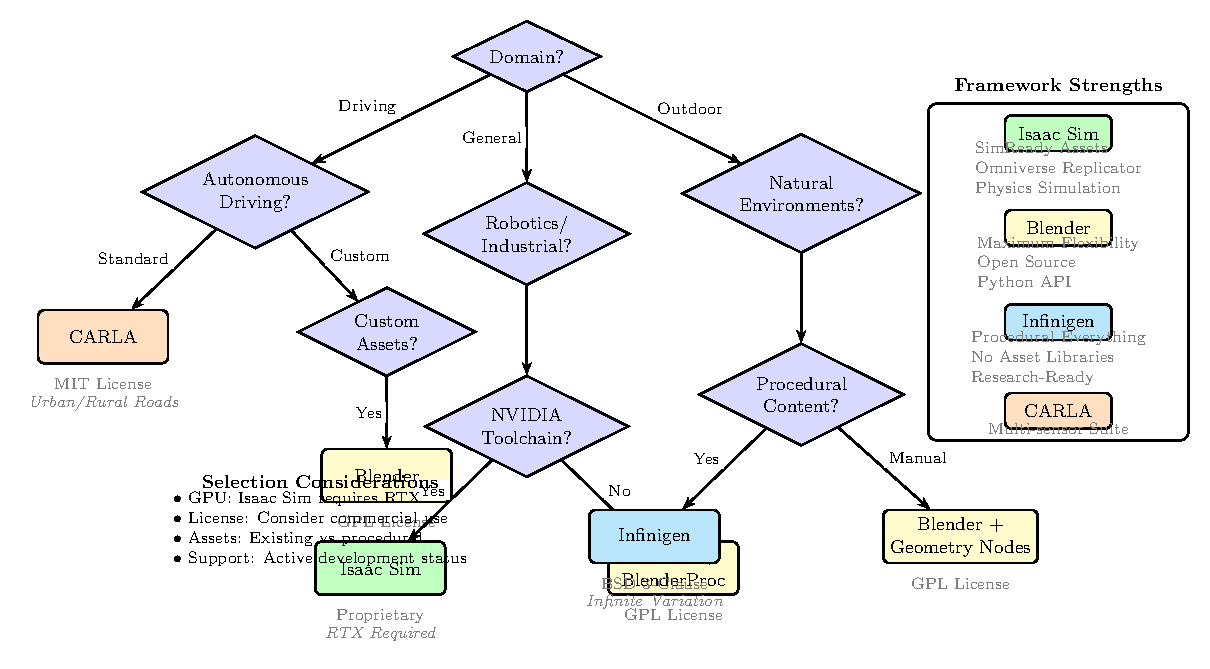
\includegraphics[width=\textwidth]{figures/ch04_fig4_framework_selection.pdf}
\caption{Decision tree for synthetic data generation framework selection. The tree guides practitioners through key decision points including application domain (driving, robotics, natural environments), integration requirements (NVIDIA toolchain compatibility), and content generation approach (procedural vs. asset-based). Framework strengths and licensing considerations are summarized in the accompanying reference panels.}
\label{fig:framework_selection}
\end{figure}

\section{Complete Parameter Taxonomy}
\label{sec:parameter_taxonomy}

This section presents an exhaustive taxonomy of tunable parameters for synthetic data generation, organized by functional category. For each parameter, we provide descriptions, typical ranges observed in the literature, and implementation considerations.

\begin{figure}[htbp]
\centering
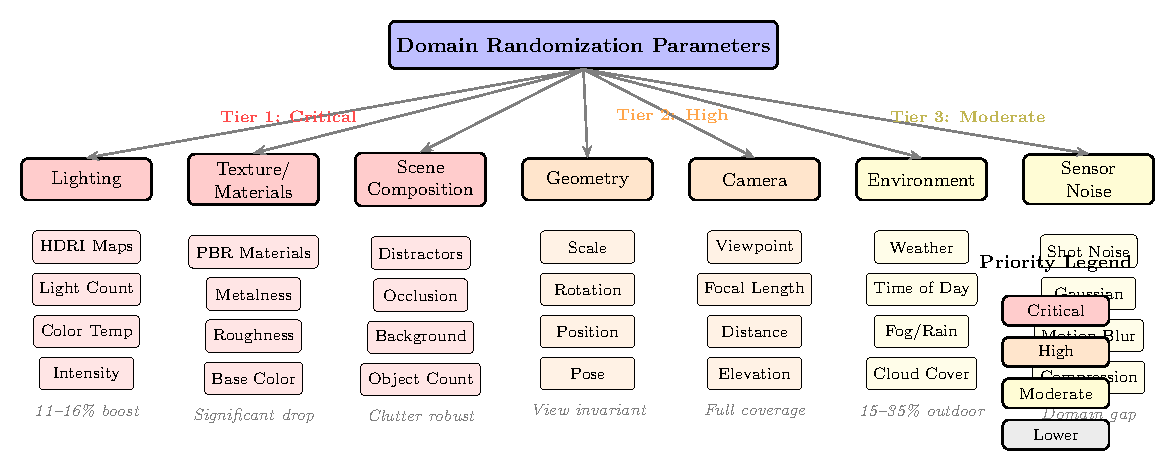
\includegraphics[width=\textwidth]{figures/ch04_fig2_parameter_taxonomy.pdf}
\caption{Hierarchical taxonomy of domain randomization parameters organized by priority tier. Tier 1 (Critical) parameters---lighting, texture/materials, and scene composition---demonstrate the largest impact on real-world detection performance. Tier 2 (High) parameters include geometry and camera settings. Tier 3 (Moderate) parameters cover environmental effects and sensor noise. Evidence-based impact annotations are shown below each parameter category.}
\label{fig:parameter_taxonomy}
\end{figure}

\subsection{Object Appearance Parameters}

Object appearance encompasses the visual properties of target objects and scene elements that determine their rendered appearance. These parameters directly influence the features that neural networks extract during training and are among the most critical for achieving robust real-world generalization.

\subsubsection{Texture Types}

Textures define the surface appearance of 3D objects and are typically implemented through one of three approaches. RGB textures assign uniform or randomly sampled color values to object surfaces, providing basic appearance variation with minimal computational overhead. This approach is commonly used in aggressive domain randomization where photorealism is sacrificed for maximum variation. Image-based textures apply photographic images to object surfaces through UV mapping, providing realistic surface detail at the cost of requiring texture asset libraries. Physically Based Rendering (PBR) textures represent the current state of the art, defining surface appearance through physically meaningful parameters including base color, metalness, roughness, and normal maps. Research has demonstrated that PBR materials produce superior results for reflective and metallic objects, with ablation studies showing significant performance drops when random textures are substituted for PBR materials.

\subsubsection{Material Properties}

Beyond texture mapping, material properties define how surfaces interact with light. Metalness, ranging from 0 (dielectric) to 1 (fully metallic), determines whether the surface exhibits diffuse reflection or metallic specular behavior. Roughness, also ranging from 0 to 1, controls the sharpness of specular reflections, with low values producing mirror-like reflections and high values producing diffuse highlights. Subsurface scattering simulates light penetration into translucent materials such as skin, wax, or vegetation. Index of refraction, typically ranging from 1.0 to 2.5, affects the intensity of specular reflections at grazing angles according to Fresnel equations.

\subsubsection{Color Variation Strategies}

Color variation may be implemented through several complementary strategies. Hue shifting rotates all colors in the image by a specified angular offset, typically limited to $\pm20$ degrees to maintain plausible appearances. Saturation adjustment scales color intensity between 0 (grayscale) and 150\% of original values. Value or brightness adjustment modifies overall luminance by $\pm30\%$. For object-specific variation, base colors may be sampled from predefined palettes that match the expected real-world color distributions for each object class.

Table~\ref{tab:appearance_params} summarizes the object appearance parameters with their typical ranges.

\begin{table}[htbp]
\centering
\caption{Object Appearance Parameters}
\label{tab:appearance_params}
\begin{tabular}{p{3.5cm}p{3cm}p{5cm}}
\hline
\textbf{Parameter} & \textbf{Typical Range} & \textbf{Implementation Notes} \\
\hline
Texture Type & RGB, Image, PBR & PBR preferred for reflective objects \\
Base Color & RGB [0,255] per channel & Sample from realistic color distributions \\
Metalness & [0.0, 1.0] & 0 for plastics, 1 for metals \\
Roughness & [0.0, 1.0] & 0.3--0.8 covers most real materials \\
Subsurface & [0.0, 1.0] & Enable for translucent materials \\
Index of Refraction & [1.0, 2.5] & 1.5 typical for glass and plastic \\
Normal Map Strength & [0.0, 2.0] & 1.0 is physically correct \\
Hue Shift & $[-20, +20]$ degrees & Larger shifts may appear unrealistic \\
Saturation Scale & [0.5, 1.5] & Maintain within plausible range \\
\hline
\end{tabular}
\end{table}

\subsection{Geometric Variation Parameters}

Geometric parameters control the spatial properties of objects including their size, orientation, and position. Adequate geometric variation is essential for training detectors that generalize across the range of object appearances expected in deployment.

\subsubsection{Scale Variations}

Scale variation simulates objects at different distances from the camera and natural variation in object size. Uniform scaling applies identical scale factors to all axes, typically ranging from 0.5$\times$ to 2.0$\times$ baseline size. Non-uniform scaling applies different factors per axis to simulate aspect ratio variation, typically constrained to 0.8$\times$ to 1.2$\times$ per axis to maintain object recognizability. Scale distributions should match the expected real-world size distribution, which may be obtained from domain knowledge or small real-world samples.

\subsubsection{Rotation Variations}

Rotation may be specified in Euler angles or quaternion representation. Full rotation covers all orientations with uniform sampling over SO(3), which is appropriate for objects without a natural upright orientation. Constrained rotation limits rotation to specified angular ranges, such as $\pm30$ degrees from upright, for objects that are typically observed in canonical orientations. Research has shown that appropriately constraining rotation based on domain knowledge improves detection performance compared to unrestricted rotation.

\subsubsection{Translation and Placement}

Object translation determines spatial position within the scene. Random placement samples positions uniformly within scene bounds but may produce unrealistic floating objects or interpenetrations. Physics-based placement enables objects to fall under gravity and settle on surfaces, producing realistic resting positions. Semantic placement positions objects according to functional relationships, such as dishes on tables or products on shelves.

\subsubsection{Pose Variation for Articulated Objects}

For articulated objects such as human figures, robotic arms, or animals, pose variation involves randomizing joint angles within their valid ranges. Each joint is typically parameterized by one to three rotation degrees of freedom with associated minimum and maximum angle limits. Pose sampling may be uniform within joint limits or weighted toward commonly observed configurations.

Table~\ref{tab:geometric_params} presents the complete geometric variation parameter set.

\begin{table}[htbp]
\centering
\caption{Geometric Variation Parameters}
\label{tab:geometric_params}
\begin{tabular}{p{3.5cm}p{3cm}p{5cm}}
\hline
\textbf{Parameter} & \textbf{Typical Range} & \textbf{Implementation Notes} \\
\hline
Uniform Scale & [0.5, 2.0] & Match expected distance variation \\
Per-Axis Scale & [0.8, 1.2] & Subtle aspect ratio variation \\
Rotation (Full) & [0, 360] all axes & Uniform sampling over SO(3) \\
Rotation (Constrained) & $\pm$30 degrees & Apply domain-appropriate limits \\
Translation X, Y & Scene bounds & Ensure object remains visible \\
Translation Z (Height) & [0, scene height] & Physics placement preferred \\
Joint Angles & Joint-specific limits & Valid kinematic configurations \\
\hline
\end{tabular}
\end{table}

\subsection{Scene Composition Parameters}

Scene composition determines the spatial arrangement of objects within the rendered environment, including object counts, occlusion relationships, and background content. These parameters have substantial impact on model robustness to cluttered real-world scenes.

\subsubsection{Object Density and Placement Strategies}

Object density specifies the number of target objects per rendered scene. Low density configurations with 1--3 objects simplify detection but may not prepare models for crowded scenarios. High density configurations with 10--20+ objects improve robustness to crowding but require careful management of occlusion levels. Placement strategies include uniform random sampling within scene bounds, grid-based placement with jittered positions, and constraint-based placement that respects spatial relationships.

\subsubsection{Occlusion Level Control}

Occlusion presents one of the most challenging aspects of real-world object detection, and synthetic data generation provides precise control over occlusion levels. Occlusion may be quantified as the percentage of object pixels visible (100\% minus occlusion percentage). Research categorizes occlusion into levels: no occlusion (100\% visibility), light occlusion (75--100\% visibility), moderate occlusion (50--75\% visibility), and heavy occlusion (25--50\% visibility). Training data should include examples across all occlusion levels with empirically determined distributions such as 40\% no occlusion, 30\% light, 20\% moderate, and 10\% heavy.

\subsubsection{Distractor Objects}

Distractor objects are non-target objects placed in scenes to increase visual complexity and train models to reject false positive detections. Research has demonstrated that including large numbers of distractor models, with studies using up to 15,000 unique distractors, improves detection robustness in cluttered environments. Distractors may be randomly selected from object databases such as Objaverse or domain-specific collections. The number of distractors per scene typically ranges from 0 to 50 depending on target scene complexity.

\subsubsection{Background Generation}

Background generation strategies significantly impact domain transfer. Random image backgrounds sample from large photographic databases such as ImageNet or Flickr to provide maximum appearance variation. Rendered 3D environments provide physically consistent backgrounds with proper lighting interaction. HDRI environment maps provide realistic 360-degree backgrounds captured from real locations. Research indicates that real photograph backgrounds composited behind rendered foreground objects improve sim-to-real transfer compared to purely synthetic backgrounds.

Table~\ref{tab:composition_params} summarizes scene composition parameters.

\begin{table}[htbp]
\centering
\caption{Scene Composition Parameters}
\label{tab:composition_params}
\begin{tabular}{p{3.5cm}p{3cm}p{5cm}}
\hline
\textbf{Parameter} & \textbf{Typical Range} & \textbf{Implementation Notes} \\
\hline
Target Object Count & [1, 20+] & Match expected scene density \\
Distractor Count & [0, 50] & Higher values for cluttered scenes \\
Occlusion Level & [0\%, 90\%] & Include distribution across levels \\
Placement Strategy & Random, Physics, Semantic & Physics-based most realistic \\
Background Type & Image, 3D, HDRI & Real photographs improve transfer \\
Scene Clutter Level & Low, Medium, High & Varies distractor density \\
Minimum Object Visibility & [10\%, 50\%] & Filter heavily occluded instances \\
\hline
\end{tabular}
\end{table}

\subsection{Lighting Parameters}

Lighting parameters control the illumination of synthetic scenes and represent one of the most impactful categories for detection performance. Research has consistently demonstrated that lighting variation during training substantially improves real-world generalization.

\subsubsection{Light Count and Configuration}

The number of light sources significantly affects scene appearance and shadow complexity. Single-light configurations produce hard, directional shadows while multi-light setups with 3--12 lights create more complex, realistic illumination. Point lights emit in all directions from a position in space. Area lights emit from a surface and produce soft shadows proportional to the light size. Directional lights simulate distant sources like the sun. Spot lights emit in a cone and are used for focused illumination.

\subsubsection{Light Position and Orientation}

Light positioning is typically specified in spherical coordinates relative to the scene center. Azimuth angle, ranging from 0 to 360 degrees, determines the horizontal direction. Elevation angle, ranging from 0 (horizon) to 90 (directly above), determines height. Distance affects intensity falloff. Full coverage of the hemisphere ensures the model sees objects illuminated from all directions.

\subsubsection{Intensity and Falloff}

Light intensity is specified in physically-based units such as watts or lumens, or in relative terms as a multiplier on baseline illumination. Intensity variation typically spans a 10$\times$ range on a logarithmic scale to cover dim indoor to bright outdoor conditions. Falloff follows inverse square law for physically accurate distance attenuation, though linear or constant falloff may be used for artistic control.

\subsubsection{Color Temperature}

Color temperature, measured in Kelvin, determines the spectral distribution of emitted light. Warm lighting at 2700--3500K matches incandescent sources and produces orange-yellow illumination. Neutral lighting at 4000--5000K matches daylight fluorescents. Cool lighting at 5500--6500K matches overcast daylight. Extended range up to 10000K covers blue sky illumination. Randomizing color temperature exposes models to the range of real-world illumination conditions.

\subsubsection{HDRI Environment Maps}

High Dynamic Range Image (HDRI) environment maps capture real-world lighting environments as 360-degree panoramic images with extended dynamic range. Each pixel stores both color and intensity for a specific direction, enabling physically accurate image-based lighting. Research has demonstrated that HDRI lighting produces an 11.11\% boost in classification accuracy and 16.04\% increase in AUC compared to simple directional lighting. HDRI databases such as Poly Haven provide hundreds of free environment maps covering indoor, outdoor, studio, and industrial settings.

\subsubsection{Shadow Characteristics}

Shadow appearance depends on light type and size. Point lights produce sharp shadows with hard edges. Area lights produce soft shadows with penumbra regions proportional to light size relative to occluder distance. Shadow density may be controlled by adjusting light intensities. Multiple lights create complex overlapping shadow patterns. Including shadow variation during training improves robustness to real-world lighting.

Table~\ref{tab:lighting_params} presents the complete lighting parameter set.

\begin{table}[htbp]
\centering
\caption{Lighting Parameters}
\label{tab:lighting_params}
\begin{tabular}{p{3.5cm}p{3cm}p{5cm}}
\hline
\textbf{Parameter} & \textbf{Typical Range} & \textbf{Implementation Notes} \\
\hline
Light Count & [1, 12] & Higher counts for complex illumination \\
Light Type & Point, Area, Directional & Mix types for realism \\
Position Azimuth & [0, 360] degrees & Full horizontal coverage \\
Position Elevation & [0, 90] degrees & Above-horizon positions \\
Intensity & [0.1, 10.0]$\times$ baseline & Log-scale sampling \\
Color Temperature & [2700, 10000] K & Match expected conditions \\
Area Light Size & [0.1, 2.0] meters & Affects shadow softness \\
Ambient Intensity & [0, 100]\% of total & Fills shadow regions \\
HDRI Environment & Database index & Randomize across collection \\
\hline
\end{tabular}
\end{table}

\subsection{Camera Parameters}

Camera parameters define the simulated imaging system, including optical properties and sensor configuration. Matching these parameters to the deployment camera improves domain transfer.

\subsubsection{Focal Length and Field of View}

Focal length, typically specified in 35mm equivalent millimeters, determines the field of view and perspective distortion characteristics. Wide-angle lenses with 18--35mm focal length capture more scene content but introduce perspective distortion. Normal lenses with 35--70mm approximate human vision. Telephoto lenses with 70--200mm compress perspective and narrow field of view. Field of view may alternatively be specified directly, typically ranging from 30 to 120 degrees.

\subsubsection{Lens Distortion Models}

Real camera lenses introduce geometric distortion that must be modeled for accurate synthetic data. Barrel distortion causes straight lines to curve outward from the image center. Pincushion distortion causes lines to curve inward. The Brown-Conrady model parameterizes distortion using radial coefficients $k_1$, $k_2$, $k_3$ and tangential coefficients $p_1$, $p_2$. Distortion parameters should be calibrated from the target deployment camera for maximum fidelity.

\subsubsection{Motion Blur Simulation}

Motion blur occurs when objects move relative to the camera during exposure. Object motion blur affects moving objects within the scene. Camera motion blur affects the entire image when the camera platform moves. Motion blur is typically specified by exposure time, with 0--50ms exposure producing varying degrees of blur depending on motion velocity. Motion blur should be included when training for detection of moving objects or from mobile platforms.

\subsubsection{Depth of Field}

Depth of field effects blur objects outside the focal plane. Aperture setting controls blur intensity, with wide apertures (low f-numbers like f/1.4) producing shallow depth of field and narrow apertures (high f-numbers like f/22) producing deep focus. For object detection, depth of field effects are typically disabled or minimized as they can obscure relevant image features. However, including moderate depth of field variation may improve robustness when deploying to cameras with limited hyperfocal capabilities.

Table~\ref{tab:camera_params} details camera parameters.

\begin{table}[htbp]
\centering
\caption{Camera Parameters}
\label{tab:camera_params}
\begin{tabular}{p{3.5cm}p{3cm}p{5cm}}
\hline
\textbf{Parameter} & \textbf{Typical Range} & \textbf{Implementation Notes} \\
\hline
Focal Length & [18, 200] mm & Match deployment camera \\
Field of View & [30, 120] degrees & Alternative to focal length \\
Camera Distance & [0.5, 5.0] meters & Determines object scale \\
Camera Azimuth & [0, 360] degrees & Full horizontal coverage \\
Camera Elevation & [-30, 90] degrees & Above and below horizon \\
Camera Roll & [-15, 15] degrees & Slight tilts only \\
Distortion $k_1$ & [-0.5, 0.5] & Calibrate from real camera \\
Distortion $k_2$ & [-0.2, 0.2] & Higher-order correction \\
Motion Blur & [0, 50] ms exposure & For dynamic scenarios \\
Aperture & f/1.4 to f/22 & Controls depth of field \\
\hline
\end{tabular}
\end{table}

\subsection{Environmental Parameters}

Environmental parameters simulate atmospheric and weather conditions that affect outdoor imagery. These parameters are essential for applications deployed in variable weather conditions.

\subsubsection{Weather Effects}

Rain simulation involves rendering falling droplets, wet surface reflections, and reduced visibility. Physics-based rain rendering adds realistic rain streaks and splashing effects. Research has demonstrated 15\% improvement in object detection and 35\% improvement in semantic segmentation when training includes rain-augmented data. Fog simulation reduces visibility through exponential or exponential-squared falloff with distance. Visibility distances typically range from 100m (dense fog) to 10km (light haze). Snow simulation combines falling particles with ground accumulation and reduced visibility.

\subsubsection{Time of Day Simulation}

Time of day determines sun position and color, sky appearance, and overall scene illumination. Solar position is calculated from geographic location and time. Dawn and dusk produce warm, directional illumination with long shadows. Midday produces harsh overhead illumination. Night requires artificial lighting sources. Sky color transitions from warm oranges at horizon to deep blues at zenith during golden hour.

Table~\ref{tab:environmental_params} presents environmental parameters.

\begin{table}[htbp]
\centering
\caption{Environmental Parameters}
\label{tab:environmental_params}
\begin{tabular}{p{3.5cm}p{3cm}p{5cm}}
\hline
\textbf{Parameter} & \textbf{Typical Range} & \textbf{Implementation Notes} \\
\hline
Time of Day & [0, 24] hours & Affects sun position and color \\
Cloud Cover & [0, 100]\% & Affects diffuse lighting \\
Rain Intensity & [0, 100] mm/hr & Include streaks and puddles \\
Fog Visibility & [100, 10000] meters & Exponential falloff model \\
Snow Intensity & Light, Medium, Heavy & Combine with fog \\
Wet Surface & Dry, Wet, Puddled & Increases specularity \\
Wind Speed & [0, 30] m/s & Affects vegetation motion \\
\hline
\end{tabular}
\end{table}

\subsection{Sensor Noise Parameters}

Sensor noise parameters simulate the imperfections inherent in real camera systems. Appropriate noise modeling is critical for bridging the domain gap between synthetic and real imagery.

\subsubsection{Gaussian Noise}

Additive white Gaussian noise (AWGN) represents random intensity variations independent of signal level. Gaussian noise is characterized by its standard deviation $\sigma$, typically ranging from 0 to 25 on an 8-bit [0, 255] scale. While AWGN is commonly used for its simplicity, it does not accurately represent real camera noise, which is signal-dependent.

\subsubsection{Shot Noise}

Shot noise, also called photon noise, arises from the discrete nature of photon arrivals at the sensor. Shot noise follows a Poisson distribution where variance equals the mean signal level, causing brighter regions to exhibit more noise than darker regions. Physics-based shot noise simulation improves realism compared to uniform Gaussian noise.

\subsubsection{Salt-and-Pepper Noise}

Salt-and-pepper noise simulates sensor defects that cause pixels to read at maximum (white) or minimum (black) values. The noise is characterized by the probability of pixel corruption, typically ranging from 0 to 5\%. This noise type simulates dead pixels and transmission errors.

\subsubsection{ISO Simulation}

ISO setting on real cameras controls sensor sensitivity by adjusting analog and digital gain. Higher ISO values amplify both signal and noise, increasing image brightness at the cost of increased noise visibility. ISO simulation typically ranges from 100 (low noise) to 12800 (high noise), with noise characteristics varying based on the simulated sensor model.

\subsubsection{Compression Artifacts}

JPEG and video compression introduce blocking artifacts, ringing around edges, and color quantization. Compression quality settings from 50\% (heavy compression) to 100\% (minimal compression) control artifact severity. Including compression artifacts in training data improves robustness when deploying to systems with compressed video pipelines.

Table~\ref{tab:noise_params} summarizes sensor noise parameters.

\begin{table}[htbp]
\centering
\caption{Sensor Noise Parameters}
\label{tab:noise_params}
\begin{tabular}{p{3.5cm}p{3cm}p{5cm}}
\hline
\textbf{Parameter} & \textbf{Typical Range} & \textbf{Implementation Notes} \\
\hline
Gaussian $\sigma$ & [0, 25] 8-bit scale & Simple but not realistic \\
Shot Noise & Signal-dependent & Poisson model preferred \\
Salt-and-Pepper & [0, 5]\% pixels & Simulate sensor defects \\
Read Noise & Camera-specific & From sensor datasheet \\
Dark Current & Temperature-dependent & Low priority \\
ISO Equivalent & [100, 12800] & Higher = more noise \\
JPEG Quality & [50, 100]\% & For compressed pipelines \\
\hline
\end{tabular}
\end{table}

\section{Parameter Priority Ranking}
\label{sec:priority_ranking}

This section presents an evidence-based ranking of parameter importance derived from ablation studies and empirical research in the synthetic data generation literature. Understanding parameter priority enables efficient allocation of effort and computational resources during synthetic dataset construction.

\subsection{Tier 1: Critical Impact Parameters}

Tier 1 parameters have demonstrated the largest impact on real-world detection performance in controlled experiments. These parameters should receive priority attention in any synthetic data generation pipeline.

Dataset diversity and scale represents the most impactful factor overall. Research on YOLOv11 demonstrated that expanding the dataset with varied viewpoints and negative examples outperformed augmentation techniques applied to a smaller base dataset. The inclusion of images without target objects (negative examples) proved essential for reducing false positive rates in deployment.

Lighting variation consistently ranks among the most critical parameters. HDRI environment lighting produced 11.11\% improvement in classification accuracy compared to simple directional lighting. Multi-light configurations with randomized positions, intensities, and color temperatures ensure exposure to the range of illumination conditions encountered in real environments.

Object texture and material properties demonstrate substantial impact, particularly for reflective or metallic objects. Ablation studies found that excluding random textures or reducing texture variants resulted in significant performance drops. PBR materials that accurately model surface reflectance outperform simple RGB color assignments.

Background and scene composition directly impacts the model's ability to distinguish target objects from visual clutter. Real photograph backgrounds improve domain transfer compared to purely synthetic backgrounds. Including diverse distractor objects, with research using up to 15,000 unique distractor models, trains models to reject false positive detections.

Camera viewpoint variation ensures the model observes objects from all angles. Full azimuth coverage (0--360 degrees) and broad elevation coverage (-30 to +90 degrees) are necessary for viewpoint-invariant detection.

\subsection{Tier 2: High Impact Parameters}

Tier 2 parameters have demonstrated meaningful impact on detection performance and should be included when computational resources permit.

Occlusion level variation trains models to detect partially visible objects. Including examples across occlusion levels from 0\% to 75\% improves robustness to real-world scenarios where objects are frequently partially hidden.

Object scale variation prepares models for objects at different distances. Wide scale ranges (0.5$\times$ to 2.0$\times$ baseline) are necessary to match the range of apparent object sizes in deployment.

Rendering quality, specifically the choice between path tracing and rasterization, produces measurable differences. Path tracing consistently outperforms rasterization by 0.3\% to 5.1\% mAP@50, justifying the additional rendering time for critical applications.

Post-processing noise and blur, when appropriately calibrated, improve domain transfer. Ablation studies found that removing noise and blur effects caused performance drops, particularly in robotics and industrial applications.

Object rotation and pose variation ensures the model recognizes objects across their range of possible orientations. Constraints should be applied based on domain knowledge of expected object configurations.

\subsection{Tier 3: Moderate Impact Parameters}

Tier 3 parameters provide incremental improvements and should be included when sufficient resources are available.

Weather effects including rain, fog, and snow are essential for outdoor applications but may be omitted for controlled indoor environments. Research demonstrated 15--35\% improvement on weather-degraded test images when weather augmentation was included during training.

Color and brightness jitter through standard image augmentation provides moderate improvement with minimal computational cost. These augmentations are typically applied during training data loading rather than during rendering.

Distractor object diversity beyond baseline levels provides diminishing returns. While some distractor objects are essential (Tier 1), maximizing distractor variety provides incremental benefit.

Compositional augmentation techniques such as Mixup and Mosaic, applied during training, improve performance on cluttered scenes. These techniques combine multiple training images to create synthetic crowded scenarios.

\subsection{Tier 4: Lower Priority Parameters}

Tier 4 parameters provide minimal impact in most scenarios and may be omitted to reduce pipeline complexity.

Lens distortion modeling is necessary only when the deployment camera exhibits significant geometric distortion. For well-corrected lenses, distortion simulation provides minimal benefit.

Motion blur is relevant only for applications involving moving cameras or fast-moving objects. For static scene detection, motion blur may actually degrade performance.

Chromatic aberration produces subtle color fringing that is rarely visible in typical imaging conditions. The impact on detection performance is minimal.

Compression artifacts should be included when training for compressed video pipelines but may be omitted for uncompressed image detection.

Depth of field effects are generally not beneficial for detection tasks, as blur obscures object features. This effect should be minimized or disabled.

Table~\ref{tab:priority_ranking} summarizes the parameter priority ranking with supporting evidence.

\begin{table}[htbp]
\centering
\caption{Parameter Priority Ranking with Evidence}
\label{tab:priority_ranking}
\begin{tabular}{p{1cm}p{3.5cm}p{6cm}}
\hline
\textbf{Tier} & \textbf{Parameter Category} & \textbf{Evidence Summary} \\
\hline
1 & Dataset Diversity & Expanded datasets with negatives outperform augmentation \\
1 & Lighting Variation & HDRI: 11--16\% improvement over simple lighting \\
1 & Texture/Materials & Excluding textures causes significant performance drop \\
1 & Scene Composition & Distractors essential for clutter robustness \\
1 & Camera Viewpoint & Full coverage necessary for invariance \\
\hline
2 & Occlusion Levels & Trains for partially visible object detection \\
2 & Object Scale & Addresses distance variation \\
2 & Path Tracing & 0.3--5.1\% mAP improvement over rasterization \\
2 & Noise/Blur & Removing causes performance drops \\
2 & Rotation/Pose & Enables orientation invariance \\
\hline
3 & Weather Effects & 15--35\% improvement on degraded images \\
3 & Color Jitter & Standard augmentation, moderate impact \\
3 & Distractor Diversity & Diminishing returns beyond baseline \\
3 & Mixup/Mosaic & Helps with cluttered scenes \\
\hline
4 & Lens Distortion & Only for distorted deployment cameras \\
4 & Motion Blur & Only for dynamic scenarios \\
4 & Chromatic Aberration & Minimal visible impact \\
4 & Compression Artifacts & Only for compressed pipelines \\
4 & Depth of Field & Generally not beneficial \\
\hline
\end{tabular}
\end{table}

\section{Generation Pipeline Architecture}
\label{sec:pipeline_architecture}

This section describes the end-to-end architecture for synthetic data generation pipelines, including annotation format generation for YOLO training and quality control measures.

\subsection{End-to-End Pipeline Design}

A complete synthetic data generation pipeline comprises several interconnected stages: scene assembly, parameter sampling, rendering, annotation extraction, and quality validation. The following algorithmic description presents a generalized pipeline architecture applicable across rendering frameworks.

\begin{algorithm}
\caption{Synthetic Data Generation Pipeline}
\label{alg:sdg_pipeline}
\begin{algorithmic}[1]
\Require Asset library $\mathcal{A}$, parameter distributions $\mathcal{D}$, target count $N$
\Ensure Dataset $\{(I_i, A_i)\}_{i=1}^N$ of images and annotations
\State Initialize rendering engine and scene
\For{$i = 1$ to $N$}
    \State Clear scene of previous objects
    \State Sample parameters $\theta \sim \mathcal{D}$ \Comment{All parameter categories}
    \State Configure lighting from $\theta_{\text{light}}$
    \State Configure camera from $\theta_{\text{camera}}$
    \State Place target objects with $\theta_{\text{object}}$
    \State Place distractor objects with $\theta_{\text{distractor}}$
    \State Configure materials from $\theta_{\text{appearance}}$
    \State Apply environmental effects from $\theta_{\text{environment}}$
    \State $I_i \gets$ \Call{Render}{scene}
    \State $A_i \gets$ \Call{ExtractAnnotations}{scene, format=YOLO}
    \State Apply post-processing noise from $\theta_{\text{noise}}$
    \If{\Call{PassesQualityChecks}{$I_i$, $A_i$}}
        \State Save $(I_i, A_i)$ to dataset
    \Else
        \State Decrement $i$ \Comment{Regenerate failed sample}
    \EndIf
\EndFor
\State \Return Dataset
\end{algorithmic}
\end{algorithm}

The pipeline begins by initializing the rendering engine and loading the base scene template. For each sample, the scene is cleared and fresh parameters are sampled from the specified distributions. Scene elements are configured in order of decreasing spatial extent: first the environment and lighting, then camera placement, then object placement and materials. This ordering ensures that dependent parameters, such as camera framing that depends on object positions, can be computed correctly.

Rendering produces the RGB image along with auxiliary passes that enable annotation extraction. Common auxiliary passes include object indices (enabling segmentation and bounding box extraction), depth (enabling 3D reasoning), and surface normals (useful for pose estimation). After rendering, post-processing effects such as noise and blur are applied as image-space operations.

Quality checks verify that generated samples meet minimum requirements before inclusion in the dataset. Failed samples are discarded and regenerated to maintain dataset quality without introducing bias toward easy configurations.

\subsection{Annotation Format Generation}

YOLO format annotations consist of text files with one line per object, containing class index and normalized bounding box coordinates. The format specification requires coordinates in the form (class, x\_center, y\_center, width, height) where all spatial values are normalized to [0, 1] relative to image dimensions.

\begin{algorithm}
\caption{YOLO Annotation Extraction}
\label{alg:yolo_annotation}
\begin{algorithmic}[1]
\Require Scene graph $S$, image dimensions $(W, H)$, class mapping $C$
\Ensure YOLO format annotation string
\State annotations $\gets$ empty list
\For{each object $o$ in $S$.target\_objects}
    \State $\text{bbox} \gets$ \Call{GetBoundingBox}{$o$} \Comment{In pixels}
    \State $x_{\min}, y_{\min}, x_{\max}, y_{\max} \gets \text{bbox}$
    \State $x_c \gets (x_{\min} + x_{\max}) / (2 \cdot W)$ \Comment{Normalize}
    \State $y_c \gets (y_{\min} + y_{\max}) / (2 \cdot H)$
    \State $w \gets (x_{\max} - x_{\min}) / W$
    \State $h \gets (y_{\max} - y_{\min}) / H$
    \State class\_id $\gets C[o.\text{class\_name}]$
    \State Append ``class\_id $x_c$ $y_c$ $w$ $h$'' to annotations
\EndFor
\State \Return Join annotations with newlines
\end{algorithmic}
\end{algorithm}

Bounding box extraction from rendered scenes leverages the rendering engine's ability to identify object pixels. In Blender, this is accomplished using the IndexOB pass which assigns unique integer values to each object. The bounding box is computed as the axis-aligned extent of all pixels belonging to each object. Objects that are completely occluded (zero visible pixels) are excluded from annotations. Partially occluded objects may be included with their full extent or with visible-only extent depending on annotation policy.

The dataset directory structure follows YOLO conventions with separate directories for images and labels. Training, validation, and test splits are organized into subdirectories. A data.yaml file specifies paths and class names for the dataset.

\subsection{Quality Control Measures}

Quality control ensures that generated samples meet minimum standards for training utility. Several automated checks should be applied to each generated sample.

Minimum object visibility requires that target objects have at least some percentage (typically 10--25\%) of their pixels visible in the rendered image. Completely occluded objects provide no training signal and should be excluded from annotations or the sample regenerated.

Object visibility verification confirms that at least one target object is present and visible in each sample, unless the sample is explicitly designated as a negative example. The balance between positive and negative samples should be monitored to maintain desired ratios.

Bounding box validation confirms that extracted bounding boxes fall within image bounds and have non-zero area. Degenerate boxes indicate extraction errors or edge cases that should be filtered.

Image quality metrics may be computed to detect rendering failures. Metrics include checking for completely black or white images (rendering failures), extremely low or high average brightness (lighting configuration errors), and presence of expected color distributions.

Annotation consistency verification confirms that the number of annotations matches the expected object count and that class labels are valid. Mismatches may indicate scene configuration errors or extraction bugs.

\subsection{Pipeline Architecture Diagram}

Figure~\ref{fig:pipeline_diagram} illustrates the complete synthetic data generation pipeline architecture.

\begin{figure}[htbp]
\centering
\begin{tikzpicture}[
    node distance=1.5cm and 2cm,
    box/.style={rectangle, draw, minimum width=2.5cm, minimum height=1cm, align=center, fill=blue!10},
    data/.style={rectangle, draw, minimum width=2cm, minimum height=0.8cm, align=center, fill=green!10},
    arrow/.style={->, >=stealth, thick}
]

\node[box] (params) {Parameter\\Sampler};
\node[box, right=of params] (scene) {Scene\\Assembly};
\node[box, right=of scene] (render) {Rendering\\Engine};
\node[box, below=of render] (postproc) {Post-\\Processing};
\node[box, left=of postproc] (annotate) {Annotation\\Extraction};
\node[box, left=of annotate] (validate) {Quality\\Validation};

\node[data, above=0.8cm of params] (config) {Configuration\\$\mathcal{D}$};
\node[data, above=0.8cm of scene] (assets) {Asset\\Library};
\node[data, below=0.8cm of validate] (dataset) {YOLO\\Dataset};

\node[box, below=of validate, xshift=-2cm] (rl) {RL\\Controller};

\draw[arrow] (config) -- (params);
\draw[arrow] (assets) -- (scene);
\draw[arrow] (params) -- (scene);
\draw[arrow] (scene) -- (render);
\draw[arrow] (render) -- (postproc);
\draw[arrow] (postproc) -- (annotate);
\draw[arrow] (annotate) -- (validate);
\draw[arrow] (validate) -- (dataset);

\draw[arrow, dashed] (rl.north) -- ++(0, 0.5) -| (params.south);
\draw[arrow, dashed] (dataset.south) -- ++(0, -0.5) -| (rl.east);

\node[below=0.3cm of rl, align=center, font=\small] {Reward: mAP\\on validation set};

\end{tikzpicture}
\caption{Synthetic data generation pipeline architecture with optional reinforcement learning parameter optimization. Solid arrows indicate data flow during generation. Dashed arrows indicate the RL feedback loop where real-world validation performance guides parameter distribution updates.}
\label{fig:pipeline_diagram}
\end{figure}

The architecture supports optional integration of reinforcement learning for parameter optimization. In this configuration, the RL controller adjusts parameter distributions based on feedback from model performance on a held-out real-world validation set. The reward signal, typically mAP@50 or similar detection metrics, guides the search toward parameter configurations that maximize sim-to-real transfer. This approach has been demonstrated to achieve superior results compared to hand-tuned parameter distributions.

\subsection{Computational Considerations}

Rendering time dominates the computational cost of synthetic data generation. Path tracing produces higher quality images but requires substantially more time than rasterization. GPU acceleration through NVIDIA RTX ray tracing cores or CUDA-accelerated rendering significantly improves throughput.

Typical rendering times per image range from 0.5--2 seconds for rasterization at 1080p resolution to 10--60 seconds for converged path tracing depending on scene complexity and sample count. A dataset of 10,000 images may thus require 1--150 hours of rendering time, making parallelization across multiple GPUs essential for large-scale dataset generation.

Memory requirements depend on scene complexity, texture resolution, and rendering resolution. Complex scenes with high-resolution PBR textures may require 8--16 GB of GPU memory. Batch rendering can amortize scene loading overhead when generating many variations of similar scenes.

Storage requirements for synthetic datasets are comparable to real image datasets. A 10,000 image dataset at 1080p with JPEG compression requires approximately 5--10 GB. Including auxiliary passes (depth, normals, segmentation) increases storage by 2--4$\times$.

\section{Summary}

This chapter has provided a comprehensive treatment of synthetic data generation for object detection training. The major frameworks including NVIDIA Isaac Sim, Blender, Infinigen, Unity Perception, and CARLA each offer distinct capabilities suited to different application domains. The complete parameter taxonomy spans object appearance, geometry, scene composition, lighting, camera, environment, and sensor noise, with each category containing multiple tunable parameters that influence detection performance.

The evidence-based priority ranking identifies lighting variation, texture diversity, scene composition, and viewpoint coverage as the most critical parameters for real-world generalization. Path tracing rendering, appropriate noise modeling, and comprehensive occlusion variation comprise the second tier of importance. Weather effects and advanced augmentation techniques provide incremental improvements, while lens distortion and motion blur are relevant only for specific deployment scenarios.

The generation pipeline architecture integrates parameter sampling, scene assembly, rendering, annotation extraction, and quality validation into a cohesive system capable of producing YOLO-compatible datasets. Optional reinforcement learning integration enables automated optimization of parameter distributions based on real-world validation performance, potentially surpassing manually tuned configurations.

Practitioners should prioritize matching deployment camera characteristics, including diverse negative examples, and validating exclusively on real-world data rather than synthetic hold-out sets. The synthetic validation metrics can be misleadingly optimistic, with studies reporting near-perfect synthetic validation mAP while real-world performance remains substantially lower. This domain gap underscores the importance of the parameter randomization and quality control strategies presented in this chapter.


% Chapter 5: YOLO Architecture and Training
\chapter{YOLO Architecture and Training Strategies}
\label{ch:yolo_training}
% Chapter 5: YOLO Architecture and Training Strategies
% IEEE-style comprehensive textbook chapter


\section{Introduction}

The You Only Look Once (YOLO) family of object detection algorithms has revolutionized real-time computer vision applications through its unified approach to detection, treating object localization and classification as a single regression problem rather than a pipeline of separate components. This chapter provides a comprehensive examination of YOLO architecture evolution, model selection considerations for synthetic data training scenarios, and training configurations optimized for reinforcement learning feedback loops. The integration of YOLO detectors within synthetic-to-real domain adaptation frameworks presents unique challenges that require careful consideration of architectural choices, hyperparameter tuning, and data augmentation strategies.

The fundamental philosophy underlying YOLO architectures emphasizes speed and efficiency without sacrificing accuracy, making these models particularly suitable for iterative training scenarios where rapid experimentation cycles are essential. When training detectors on synthetically generated data with parameters optimized by reinforcement learning agents, the ability to quickly evaluate model performance on real validation data becomes critical to the overall system's effectiveness. This chapter explores the technical details necessary to configure YOLO training pipelines that balance computational efficiency with detection performance, enabling the tight feedback loops required for RL-guided synthetic data optimization.

\section{YOLO Architecture Evolution}
\label{sec:yolo_evolution}

\subsection{YOLOv5 Architecture and Characteristics}

YOLOv5, released in 2020 by Glenn Jocher and Ultralytics, represented a significant milestone in the YOLO lineage by providing a PyTorch-native implementation with extensive documentation and community support. The architecture employs a CSPDarknet53 backbone that utilizes Cross-Stage Partial (CSP) connections to reduce computational redundancy while maintaining representational capacity. The CSP approach splits the base layer's feature map into two parts, processing one through dense blocks while concatenating the other directly, effectively reducing the number of floating-point operations required during forward propagation.

The neck architecture in YOLOv5 implements a Path Aggregation Network (PANet) structure that facilitates bidirectional information flow between feature pyramid levels. This design enables the model to effectively combine low-level spatial details with high-level semantic information, improving detection performance across objects of varying scales. The detection head in YOLOv5 utilizes a coupled architecture where classification and localization predictions share feature representations, an approach that while computationally efficient, can lead to suboptimal convergence when the two tasks require different feature emphases.

\begin{figure}[htbp]
\centering
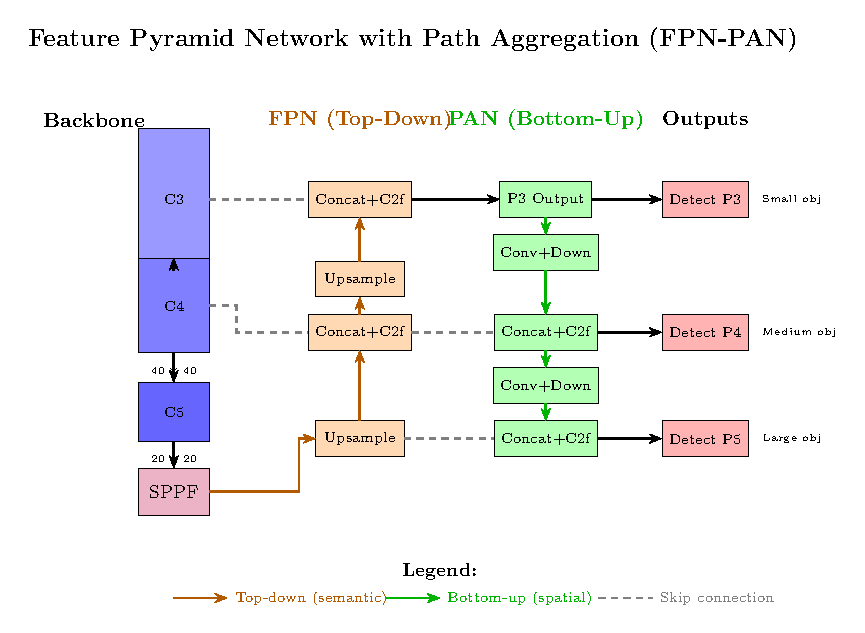
\includegraphics[width=\textwidth]{figures/ch05_fig1_fpn_pan.pdf}
\caption{Feature Pyramid Network with Path Aggregation (FPN-PAN) architecture used in YOLO models. The top-down FPN pathway propagates semantic information from deeper layers to shallower layers through upsampling, while the bottom-up PAN pathway enhances localization signals by propagating spatial information back through the network. Skip connections (dashed lines) enable direct feature reuse across scales. This bidirectional design enables effective multi-scale detection, with P3 features detecting small objects, P4 for medium objects, and P5 for large objects.}
\label{fig:fpn_pan}
\end{figure}

YOLOv5 introduced several training innovations that significantly improved practical usability, including auto-anchor computation that dynamically adjusts anchor box dimensions based on dataset statistics, cosine annealing learning rate scheduling, and comprehensive data augmentation pipelines incorporating mosaic and mixup techniques. The model family spans five size variants ranging from nano to extra-large, with YOLOv5s achieving an mAP of 37.4\% on COCO val2017 at 640 pixel resolution while maintaining inference speeds exceeding 450 frames per second on modern GPU hardware.

\subsection{YOLOv8 Improvements}

YOLOv8, released in January 2023 by Ultralytics, introduced several architectural refinements that address limitations identified in previous versions. The most significant modification involves the transition from a coupled detection head to a decoupled head architecture, separating the classification and localization branches to allow independent optimization of weights for each task. This architectural change typically leads to better convergence during training and improved accuracy, as the network can tune features specifically for identifying what an object is versus determining where it is located.

The backbone architecture in YOLOv8 replaces the C3 modules used in YOLOv5 with the more efficient C2f (Cross-Stage Partial with Two Convolutions and Fusion) module. The C2f design captures richer gradient information by incorporating additional split and concatenation operations, enhancing the model's ability to learn discriminative features while maintaining computational efficiency. This modification proves particularly beneficial when training on synthetic data, where the diversity of rendered appearances requires robust feature extraction capabilities.

\begin{figure}[htbp]
\centering
\begin{tikzpicture}[
    node distance=0.8cm and 1.2cm,
    block/.style={rectangle, draw, fill=blue!20, text width=2.2cm, text centered, minimum height=0.7cm, font=\scriptsize},
    convblock/.style={rectangle, draw, fill=green!20, text width=1.8cm, text centered, minimum height=0.6cm, font=\scriptsize},
    detectblock/.style={rectangle, draw, fill=red!20, text width=1.8cm, text centered, minimum height=0.6cm, font=\scriptsize},
    neckblock/.style={rectangle, draw, fill=orange!20, text width=1.8cm, text centered, minimum height=0.6cm, font=\scriptsize},
    arrow/.style={->, >=stealth, thick},
    dashedarrow/.style={->, >=stealth, thick, dashed}
]

% Backbone
\node[block] (input) {Input\\$640 \times 640 \times 3$};
\node[convblock, below=of input] (conv1) {Conv\\$320 \times 320$};
\node[convblock, below=of conv1] (conv2) {Conv\\$160 \times 160$};
\node[convblock, below=of conv2] (c2f1) {C2f Block\\$160 \times 160$};
\node[convblock, below=of c2f1] (conv3) {Conv\\$80 \times 80$};
\node[convblock, below=of conv3] (c2f2) {C2f Block\\$80 \times 80$};

% Side branch for P3
\node[convblock, right=1.5cm of c2f2] (conv4) {Conv\\$40 \times 40$};
\node[convblock, below=of conv4] (c2f3) {C2f Block\\$40 \times 40$};
\node[convblock, below=of c2f3] (conv5) {Conv\\$20 \times 20$};
\node[convblock, below=of conv5] (c2f4) {C2f Block\\$20 \times 20$};
\node[convblock, below=of c2f4] (sppf) {SPPF\\$20 \times 20$};

% Neck - FPN path
\node[neckblock, left=1.5cm of sppf] (upsample1) {Upsample\\$40 \times 40$};
\node[neckblock, below=of upsample1] (concat1) {Concat + C2f\\$40 \times 40$};
\node[neckblock, below=of concat1] (upsample2) {Upsample\\$80 \times 80$};
\node[neckblock, below=of upsample2] (concat2) {Concat + C2f\\$80 \times 80$};

% PAN path
\node[neckblock, right=1.5cm of concat2] (conv6) {Conv\\$40 \times 40$};
\node[neckblock, below=of conv6] (concat3) {Concat + C2f\\$40 \times 40$};
\node[neckblock, below=of concat3] (conv7) {Conv\\$20 \times 20$};
\node[neckblock, below=of conv7] (concat4) {Concat + C2f\\$20 \times 20$};

% Detection Heads
\node[detectblock, below=0.6cm of concat2] (detect1) {Detect P3\\(Small)};
\node[detectblock, below=0.6cm of concat3] (detect2) {Detect P4\\(Medium)};
\node[detectblock, below=0.6cm of concat4] (detect3) {Detect P5\\(Large)};

% Backbone arrows
\draw[arrow] (input) -- (conv1);
\draw[arrow] (conv1) -- (conv2);
\draw[arrow] (conv2) -- (c2f1);
\draw[arrow] (c2f1) -- (conv3);
\draw[arrow] (conv3) -- (c2f2);
\draw[arrow] (c2f2) -- (conv4);
\draw[arrow] (conv4) -- (c2f3);
\draw[arrow] (c2f3) -- (conv5);
\draw[arrow] (conv5) -- (c2f4);
\draw[arrow] (c2f4) -- (sppf);

% Neck arrows
\draw[arrow] (sppf) -- (upsample1);
\draw[arrow] (upsample1) -- (concat1);
\draw[arrow] (concat1) -- (upsample2);
\draw[arrow] (upsample2) -- (concat2);
\draw[arrow] (concat2) -- (conv6);
\draw[arrow] (conv6) -- (concat3);
\draw[arrow] (concat3) -- (conv7);
\draw[arrow] (conv7) -- (concat4);

% Skip connections
\draw[dashedarrow] (c2f3) -| (concat1);
\draw[dashedarrow] (c2f2) -| (concat2);
\draw[dashedarrow] (concat1) -| (concat3);
\draw[dashedarrow] (sppf) -| (concat4);

% Detection head arrows
\draw[arrow] (concat2) -- (detect1);
\draw[arrow] (concat3) -- (detect2);
\draw[arrow] (concat4) -- (detect3);

% Labels
\node[above=0.1cm of input, font=\small\bfseries] {Backbone};
\node[left=0.1cm of upsample1, font=\small\bfseries, rotate=90, anchor=south] {Neck};
\node[below=0.1cm of detect2, font=\small\bfseries] {Decoupled Heads};

\end{tikzpicture}
\caption{Simplified YOLOv8 architecture showing the backbone with C2f modules, the FPN-PAN neck structure for multi-scale feature fusion, and decoupled detection heads for three output scales. Skip connections (dashed) enable gradient flow and feature reuse across scales.}
\label{fig:yolov8_architecture}
\end{figure}

YOLOv8 also transitions from anchor-based detection to an anchor-free approach, eliminating the need for predefined anchor boxes and simplifying the training pipeline. The anchor-free paradigm directly predicts object centers and dimensions, reducing the number of hyperparameters requiring tuning and improving generalization to objects with aspect ratios not well-represented by predefined anchors. This characteristic proves advantageous when training on synthetic data where object configurations may differ substantially from those in standard benchmark datasets.

\begin{figure}[htbp]
\centering
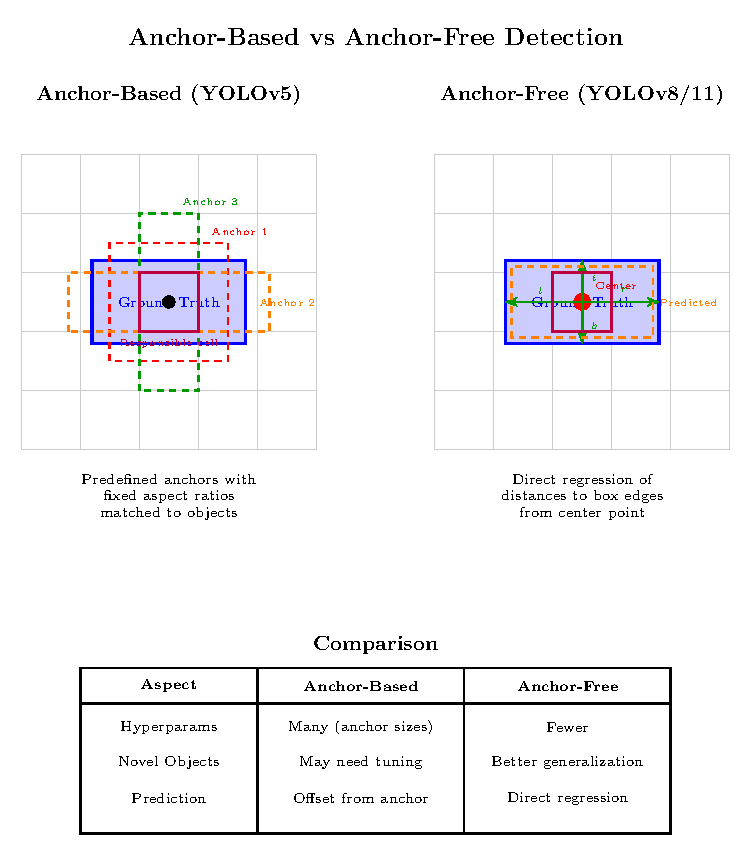
\includegraphics[width=0.95\textwidth]{figures/ch05_fig2_anchor_boxes.pdf}
\caption{Comparison of anchor-based (YOLOv5) and anchor-free (YOLOv8/YOLO11) detection paradigms. In anchor-based detection (left), predefined anchor boxes with various aspect ratios are matched to ground truth objects, and the network predicts offsets from these anchors. In anchor-free detection (right), the network directly regresses distances from the predicted center point to the four box edges ($l$, $r$, $t$, $b$), eliminating the need to predefine anchor dimensions. The anchor-free approach reduces hyperparameters and improves generalization to objects with unusual aspect ratios common in synthetic data.}
\label{fig:anchor_comparison}
\end{figure}

The loss function in YOLOv8 incorporates Distribution Focal Loss (DFL) for bounding box regression, replacing the traditional coordinate regression approach with a distribution-based formulation that models the uncertainty in localization predictions. Combined with Complete Intersection over Union (CIoU) loss for box regression and binary cross-entropy with logits for classification, the composite loss function provides stable training dynamics across diverse data distributions.

\subsection{YOLO11 Latest Features}

YOLO11, released in late 2024, represents the latest stable release in the Ultralytics YOLO family and introduces significant architectural improvements that enhance feature extraction capabilities while optimizing computational graphs. The model architecture refines the C2f module design introduced in YOLOv8, incorporating additional attention mechanisms that improve the network's ability to focus on salient image regions. These attention modules operate with minimal computational overhead, maintaining the real-time inference capabilities expected from YOLO architectures.

The backbone in YOLO11 employs enhanced spatial pyramid pooling with attention (SPPA), extending the traditional SPPF module to incorporate channel and spatial attention mechanisms. This modification improves the model's receptive field coverage while maintaining efficient memory access patterns suitable for deployment on resource-constrained devices. The neck architecture in YOLO11 introduces bi-directional feature pyramid improvements that enhance gradient flow during training, accelerating convergence when training on limited or synthetic datasets.

YOLO11 provides comprehensive task support including object detection, instance segmentation, pose estimation, oriented bounding box detection, and image classification, all within a unified framework. This versatility enables practitioners to experiment with different task formulations when developing synthetic data pipelines, potentially discovering that auxiliary tasks provide useful training signals that improve detection performance. The model maintains backward compatibility with YOLOv8 configuration files while introducing new hyperparameters for controlling the attention mechanism strength and feature fusion strategies.

\subsection{YOLO-NAS and Neural Architecture Search}

YOLO-NAS, developed by Deci AI and released in 2023, represents a fundamentally different approach to YOLO architecture design through the application of Neural Architecture Search (NAS) techniques. Rather than hand-designing architectural components, YOLO-NAS utilizes Deci's proprietary AutoNAC (Automated Neural Architecture Construction) engine to discover optimal block configurations, channel widths, and connectivity patterns for specific hardware targets and accuracy requirements.

The resulting architectures incorporate several innovations not present in manually-designed YOLO variants. YOLO-NAS introduces quantization-aware blocks (QABlocks) that maintain accuracy when the model is converted to INT8 precision through post-training quantization (PTQ). This design consideration proves valuable for edge deployment scenarios where computational resources are limited, but also benefits training pipelines by enabling mixed-precision training without requiring quantization-aware training procedures.

YOLO-NAS achieves notable improvements in small object detection performance, addressing a traditional weakness in YOLO architectures. The NAS-discovered architectures allocate additional capacity to high-resolution feature maps, improving localization accuracy for objects occupying small image regions. Performance benchmarks demonstrate a 20.5\% improvement over YOLOv7, an 11\% improvement over YOLOv5, and a 1.75\% gain compared to YOLOv8 on standard detection benchmarks.

The models come pre-trained on multiple large-scale datasets including COCO, Objects365, and Roboflow 100, providing robust feature representations that transfer effectively to downstream tasks. This extensive pre-training proves particularly valuable for synthetic-to-real transfer scenarios, as the pretrained features encode general object concepts that help bridge the domain gap between synthetic training data and real test environments. However, practitioners should note that Deci was acquired by NVIDIA in 2024, and the original development team no longer actively maintains these models, though Ultralytics continues to provide integration support.

\subsection{Architecture Comparison}

\begin{table}[htbp]
\centering
\caption{Comparison of YOLO Architecture Variants}
\label{tab:yolo_comparison}
\begin{tabular}{p{2.5cm}p{2cm}p{2cm}p{2cm}p{2cm}p{2cm}}
\toprule
\textbf{Feature} & \textbf{YOLOv5} & \textbf{YOLOv8} & \textbf{YOLO11} & \textbf{YOLO-NAS} \\
\midrule
Release Year & 2020 & 2023 & 2024 & 2023 \\
Framework & PyTorch & PyTorch & PyTorch & PyTorch \\
Backbone & CSPDarknet & CSPDarknet (C2f) & CSPDarknet (C2f+Attn) & NAS-optimized \\
Detection Head & Coupled & Decoupled & Decoupled & Decoupled \\
Anchor Type & Anchor-based & Anchor-free & Anchor-free & Anchor-free \\
mAP (COCO) & 50.7\% (v5x) & 53.9\% (v8x) & 54.7\% (11x) & 52.2\% (L) \\
Parameters (S) & 7.2M & 11.2M & 9.4M & 12.2M \\
FPS (A100) & 250 & 280 & 295 & 310 \\
PTQ Support & Limited & No & No & Native \\
Small Object & Baseline & Improved & Enhanced & Best \\
Active Maint. & Yes & Yes & Yes & Limited \\
\bottomrule
\end{tabular}
\end{table}

The architectural comparison presented in Table~\ref{tab:yolo_comparison} highlights the evolutionary trajectory of YOLO designs and the tradeoffs inherent in each variant. For synthetic-to-real training scenarios, several factors warrant particular consideration. The decoupled head architecture present in YOLOv8 and later versions provides faster convergence during fine-tuning, reducing the number of epochs required to achieve stable performance on new data distributions. The anchor-free detection paradigm simplifies training configuration by eliminating the need to tune anchor box dimensions for synthetic data that may contain objects with unusual aspect ratios.

\section{Model Selection for Synthetic Training}
\label{sec:model_selection}

\subsection{Recommendation of YOLOv8s and YOLO11s}

For synthetic-to-real training scenarios where reinforcement learning agents optimize data generation parameters, the small variants of YOLOv8 and YOLO11 (denoted YOLOv8s and YOLO11s) emerge as the recommended choices based on multiple converging factors. These models provide sufficient capacity to learn complex object representations while maintaining training times compatible with iterative optimization loops. The small variants typically require 15-30 minutes per training epoch on modern GPU hardware with datasets of a few thousand images, enabling dozens of training iterations per day within the RL optimization framework.

The YOLOv8s architecture comprises approximately 11.2 million parameters with the C2f backbone and decoupled detection head, achieving an mAP of 44.9\% on COCO val2017 at 640 pixel resolution. This performance level provides a meaningful signal for the RL agent to optimize against while avoiding the overfitting tendencies that larger models exhibit when trained on limited synthetic data. Similarly, YOLO11s offers enhanced feature extraction through its attention mechanisms while maintaining a comparable parameter count, making it suitable for scenarios where improved small object detection is critical.

Research on transfer learning with YOLO architectures demonstrates that models pre-trained on large-scale datasets like COCO significantly outperform scratch-trained models across all evaluation metrics including precision, recall, and mean Average Precision. The pretrained YOLOv8s and YOLO11s models provide feature representations that encode general object concepts, substantially reducing the amount of synthetic data required to achieve acceptable detection performance. This pretraining benefit proves essential when operating within the computational constraints of RL-guided optimization, where training data volume per iteration must remain bounded.

\subsection{Pretrained Backbone Considerations}

The decision to utilize pretrained backbones versus training from scratch fundamentally impacts the synthetic-to-real transfer performance and the efficiency of the overall optimization pipeline. Pretrained backbones, typically initialized with weights learned on the COCO dataset containing 80 object categories and over 200,000 labeled images, provide feature extractors that have learned to identify edges, textures, shapes, and semantic patterns that generalize across visual domains. When fine-tuning on synthetic data, these pretrained features serve as a strong regularization mechanism, constraining the model to representations that transfer well to real images.

The COCO-pretrained weights encode hierarchical visual features ranging from low-level edge detectors in early layers to high-level semantic concept detectors in deeper layers. When the synthetic training data shares similar low-level visual features with real images (common edges, textures, and color distributions), freezing early backbone layers during training preserves these transferable features while allowing later layers to adapt to domain-specific patterns. This selective freezing strategy proves particularly effective when synthetic data exhibits domain shift in high-level appearance characteristics but maintains realistic low-level statistics.

For novel object categories not present in COCO, the pretrained backbone still provides valuable initialization by encoding general feature extraction capabilities. Research demonstrates that pretrained models converge faster and achieve better final performance even when target categories differ entirely from pretraining categories, suggesting that the learned feature representations capture fundamental visual patterns rather than category-specific templates. When training on synthetic data depicting specialized objects, starting from pretrained weights reduces the risk of learning synthetic-specific artifacts that do not transfer to real images.

\subsection{Model Size Tradeoffs}

The YOLO model family provides variants spanning a wide range of computational requirements, from nano models suitable for embedded deployment to extra-large models targeting maximum accuracy. Understanding the tradeoffs between model sizes enables informed selection for synthetic training scenarios where iteration speed and detection performance must be balanced.

Nano variants (YOLOv8n, YOLO11n) containing approximately 3 million parameters offer the fastest training times, typically completing epochs in under 10 minutes on consumer GPU hardware. These models suit exploratory phases of RL optimization where rapid iteration across diverse parameter configurations takes priority over absolute detection accuracy. However, nano models exhibit limited capacity to capture fine-grained appearance variations, potentially providing noisy reward signals that complicate RL agent learning. The shallow feature hierarchies in nano models also show reduced robustness to domain shift, limiting their effectiveness for synthetic-to-real transfer without extensive real data fine-tuning.

Small variants (YOLOv8s, YOLO11s) strike an effective balance between training efficiency and detection capability. With roughly 10 million parameters, these models provide sufficient representational capacity to learn discriminative features from diverse synthetic data while maintaining training times compatible with iterative optimization. Small models demonstrate good transfer learning performance, benefiting substantially from pretrained initialization while remaining adaptable to synthetic domain characteristics.

Medium variants (YOLOv8m, YOLO11m) with approximately 25 million parameters offer improved detection accuracy, particularly for challenging cases involving small objects, occlusion, or unusual viewpoints. The increased capacity enables these models to memorize more training examples, which can be beneficial when synthetic data contains high diversity in object appearances and scene configurations. However, the larger parameter count increases susceptibility to overfitting on limited synthetic data, requiring careful regularization and data augmentation to maintain generalization to real images.

Large and extra-large variants (YOLOv8l/x, YOLO11l/x) containing 40-70 million parameters achieve state-of-the-art accuracy on benchmark datasets but present significant challenges for synthetic training scenarios. Training times increase substantially, reducing the number of iterations possible within RL optimization budgets. More critically, these large models require extensive training data to avoid overfitting, typically exceeding the few thousand images practical for synthetic generation pipelines. Unless real-time inference constraints demand the absolute highest accuracy and computational resources are abundant, practitioners should generally prefer small or medium variants for synthetic-to-real training pipelines.

\subsection{Transfer Learning from COCO}

Transfer learning from COCO-pretrained weights represents the recommended initialization strategy for YOLO models trained on synthetic data. The COCO dataset's diversity encompassing 80 object categories across natural scenes, urban environments, and indoor settings provides feature representations that generalize effectively to most target domains. Research comparing models trained from scratch versus those pre-trained on COCO consistently demonstrates that pretrained models achieve higher accuracy with fewer training epochs, faster convergence, and improved robustness to distribution shift between training and test data.

The transfer learning process involves loading pretrained weights for the backbone and neck components while randomly initializing the detection head layers responsible for category-specific predictions. This partial transfer approach preserves general feature extraction capabilities while allowing the detection head to specialize for target categories present in the synthetic training data. When target categories overlap with COCO categories, practitioners may optionally transfer detection head weights as well, further accelerating convergence and improving final performance.

Fine-tuning pretrained models requires careful learning rate selection to balance adaptation to new data distributions against preservation of transferable features. Research indicates that learning rates approximately 10 times lower than those used for training from scratch provide effective fine-tuning, allowing gradual weight updates that preserve pretrained knowledge while accommodating domain-specific patterns. The cosine annealing learning rate schedule employed by default in YOLO training automatically reduces learning rates during training, providing natural regularization that prevents overfitting to synthetic data characteristics.

\section{Training Configuration for RL Feedback Loops}
\label{sec:training_config}

\begin{figure}[htbp]
\centering
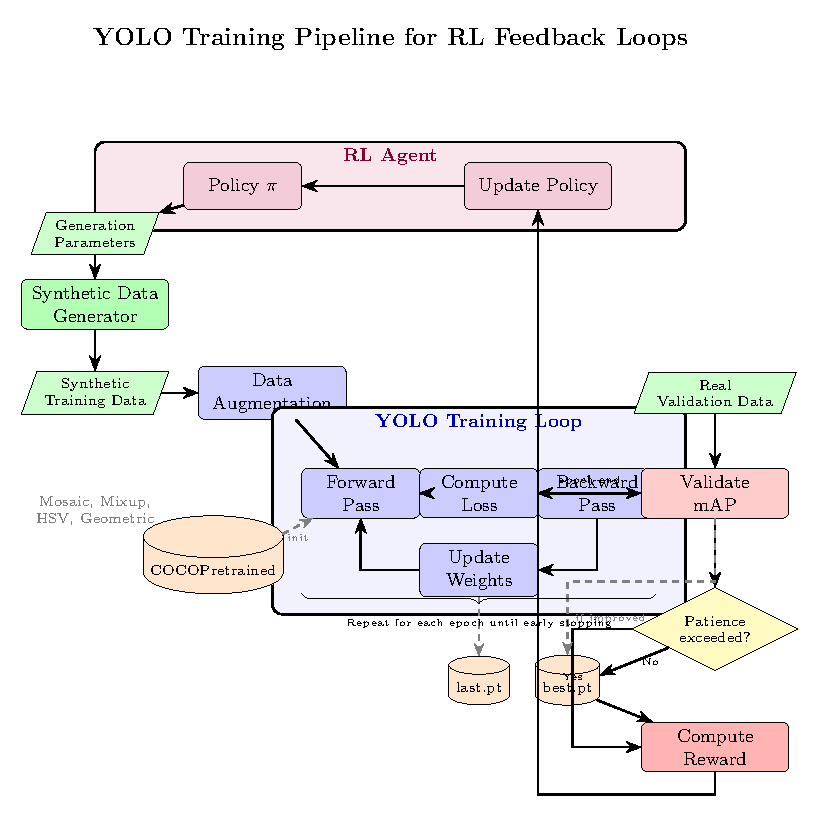
\includegraphics[width=0.95\textwidth]{figures/ch05_fig3_training_pipeline.pdf}
\caption{YOLO training pipeline integrated with reinforcement learning feedback loops for synthetic data optimization. The RL agent's policy generates parameters that control synthetic data generation. Generated training data undergoes augmentation (mosaic, mixup, HSV jittering, geometric transforms) before feeding into the YOLO training loop. Training proceeds with mixed precision (AMP) and early stopping based on validation mAP computed on real images. The best checkpoint (best.pt) is used to compute the reward signal that updates the RL policy, enabling iterative optimization of synthetic data generation parameters.}
\label{fig:training_pipeline}
\end{figure}

\subsection{Hyperparameter Settings for Fast Iteration}

Configuring YOLO training for integration within reinforcement learning feedback loops requires balancing training thoroughness against iteration speed. The RL agent learns to optimize synthetic data generation parameters by observing detection performance on real validation images, necessitating training runs that complete quickly enough to enable meaningful exploration of the parameter space while providing sufficiently accurate performance estimates to guide optimization.

\begin{table}[htbp]
\centering
\caption{Recommended Hyperparameters for RL-Integrated Training}
\label{tab:hyperparameters}
\begin{tabular}{p{3.5cm}p{2.5cm}p{6cm}}
\toprule
\textbf{Parameter} & \textbf{Value} & \textbf{Rationale} \\
\midrule
epochs & 50-100 & Sufficient for convergence with early stopping \\
batch & 16-32 & Balance GPU utilization and gradient noise \\
imgsz & 640 & Standard resolution balancing detail and speed \\
lr0 & 0.01 & Initial learning rate for pretrained models \\
lrf & 0.01 & Final LR ratio for cosine annealing \\
momentum & 0.937 & SGD momentum for stable updates \\
weight\_decay & 0.0005 & L2 regularization against overfitting \\
warmup\_epochs & 3.0 & Gradual LR increase for stability \\
warmup\_momentum & 0.8 & Reduced momentum during warmup \\
box & 7.5 & Box loss gain weighting \\
cls & 0.5 & Classification loss gain \\
dfl & 1.5 & Distribution focal loss gain \\
patience & 20 & Early stopping patience epochs \\
cache & ram & Cache images in RAM for speed \\
amp & True & Enable automatic mixed precision \\
close\_mosaic & 10 & Disable mosaic in final epochs \\
\bottomrule
\end{tabular}
\end{table}

Table~\ref{tab:hyperparameters} presents recommended hyperparameter settings optimized for RL feedback loop integration. The epoch count of 50-100 provides sufficient training duration for models to converge on synthetic data while remaining bounded by early stopping when performance plateaus. Combined with a patience value of 20 epochs, this configuration automatically terminates training when validation metrics cease improving, avoiding wasted computation on converged models.

The learning rate schedule employs cosine annealing from an initial rate of 0.01 to a final ratio of 0.01 (effective final LR of 0.0001), providing gradual learning rate decay that stabilizes training in later epochs. The warmup period of 3 epochs with reduced momentum prevents unstable gradients that can occur when pretrained weights encounter substantially different data distributions, a common occurrence when training on synthetic images with domain shift from COCO.

\subsection{Batch Size Optimization}

Batch size selection significantly impacts both training dynamics and computational efficiency. Larger batch sizes improve GPU utilization by amortizing kernel launch overhead across more samples and provide more stable gradient estimates through reduced sampling variance. However, excessively large batches can reduce model generalization by limiting the exploration of the loss landscape during optimization.

For YOLO training on synthetic data, batch sizes of 16-32 typically provide optimal balance between training speed and model quality. This range maintains sufficient gradient noise to escape local minima while providing stable enough updates for reliable convergence. The batch size also affects batch normalization statistics computed during training; very small batches produce noisy statistics that degrade detection performance, motivating the avoidance of batch sizes below 8 even when GPU memory constraints apply.

The auto-batch feature available in Ultralytics YOLO implementations (specified as batch=-1) automatically determines the largest batch size that fits within available GPU memory, simplifying configuration across different hardware. However, for consistent comparison across RL iterations, fixing the batch size ensures that training dynamics remain comparable, enabling the RL agent to attribute performance differences to data generation parameters rather than training configuration variation.

\subsection{Mixed Precision Training}

Automatic Mixed Precision (AMP) training enables substantial speedups by performing forward and backward passes in FP16 precision while maintaining FP32 master weights for parameter updates. Modern GPU architectures include tensor cores optimized for FP16 matrix operations, achieving 2-8 times higher throughput compared to FP32 computation depending on the specific operation and hardware generation. For YOLO training, AMP typically provides 40-60\% reduction in training time with negligible impact on final model accuracy.

The AMP implementation in PyTorch automatically determines which operations can safely execute in reduced precision while preserving numerical stability for sensitive computations. Loss scaling techniques prevent gradient underflow that can occur when small gradient values fall below FP16 representable range, maintaining training stability across diverse data distributions. For synthetic data training where appearance statistics may differ substantially from typical natural images, the automatic loss scaling in modern AMP implementations proves essential for reliable convergence.

Enabling AMP training requires minimal configuration changes, typically involving only a single boolean flag (amp=True) in YOLO training commands. The computational savings directly translate to increased RL iteration throughput, enabling more extensive exploration of synthetic data generation parameters within fixed time budgets. Given the negligible accuracy impact and substantial speed improvements, AMP should be enabled by default for all RL-integrated training pipelines.

\subsection{Dataset Caching Strategies}

Data loading often constitutes a significant bottleneck in YOLO training pipelines, particularly when training data resides on network storage or mechanical disk drives. Each training iteration requires loading image files, parsing annotation formats, applying augmentation transforms, and transferring data to GPU memory. For RL feedback loops where the same synthetic dataset is used throughout a single training run, caching strategies that preload and retain data in memory can substantially reduce per-epoch training time.

RAM caching (cache='ram') preloads all training images into system memory during the first epoch, eliminating disk I/O for subsequent epochs. This strategy proves highly effective when dataset size fits comfortably within available RAM, typically datasets under 10,000 images with 640x640 resolution consuming approximately 10-15 GB of memory. For the few-thousand image synthetic datasets typical in RL optimization scenarios, RAM caching provides 2-3x speedup in training throughput after the initial loading phase.

Disk caching (cache='disk') creates preprocessed image files in a local cache directory, avoiding repeated decoding and initial preprocessing while maintaining lower memory requirements than RAM caching. This strategy suits scenarios where RAM is constrained but fast local storage is available, such as training on systems with NVMe SSDs. The cache persists across training runs, providing benefits for repeated training on the same synthetic dataset during RL hyperparameter tuning or ablation studies.

For dynamically generated synthetic data where each RL iteration produces new training images, neither caching strategy provides direct benefits since data changes between training runs. However, caching remains valuable during individual training runs when data augmentation creates multiple views of each source image. Practitioners should ensure cache invalidation when synthetic data generation parameters change, avoiding stale cached data that does not reflect current RL agent decisions.

\subsection{Layer Freezing Techniques}

Layer freezing during transfer learning allows practitioners to preserve pretrained features in early network layers while adapting later layers to target domain characteristics. Research on YOLO architectures demonstrates that freezing the first four backbone blocks or the complete backbone can reduce GPU memory usage by up to 28\% while maintaining or improving detection accuracy compared to full fine-tuning. This efficiency gain directly benefits RL feedback loops by reducing per-iteration training time and enabling larger batch sizes within fixed memory budgets.

The effectiveness of layer freezing depends on the relationship between source domain (COCO natural images) and target domain (synthetic rendered images) characteristics. When synthetic data maintains realistic low-level visual features including appropriate edge profiles, texture statistics, and color distributions, freezing early layers preserves effective feature extractors that transfer directly to real test images. Conversely, when synthetic data exhibits substantial low-level distribution shift (e.g., perfect edges without anti-aliasing, unrealistic textures, or limited color variation), freezing early layers can impair adaptation by preventing the network from learning domain-appropriate feature detectors.

The freeze parameter in YOLO training accepts either an integer specifying the number of layers to freeze or a list of layer indices for selective freezing. Setting freeze=10 freezes the first 10 modules (typically the backbone layers) while allowing the neck and head to adapt freely. For synthetic-to-real transfer, starting with backbone freezing and unfreezing layers if validation performance plateaus provides a practical heuristic that reduces training time while maintaining adaptation capability.

Gradual unfreezing strategies offer additional control over the transfer learning process. Beginning training with more layers frozen and progressively unfreezing layers as training progresses allows the network to first adapt high-level features in detection heads before modifying intermediate representations. This approach proves particularly effective when limited real validation data is available to guide training, as it reduces the risk of catastrophic forgetting of pretrained features early in training when optimization signals are noisy.

\begin{algorithm}[htbp]
\caption{YOLO Training Loop with Early Stopping for RL Integration}
\label{alg:training_loop}
\begin{algorithmic}[1]
\Require Synthetic training dataset $\mathcal{D}_{syn}$, Real validation dataset $\mathcal{D}_{val}$
\Require Pretrained model weights $\theta_0$, Maximum epochs $E_{max}$, Patience $P$
\Require Learning rate schedule $\eta(e)$, Loss function $\mathcal{L}$
\Ensure Trained model weights $\theta^*$, Best validation mAP $m^*$

\State Initialize model with pretrained weights: $\theta \leftarrow \theta_0$
\State Initialize best metrics: $m^* \leftarrow 0$, $e^* \leftarrow 0$
\State Initialize early stopping counter: $c \leftarrow 0$
\State Cache training dataset in RAM if memory permits
\State Enable automatic mixed precision (AMP)

\For{epoch $e = 1$ to $E_{max}$}
    \State Set learning rate: $\eta \leftarrow \eta(e)$
    \If{$e > E_{max} - 10$}
        \State Disable mosaic augmentation \Comment{close\_mosaic}
    \EndIf

    \For{each batch $\mathcal{B} \in \mathcal{D}_{syn}$}
        \State Apply augmentation (mosaic, mixup, HSV jitter, geometric)
        \State Forward pass with AMP: $\hat{y} \leftarrow f_\theta(\mathcal{B})$
        \State Compute loss: $L \leftarrow \mathcal{L}(\hat{y}, y)$ \Comment{CIoU + BCE + DFL}
        \State Backward pass with gradient scaling
        \State Update weights: $\theta \leftarrow \theta - \eta \nabla_\theta L$
    \EndFor

    \State Evaluate on validation set: $m \leftarrow \text{mAP}(f_\theta, \mathcal{D}_{val})$

    \If{$m > m^*$}
        \State Update best: $m^* \leftarrow m$, $\theta^* \leftarrow \theta$, $e^* \leftarrow e$
        \State Save checkpoint: best.pt
        \State Reset counter: $c \leftarrow 0$
    \Else
        \State Increment counter: $c \leftarrow c + 1$
    \EndIf

    \If{$c \geq P$}
        \State \textbf{break} \Comment{Early stopping triggered}
    \EndIf
\EndFor

\State \Return $\theta^*$, $m^*$
\end{algorithmic}
\end{algorithm}

\section{Data Augmentation Strategies}
\label{sec:augmentation}

\subsection{Mosaic Augmentation}

Mosaic augmentation, introduced in YOLOv4, represents one of the most impactful data augmentation techniques for object detection training. The technique combines four training images into a single composite image by placing them in a 2x2 grid arrangement with randomized boundaries. This composition forces the model to detect objects in varied contexts, at different relative scales, and with diverse neighboring content, substantially improving generalization to novel scene configurations.

The mosaic technique provides several benefits particularly relevant to synthetic data training. By combining multiple synthetic images, mosaic increases the effective diversity of training batches beyond what the original dataset contains. Objects from different synthetic scenes appear together in novel combinations, reducing the risk that the model learns scene-specific correlations that do not transfer to real images. The technique also exposes the model to objects at smaller relative scales than they appear in original images, improving small object detection performance that often proves challenging in synthetic-to-real transfer.

Mosaic augmentation does introduce potential artifacts that warrant consideration. The artificial boundaries between combined images create discontinuities in scene context that do not occur in natural images. Objects appearing near mosaic boundaries may be partially occluded or placed in impossible spatial relationships with objects from adjacent quadrants. While these artifacts provide useful regularization during early training, they can interfere with learning precise spatial relationships in later training phases. The close\_mosaic parameter addresses this concern by disabling mosaic augmentation during the final epochs (typically 10), allowing the model to refine predictions on unmodified images before evaluation.

\subsection{Mixup and CutMix}

Mixup augmentation extends the linear interpolation concept from classification to object detection by blending pairs of images and their associated labels. Given two images $x_1$ and $x_2$ with corresponding detection targets $y_1$ and $y_2$, mixup creates a composite image $x' = \lambda x_1 + (1-\lambda) x_2$ with combined targets, where the mixing coefficient $\lambda$ is sampled from a Beta distribution. The blended image contains semi-transparent overlays of both source images, forcing the model to detect objects despite reduced visibility and conflicting context.

The mixup probability in YOLO training controls how frequently this augmentation applies, with typical values around 0.1-0.15 providing benefit without excessive training signal noise. Higher mixup probabilities can impair convergence by presenting predominantly blended images that lack the clear object boundaries present in real test images. For synthetic-to-real transfer, moderate mixup helps the model develop robustness to appearance variations while maintaining sensitivity to the distinct object features necessary for accurate detection.

CutMix presents a related but distinct augmentation approach that pastes rectangular patches from one image onto another rather than blending pixel values. The pasted patch brings objects from the source image into novel contexts, increasing effective training diversity. Unlike mixup, CutMix preserves sharp object boundaries within the pasted region while creating artificial boundaries at patch edges. This preservation of local structure may better suit detection tasks where boundary precision impacts localization accuracy.

\subsection{Color Jittering and HSV Augmentation}

Color-based augmentations modify the chromatic appearance of training images to improve model robustness against illumination variation and color distribution shift. The HSV (Hue, Saturation, Value) color space provides intuitive controls for these modifications, allowing independent adjustment of color tone, intensity, and brightness. YOLO training configurations specify HSV augmentation through three parameters controlling the maximum perturbation in each dimension: hsv\_h for hue shift (typically 0.015), hsv\_s for saturation scaling (typically 0.7), and hsv\_v for value scaling (typically 0.4).

For synthetic-to-real transfer, HSV augmentation proves particularly valuable when synthetic rendering produces color distributions that differ from real image statistics. Common rendering artifacts include oversaturated colors, limited dynamic range, and unrealistic lighting that produces uniform illumination without natural gradients. HSV augmentation applied during training exposes the model to broader color variation than present in synthetic data alone, improving generalization to the diverse lighting conditions encountered in real images.

The magnitude of HSV augmentation requires careful tuning for synthetic data scenarios. Excessive color perturbation can create unrealistic training examples that degrade model performance, while insufficient augmentation fails to bridge the color distribution gap between synthetic and real domains. Practitioners should examine representative synthetic images alongside target real images to calibrate appropriate augmentation ranges, ensuring that augmented synthetic images span the color distribution observed in real validation data.

\subsection{Geometric Augmentations}

Geometric augmentations modify the spatial arrangement of image content through transformations including scaling, rotation, translation, shearing, and perspective warping. These augmentations improve model invariance to viewpoint variation and object positioning, critical capabilities for detection tasks where objects appear at diverse orientations and scales.

Scale augmentation (controlled by the scale parameter, typically 0.5) randomly zooms into or out of training images, presenting objects at sizes different from their original capture. This augmentation proves essential when synthetic data generation produces objects at consistent scales that do not match the scale distribution in real test images. Training with scale augmentation ensures the model learns to detect objects across the full range of sizes it will encounter during deployment.

Rotation, translation, and shearing augmentations introduce additional viewpoint variation that complements synthetic data diversity. The degrees parameter controls maximum rotation angle (typically 0.0 for detection to preserve bounding box alignment), while translate (typically 0.1) and shear (typically 0.0) control respective transformation magnitudes. For synthetic-to-real transfer where viewpoint distribution differs between domains, these augmentations help bridge the gap by exposing the model to transformations intermediate between synthetic rendering viewpoints and real image perspectives.

Horizontal flipping (fliplr, typically 0.5) provides viewpoint augmentation with no distortion cost, effectively doubling effective dataset size when objects lack strong lateral asymmetry. Vertical flipping (flipud, typically 0.0 for natural images) applies less frequently as most natural scenes have consistent up-down orientation. These augmentations should match expected real image orientations; training with vertical flips when test images maintain consistent orientation can degrade performance by learning spurious vertical invariance.

\subsection{When to Disable Augmentation}

While data augmentation generally improves model generalization, certain training phases and scenarios benefit from reduced or disabled augmentation. The close\_mosaic parameter in YOLO training automatically disables mosaic augmentation during the final epochs (default 10), allowing the model to refine predictions on unmodified images. This transition removes the artificial context discontinuities introduced by mosaic, enabling more precise localization learning before final evaluation.

For synthetic data training in RL feedback loops, augmentation strategy may vary based on optimization phase. During early RL iterations when exploring diverse data generation parameters, aggressive augmentation helps prevent overfitting to specific synthetic data characteristics. As the RL agent converges toward optimal generation parameters, reduced augmentation allows the detector to learn more precisely from the refined synthetic data, potentially improving the accuracy of reward signals used for final parameter selection.

Validation and test evaluation should always proceed without augmentation to provide consistent performance metrics. The augmented training images do not represent realistic test conditions, and applying augmentation during evaluation would introduce variance that obscures true model capability. YOLO implementations automatically disable augmentation for validation, but practitioners should verify this behavior when using custom evaluation scripts or integrating with RL reward computation.

\section{Loss Functions in YOLO}
\label{sec:loss_functions}

\subsection{Classification Loss}

Classification loss in YOLO architectures measures the accuracy of object category predictions, guiding the network to correctly identify detected objects. Modern YOLO versions employ Binary Cross-Entropy (BCE) loss with logits for multi-label classification, treating each category as an independent binary classification problem. This formulation naturally handles scenarios where a single detection might plausibly belong to multiple related categories, though YOLO datasets typically assign single labels to each ground truth box.

The BCE loss for classification is computed as:
\begin{equation}
\mathcal{L}_{cls} = -\frac{1}{N} \sum_{i=1}^{N} \left[ y_i \log(\sigma(p_i)) + (1-y_i) \log(1-\sigma(p_i)) \right]
\end{equation}
where $N$ is the number of predictions, $y_i$ is the ground truth label, $p_i$ is the predicted logit, and $\sigma$ denotes the sigmoid function. This loss provides strong gradients for both confident incorrect predictions and uncertain correct predictions, driving the model toward high-confidence accurate classifications.

Focal Loss offers an alternative classification loss formulation that addresses class imbalance by down-weighting well-classified examples. The focal loss modifies BCE by multiplying with a modulating factor $(1-p_t)^\gamma$ where $p_t$ is the predicted probability for the correct class and $\gamma$ is a focusing parameter typically set to 2. This modification reduces the loss contribution from easy examples that the model already classifies correctly, focusing learning on hard examples that require additional refinement.

For synthetic-to-real training, the classification loss behavior warrants particular attention. Synthetic data may present object appearances with less variation than real data, leading to overconfident predictions that do not generalize. Monitoring classification confidence calibration on real validation data during training helps identify this issue; if synthetic-trained models produce high-confidence incorrect predictions on real images, increased regularization or focal loss application may improve transfer performance.

\subsection{Localization Loss Evolution}

Bounding box regression loss has evolved substantially across YOLO versions, progressing from simple coordinate regression to sophisticated intersection-based formulations. Early YOLO versions employed Mean Squared Error (MSE) loss on box coordinates, directly penalizing Euclidean distance between predicted and ground truth box parameters. While computationally simple, MSE loss does not directly optimize the evaluation metric (Intersection over Union) and weights coordinate errors independently of their impact on box overlap.

\begin{figure}[htbp]
\centering
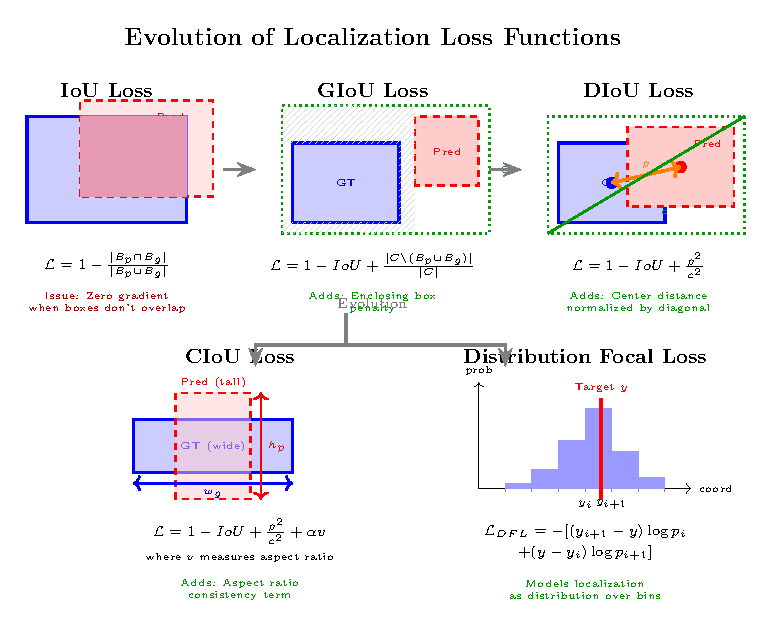
\includegraphics[width=\textwidth]{figures/ch05_fig4_iou_losses.pdf}
\caption{Evolution of localization loss functions in object detection. IoU loss directly optimizes box overlap but provides zero gradients for non-overlapping boxes. GIoU addresses this by penalizing empty space within the enclosing box $C$. DIoU explicitly minimizes center point distance $\rho$ normalized by the diagonal $c$ of the enclosing box. CIoU further adds an aspect ratio consistency term $\alpha v$ to encourage matching box shapes. Distribution Focal Loss (DFL) reformulates coordinate regression as classification over discretized bins, naturally modeling localization uncertainty. Modern YOLO architectures combine CIoU with DFL for robust localization learning.}
\label{fig:iou_losses}
\end{figure}

Intersection over Union (IoU) loss directly optimizes the overlap ratio between predicted and ground truth boxes:
\begin{equation}
\mathcal{L}_{IoU} = 1 - \frac{|B_p \cap B_g|}{|B_p \cup B_g|}
\end{equation}
where $B_p$ and $B_g$ denote predicted and ground truth boxes respectively. IoU loss provides gradients that improve box overlap regardless of the specific coordinate parameterization, but suffers from zero gradient when boxes do not overlap, preventing learning from non-overlapping predictions.

Generalized IoU (GIoU) addresses the non-overlapping gradient issue by incorporating the smallest enclosing box $C$ that contains both prediction and ground truth:
\begin{equation}
\mathcal{L}_{GIoU} = 1 - IoU + \frac{|C \setminus (B_p \cup B_g)|}{|C|}
\end{equation}
The additional term penalizes predictions that, while non-overlapping with ground truth, leave large empty regions within the enclosing box. GIoU provides gradients for all prediction-target pairs regardless of overlap, improving training stability for synthetic data that may produce detection initializations far from ground truth.

Distance IoU (DIoU) explicitly considers the normalized distance between box centers:
\begin{equation}
\mathcal{L}_{DIoU} = 1 - IoU + \frac{\rho^2(b_p, b_g)}{c^2}
\end{equation}
where $\rho(b_p, b_g)$ is the Euclidean distance between predicted and ground truth box centers, and $c$ is the diagonal length of the enclosing box. DIoU provides stronger gradients for center alignment, accelerating convergence compared to GIoU.

\subsection{Complete IoU and Shape-Aware IoU}

Complete IoU (CIoU) extends DIoU by additionally considering aspect ratio consistency between predicted and ground truth boxes:
\begin{equation}
\mathcal{L}_{CIoU} = 1 - IoU + \frac{\rho^2(b_p, b_g)}{c^2} + \alpha v
\end{equation}
where $v$ measures aspect ratio consistency and $\alpha$ is a balancing parameter. The aspect ratio term encourages predictions to match ground truth box shapes, improving localization accuracy for elongated or compact objects. CIoU serves as the default localization loss in YOLOv8 and subsequent versions, providing robust training dynamics across diverse object configurations.

Shape-aware IoU (SIoU) introduces additional terms accounting for angle cost (direction of center displacement), distance cost, and shape cost, providing more comprehensive geometric supervision. SIoU considers the angle between the line connecting box centers and the horizontal axis, encouraging predictions to approach ground truth from geometrically consistent directions. While more complex to compute, SIoU can improve convergence speed and final accuracy for challenging object configurations.

For synthetic-to-real transfer, the choice of localization loss affects how the model interprets box regression errors in synthetic data. CIoU provides a balanced formulation suitable for most scenarios, while SIoU may benefit applications where synthetic data contains objects with distinctive geometric properties (elongated shapes, specific orientations) that should transfer to real detections.

\subsection{Distribution Focal Loss}

Distribution Focal Loss (DFL), introduced in the DAMO-YOLO and incorporated into YOLOv8, reformulates bounding box regression as a classification problem over discretized coordinate distributions. Rather than directly predicting box coordinates, DFL predicts probability distributions over quantized coordinate values, with the final coordinate computed as the expected value of the distribution.

The DFL formulation addresses fundamental limitations of direct coordinate regression. When ground truth coordinates lie between discretization bins, the model must produce a distribution that, in expectation, yields the correct coordinate. This requirement naturally encourages the model to express uncertainty in localization through broader distributions while producing sharp distributions for confidently localized objects.

The DFL is computed as:
\begin{equation}
\mathcal{L}_{DFL} = -[(y_{i+1} - y) \log(p_i) + (y - y_i) \log(p_{i+1})]
\end{equation}
where $y$ is the target coordinate, $y_i$ and $y_{i+1}$ are adjacent discretization points such that $y_i \leq y \leq y_{i+1}$, and $p_i$, $p_{i+1}$ are predicted probabilities for those points. This formulation provides smooth gradients that encourage accurate distribution predictions.

For synthetic data training, DFL offers potential benefits in expressing localization uncertainty. When synthetic objects have appearance features that ambiguously localize boundaries (e.g., simple rendered shapes without detailed textures), the distribution-based formulation allows the model to predict broad distributions reflecting this ambiguity. During real image evaluation, these uncertainty estimates may improve detection reliability by down-weighting ambiguous predictions.

\subsection{Loss Function Configuration}

The composite loss function in YOLO combines classification, localization, and distribution losses with configurable weighting:
\begin{equation}
\mathcal{L}_{total} = \lambda_{box} \mathcal{L}_{CIoU} + \lambda_{cls} \mathcal{L}_{BCE} + \lambda_{dfl} \mathcal{L}_{DFL}
\end{equation}
where $\lambda_{box}$, $\lambda_{cls}$, and $\lambda_{dfl}$ control the relative importance of each component. Default YOLOv8 values of 7.5, 0.5, and 1.5 respectively emphasize localization accuracy while maintaining sufficient classification and distribution learning signals.

Adjusting loss weights can tune model behavior for specific synthetic-to-real transfer requirements. Increasing the classification weight $\lambda_{cls}$ encourages the model to focus on discriminating between object categories, beneficial when synthetic data contains objects with ambiguous appearances that might be confused. Reducing the box weight $\lambda_{box}$ may help when synthetic object boundaries differ systematically from real object boundaries, allowing the model to learn classification features more strongly while treating localization as secondary.

\section{Early Stopping and Convergence}
\label{sec:early_stopping}

\subsection{Patience-Based Early Stopping}

Early stopping provides automatic training termination when model performance on held-out validation data ceases to improve. The patience parameter specifies the number of consecutive epochs without improvement that triggers training termination. For YOLO training, patience values of 20-50 epochs typically provide appropriate balance between avoiding premature termination during temporary performance plateaus and preventing excessive computation after convergence.

The early stopping criterion monitors the primary validation metric, typically mAP@0.5 (mean Average Precision at IoU threshold 0.5) or mAP@0.5:0.95 (averaged across IoU thresholds from 0.5 to 0.95). When synthetic data characteristics differ substantially from real validation data, the validation mAP trajectory may exhibit more variability than typical same-domain training, motivating slightly increased patience values to distinguish genuine convergence from noisy performance fluctuations.

Implementation of early stopping requires maintaining the best-performing model checkpoint throughout training. Each time validation performance improves, the current model weights save to disk (typically as best.pt) and the patience counter resets. When patience epochs pass without improvement, training terminates and the best checkpoint provides the final model. This checkpoint-based approach ensures that the returned model represents peak validation performance even if training continued past the optimal epoch.

\subsection{Validation Frequency Optimization}

The frequency of validation evaluation impacts both training throughput and early stopping sensitivity. Default YOLO configurations evaluate validation performance after each training epoch, providing fine-grained monitoring of learning progress. However, each validation pass incurs computational overhead that extends total training time, particularly for large validation sets or complex evaluation metrics.

For RL feedback loops where training iteration speed is critical, reducing validation frequency can accelerate training while maintaining meaningful early stopping behavior. Evaluating every 5 or 10 epochs rather than every epoch reduces validation overhead proportionally while still capturing the general trajectory of performance improvement. The tradeoff involves potentially continuing training slightly past the optimal stopping point when the best epoch falls between validation evaluations.

The small real validation sets (approximately 50 images) typical in synthetic-to-real scenarios enable rapid validation evaluation, often completing in seconds compared to minutes-long training epochs. In these scenarios, per-epoch validation provides negligible overhead while maximizing the precision of early stopping decisions. Practitioners should profile validation time relative to epoch duration to inform frequency optimization decisions.

\subsection{Checkpoint Strategies}

Checkpoint management strategies determine which model states persist during training and how storage resources allocate across the training run. YOLO training by default maintains two checkpoint files: last.pt containing the most recent epoch's weights, and best.pt containing the weights from the epoch achieving highest validation performance. This dual-checkpoint approach ensures access to both the convergence endpoint and the peak-performance state.

For RL integration, the best.pt checkpoint provides the natural model state for reward computation, as it represents the maximum detection capability achieved during training on the current synthetic data. Computing RL rewards based on best.pt performance rather than final epoch performance ensures that temporary training instabilities or overfitting in later epochs do not corrupt the reward signal used for synthetic data optimization.

Extended checkpoint histories recording weights from multiple epochs enable post-hoc analysis of training dynamics and alternative model selection criteria. Saving checkpoints every N epochs creates a trajectory of model states that can inform understanding of how synthetic data characteristics influence learning progress. However, the storage requirements for extensive checkpoint histories can become substantial for large models, motivating selective checkpoint retention based on validation performance milestones.

Resume functionality allows training to continue from saved checkpoints, enabling recovery from interruptions and extension of training beyond initial epoch budgets. When RL optimization identifies promising synthetic data configurations, extended training from checkpoints can refine detection performance beyond what initial training epochs achieved. The resume capability requires preserving optimizer state alongside model weights, ensuring consistent learning rate scheduling and momentum accumulation across resumed training sessions.

\section{Practical Considerations for Reinforcement Learning Integration}

The integration of YOLO training within reinforcement learning optimization loops introduces considerations beyond standalone model development. The training pipeline must support automated execution without manual intervention, produce consistent and comparable results across iterations, and complete within time budgets compatible with meaningful parameter space exploration.

Deterministic training through fixed random seeds enables reproducible results that isolate the impact of synthetic data parameter changes from training stochasticity. Setting seeds for Python random number generation, NumPy, and PyTorch (including CUDA operations) provides reproducibility that strengthens the correlation between RL agent parameter choices and observed detection performance. However, some GPU operations remain non-deterministic even with fixed seeds, introducing residual variance that the RL algorithm must accommodate.

Automated metric logging and structured result storage facilitate RL agent access to training outcomes. YOLO training produces comprehensive logs including per-epoch loss values, validation metrics, and training configuration details. Integrating these logs with RL experiment tracking enables analysis of how synthetic data parameters influence training dynamics, potentially revealing relationships useful for warm-starting RL optimization or constraining parameter search spaces.

Hardware resource management ensures consistent training throughput across RL iterations. GPU memory allocation, data loading workers, and CPU utilization should remain stable across training runs to prevent variable iteration times that complicate RL scheduling. Containerized training environments provide isolation that maintains resource consistency regardless of system background activity.

\section{Summary}

This chapter has presented a comprehensive examination of YOLO architecture evolution and training strategies optimized for synthetic-to-real domain adaptation scenarios. The progression from YOLOv5 through YOLOv8 and YOLO11 demonstrates continuous refinement of feature extraction, detection head design, and loss function formulation that improves both accuracy and training efficiency. The small model variants, particularly YOLOv8s and YOLO11s, emerge as recommended choices for RL-guided synthetic data optimization, balancing detection capability against iteration speed requirements.

Training configuration for RL feedback loops requires careful attention to hyperparameter selection, mixed precision training, caching strategies, and layer freezing techniques that collectively determine iteration throughput. Data augmentation strategies including mosaic, mixup, and HSV jittering expand effective training diversity while the close\_mosaic mechanism ensures refined final-epoch learning on unmodified images.

The evolution of loss functions from simple coordinate regression through GIoU, DIoU, CIoU, and Distribution Focal Loss reflects deepening understanding of localization supervision requirements. Early stopping with appropriate patience values and checkpoint management enables efficient training termination while preserving peak-performance model states for RL reward computation.

Together, these architectural choices and training strategies form a comprehensive framework for deploying YOLO detectors within reinforcement learning systems that optimize synthetic data generation for real-world object detection applications.


% Chapter 6: Domain Adaptation and Sim-to-Real Transfer
\chapter{Domain Adaptation and Sim-to-Real Transfer}
\label{ch:domain_adaptation}

The deployment of deep learning models trained on synthetic data to real-world environments represents one of the most significant challenges in modern computer vision and robotics. This chapter provides a comprehensive treatment of the domain gap problem, examining both theoretical foundations and practical methodologies for bridging the divide between simulated and physical domains. The techniques presented herein form the theoretical backbone for reinforcement learning-based optimization of synthetic data generation parameters, enabling autonomous systems to achieve robust performance on real-world perception tasks without requiring extensive manually-labeled datasets.

\begin{figure}[htbp]
\centering
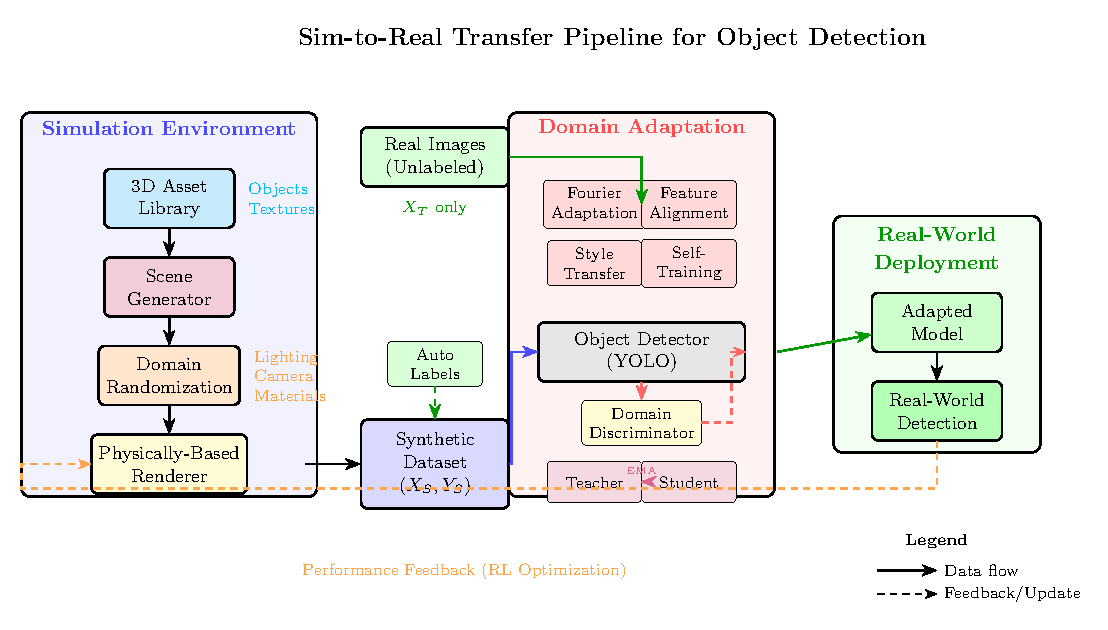
\includegraphics[width=\textwidth]{figures/ch06_fig2_simtoreal_pipeline.pdf}
\caption{Overview of the sim-to-real transfer pipeline for object detection. Synthetic data generated in simulation environments undergoes domain adaptation techniques before training object detectors. The adapted models are then deployed in real-world settings, with performance feedback potentially informing refinement of the synthetic data generation process through reinforcement learning optimization.}
\label{fig:simtoreal_pipeline}
\end{figure}

\section{The Domain Gap Problem}
\label{sec:domain_gap_problem}

The fundamental challenge of transferring knowledge from synthetic to real domains stems from distributional differences that arise from the inherent limitations of simulation environments. Understanding the mathematical formulation of this gap, its sources, and methods for quantification provides essential groundwork for developing effective mitigation strategies.

\begin{figure}[htbp]
\centering
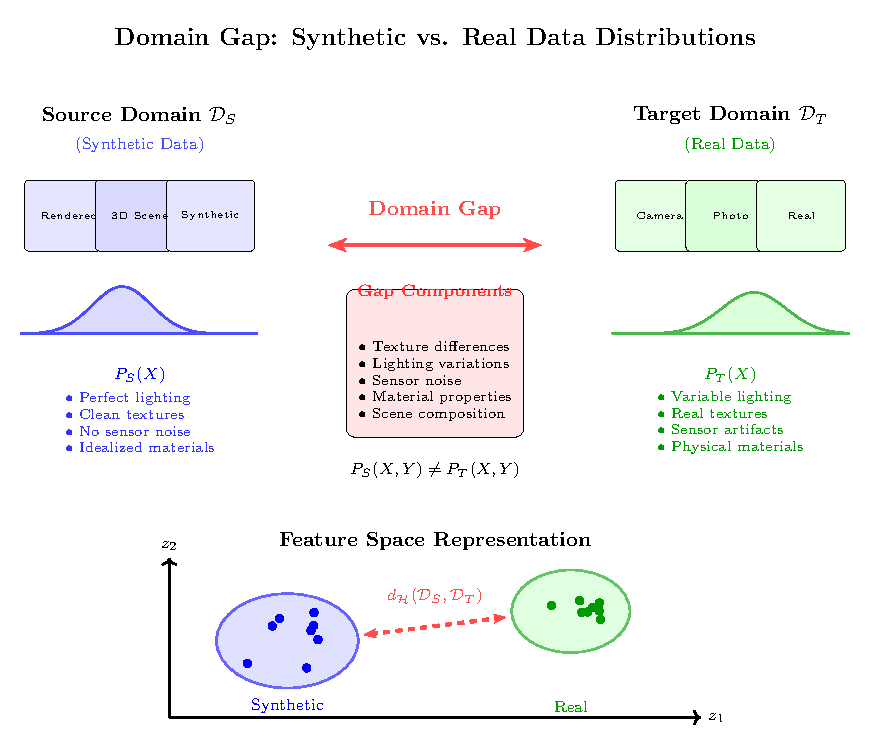
\includegraphics[width=\textwidth]{figures/ch06_fig1_domain_gap.pdf}
\caption{Visualization of the domain gap between synthetic and real data distributions. The source domain $\mathcal{D}_S$ (synthetic) and target domain $\mathcal{D}_T$ (real) exhibit different marginal distributions $P_S(X)$ and $P_T(X)$. Key gap components include texture differences, lighting variations, sensor noise characteristics, and scene composition. The bottom panel shows how this gap manifests in learned feature space, where synthetic and real samples form separated clusters with measurable distance $d_{\mathcal{H}}(\mathcal{D}_S, \mathcal{D}_T)$.}
\label{fig:domain_gap_viz}
\end{figure}

\subsection{Formal Definition of Domain Shift}

Consider a source domain $\mathcal{D}_S$ representing synthetic data and a target domain $\mathcal{D}_T$ representing real-world observations. Each domain is characterized by a joint probability distribution over input features $\mathcal{X}$ and labels $\mathcal{Y}$. The source domain distribution is denoted $P_S(X, Y)$ while the target domain distribution is $P_T(X, Y)$. Domain shift occurs when these distributions differ, mathematically expressed as $P_S(X, Y) \neq P_T(X, Y)$.

This distributional discrepancy can be decomposed into several components. Covariate shift arises when the marginal distributions differ, $P_S(X) \neq P_T(X)$, while the conditional distribution remains constant, $P_S(Y|X) = P_T(Y|X)$. Label shift occurs in the reverse scenario where $P_S(Y) \neq P_T(Y)$ but $P_S(X|Y) = P_T(X|Y)$. The most challenging case involves concept drift where both marginal and conditional distributions differ simultaneously.

\begin{definition}[Domain Gap]
\label{def:domain_gap}
Let $\mathcal{H}$ be a hypothesis class and let $h \in \mathcal{H}$ be a predictor. The domain gap $d_{\mathcal{H}}(\mathcal{D}_S, \mathcal{D}_T)$ is defined as the supremum over the hypothesis class of the difference in expected losses:
\begin{equation}
d_{\mathcal{H}}(\mathcal{D}_S, \mathcal{D}_T) = \sup_{h \in \mathcal{H}} \left| \mathbb{E}_{(x,y) \sim P_S}[\ell(h(x), y)] - \mathbb{E}_{(x,y) \sim P_T}[\ell(h(x), y)] \right|
\end{equation}
where $\ell(\cdot, \cdot)$ denotes the task-specific loss function.
\end{definition}

The implications of domain shift for object detection are particularly severe. A detector trained exclusively on synthetic renderings may exhibit dramatically degraded performance when deployed on real camera imagery due to systematic differences in texture statistics, illumination characteristics, sensor noise profiles, and contextual scene composition.

\subsection{Sources of Sim-to-Real Gap}

The discrepancy between synthetic and real visual domains originates from multiple interacting factors that span the rendering pipeline, environmental modeling, and sensor simulation. Understanding these sources enables targeted intervention strategies.

Texture fidelity represents a primary contributor to domain gap. Synthetic rendering engines, despite advances in physically-based rendering, produce texture patterns that differ systematically from real-world surface appearances. Material reflectance properties including bidirectional reflectance distribution functions are approximated rather than measured, leading to subtle but perceptually significant deviations. Research by Geirhos et al. demonstrated that convolutional neural networks exhibit strong texture bias, relying on local texture patterns for classification rather than global shape information. This bias amplifies the impact of texture discrepancies between domains, as networks trained on synthetic textures may fail to recognize objects with different but semantically equivalent surface appearances.

Illumination modeling introduces systematic biases through simplified light transport simulation. Real-world scenes exhibit complex interreflection, subsurface scattering, and atmospheric effects that are computationally expensive to simulate accurately. Synthetic environments typically employ a limited number of point or area light sources with idealized emission profiles, whereas natural environments feature continuous illumination from the sky dome, diffuse inter-object reflections, and spatially varying ambient conditions. The resulting differences in shadow characteristics, highlight patterns, and overall luminance distributions contribute significantly to domain gap.

Sensor noise characteristics differ fundamentally between simulated and physical imaging systems. Real cameras exhibit spatial noise patterns arising from pixel-level variations in sensitivity, temporal noise from electronic readout circuits, and photon shot noise following Poisson statistics. Color reproduction depends on spectral response curves of physical sensors that deviate from idealized RGB filters assumed in rendering. Lens aberrations including chromatic dispersion, vignetting, and geometric distortion are present in physical optics but typically absent from synthetic rendering.

Contextual scene composition presents challenges in ensuring that synthetic environments capture the statistical regularities of real-world object arrangements. Objects in physical environments follow implicit placement rules governed by physics, human design intent, and functional relationships. Vehicles appear on roads rather than arbitrary locations; products occupy shelves in retail environments; pedestrians traverse sidewalks and crosswalks. Violating these contextual priors in synthetic data generation produces training examples that are implausible under the real-world distribution, potentially teaching detectors spurious correlations.

\subsection{Measuring Domain Gap}

Quantitative assessment of domain discrepancy enables systematic comparison of synthetic data generation strategies and provides feedback signals for optimization-based approaches. Several metrics have been proposed for measuring distributional divergence between image domains.

The Fr\'{e}chet Inception Distance provides a widely-adopted measure of distributional similarity between image collections. Given feature representations extracted from a pretrained Inception network, FID models both synthetic and real feature distributions as multivariate Gaussians and computes the Fr\'{e}chet distance between them:
\begin{equation}
\text{FID} = \|\mu_S - \mu_T\|_2^2 + \text{Tr}\left(\Sigma_S + \Sigma_T - 2(\Sigma_S \Sigma_T)^{1/2}\right)
\end{equation}
where $\mu_S, \Sigma_S$ and $\mu_T, \Sigma_T$ denote the mean vectors and covariance matrices of source and target feature distributions respectively. Lower FID values indicate greater distributional similarity. While FID correlates with human perceptual judgments of image quality, it exhibits statistical bias when computed from limited sample sizes, requiring collections of fifty thousand or more images for reliable estimation.

The Kernel Inception Distance addresses the sample efficiency limitations of FID by employing Maximum Mean Discrepancy in the feature space. KID provides an unbiased estimator that yields reliable measurements from smaller image collections:
\begin{equation}
\text{KID} = \mathbb{E}[k(\phi(x_S), \phi(x'_S))] + \mathbb{E}[k(\phi(x_T), \phi(x'_T))] - 2\mathbb{E}[k(\phi(x_S), \phi(x_T))]
\end{equation}
where $\phi(\cdot)$ denotes the Inception feature extractor and $k(\cdot, \cdot)$ is a polynomial or Gaussian kernel function. The unbiased nature of KID makes it particularly suitable for iterative optimization scenarios where computational constraints limit the number of synthetic images generated per evaluation.

Maximum Mean Discrepancy provides a general framework for comparing probability distributions in reproducing kernel Hilbert spaces. Given kernel function $k$, the squared MMD between distributions $P$ and $Q$ is:
\begin{equation}
\text{MMD}^2(P, Q) = \left\| \mathbb{E}_{x \sim P}[\phi(x)] - \mathbb{E}_{y \sim Q}[\phi(y)] \right\|_{\mathcal{H}}^2
\end{equation}
where $\phi$ maps samples to the RKHS induced by kernel $k$. MMD can be computed efficiently using kernel evaluations without explicit feature mapping, enabling application to high-dimensional image distributions.

The Style Embedding Distribution Discrepancy metric specifically targets the synthetic-real gap by modeling domain differences as style variations. SEDD extracts style representations using Gram matrices of intermediate convolutional features and measures discrepancy through a learned embedding space optimized for intra-class compactness and inter-class separation. This approach captures texture and appearance statistics that are particularly relevant for sim-to-real transfer.

\subsection{Feature Space Analysis Methods}

Beyond scalar metrics, visualization and analysis of learned feature representations provide insight into the geometric structure of domain gap in representation space.

t-distributed Stochastic Neighbor Embedding enables projection of high-dimensional feature vectors to two-dimensional visualizations that preserve local neighborhood structure. By extracting backbone features from both synthetic and real images and projecting them jointly via t-SNE, practitioners can visually assess the degree of domain alignment. Well-aligned domains exhibit overlapping clusters in the projected space, while substantial domain gap manifests as separated clusters corresponding to synthetic and real origins. Class-conditional visualization reveals which object categories exhibit the largest domain discrepancy, enabling targeted improvement of synthetic data generation for problematic classes.

Layer-wise analysis of feature distributions across network depth provides diagnostic information about where domain-specific information persists in learned representations. Shallow layers typically exhibit greater separation between synthetic and real features due to their sensitivity to low-level image statistics including edges, textures, and color distributions. Deeper layers ideally produce more domain-invariant representations that capture semantic content rather than domain-specific appearance. Persistent domain separation in deep layers indicates insufficient domain adaptation, suggesting the need for explicit alignment mechanisms or improved synthetic data diversity.

Principal Component Analysis of feature spaces reveals the principal directions of variation and enables quantification of how much variance is explained by domain identity versus semantic content. If the first principal components separate domains rather than semantic categories, the learned representations are dominated by domain-specific rather than task-relevant information.

\section{Domain Randomization Theory}
\label{sec:dr_theory}

Domain randomization provides a conceptually elegant approach to sim-to-real transfer by deliberately introducing variation during synthetic data generation such that the real world appears as merely another sample from the training distribution. This section establishes the theoretical foundations of domain randomization and derives conditions under which it enables successful transfer.

\subsection{Theoretical Foundations}

The seminal work of Tobin et al. established the empirical effectiveness of domain randomization for robotic manipulation, demonstrating successful transfer of neural network policies trained entirely on synthetic RGB images to physical robot systems. The core insight underlying domain randomization is that by exposing the learning system to sufficient variability in non-essential visual parameters, it is forced to learn representations that are invariant to these nuisance factors and therefore more likely to generalize to novel visual conditions including those encountered in real deployments.

Formal theoretical analysis of domain randomization was provided by subsequent work establishing mathematical foundations for understanding when and why randomization enables generalization. Consider a simulator $\mathcal{S}$ parameterized by environment parameters $\xi \in \Xi$ drawn from distribution $\rho(\xi)$. The goal is to learn a policy or predictor $\pi$ that performs well under the real-world parameter instantiation $\xi^*$.

\begin{theorem}[Domain Randomization Transfer Bound]
\label{thm:dr_transfer}
Let $\pi$ be a predictor trained on synthetic data generated with environment parameters drawn from $\rho(\xi)$. Under the assumption that $\xi^* \in \text{supp}(\rho)$ and that the learned representation $\phi$ satisfies a Lipschitz condition with constant $L_\phi$, the expected loss on the target domain is bounded by:
\begin{equation}
\mathbb{E}_{(x,y) \sim P_T}[\ell(\pi(x), y)] \leq \mathbb{E}_{\xi \sim \rho}\mathbb{E}_{(x,y) \sim P_\xi}[\ell(\pi(x), y)] + L_\phi \cdot \mathbb{E}_{\xi \sim \rho}[d(\xi, \xi^*)]
\end{equation}
where $d(\cdot, \cdot)$ measures distance in parameter space and $P_\xi$ denotes the data distribution under parameter $\xi$.
\end{theorem}

This bound reveals the fundamental tradeoff in domain randomization. Broader parameter distributions $\rho$ increase the likelihood that real-world conditions fall within support while potentially increasing the average distance term. Conversely, narrow distributions centered near presumed real-world parameters minimize distance but risk excluding actual deployment conditions from the training distribution.

\begin{figure}[htbp]
\centering
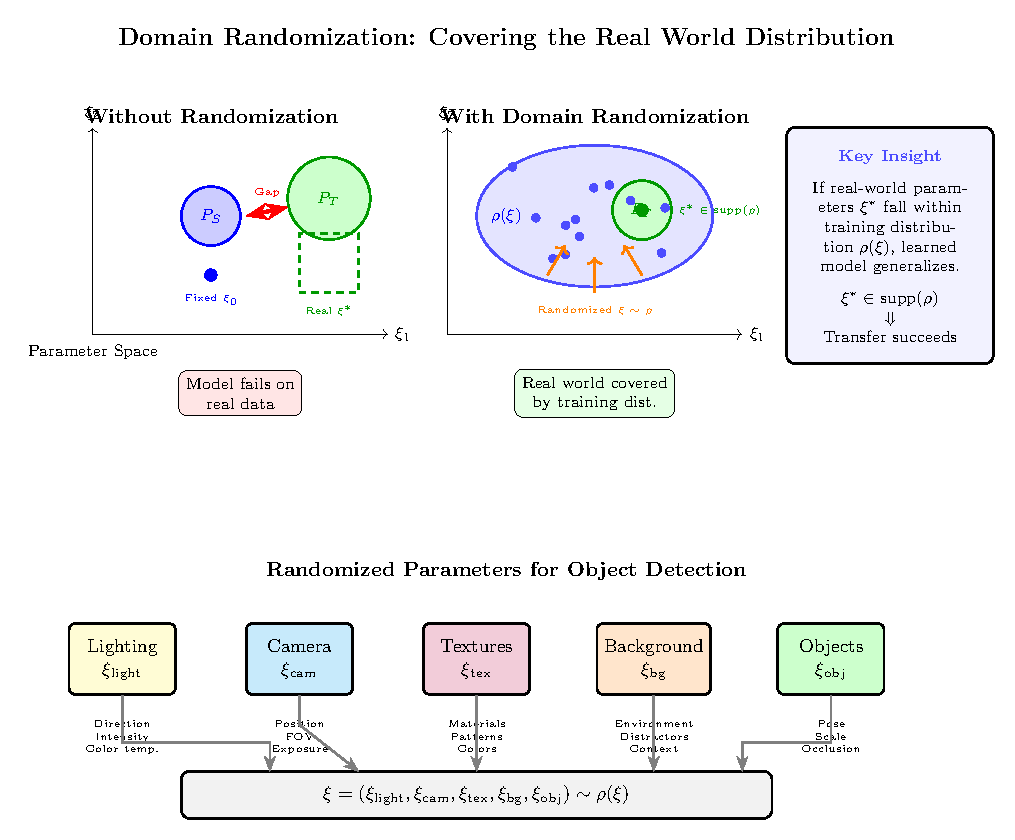
\includegraphics[width=\textwidth]{figures/ch06_fig3_domain_randomization.pdf}
\caption{The domain randomization principle for sim-to-real transfer. Without randomization (left), the narrow synthetic distribution $P_S$ fails to cover the real-world distribution $P_T$, resulting in poor transfer. With domain randomization (center), the training distribution $\rho(\xi)$ is broadened across environment parameters to encompass real-world conditions, ensuring $\xi^* \in \text{supp}(\rho)$. The bottom panel illustrates the key randomization parameters for object detection including lighting, camera pose, textures, backgrounds, and object configurations.}
\label{fig:domain_randomization}
\end{figure}

The ICLR 2022 framework for understanding domain randomization established that history-dependent policies utilizing memory or recurrence are essential for achieving tight transfer bounds. Memoryless policies cannot distinguish between environment parameters and must hedge against all possible parameter values, leading to conservative suboptimal behavior. In contrast, recurrent architectures can infer environment parameters from sequential observations and adapt their behavior accordingly, achieving near-optimal performance across the randomization distribution.

\subsection{Why Randomization Enables Generalization}

The generalization mechanism of domain randomization operates through several complementary effects on learned representations.

Invariance learning arises when parameters randomized during training are held constant within individual training episodes or images but vary across the dataset. The network cannot rely on randomized parameters for prediction since their values are unpredictable, forcing it to learn features that remain discriminative regardless of these nuisance variables. This mechanism mirrors the classical computer vision principle of designing features invariant to illumination, viewpoint, and other imaging conditions.

Distribution coverage ensures that real-world conditions fall within the training distribution when randomization ranges are sufficiently broad. From the perspective of empirical risk minimization, training on a distribution that covers the test distribution provides guarantees on generalization through standard learning theory arguments. The real world becomes just another sample from an already-observed distribution rather than an out-of-distribution extrapolation.

Regularization effects emerge from the increased training distribution entropy induced by randomization. Similar to data augmentation, domain randomization can be viewed as implicit regularization that prevents overfitting to specific visual conditions present in a narrow synthetic distribution. This regularization effect improves generalization even to conditions outside the explicit randomization ranges.

Meta-learning dynamics arise when randomization creates a distribution over distinct training environments. Memory-augmented architectures can learn to identify environment parameters from observations and adapt their processing accordingly, implementing a form of meta-learning where the network learns how to learn about new environments. This enables rapid adaptation to deployment conditions that may differ from any specific training environment.

\subsection{Optimal Randomization Ranges}

Determining appropriate ranges for randomized parameters involves balancing competing considerations. Ranges that are too narrow risk excluding real-world conditions, while excessively broad ranges increase training difficulty and may lead to overly conservative learned representations.

Empirical guidelines derived from successful applications suggest parameter-specific recommendations. Camera position should be randomized within task-relevant viewing volumes, typically spanning elevation angles from five to thirty degrees and full azimuthal coverage for objects that may be approached from any direction. Lighting parameters benefit from randomization across one to twelve light sources with log-uniform intensity distributions spanning an order of magnitude around nominal values. Background textures should be sampled from diverse image databases containing thousands of distinct patterns to ensure coverage of texture statistics encountered in deployment.

The principle of physicality constrains randomization to plausible parameter combinations. While broad marginal distributions for individual parameters may be desirable, joint distributions should respect physical constraints. Light source positions and shadow directions must be consistent. Object textures and reflectance properties should correspond to materials plausibly associated with the object category. Gravity-consistent object arrangements avoid floating or intersecting configurations that could never occur in physical environments.

Curriculum strategies for range selection begin with conservative ranges that enable initial learning and progressively expand as training progresses. This approach, formalized in automatic domain randomization methods, avoids the difficulty of learning from maximally diverse distributions while eventually achieving broad coverage.

\subsection{The Exploration-Robustness Tradeoff}

Domain randomization fundamentally trades task performance for robustness across environmental conditions. This tradeoff manifests in several ways that practitioners must navigate.

Conservative policies emerge when training under broad randomization because the learned system must hedge against all possible parameter values. A policy optimized for average performance across a wide parameter distribution will typically underperform compared to a policy specialized for specific known conditions. This suboptimality is the price paid for robustness.

Training difficulty increases with randomization breadth as the learning problem becomes more challenging. The network must simultaneously master the task and achieve invariance to randomized parameters. Combined randomization of many parameters creates a high-dimensional space of training conditions that may require substantially more training data and computational resources to cover adequately.

Diminishing returns characterize the relationship between randomization breadth and sim-to-real transfer performance. Initial randomization provides substantial benefits by breaking dependence on simulation-specific artifacts. However, beyond a threshold, additional randomization primarily increases training difficulty without proportionate gains in transfer performance, particularly when real-world conditions already fall within established ranges.

\begin{theorem}[Exploration-Robustness Tradeoff]
\label{thm:exploration_robustness}
Let $\rho_\sigma$ denote a randomization distribution with scale parameter $\sigma$ and let $R(\pi, \xi)$ denote the expected return of policy $\pi$ under environment parameter $\xi$. The robust expected return and the optimal specialized return satisfy:
\begin{equation}
\mathbb{E}_{\xi \sim \rho_\sigma}[R(\pi^*_\sigma, \xi)] \leq \max_\xi R(\pi^*_\xi, \xi) - \Omega(\sigma)
\end{equation}
where $\pi^*_\sigma$ is optimal under randomization and $\pi^*_\xi$ is optimal for specific $\xi$. The gap grows with randomization scale $\sigma$.
\end{theorem}

This theorem formalizes the intuition that robustness comes at the cost of peak performance. Practitioners must determine acceptable tradeoffs based on the relative importance of average-case versus worst-case performance in their application domain.

\section{Structured Domain Randomization}
\label{sec:structured_dr}

While uniform domain randomization provides a simple baseline, structured approaches that incorporate prior knowledge about realistic scene configurations achieve superior transfer performance with improved sample efficiency.

\subsection{NVIDIA's SDR Approach}

Structured Domain Randomization, introduced by NVIDIA researchers, represents a principled framework for incorporating contextual constraints into synthetic data generation. Rather than placing objects according to uniform distributions over spatial coordinates, SDR samples object configurations from distributions that reflect the statistical regularities of real-world scenes.

The key insight motivating SDR is that random placement of objects in arbitrary locations produces training examples that violate the implicit assumptions of real-world imagery. Vehicles appearing in the sky, pedestrians embedded in walls, and products floating above shelves represent configurations that never occur in deployment yet consume training capacity when included in uniformly randomized datasets. By restricting randomization to contextually appropriate variations, SDR focuses training on plausible configurations that better approximate the target distribution.

NVIDIA's implementation leverages semantic scene representations including ground planes, road networks, and surface normals to constrain object placement. Vehicles are instantiated on road surfaces with orientations aligned to lane directions. Pedestrians appear on sidewalks and crosswalks with standing or walking poses. Architectural elements occupy structurally appropriate positions. This context-aware placement dramatically reduces the space of generated configurations while improving relevance to real-world detection scenarios.

Empirical evaluation on autonomous driving benchmarks demonstrated that SDR achieves ten to fifteen percentage point improvements in mean average precision compared to uniform domain randomization when training detectors exclusively on synthetic data. The structured approach also exhibits improved sample efficiency, requiring fewer synthetic images to achieve comparable transfer performance.

\subsection{Context-Aware Object Placement}

Implementing context-aware placement requires explicit modeling of the spatial relationships and support structures present in target deployment environments.

Surface-based placement constrains objects to rest on appropriate supporting surfaces. Ground-contacting objects including vehicles, furniture, and pedestrians are placed such that their bases intersect ground planes or floor surfaces. Tabletop objects are positioned within the boundaries of horizontal surfaces with appropriate clearances from edges. Wall-mounted objects maintain fixed distances from vertical surfaces with orientations parallel to wall normals.

Semantic region constraints restrict object categories to appropriate spatial zones. Traffic infrastructure including signs, signals, and barriers appears within road right-of-way regions. Commercial products occupy retail fixture volumes. Office equipment populates workspace zones. These constraints encode domain knowledge about the spatial organization of target environments.

Occlusion modeling controls the visibility relationships between objects. Structured approaches can ensure minimum visibility thresholds for each object instance while permitting realistic partial occlusions. Complete occlusion, where target objects are entirely hidden behind foreground elements, wastes training examples on cases that provide no learning signal for the detection task.

Physical simulation provides a mechanism for generating gravity-consistent multi-object arrangements. Rather than placing objects at specified coordinates which may result in interpenetration, objects can be dropped into scenes under simulated physics and allowed to settle into stable configurations. This approach automatically generates realistic piles, stacks, and cluttered arrangements without explicit modeling of all possible contact configurations.

\subsection{Conditional Sampling Strategies}

Sophisticated domain randomization employs conditional sampling where the distribution over later parameters depends on values sampled for earlier parameters.

Hierarchical scene generation first samples high-level scene properties including environment type, time of day, and weather conditions, then samples object-level parameters conditioned on the scene context. An indoor warehouse scene implies different lighting distributions, object categories, and spatial scales than an outdoor urban environment. Conditioning enables generation of internally consistent scenes where all parameters reflect a coherent underlying scenario.

Correlated parameter sampling captures dependencies between physically related quantities. Light source position determines shadow direction; modifying one without the other produces physically impossible imagery. Material properties including roughness, metallicity, and index of refraction are correlated for real materials; sampling them independently produces implausible combinations. Capturing these correlations through joint or conditional distributions improves the physical plausibility of generated images.

Episodic consistency maintains constant values for scene-level parameters within individual training sequences while varying them across sequences. This approach is particularly relevant for video-based training where temporal consistency of lighting, weather, and environment identity is expected. Within-episode consistency also enables recurrent architectures to infer environment parameters from initial observations and condition subsequent processing accordingly.

\subsection{Comparison of Structured and Unstructured Domain Randomization}

The relative merits of structured and unstructured domain randomization depend on available prior knowledge, computational resources, and transfer performance requirements. Table~\ref{tab:dr_comparison} summarizes key differences between these approaches.

\begin{table}[htbp]
\centering
\caption{Comparison of Unstructured and Structured Domain Randomization Approaches}
\label{tab:dr_comparison}
\begin{tabular}{p{3.5cm}p{5.5cm}p{5.5cm}}
\toprule
\textbf{Characteristic} & \textbf{Unstructured DR} & \textbf{Structured DR} \\
\midrule
Implementation Complexity & Low; requires only parameter bounds & High; requires scene semantics and placement rules \\
\addlinespace
Prior Knowledge Required & Minimal; only valid parameter ranges & Substantial; contextual constraints and correlations \\
\addlinespace
Sample Efficiency & Lower; many implausible examples & Higher; focused on realistic configurations \\
\addlinespace
Transfer Performance & Moderate; ten to fifteen points below SDR on benchmarks & Superior; state-of-the-art sim-to-real results \\
\addlinespace
Generalization Breadth & Potentially broader; covers implausible configurations & May miss unusual but valid configurations \\
\addlinespace
Physical Plausibility & Low; frequent violations of physics & High; gravity-consistent arrangements \\
\addlinespace
Computational Cost & Lower; simple uniform sampling & Higher; constraint satisfaction and physics simulation \\
\addlinespace
Adaptability to New Domains & Easy; adjust parameter ranges & Requires new semantic models and placement rules \\
\bottomrule
\end{tabular}
\end{table}

The choice between approaches should be guided by the specific requirements of the target application. Unstructured randomization provides a reasonable baseline when limited knowledge of target domain structure is available or when broad robustness across diverse deployment conditions is prioritized over peak performance. Structured approaches are preferred when domain structure is well-understood, training data efficiency is critical, or maximum transfer performance is required.

\section{Active and Adaptive Domain Randomization}
\label{sec:active_dr}

Static randomization distributions, whether structured or unstructured, may fail to optimally cover the parameter regions most relevant for transfer. Active and adaptive methods learn to adjust randomization distributions based on feedback from the learning process, focusing synthetic data generation on configurations that improve transfer performance.

\subsection{Active Domain Randomization}

Active Domain Randomization, introduced by Mehta et al., frames the selection of randomization parameters as a learning problem. Rather than sampling from fixed distributions, ADR trains a policy network to propose environment configurations that are expected to improve the downstream task policy.

The key insight motivating ADR is that uniform sampling of randomization parameters wastes computational resources on configurations that are either too easy, providing no learning signal, or too different from reality, teaching irrelevant variations. By learning to sample informative configurations, ADR achieves superior transfer performance with equivalent computational budgets.

ADR employs a discriminative reward signal computed from the discrepancy between policy rollouts in proposed environments and reference behaviors. Configurations that produce distinctly different policy behavior than previously mastered environments receive higher reward, encouraging exploration of challenging regions of parameter space. This approach automatically discovers hard-to-solve environment configurations without requiring explicit knowledge of which parameters are most relevant for transfer.

\begin{algorithm}[htbp]
\caption{Active Domain Randomization}
\label{alg:adr}
\begin{algorithmic}[1]
\Require Task policy $\pi_\theta$, randomization policy $\pi_\phi$, discriminator $D_\psi$
\Require Initial parameter distribution $\rho_0$, learning rates $\alpha_\theta, \alpha_\phi, \alpha_\psi$
\Ensure Trained task policy $\pi_\theta$ with improved transfer capability
\State Initialize $\pi_\theta$ with random weights
\State Initialize $\pi_\phi$ to sample from $\rho_0$
\State Initialize discriminator $D_\psi$
\For{iteration $= 1, 2, \ldots, N$}
    \State \textbf{// Phase 1: Sample environments from randomization policy}
    \State Sample batch of environment parameters $\{\xi_i\}_{i=1}^B \sim \pi_\phi$
    \State \textbf{// Phase 2: Collect task policy rollouts}
    \For{each $\xi_i$}
        \State Rollout $\pi_\theta$ in environment $\mathcal{S}(\xi_i)$
        \State Record trajectory $\tau_i = (s_0, a_0, s_1, a_1, \ldots)$
    \EndFor
    \State \textbf{// Phase 3: Compute discriminative reward}
    \State Train discriminator $D_\psi$ to classify trajectories by environment
    \State Compute reward $r_i = -\log D_\psi(\xi_i | \tau_i)$ for each environment
    \State \textbf{// Phase 4: Update randomization policy}
    \State Update $\phi$ using policy gradient: $\phi \leftarrow \phi + \alpha_\phi \nabla_\phi \sum_i r_i \log \pi_\phi(\xi_i)$
    \State \textbf{// Phase 5: Update task policy}
    \State Compute task rewards $R_i$ from rollouts
    \State Update $\theta$ using standard RL: $\theta \leftarrow \theta + \alpha_\theta \nabla_\theta \mathcal{L}_{\text{RL}}$
\EndFor
\State \Return $\pi_\theta$
\end{algorithmic}
\end{algorithm}

The algorithm alternates between sampling environment configurations from the learned randomization policy, collecting task policy rollouts, computing discriminative rewards that encourage novel configurations, and updating both policies. The discriminator provides dense reward signal for the randomization policy even when task rewards are sparse.

\subsection{DORAEMON Algorithm}

DORAEMON, presented at ICLR 2024, formulates adaptive domain randomization as constrained optimization that maximizes the entropy of the training distribution while maintaining generalization performance. This formulation directly addresses the exploration-robustness tradeoff by explicitly constraining policy performance during distribution expansion.

The optimization objective balances distribution entropy against task performance:
\begin{equation}
\max_\rho H(\rho) \quad \text{subject to} \quad \mathbb{E}_{\xi \sim \rho}[R(\pi, \xi)] \geq R_{\min}
\end{equation}
where $H(\rho)$ denotes the entropy of the randomization distribution and $R_{\min}$ is a minimum performance threshold. This formulation encourages broad exploration of parameter space while ensuring that the task policy maintains acceptable performance across the distribution.

DORAEMON implements this constrained optimization through Lagrangian relaxation with adaptive constraint tightening. The algorithm gradually increases parameter diversity as the policy demonstrates robust performance, automatically constructing a curriculum from narrow to broad randomization. Unlike methods that specify fixed curriculum schedules, DORAEMON's constraint-based formulation adapts the expansion rate to the learning progress of the specific policy and task.

Empirical evaluation demonstrated that DORAEMON achieves faster convergence than uniform randomization while attaining equivalent or superior transfer performance. The learned distributions concentrate probability mass on parameter regions that are both achievable by the current policy and distinct from previously mastered configurations.

\subsection{Learning Randomization Ranges}

Beyond distribution shape, learning the bounds of randomization ranges provides additional adaptation capability. Several approaches address the problem of automatically determining appropriate minimum and maximum values for randomized parameters.

Bayesian optimization over randomization bounds treats transfer performance as a black-box function of range parameters and applies standard Bayesian optimization techniques to identify bounds that maximize validation performance on held-out real data. This approach is computationally expensive, requiring complete training runs for each bound configuration evaluated, but provides a principled method for range selection when sufficient computational resources are available.

Gradient-based range learning differentiates through the sampling process to compute gradients of task performance with respect to distribution parameters including range bounds. Reparameterization tricks enable backpropagation through uniform or truncated Gaussian distributions, allowing end-to-end optimization of randomization ranges. This approach is more sample-efficient than Bayesian optimization but requires careful handling of gradient estimation through stochastic sampling.

Performance-threshold expansion implements a simple but effective heuristic. Ranges begin narrow and are expanded incrementally when task performance exceeds a threshold, contracted when performance drops below a lower threshold, and held constant otherwise. This approach requires minimal additional computation and naturally implements a curriculum from easy to difficult configurations.

\subsection{Automatic Curriculum for Randomization}

Curriculum learning principles suggest that ordering training examples from easy to difficult can accelerate learning and improve final performance. Applied to domain randomization, curriculum approaches progressively increase the difficulty or diversity of synthetic environments throughout training.

Self-paced domain randomization automatically adjusts difficulty based on the learning agent's current competence. Environments where the task policy achieves high reward are considered mastered and down-weighted in the sampling distribution. Environments with moderate reward that are challenging but achievable receive increased sampling probability. Environments with near-zero reward are avoided until the policy develops sufficient capability to make progress.

Paired curriculum methods jointly adjust environment difficulty and task goals. As the policy masters simpler goals in easier environments, both the goal complexity and environmental difficulty are increased together. This joint curriculum prevents the pathological case where difficult environments are paired with simple goals or vice versa.

Reverse curriculum approaches begin with the goal state and work backward, initially placing the agent near task completion and progressively increasing the required trajectory length. For domain randomization, this corresponds to starting with synthetic environments very similar to target conditions and progressively increasing diversity. The agent first learns to complete the task in near-real conditions, then generalizes this competence to increasingly dissimilar environments.

\section{Domain Adaptation Techniques}
\label{sec:domain_adaptation}

While domain randomization aims to produce synthetic data distributions that encompass real-world conditions, domain adaptation techniques explicitly transform either the data or the learned representations to reduce distributional discrepancy. These approaches can be applied as preprocessing steps, incorporated into training objectives, or implemented as post-training adaptation procedures.

\subsection{Fourier Domain Adaptation}

Fourier Domain Adaptation provides a remarkably simple yet effective method for reducing appearance gap between synthetic and real images. The approach is grounded in the observation that low-frequency components of image spectra encode global appearance characteristics including color distributions and large-scale illumination patterns, while high-frequency components capture local structure including edges and textures.

FDA transfers the low-frequency spectral components from real images to synthetic images, thereby matching global appearance statistics while preserving the structural content and associated labels of synthetic data. Given source image $I_S$ and target image $I_T$, FDA computes their Fourier transforms $\mathcal{F}(I_S)$ and $\mathcal{F}(I_T)$, replaces the low-frequency amplitude components of the source with those from the target, and applies the inverse transform to obtain the adapted image.

\begin{figure}[htbp]
\centering
\begin{tikzpicture}[scale=0.9]
    % Source image
    \node[draw, rectangle, minimum width=2.5cm, minimum height=2cm, fill=blue!10] (src) at (0,0) {$I_S$};
    \node[below=0.1cm of src] {\small Synthetic Image};

    % Target image
    \node[draw, rectangle, minimum width=2.5cm, minimum height=2cm, fill=green!10] (tgt) at (0,-3.5) {$I_T$};
    \node[below=0.1cm of tgt] {\small Real Image};

    % FFT blocks
    \node[draw, rectangle, minimum width=1.8cm, minimum height=1cm, fill=yellow!20] (fft1) at (4,0) {FFT};
    \node[draw, rectangle, minimum width=1.8cm, minimum height=1cm, fill=yellow!20] (fft2) at (4,-3.5) {FFT};

    % Frequency domain representation
    \node[draw, circle, minimum size=2cm, fill=blue!30] (freq1) at (7.5,0) {};
    \node[draw, circle, minimum size=0.8cm, fill=blue!60] at (7.5,0) {};
    \node[below=1.2cm of freq1] {\small $|\mathcal{F}(I_S)|$};

    \node[draw, circle, minimum size=2cm, fill=green!30] (freq2) at (7.5,-3.5) {};
    \node[draw, circle, minimum size=0.8cm, fill=green!60] at (7.5,-3.5) {};
    \node[below=1.2cm of freq2] {\small $|\mathcal{F}(I_T)|$};

    % Swap arrow
    \draw[->, thick, red] (7.5,-0.5) -- (7.5,-3);
    \node[right, red] at (7.7,-1.75) {\small Low-freq swap};

    % Combined frequency
    \node[draw, circle, minimum size=2cm, fill=blue!30] (freqc) at (11,0) {};
    \node[draw, circle, minimum size=0.8cm, fill=green!60] at (11,0) {};
    \node[below=1.2cm of freqc] {\small Combined};

    % IFFT
    \node[draw, rectangle, minimum width=1.8cm, minimum height=1cm, fill=yellow!20] (ifft) at (14,0) {IFFT};

    % Output
    \node[draw, rectangle, minimum width=2.5cm, minimum height=2cm, fill=purple!20] (out) at (17,0) {$I_{S \to T}$};
    \node[below=0.1cm of out] {\small Adapted Image};

    % Arrows
    \draw[->] (src) -- (fft1);
    \draw[->] (tgt) -- (fft2);
    \draw[->] (fft1) -- (freq1);
    \draw[->] (fft2) -- (freq2);
    \draw[->] (freqc) -- (ifft);
    \draw[->] (ifft) -- (out);
    \draw[->] (freq1) -- (freqc);

\end{tikzpicture}
\caption{Fourier Domain Adaptation: Low-frequency amplitude components encoding global appearance are transferred from real target images to synthetic source images while preserving high-frequency structural content.}
\label{fig:fda}
\end{figure}

The bandwidth parameter $\beta$ controls the size of the low-frequency region transferred, typically set between 0.01 and 0.05 of the spatial frequency range. Smaller values transfer only the coarsest appearance statistics while larger values progressively include finer-grained appearance information at the risk of corrupting structural content.

FDA requires only a small collection of unlabeled real images to extract appearance statistics, making it applicable even when no labeled target domain data is available. The approach is computationally efficient, adding negligible overhead to data loading pipelines. Empirical evaluation demonstrates consistent improvements in sim-to-real transfer for semantic segmentation and object detection tasks.

\subsection{Feature Alignment via Adversarial Learning}

Adversarial domain adaptation methods train domain discriminator networks to classify features as originating from source or target domains, while simultaneously training feature extractors to fool the discriminator. This adversarial dynamic encourages the emergence of domain-invariant feature representations.

The domain adversarial neural network architecture incorporates a gradient reversal layer between the feature extractor and domain discriminator. During forward propagation, features pass through the discriminator normally. During backpropagation, the gradient reversal layer multiplies gradients by negative one, causing the feature extractor to maximize rather than minimize discriminator accuracy. This elegant mechanism enables end-to-end training of domain-invariant features without alternating optimization.

Multi-level domain alignment applies discriminators at multiple stages of the network architecture. Image-level discriminators operate on backbone features capturing global appearance. Instance-level discriminators classify region-of-interest features, encouraging domain-invariant representations for individual detected objects. Pixel-level discriminators focus on spatially localized features. Combining multiple discriminators at different granularities provides comprehensive alignment across representation scales.

Class-conditional alignment extends basic domain discrimination to account for semantic category information. Rather than simply classifying features as source or target, class-conditional discriminators additionally predict object category, encouraging alignment of corresponding class distributions across domains. This prevents negative transfer where source and target instances of different classes are incorrectly aligned.

\subsection{Style Transfer Preprocessing}

Neural style transfer methods can transform synthetic images to match the stylistic characteristics of real imagery while preserving content and annotations. This preprocessing approach adapts synthetic data to appear more realistic without requiring modifications to the detection architecture or training procedure.

CycleGAN learns bidirectional mappings between unpaired image domains using cycle consistency constraints. A generator $G: S \to T$ transforms synthetic images to appear real, while $F: T \to S$ performs the reverse mapping. The cycle consistency loss $\|F(G(x_S)) - x_S\| + \|G(F(x_T)) - x_T\|$ ensures that mappings preserve content through round-trip translation. CycleGAN can effectively transfer appearance characteristics including color distributions, texture patterns, and lighting styles without requiring paired training examples.

Adaptive Instance Normalization provides efficient style transfer through feature statistics manipulation. Given content features $f_c$ and style features $f_s$, AdaIN aligns the channel-wise mean and variance:
\begin{equation}
\text{AdaIN}(f_c, f_s) = \sigma(f_s) \left( \frac{f_c - \mu(f_c)}{\sigma(f_c)} \right) + \mu(f_s)
\end{equation}
This operation can be applied at multiple layers of a pretrained encoder, with a decoder network trained to invert the transformed features back to image space. AdaIN enables real-time style transfer suitable for online data augmentation during training.

The choice between style transfer approaches involves tradeoffs between adaptation quality and computational cost. CycleGAN requires substantial training time to learn domain-specific mappings but produces high-quality results. AdaIN provides faster inference but may produce artifacts when source and target style statistics differ dramatically.

\subsection{Self-Training with Pseudo-Labels}

Self-training leverages unlabeled real images by using model predictions as pseudo-labels for continued training. This approach enables adaptation to target domain statistics without requiring manual annotation of real data.

The basic self-training procedure first trains a model on labeled synthetic data, then applies this model to unlabeled real images to generate predictions. High-confidence predictions exceeding a threshold are retained as pseudo-labels. The model is then retrained on the combination of labeled synthetic data and pseudo-labeled real data. This process can be iterated, with each round producing more accurate pseudo-labels as the model adapts to target domain characteristics.

Confidence thresholding is critical for self-training success. Overly permissive thresholds include incorrect predictions as pseudo-labels, propagating errors through subsequent training iterations. Conservative thresholds exclude valuable training signal, slowing adaptation. Adaptive thresholding strategies adjust the confidence threshold based on the distribution of prediction confidences, maintaining approximately constant pseudo-label volume as model confidence evolves.

Class-balanced sampling addresses the tendency of self-training to reinforce predictions for easy, frequently-occurring categories while neglecting difficult or rare classes. By ensuring that pseudo-labeled examples maintain class balance similar to the underlying distribution, class-balanced sampling prevents degenerate solutions where the model becomes increasingly confident on majority classes while ignoring minorities.

Temporal ensembling and mean teacher methods improve pseudo-label quality by aggregating predictions across training iterations or from slowly-updated teacher networks. The ensemble or teacher model provides more stable pseudo-labels than the rapidly-updating student, reducing noise in the self-training signal.

\subsection{Teacher-Student Frameworks}

Teacher-student architectures provide a principled framework for knowledge transfer that naturally accommodates domain adaptation scenarios. A teacher network trained on source domain data provides supervision for a student network that operates on target domain inputs.

\begin{figure}[htbp]
\centering
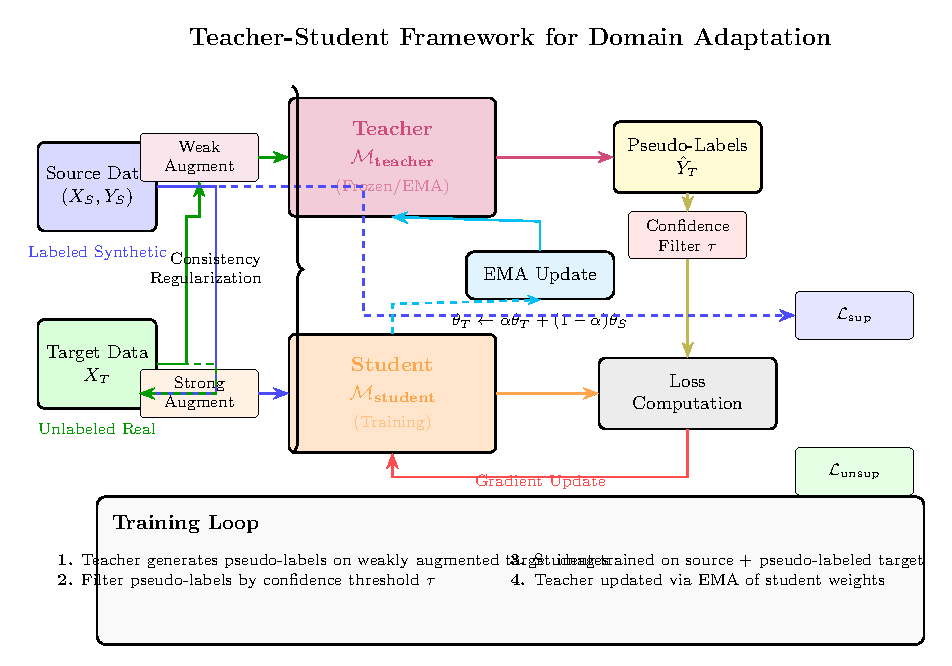
\includegraphics[width=\textwidth]{figures/ch06_fig4_teacher_student.pdf}
\caption{Teacher-student framework for domain adaptation in object detection. The teacher network generates pseudo-labels on weakly augmented target domain images, which are filtered by confidence threshold $\tau$. The student network is trained on both labeled source data (with supervised loss $\mathcal{L}_{\text{sup}}$) and pseudo-labeled target data (with unsupervised loss $\mathcal{L}_{\text{unsup}}$). Strong augmentation is applied to target images before student processing. The teacher weights are updated via exponential moving average (EMA) of student weights, providing stable pseudo-label generation throughout training.}
\label{fig:teacher_student}
\end{figure}

\begin{algorithm}[htbp]
\caption{Teacher-Student Domain Adaptation for Object Detection}
\label{alg:teacher_student}
\begin{algorithmic}[1]
\Require Labeled source data $\mathcal{D}_S = \{(x_S^i, y_S^i)\}$, unlabeled target data $\mathcal{D}_T = \{x_T^j\}$
\Require Pretrained source model $\mathcal{M}_S$, EMA decay rate $\alpha$
\Ensure Target-adapted student model $\mathcal{M}_{\text{student}}$
\State Initialize teacher $\mathcal{M}_{\text{teacher}} \leftarrow \mathcal{M}_S$
\State Initialize student $\mathcal{M}_{\text{student}} \leftarrow \mathcal{M}_S$
\For{epoch $= 1, 2, \ldots, E$}
    \For{each mini-batch $(x_S, y_S) \sim \mathcal{D}_S$, $x_T \sim \mathcal{D}_T$}
        \State \textbf{// Supervised loss on source data}
        \State $\mathcal{L}_{\text{sup}} \leftarrow \mathcal{L}_{\text{det}}(\mathcal{M}_{\text{student}}(x_S), y_S)$
        \State \textbf{// Generate pseudo-labels for target data}
        \State $\hat{y}_T \leftarrow \mathcal{M}_{\text{teacher}}(x_T)$
        \State Filter $\hat{y}_T$ by confidence threshold $\tau$
        \State \textbf{// Apply strong augmentation to target images}
        \State $\tilde{x}_T \leftarrow \text{StrongAugment}(x_T)$
        \State \textbf{// Unsupervised loss with pseudo-labels}
        \State $\mathcal{L}_{\text{unsup}} \leftarrow \mathcal{L}_{\text{det}}(\mathcal{M}_{\text{student}}(\tilde{x}_T), \hat{y}_T)$
        \State \textbf{// Combined loss and student update}
        \State $\mathcal{L} \leftarrow \mathcal{L}_{\text{sup}} + \lambda \mathcal{L}_{\text{unsup}}$
        \State Update $\mathcal{M}_{\text{student}}$ via gradient descent on $\mathcal{L}$
        \State \textbf{// Exponential moving average update for teacher}
        \State $\theta_{\text{teacher}} \leftarrow \alpha \theta_{\text{teacher}} + (1 - \alpha) \theta_{\text{student}}$
    \EndFor
\EndFor
\State \Return $\mathcal{M}_{\text{student}}$
\end{algorithmic}
\end{algorithm}

SF-YOLO represents a state-of-the-art instantiation of teacher-student adaptation for YOLO object detectors. The framework incorporates a Student Stabilization Module that prevents catastrophic forgetting of source domain knowledge during adaptation. Target-specific augmentations applied to student inputs but not teacher inputs encourage the student to develop robustness to target domain variations while maintaining consistency with teacher predictions.

The exponential moving average update for teacher weights provides temporal smoothing that stabilizes pseudo-label quality. The teacher represents an ensemble of student checkpoints weighted toward recent iterations, producing predictions that are more reliable than any single student checkpoint. The EMA decay rate $\alpha$ is typically set between 0.99 and 0.999, with higher values providing greater stability at the cost of slower adaptation to improved student representations.

\section{Measuring and Minimizing Domain Gap}
\label{sec:measuring_gap}

Effective domain adaptation requires methods for assessing the degree of distributional discrepancy and strategies for reducing identified gaps. This section presents approaches for domain gap measurement and gap-aware training methodologies.

\subsection{Domain Discriminator Approaches}

Training a discriminator network to classify features by domain origin provides both a measurement of domain gap and a mechanism for encouraging domain-invariant representations.

As a gap measurement tool, discriminator accuracy indicates the severity of distributional discrepancy. When source and target feature distributions are identical, no classifier can distinguish them better than random chance, yielding approximately fifty percent accuracy. As distributions diverge, discriminator accuracy increases toward perfect classification. The gap between observed accuracy and chance level quantifies the discriminability of domains in feature space.

\begin{figure}[htbp]
\centering
\begin{tikzpicture}[scale=0.85]
    % Feature space before alignment
    \begin{scope}[shift={(-5,0)}]
        \node[above] at (0,3) {\textbf{Before Alignment}};
        % Source cluster (synthetic)
        \draw[fill=blue!20, draw=blue] (-1.5,0) ellipse (1.2 and 1.5);
        \node[blue] at (-1.5,0) {$P_S$};
        % Target cluster (real)
        \draw[fill=red!20, draw=red] (1.5,0.5) ellipse (1.0 and 1.3);
        \node[red] at (1.5,0.5) {$P_T$};
        % Separating hyperplane
        \draw[thick, dashed, green!60!black] (0,-2) -- (0,2.5);
        \node[green!60!black, right] at (0.1,2) {\small Discriminator};
        \node[green!60!black, right] at (0.1,1.5) {\small boundary};
        % Scatter points
        \foreach \i in {1,...,15} {
            \pgfmathsetmacro{\x}{-1.5+0.8*rand}
            \pgfmathsetmacro{\y}{0.9*rand}
            \fill[blue] (\x,\y) circle (2pt);
        }
        \foreach \i in {1,...,12} {
            \pgfmathsetmacro{\x}{1.5+0.6*rand}
            \pgfmathsetmacro{\y}{0.5+0.8*rand}
            \fill[red] (\x,\y) circle (2pt);
        }
        \node[below] at (0,-2.5) {\small Acc. $\approx 95\%$};
    \end{scope}

    % Arrow
    \draw[->, ultra thick] (-1.5,0) -- (1.5,0);
    \node[above] at (0,0.3) {\small Domain};
    \node[below] at (0,-0.3) {\small Adaptation};

    % Feature space after alignment
    \begin{scope}[shift={(5,0)}]
        \node[above] at (0,3) {\textbf{After Alignment}};
        % Overlapping clusters
        \draw[fill=blue!20, draw=blue, opacity=0.5] (-0.3,0) ellipse (1.3 and 1.4);
        \draw[fill=red!20, draw=red, opacity=0.5] (0.3,0.1) ellipse (1.2 and 1.3);
        % Mixed scatter points
        \foreach \i in {1,...,15} {
            \pgfmathsetmacro{\x}{-0.3+0.9*rand}
            \pgfmathsetmacro{\y}{0.9*rand}
            \fill[blue] (\x,\y) circle (2pt);
        }
        \foreach \i in {1,...,12} {
            \pgfmathsetmacro{\x}{0.3+0.8*rand}
            \pgfmathsetmacro{\y}{0.1+0.8*rand}
            \fill[red] (\x,\y) circle (2pt);
        }
        \node[below] at (0,-2.5) {\small Acc. $\approx 55\%$};
    \end{scope}
\end{tikzpicture}
\caption{Domain shift in feature space before and after adaptation. High discriminator accuracy indicates substantial domain gap, while accuracy near chance level indicates well-aligned feature distributions.}
\label{fig:domain_shift}
\end{figure}

Multi-scale discriminators assess domain gap at different levels of feature abstraction. A discriminator operating on early layer features measures low-level appearance discrepancy arising from texture, color, and noise differences. Discriminators on deeper features assess higher-level semantic alignment. Jointly monitoring discriminators across scales provides a comprehensive picture of where domain gap manifests in the learned representation hierarchy.

Class-conditional discriminators separately assess domain gap for each object category. This granular analysis reveals which classes exhibit the largest synthetic-real discrepancy, enabling targeted improvement of synthetic data generation for problematic categories. Classes with high discriminator accuracy require additional variation in synthetic rendering to better match real-world appearance distributions.

\subsection{t-SNE Visualization Analysis}

Visual inspection of feature space structure through t-SNE projection provides intuitive understanding of domain relationships that complements quantitative metrics.

Joint embedding of synthetic and real features enables direct visual comparison of domain distributions. Features are extracted from both domains using the current model, concatenated, and jointly projected to two dimensions via t-SNE. The resulting visualization reveals whether synthetic and real features cluster separately or intermingle. Color-coding by domain origin and object class enables assessment of both domain-level and class-conditional alignment.

Temporal monitoring of t-SNE embeddings throughout training reveals the dynamics of domain adaptation. Initial projections typically show clear separation between synthetic and real clusters. As adaptation progresses, cluster overlap should increase, indicating that the model is learning domain-invariant representations. Failure of clusters to merge despite extended training suggests that the current adaptation approach is insufficient.

Class-specific analysis examines whether certain object categories exhibit greater domain gap than others. Even when overall distributions appear aligned, individual classes may remain separated, indicating that the model has achieved domain invariance for some categories while failing on others. This analysis guides prioritization of synthetic data improvement efforts.

\subsection{Automated Gap Estimation}

Manual inspection of visualizations and discriminator accuracies does not scale to continuous monitoring requirements of automated training systems. Automated gap estimation methods provide scalar metrics suitable for integration into training loops and optimization objectives.

Proxy A-distance provides a computationally efficient approximation to domain discrepancy. Given features from source and target domains, a linear classifier is trained to distinguish them, and the proxy A-distance is computed as $\hat{d}_A = 2(1 - 2\epsilon)$ where $\epsilon$ is the classifier error rate. This metric correlates with theoretical domain adaptation bounds and can be computed with minimal additional computation during training.

Feature distribution moments including mean, variance, and higher-order statistics provide simple gap indicators. The distance between domain-conditional feature means quantified by cosine similarity or Euclidean distance measures first-order distributional discrepancy. Matching variances addresses second-order differences. Maximum Mean Discrepancy provides a principled approach to comparing distributions through all moments via kernel embeddings.

Neural network-based gap estimators can be trained end-to-end to predict transfer performance from feature statistics. Given labeled transfer performance data from previous experiments, a regression network learns to map feature distribution summaries to expected target domain accuracy. Once trained, this predictor provides automated gap estimation for new synthetic data configurations without requiring full transfer evaluation.

\subsection{Gap-Aware Training Strategies}

Domain gap measurements can be integrated into training objectives to explicitly encourage gap minimization alongside task performance optimization.

Multi-objective optimization jointly minimizes task loss and domain discrepancy:
\begin{equation}
\mathcal{L}_{\text{total}} = \mathcal{L}_{\text{task}} + \lambda_{\text{gap}} \mathcal{L}_{\text{gap}}
\end{equation}
where $\mathcal{L}_{\text{task}}$ is the standard detection loss on labeled synthetic data and $\mathcal{L}_{\text{gap}}$ is a differentiable gap metric such as domain discriminator loss or MMD. The weighting parameter $\lambda_{\text{gap}}$ controls the relative importance of task performance versus domain alignment.

Curriculum-based gap reduction schedules the emphasis on gap minimization throughout training. Initial training phases focus primarily on task learning with minimal gap penalty. As task performance saturates, the gap penalty weight is increased to encourage continued domain adaptation. This curriculum prevents premature emphasis on gap reduction before the model has learned task-relevant features to align.

Adaptive weighting schemes adjust gap penalty importance based on current gap magnitude. When domain discrepancy is large, increased gap penalty accelerates alignment. When distributions are already well-aligned, reduced penalty avoids over-regularization that could harm task performance. This adaptive approach automatically balances task and domain objectives throughout training.

Gap-conditional data selection biases synthetic data sampling toward configurations that minimize domain gap. Synthetic images similar to real data under a learned gap metric are preferentially included in training batches. This approach focuses training computation on the most realistic synthetic examples rather than wasting resources on clearly out-of-distribution configurations.

\begin{table}[htbp]
\centering
\caption{Comparison of Domain Adaptation Methods for Object Detection}
\label{tab:da_methods}
\begin{tabular}{p{3cm}p{2.5cm}p{2.5cm}p{2.5cm}p{3cm}}
\toprule
\textbf{Method} & \textbf{Labeled Real Data} & \textbf{Unlabeled Real Data} & \textbf{Computational Cost} & \textbf{Typical Improvement} \\
\midrule
Fourier Domain Adaptation & Not required & Few samples & Very low & 3--8\% mAP \\
\addlinespace
Domain Discriminator & Not required & Recommended & Medium & 5--12\% mAP \\
\addlinespace
CycleGAN Style Transfer & Not required & Required & High & 4--10\% mAP \\
\addlinespace
Self-Training & Not required & Required & Medium & 8--15\% mAP \\
\addlinespace
Teacher-Student & Not required & Required & Medium-High & 10--18\% mAP \\
\addlinespace
Domain Randomization & Not required & Not required & Low & 15--25\% vs. no DR \\
\addlinespace
Fine-tuning on Real & Required & Optional & Low & 20--40\% mAP \\
\bottomrule
\end{tabular}
\end{table}

\section{Summary}

This chapter has provided a comprehensive treatment of domain adaptation and sim-to-real transfer for object detection systems. The domain gap problem arises from systematic differences between synthetic and real image distributions, manifesting in texture, lighting, sensor noise, and contextual composition discrepancies. Formal characterization of domain shift through distributional divergence metrics including FID, KID, and MMD enables quantitative assessment of synthetic data quality and guides optimization of data generation parameters.

Domain randomization provides a principled approach to sim-to-real transfer by training on sufficiently diverse synthetic distributions that encompass real-world conditions. Theoretical analysis establishes transfer bounds relating randomization breadth to expected generalization performance, revealing fundamental tradeoffs between exploration and robustness. Structured domain randomization improves upon uniform approaches by incorporating contextual constraints that focus generated examples on plausible configurations, achieving substantial gains in sample efficiency and transfer performance.

Active and adaptive domain randomization methods learn to optimize randomization parameters based on training feedback. Active Domain Randomization employs discriminative rewards to identify challenging environment configurations. DORAEMON formulates adaptive randomization as constrained entropy maximization, automatically constructing curricula from narrow to broad parameter distributions. These approaches provide principled mechanisms for the reinforcement learning-based optimization of synthetic data generation that motivates this textbook.

Domain adaptation techniques explicitly transform data or representations to reduce distributional discrepancy. Fourier Domain Adaptation transfers low-frequency appearance statistics from real to synthetic images through spectral manipulation. Adversarial feature alignment trains domain-invariant representations through gradient reversal. Teacher-student frameworks enable adaptation using unlabeled target domain data through pseudo-label generation and consistency regularization. The choice among these techniques depends on available data, computational resources, and target performance requirements.

Measuring and minimizing domain gap requires both quantitative metrics and visual analysis tools. Domain discriminator accuracy provides a learned measure of distributional discrepancy. t-SNE visualization enables intuitive assessment of feature space structure. Automated gap estimation methods scale to continuous monitoring requirements of automated training systems. Gap-aware training strategies integrate discrepancy minimization into optimization objectives, ensuring that learned representations achieve both task competence and domain invariance.

The techniques presented in this chapter form the foundation for autonomous optimization of synthetic data generation. By understanding the sources of domain gap, the mechanisms by which randomization enables transfer, and the methods available for measuring and minimizing discrepancy, practitioners can design reinforcement learning systems that automatically discover synthetic data configurations yielding robust real-world performance.


% Chapter 7: Reward Function Engineering
\chapter{Reward Function Engineering for Dataset Quality}
\label{ch:reward_functions}

The design of reward functions constitutes the most consequential architectural decision in any reinforcement learning system, and this principle applies with particular force to the optimization of synthetic data generation parameters for object detection. Unlike traditional reinforcement learning domains where reward signals emerge naturally from environmental dynamics, the synthetic data optimization context requires careful engineering of composite reward functions that integrate detection performance metrics, statistical reliability considerations, and auxiliary signals that promote beneficial exploration behavior. This chapter develops a comprehensive mathematical framework for reward function design, addressing the unique challenges posed by small validation sets, the risk of reward hacking, and the need to balance multiple competing objectives within a coherent optimization framework.

\section{Primary Reward Signals}
\label{sec:primary_reward}

The fundamental objective of synthetic data optimization is to discover generator configurations that produce training corpora yielding detectors with maximal performance on real-world imagery. This objective naturally suggests detection metrics computed on held-out real-world validation sets as the primary reward signal. However, the translation of this intuition into mathematically rigorous reward formulations requires careful consideration of metric properties, aggregation strategies, and the relationship between component metrics and overall detection quality.

\subsection{Mean Average Precision as the Primary Objective}

Mean Average Precision (mAP) has emerged as the predominant evaluation metric for object detection systems, serving as the primary benchmark in competitions such as PASCAL VOC and MS COCO. The metric integrates precision-recall trade-offs across detection thresholds and object classes, providing a comprehensive assessment of detector quality that aligns well with practical deployment requirements.

For a detector producing predictions on a validation set containing ground truth annotations across $C$ object classes, the computation of mAP proceeds through several stages. Let $\mathcal{D} = \{(x_i, \mathcal{Y}_i)\}_{i=1}^{N}$ denote the validation set comprising $N$ images, where each $\mathcal{Y}_i = \{(b_j, c_j)\}_{j=1}^{M_i}$ contains $M_i$ ground truth bounding boxes $b_j \in \mathbb{R}^4$ with associated class labels $c_j \in \{1, \ldots, C\}$. The detector produces predictions $\hat{\mathcal{Y}}_i = \{(\hat{b}_k, \hat{c}_k, \hat{s}_k)\}_{k=1}^{\hat{M}_i}$ where $\hat{s}_k \in [0, 1]$ denotes the confidence score associated with each detection.

The Intersection over Union (IoU) between a predicted bounding box $\hat{b} = (\hat{x}_1, \hat{y}_1, \hat{x}_2, \hat{y}_2)$ and a ground truth box $b = (x_1, y_1, x_2, y_2)$ is computed as:
\begin{equation}
\text{IoU}(\hat{b}, b) = \frac{|\hat{b} \cap b|}{|\hat{b} \cup b|} = \frac{\text{Area}(\hat{b} \cap b)}{\text{Area}(\hat{b}) + \text{Area}(b) - \text{Area}(\hat{b} \cap b)}
\label{eq:iou_definition}
\end{equation}
where the intersection area is computed as:
\begin{equation}
\text{Area}(\hat{b} \cap b) = \max(0, \min(\hat{x}_2, x_2) - \max(\hat{x}_1, x_1)) \cdot \max(0, \min(\hat{y}_2, y_2) - \max(\hat{y}_1, y_1))
\end{equation}

A detection is classified as a true positive for class $c$ at IoU threshold $\tau$ if there exists a ground truth box $b$ of the same class such that $\text{IoU}(\hat{b}, b) \geq \tau$ and neither the prediction nor the ground truth has been previously matched. The matching proceeds in order of decreasing confidence scores $\hat{s}_k$, ensuring that higher-confidence predictions receive priority in the matching process.

Let $\text{TP}_c(\tau, t)$ and $\text{FP}_c(\tau, t)$ denote the cumulative true positive and false positive counts for class $c$ at IoU threshold $\tau$ when considering all predictions with confidence scores exceeding threshold $t$. The precision and recall at this operating point are:
\begin{equation}
P_c(\tau, t) = \frac{\text{TP}_c(\tau, t)}{\text{TP}_c(\tau, t) + \text{FP}_c(\tau, t)}, \quad R_c(\tau, t) = \frac{\text{TP}_c(\tau, t)}{|\mathcal{G}_c|}
\label{eq:precision_recall}
\end{equation}
where $|\mathcal{G}_c|$ denotes the total number of ground truth objects of class $c$ across the validation set.

The precision-recall curve for class $c$ at IoU threshold $\tau$ is obtained by varying the confidence threshold $t$ and computing the corresponding precision-recall pairs. The Average Precision (AP) for class $c$ is computed as the area under this curve:
\begin{equation}
\text{AP}_c(\tau) = \int_0^1 P_c(\tau, R) \, dR \approx \sum_{k=1}^{K} (R_k - R_{k-1}) \cdot P_{\text{interp}}(R_k)
\label{eq:average_precision}
\end{equation}
where $P_{\text{interp}}(R_k) = \max_{R' \geq R_k} P(R')$ represents the interpolated precision at recall level $R_k$, following the eleven-point or all-point interpolation schemes employed in standard benchmarks.

The mean Average Precision across all classes is then:
\begin{equation}
\text{mAP}(\tau) = \frac{1}{C} \sum_{c=1}^{C} \text{AP}_c(\tau)
\label{eq:map_single_threshold}
\end{equation}

The COCO-style mAP extends this computation by averaging across multiple IoU thresholds:
\begin{equation}
\text{mAP}_{\text{COCO}} = \frac{1}{|\mathcal{T}|} \sum_{\tau \in \mathcal{T}} \text{mAP}(\tau)
\label{eq:map_coco}
\end{equation}
where $\mathcal{T} = \{0.50, 0.55, \ldots, 0.95\}$ comprises ten IoU thresholds spanning from lenient to stringent matching criteria.

\begin{figure}[t]
\centering
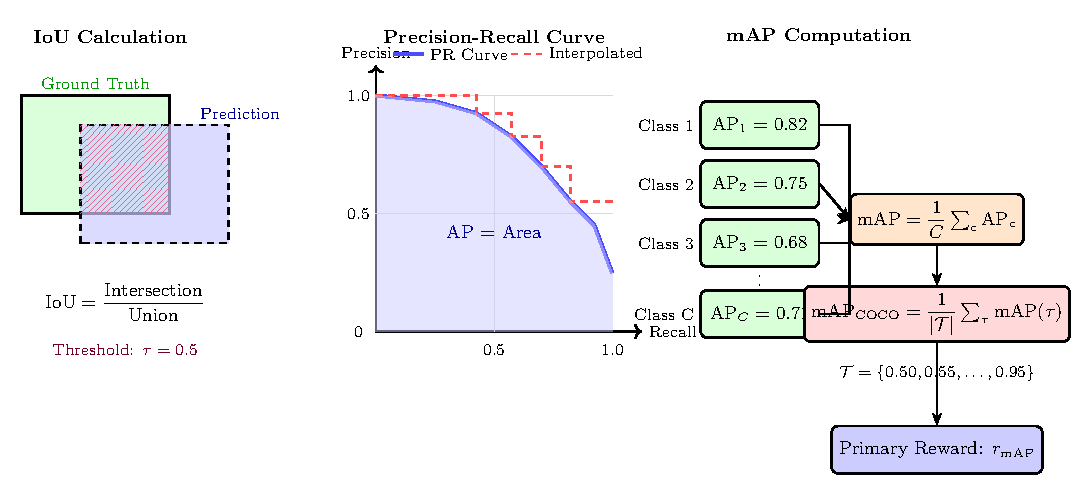
\includegraphics[width=\textwidth]{figures/ch07_fig1_map_calculation.pdf}
\caption{Visualization of mAP computation showing three key stages: (left) IoU calculation between predicted and ground truth bounding boxes with the intersection highlighted, (center) precision-recall curve with the shaded area representing Average Precision, and (right) aggregation of per-class AP values into mAP and the COCO-style averaging across multiple IoU thresholds.}
\label{fig:map_calculation}
\end{figure}

The primary reward signal based on mAP is thus defined as:
\begin{equation}
r_{\text{mAP}} = \text{mAP}_{\text{COCO}}(\theta) = \text{mAP}(\mathcal{D}_{\text{val}}, f_{\phi(\theta)})
\label{eq:reward_map}
\end{equation}
where $\theta$ denotes the synthetic data generator parameters, $\phi(\theta)$ represents the detector weights obtained by training on synthetic data generated with parameters $\theta$, and $f_{\phi(\theta)}$ denotes the resulting detector.

\subsection{Component Metrics and Their Relationships}

While mAP serves as the primary optimization objective, understanding the component metrics provides valuable diagnostic information and enables the construction of more nuanced reward signals. The decomposition of detection performance into precision, recall, and localization quality reveals distinct failure modes that may require targeted intervention through auxiliary reward components.

Precision measures the fraction of detector predictions that correspond to actual objects, quantifying the rate of false positive errors. High precision is essential in applications where false alarms carry significant costs, such as autonomous driving scenarios where phantom detections might trigger unnecessary emergency maneuvers. The precision at a fixed confidence threshold $t^*$ is given by:
\begin{equation}
\text{Precision}(t^*) = \frac{\sum_{c=1}^{C} \text{TP}_c(\tau, t^*)}{\sum_{c=1}^{C} (\text{TP}_c(\tau, t^*) + \text{FP}_c(\tau, t^*))}
\label{eq:precision_fixed}
\end{equation}

Recall measures the fraction of ground truth objects successfully detected, quantifying the rate of false negative errors. High recall is critical in applications where missed detections carry severe consequences, such as medical imaging where overlooked abnormalities might delay life-saving treatment. The recall at confidence threshold $t^*$ is:
\begin{equation}
\text{Recall}(t^*) = \frac{\sum_{c=1}^{C} \text{TP}_c(\tau, t^*)}{\sum_{c=1}^{C} |\mathcal{G}_c|}
\label{eq:recall_fixed}
\end{equation}

The F1 score provides a harmonic mean of precision and recall, offering a single metric that penalizes extreme imbalances between the two:
\begin{equation}
F_1 = \frac{2 \cdot \text{Precision} \cdot \text{Recall}}{\text{Precision} + \text{Recall}} = \frac{2 \cdot \text{TP}}{2 \cdot \text{TP} + \text{FP} + \text{FN}}
\label{eq:f1_score}
\end{equation}

Localization quality, as captured by the IoU distribution of matched detections, provides insight into the geometric accuracy of bounding box predictions. The mean IoU of true positive detections is:
\begin{equation}
\overline{\text{IoU}} = \frac{1}{|\text{TP}|} \sum_{(\hat{b}, b) \in \text{TP}} \text{IoU}(\hat{b}, b)
\label{eq:mean_iou}
\end{equation}

\subsection{Class-Specific versus Aggregate Rewards}

The aggregation strategy employed when combining per-class metrics into a scalar reward has significant implications for optimization dynamics, particularly when class frequencies are imbalanced or when different classes exhibit varying difficulty levels.

The standard mAP formulation employs uniform weighting across classes, treating all classes as equally important regardless of their frequency in the validation set:
\begin{equation}
r_{\text{uniform}} = \frac{1}{C} \sum_{c=1}^{C} \text{AP}_c
\label{eq:uniform_weighting}
\end{equation}

Frequency-weighted aggregation assigns weights proportional to class prevalence, emphasizing performance on common classes:
\begin{equation}
r_{\text{freq}} = \sum_{c=1}^{C} \frac{|\mathcal{G}_c|}{\sum_{c'} |\mathcal{G}_{c'}|} \cdot \text{AP}_c
\label{eq:frequency_weighting}
\end{equation}

Inverse-frequency weighting places greater emphasis on rare classes, which may be appropriate when rare classes carry particular practical importance:
\begin{equation}
r_{\text{inv-freq}} = \sum_{c=1}^{C} \frac{1/|\mathcal{G}_c|}{\sum_{c'} 1/|\mathcal{G}_{c'}|} \cdot \text{AP}_c
\label{eq:inverse_frequency_weighting}
\end{equation}

Worst-case class performance provides a max-min objective that prevents the optimizer from sacrificing performance on difficult classes:
\begin{equation}
r_{\text{worst}} = \min_{c \in \{1, \ldots, C\}} \text{AP}_c
\label{eq:worst_case}
\end{equation}

A hybrid formulation that balances average performance with worst-case guarantees employs a convex combination:
\begin{equation}
r_{\text{hybrid}} = (1 - \lambda) \cdot \text{mAP} + \lambda \cdot \min_c \text{AP}_c
\label{eq:hybrid_aggregation}
\end{equation}
where $\lambda \in [0, 1]$ controls the trade-off between average and worst-case optimization.

\subsection{Confidence-Weighted Metrics}

The confidence scores produced by modern object detectors provide valuable information about prediction reliability that can be incorporated into reward formulations. Confidence-weighted metrics encourage the detector to produce well-calibrated predictions where confidence scores accurately reflect detection accuracy.

The Expected Calibration Error (ECE) measures the discrepancy between predicted confidence and empirical accuracy:
\begin{equation}
\text{ECE} = \sum_{m=1}^{M} \frac{|B_m|}{N} \left| \text{acc}(B_m) - \text{conf}(B_m) \right|
\label{eq:ece}
\end{equation}
where predictions are partitioned into $M$ bins $\{B_m\}$ based on confidence scores, $\text{acc}(B_m)$ denotes the fraction of predictions in bin $B_m$ that are true positives, and $\text{conf}(B_m)$ denotes the average confidence in the bin.

A reward term penalizing miscalibration can be incorporated as:
\begin{equation}
r_{\text{calibration}} = 1 - \text{ECE}
\label{eq:calibration_reward}
\end{equation}

Confidence-weighted precision assigns greater importance to high-confidence predictions:
\begin{equation}
\text{Precision}_{\text{conf}} = \frac{\sum_k \hat{s}_k \cdot \mathbb{1}[\text{TP}_k]}{\sum_k \hat{s}_k}
\label{eq:confidence_weighted_precision}
\end{equation}
where $\mathbb{1}[\text{TP}_k]$ indicates whether prediction $k$ is a true positive.

\section{Handling Small Validation Sets}
\label{sec:small_validation}

The practical constraints of many synthetic data optimization scenarios necessitate validation against severely limited real-world imagery, often comprising fewer than one hundred annotated frames. This limitation introduces substantial statistical challenges, as performance estimates computed on small samples exhibit high variance and may not reliably indicate true detector quality. This section develops mathematical frameworks for addressing these challenges through bootstrap confidence estimation, cross-validation strategies, and variance reduction techniques.

\subsection{Statistical Challenges with Limited Samples}

Consider the task of estimating mAP from a validation set containing $N = 50$ images. The standard error of the mAP estimate depends on the underlying variance of per-image performance and can be approximated as:
\begin{equation}
\text{SE}(\widehat{\text{mAP}}) \approx \frac{\sigma_{\text{mAP}}}{\sqrt{N}}
\label{eq:standard_error}
\end{equation}
where $\sigma_{\text{mAP}}$ represents the standard deviation of per-image AP contributions.

For typical object detection scenarios where $\sigma_{\text{mAP}} \approx 0.15$, a validation set of 50 images yields a standard error of approximately 0.02, implying that 95\% confidence intervals span roughly $\pm 0.04$ mAP points. This level of uncertainty is substantial relative to the performance improvements typically sought through synthetic data optimization, which may target gains of 0.05 to 0.10 mAP points.

The challenge is compounded by the non-uniform distribution of objects across images. Let $n_i$ denote the number of ground truth objects in image $i$. The effective sample size for estimating class-specific AP depends on the total object count rather than the image count:
\begin{equation}
N_{\text{eff},c} = \sum_{i=1}^{N} n_{i,c}
\label{eq:effective_sample_size}
\end{equation}
where $n_{i,c}$ counts objects of class $c$ in image $i$. For rare classes with $N_{\text{eff},c} < 20$, AP estimates become highly unreliable.

\subsection{Bootstrap Confidence Intervals}

Bootstrap resampling provides a non-parametric approach to estimating the sampling distribution of mAP and constructing confidence intervals that account for the complex dependence structure of detection metrics. The procedure involves repeatedly resampling the validation set with replacement and computing mAP on each bootstrap sample.

\begin{algorithm}[t]
\caption{Bootstrap Confidence Interval for mAP}
\label{alg:bootstrap_confidence}
\begin{algorithmic}[1]
\Require Validation set $\mathcal{D} = \{(x_i, \mathcal{Y}_i)\}_{i=1}^{N}$, detector $f$, number of bootstrap samples $B$, confidence level $1 - \alpha$
\Ensure Point estimate $\widehat{\text{mAP}}$, confidence interval $[\text{mAP}_{\text{lo}}, \text{mAP}_{\text{hi}}]$
\State Compute point estimate $\widehat{\text{mAP}} \gets \text{mAP}(\mathcal{D}, f)$
\For{$b = 1$ to $B$}
    \State Sample indices $\mathcal{I}^{(b)} \gets \{i_1^{(b)}, \ldots, i_N^{(b)}\}$ uniformly with replacement from $\{1, \ldots, N\}$
    \State Construct bootstrap sample $\mathcal{D}^{(b)} \gets \{(x_{i_j^{(b)}}, \mathcal{Y}_{i_j^{(b)}})\}_{j=1}^{N}$
    \State Compute bootstrap estimate $\text{mAP}^{(b)} \gets \text{mAP}(\mathcal{D}^{(b)}, f)$
\EndFor
\State Compute bootstrap standard error $\hat{\sigma}_{\text{boot}} \gets \sqrt{\frac{1}{B-1} \sum_{b=1}^{B} (\text{mAP}^{(b)} - \bar{\text{mAP}})^2}$
\State Sort bootstrap estimates: $\text{mAP}^{(1)} \leq \text{mAP}^{(2)} \leq \cdots \leq \text{mAP}^{(B)}$
\State \textbf{Percentile method:} $\text{mAP}_{\text{lo}} \gets \text{mAP}^{(\lfloor B \cdot \alpha/2 \rfloor)}$, $\text{mAP}_{\text{hi}} \gets \text{mAP}^{(\lceil B \cdot (1-\alpha/2) \rceil)}$
\State \textbf{BCa correction (optional):} Apply bias-correction and acceleration adjustments
\State \Return $\widehat{\text{mAP}}$, $[\text{mAP}_{\text{lo}}, \text{mAP}_{\text{hi}}]$
\end{algorithmic}
\end{algorithm}

The percentile bootstrap confidence interval is obtained by taking the $\alpha/2$ and $1 - \alpha/2$ quantiles of the bootstrap distribution. For a 95\% confidence interval with $B = 1000$ bootstrap samples, this corresponds to the 25th and 975th order statistics.

The bias-corrected and accelerated (BCa) bootstrap provides improved coverage properties by adjusting for bias and skewness in the bootstrap distribution:
\begin{equation}
\text{mAP}_{\text{lo}}^{\text{BCa}} = \hat{G}^{-1}\left( \Phi\left( \hat{z}_0 + \frac{\hat{z}_0 + z_{\alpha/2}}{1 - \hat{a}(\hat{z}_0 + z_{\alpha/2})} \right) \right)
\label{eq:bca_lower}
\end{equation}
where $\hat{G}$ denotes the empirical CDF of bootstrap estimates, $\Phi$ is the standard normal CDF, $z_{\alpha/2} = \Phi^{-1}(\alpha/2)$, and the bias-correction factor $\hat{z}_0$ and acceleration factor $\hat{a}$ are computed from the bootstrap distribution and jackknife influence values, respectively.

The bias-correction factor is estimated as:
\begin{equation}
\hat{z}_0 = \Phi^{-1}\left( \frac{1}{B} \sum_{b=1}^{B} \mathbb{1}[\text{mAP}^{(b)} < \widehat{\text{mAP}}] \right)
\label{eq:bias_correction}
\end{equation}

The acceleration factor is computed using jackknife resampling:
\begin{equation}
\hat{a} = \frac{\sum_{i=1}^{N} (\bar{\theta}_{(\cdot)} - \hat{\theta}_{(-i)})^3}{6 \left( \sum_{i=1}^{N} (\bar{\theta}_{(\cdot)} - \hat{\theta}_{(-i)})^2 \right)^{3/2}}
\label{eq:acceleration_factor}
\end{equation}
where $\hat{\theta}_{(-i)}$ denotes the mAP estimate with the $i$-th image removed and $\bar{\theta}_{(\cdot)} = \frac{1}{N} \sum_i \hat{\theta}_{(-i)}$.

\subsection{Cross-Validation Strategies}

Cross-validation provides an alternative approach to variance reduction that partitions the validation set into complementary subsets, enabling more robust performance estimation through averaging across multiple evaluation folds.

$K$-fold cross-validation partitions the validation set into $K$ disjoint subsets $\{\mathcal{D}_1, \ldots, \mathcal{D}_K\}$ and computes performance on each fold:
\begin{equation}
\widehat{\text{mAP}}_{\text{CV}} = \frac{1}{K} \sum_{k=1}^{K} \text{mAP}(\mathcal{D}_k, f)
\label{eq:cv_estimate}
\end{equation}

The variance of the cross-validation estimate can be approximated as:
\begin{equation}
\text{Var}(\widehat{\text{mAP}}_{\text{CV}}) \approx \frac{\sigma^2_{\text{fold}}}{K} + \frac{K-1}{K} \rho \sigma^2_{\text{fold}}
\label{eq:cv_variance}
\end{equation}
where $\sigma^2_{\text{fold}}$ is the variance of per-fold estimates and $\rho$ is the correlation between estimates computed on different folds. The second term reflects the positive correlation induced by shared training data (when cross-validation is applied to the training procedure) or shared model parameters (when applied only to evaluation).

Stratified cross-validation ensures that each fold maintains approximately the same class distribution as the full validation set, which is particularly important when class frequencies are imbalanced:
\begin{equation}
\frac{|\mathcal{G}_{c,k}|}{|\mathcal{D}_k|} \approx \frac{|\mathcal{G}_c|}{|\mathcal{D}|} \quad \forall c, k
\label{eq:stratified_cv}
\end{equation}

Repeated cross-validation performs multiple rounds of $K$-fold cross-validation with different random partitions, further reducing variance at the cost of increased computation:
\begin{equation}
\widehat{\text{mAP}}_{\text{RCV}} = \frac{1}{R \cdot K} \sum_{r=1}^{R} \sum_{k=1}^{K} \text{mAP}(\mathcal{D}_{r,k}, f)
\label{eq:repeated_cv}
\end{equation}

\subsection{Variance Reduction Techniques}

Beyond bootstrap and cross-validation, several additional techniques can reduce the variance of reward estimates, improving the signal-to-noise ratio available to the reinforcement learning optimizer.

Control variates exploit correlation with auxiliary variables whose expectations are known. Let $Y = \text{mAP}$ be the quantity of interest and $X$ be a correlated auxiliary variable. The control variate estimator is:
\begin{equation}
\hat{Y}_{\text{CV}} = Y - \beta(X - \mathbb{E}[X])
\label{eq:control_variate}
\end{equation}
where $\beta^* = \text{Cov}(Y, X) / \text{Var}(X)$ minimizes variance. In the synthetic data context, $X$ might represent performance on a larger synthetic validation set, with $\mathbb{E}[X]$ estimated from historical data.

Antithetic variates reduce variance by introducing negative correlation between paired samples. When evaluating multiple generator configurations, antithetic sampling ensures that high-variance images appear in complementary positions across evaluations, inducing negative covariance that reduces the variance of performance differences.

Common random numbers use the same random seed for stochastic elements (such as data augmentation during evaluation) across different generator configurations, ensuring that performance differences reflect true configuration effects rather than random variation:
\begin{equation}
\text{Var}(\hat{Y}_1 - \hat{Y}_2) = \text{Var}(\hat{Y}_1) + \text{Var}(\hat{Y}_2) - 2\text{Cov}(\hat{Y}_1, \hat{Y}_2)
\label{eq:common_random_numbers}
\end{equation}

When evaluations share random elements, $\text{Cov}(\hat{Y}_1, \hat{Y}_2) > 0$, reducing the variance of the difference.

\subsection{Conservative Reward Estimation}

Given the high variance of performance estimates on small validation sets, conservative reward estimation provides a principled approach to avoiding over-optimistic evaluations that might lead to poor generalization. Rather than using the point estimate $\widehat{\text{mAP}}$, conservative approaches employ lower confidence bounds:
\begin{equation}
r_{\text{conservative}} = \widehat{\text{mAP}} - \kappa \cdot \hat{\sigma}_{\text{boot}}
\label{eq:conservative_reward}
\end{equation}
where $\kappa > 0$ controls the degree of conservatism. Setting $\kappa = 1.96$ corresponds to using the lower bound of a 95\% confidence interval.

The lower confidence bound (LCB) approach is analogous to acquisition functions in Bayesian optimization and implements a form of pessimism under uncertainty that has theoretical justification in the bandit literature. By penalizing high-variance configurations, LCB encourages exploration of regions where performance estimates are reliable.

\section{Reward Shaping Strategies}
\label{sec:reward_shaping}

Pure reliance on the terminal mAP signal presents several challenges for reinforcement learning optimization. The reward is sparse, available only after complete detector training cycles that may require hours of computation. The signal is noisy due to small validation set sizes. And the reward provides limited guidance about the direction of improvement, offering only a scalar summary of detector quality without indicating which aspects of synthetic data generation require modification. Reward shaping addresses these limitations by introducing intermediate signals that guide learning while preserving the optimality of policies that maximize the original objective.

\subsection{Intermediate Rewards During Training}

The detector training process generates a rich stream of intermediate signals that can inform reward computation without waiting for final convergence. Training loss curves, validation performance trajectories, and convergence dynamics all provide information about the quality of synthetic data that can be incorporated into shaped reward functions.

The training loss at epoch $e$ when training on synthetic data generated with parameters $\theta$ is denoted $\mathcal{L}_{\text{train}}(e; \theta)$. The rate of loss decrease provides a signal about learning efficiency:
\begin{equation}
\Delta \mathcal{L}(e; \theta) = \mathcal{L}_{\text{train}}(e-1; \theta) - \mathcal{L}_{\text{train}}(e; \theta)
\label{eq:loss_decrease}
\end{equation}

Configurations yielding faster initial loss decrease often indicate better alignment between synthetic and real data distributions, as the detector can more readily extract transferable features.

An intermediate reward based on early training dynamics is:
\begin{equation}
r_{\text{early}}(\theta) = \frac{1}{E_{\text{early}}} \sum_{e=1}^{E_{\text{early}}} \Delta \mathcal{L}(e; \theta)
\label{eq:early_training_reward}
\end{equation}
where $E_{\text{early}} \ll E_{\text{total}}$ represents an early checkpoint (e.g., 10\% of total training epochs).

The validation loss trajectory provides complementary information about generalization:
\begin{equation}
r_{\text{val-trajectory}}(\theta) = -\min_{e \leq E_{\text{total}}} \mathcal{L}_{\text{val}}(e; \theta)
\label{eq:val_trajectory_reward}
\end{equation}

\subsection{Loss-Based Progress Signals}

The components of the YOLO loss function provide granular feedback about different aspects of detector learning. The total loss decomposes as:
\begin{equation}
\mathcal{L}_{\text{YOLO}} = \lambda_{\text{box}} \mathcal{L}_{\text{box}} + \lambda_{\text{obj}} \mathcal{L}_{\text{obj}} + \lambda_{\text{cls}} \mathcal{L}_{\text{cls}}
\label{eq:yolo_loss_decomposition}
\end{equation}
where $\mathcal{L}_{\text{box}}$ measures localization accuracy, $\mathcal{L}_{\text{obj}}$ measures objectness prediction quality, and $\mathcal{L}_{\text{cls}}$ measures classification accuracy.

Modern YOLO variants employ CIoU (Complete Intersection over Union) loss for bounding box regression:
\begin{equation}
\mathcal{L}_{\text{CIoU}} = 1 - \text{IoU} + \frac{\rho^2(b, b^{\text{gt}})}{c^2} + \alpha v
\label{eq:ciou_loss}
\end{equation}
where $\rho(b, b^{\text{gt}})$ is the Euclidean distance between box centers, $c$ is the diagonal length of the smallest enclosing box, $v = \frac{4}{\pi^2}(\arctan(w^{\text{gt}}/h^{\text{gt}}) - \arctan(w/h))^2$ measures aspect ratio consistency, and $\alpha = v / ((1 - \text{IoU}) + v)$.

Monitoring the convergence of individual loss components enables diagnosis of synthetic data deficiencies. Slow convergence of $\mathcal{L}_{\text{box}}$ may indicate unrealistic object scales or positions in synthetic data. Poor $\mathcal{L}_{\text{cls}}$ convergence suggests insufficient class-discriminative features. Elevated $\mathcal{L}_{\text{obj}}$ points to background characteristics that differ between synthetic and real domains.

\subsection{Curriculum-Based Reward Schedules}

Curriculum-based reward schedules modify the reward function over the course of optimization, typically progressing from lenient to stringent evaluation criteria. This approach mirrors the curriculum learning paradigm in supervised learning, where models are trained on progressively more difficult examples.

A time-varying IoU threshold schedule for mAP computation is:
\begin{equation}
\tau(t) = \tau_{\text{min}} + (\tau_{\text{max}} - \tau_{\text{min}}) \cdot \sigma\left(\frac{t - t_0}{T}\right)
\label{eq:curriculum_iou}
\end{equation}
where $\sigma(\cdot)$ is a sigmoid function providing smooth interpolation, $t$ is the optimization iteration, and $T$ controls the transition rate. Early iterations use lenient thresholds ($\tau_{\text{min}} = 0.3$) that reward approximate detections, while later iterations require precise localization ($\tau_{\text{max}} = 0.75$).

Curriculum weighting of mAP components follows a similar principle:
\begin{equation}
r_{\text{curriculum}}(t) = w_{\text{det}}(t) \cdot \text{mAP}_{50} + w_{\text{loc}}(t) \cdot \text{mAP}_{75} + w_{\text{strict}}(t) \cdot \text{mAP}_{50:95}
\label{eq:curriculum_weighting}
\end{equation}
where the weights evolve from detection-focused ($w_{\text{det}} \gg w_{\text{strict}}$) to localization-focused ($w_{\text{strict}} \gg w_{\text{det}}$) as optimization progresses.

\begin{figure}[t]
\centering
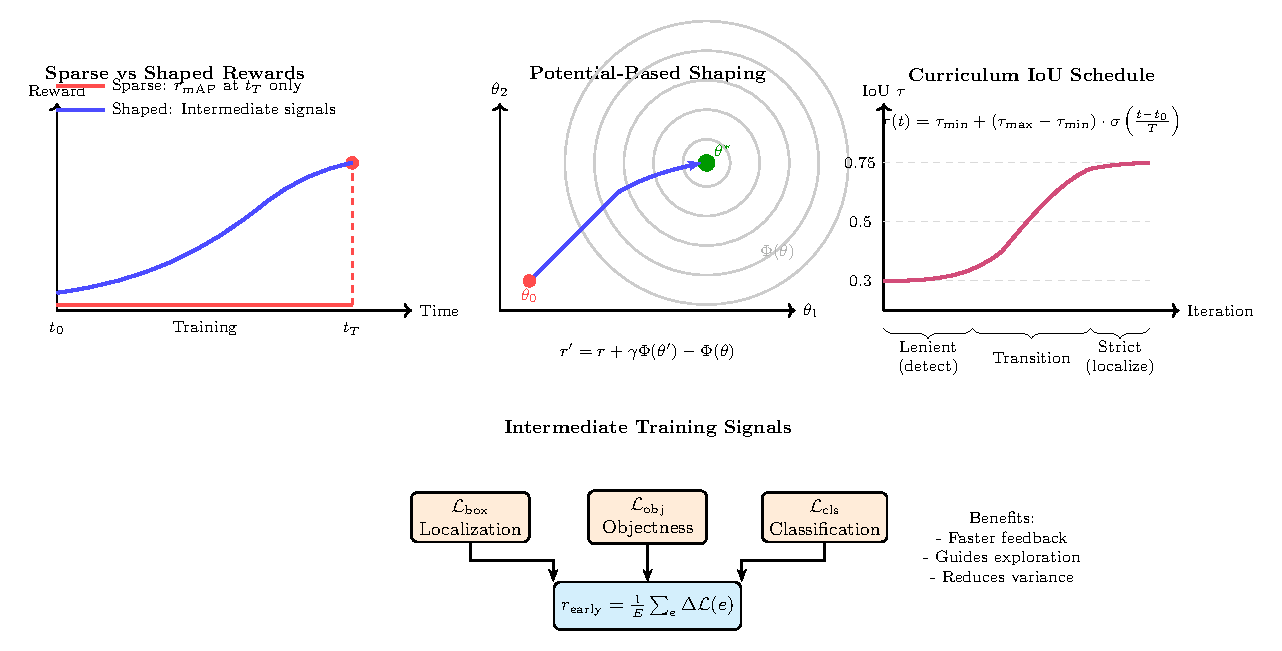
\includegraphics[width=\textwidth]{figures/ch07_fig2_reward_shaping.pdf}
\caption{Reward shaping strategies for synthetic data optimization. Top left: Comparison of sparse rewards (available only at training completion) versus shaped rewards (providing continuous feedback). Top center: Potential-based shaping guiding optimization toward known good configurations $\theta^*$. Top right: Curriculum IoU schedule transitioning from lenient detection thresholds to strict localization requirements. Bottom: Integration of intermediate training signals from YOLO loss components to provide early feedback.}
\label{fig:reward_shaping}
\end{figure}

\subsection{Multi-Objective Reward Balancing}

Synthetic data optimization involves multiple competing objectives: detection accuracy, computational efficiency, diversity, and domain alignment. Multi-objective reward balancing combines these signals into a coherent scalar reward while preserving sensitivity to each component.

Linear scalarization combines objectives with fixed weights:
\begin{equation}
r_{\text{linear}} = \sum_{i=1}^{M} w_i \cdot r_i
\label{eq:linear_scalarization}
\end{equation}

The choice of weights $\{w_i\}$ determines which points on the Pareto frontier are achievable through optimization. Different weight vectors trace out different regions of the frontier, but convex combinations cannot reach non-convex regions.

Chebyshev scalarization addresses this limitation by minimizing the maximum weighted deviation from an ideal point:
\begin{equation}
r_{\text{Chebyshev}} = -\max_{i \in \{1, \ldots, M\}} w_i \cdot |r_i^* - r_i|
\label{eq:chebyshev_scalarization}
\end{equation}
where $r_i^*$ represents the ideal (maximum achievable) value for objective $i$.

Achievement scalarizing functions generalize these approaches:
\begin{equation}
r_{\text{ASF}} = \min_{i} \frac{r_i - r_i^{\text{ref}}}{r_i^* - r_i^{\text{ref}}} + \rho \sum_{i} \frac{r_i - r_i^{\text{ref}}}{r_i^* - r_i^{\text{ref}}}
\label{eq:asf}
\end{equation}
where $r_i^{\text{ref}}$ is a reference point and $\rho > 0$ is a small constant ensuring strict monotonicity.

\begin{figure}[t]
\centering
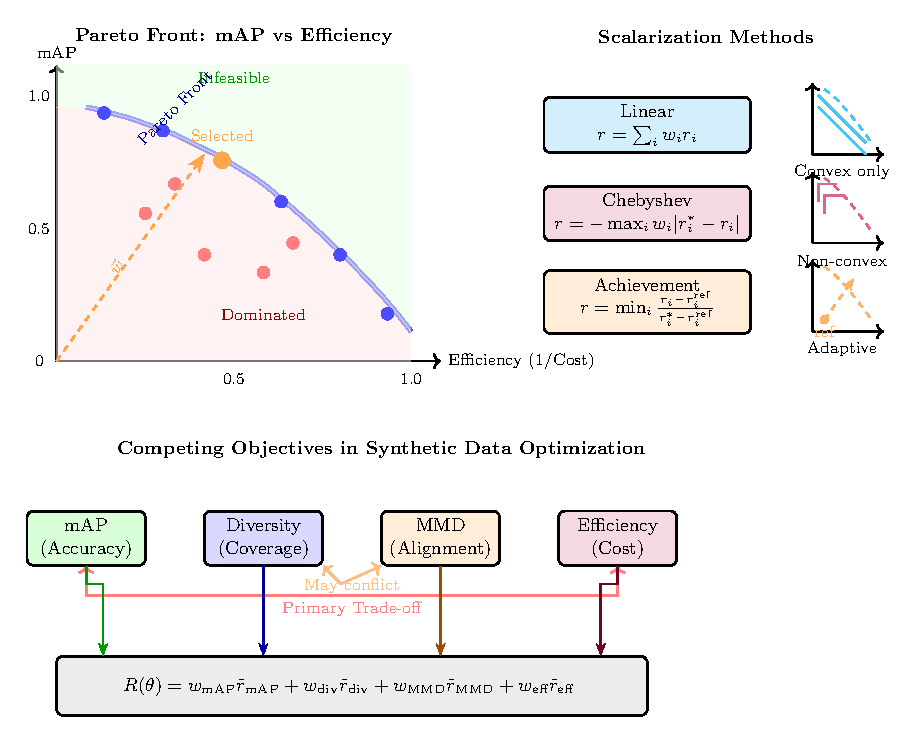
\includegraphics[width=\textwidth]{figures/ch07_fig3_pareto_front.pdf}
\caption{Multi-objective optimization in reward function design. Left: Pareto front illustrating the trade-off between mAP (accuracy) and efficiency, with dominated solutions shown in the shaded region and Pareto-optimal configurations on the frontier. A weight vector $\vec{w}$ determines which point on the frontier is selected. Right: Three scalarization methods (linear, Chebyshev, and achievement functions) with their geometric interpretations. Bottom: The competing objectives in synthetic data optimization and how they combine into the composite reward function.}
\label{fig:pareto_front}
\end{figure}

\subsection{Potential-Based Reward Shaping Theory}

The theoretical foundation for reward shaping rests on the concept of potential-based shaping, which guarantees that shaped rewards preserve optimal policies. Let $\Phi: \mathcal{S} \to \mathbb{R}$ be a potential function defined over states. The shaped reward is:
\begin{equation}
r'(s, a, s') = r(s, a, s') + \gamma \Phi(s') - \Phi(s)
\label{eq:potential_based_shaping}
\end{equation}
where $\gamma$ is the discount factor. This formulation ensures that policies optimal under $r'$ are also optimal under $r$, as the potential terms telescope when computing cumulative returns.

In the synthetic data optimization context, the state space consists of generator configurations $\theta$, and a natural potential function measures proximity to known good configurations:
\begin{equation}
\Phi(\theta) = \max_{\theta^* \in \Theta_{\text{good}}} \exp\left( -\frac{\|\theta - \theta^*\|^2}{2\sigma^2} \right)
\label{eq:configuration_potential}
\end{equation}
where $\Theta_{\text{good}}$ contains historically successful configurations.

The shaped reward encourages movement toward promising regions of the configuration space while preserving the global optimum defined by mAP:
\begin{equation}
r'(\theta, \theta') = r_{\text{mAP}}(\theta') + \gamma \Phi(\theta') - \Phi(\theta)
\label{eq:shaped_reward_synthetic}
\end{equation}

\section{Auxiliary Reward Components}
\label{sec:auxiliary_rewards}

Beyond the primary detection performance signal, auxiliary reward components address failure modes and desiderata that are not captured by mAP alone. These components include diversity bonuses that prevent mode collapse, domain alignment rewards that encourage distributional similarity to real data, intrinsic motivation signals that promote systematic exploration, and efficiency rewards that manage computational budgets.

\subsection{Diversity Bonuses}

Mode collapse, wherein the optimizer converges to generating highly similar synthetic images that exploit specific characteristics of the validation set, represents a significant failure mode in synthetic data optimization. Diversity bonuses explicitly reward variation in generated data, counteracting the tendency toward homogeneous outputs.

Let $\mathcal{D}_{\text{syn}}(\theta) = \{x_1, \ldots, x_n\}$ denote a batch of synthetic images generated with parameters $\theta$. The diversity bonus based on feature space coverage is:
\begin{equation}
r_{\text{diversity}} = \frac{1}{n(n-1)} \sum_{i \neq j} d(\phi(x_i), \phi(x_j))
\label{eq:diversity_bonus}
\end{equation}
where $\phi(\cdot)$ extracts features using a pretrained network and $d(\cdot, \cdot)$ is a distance metric in feature space.

Determinantal Point Processes (DPPs) provide a principled framework for measuring and encouraging diversity. The log-determinant of the feature kernel matrix serves as a diversity measure:
\begin{equation}
r_{\text{DPP}} = \log \det(K + \epsilon I)
\label{eq:dpp_diversity}
\end{equation}
where $K_{ij} = k(\phi(x_i), \phi(x_j))$ is a positive semi-definite kernel matrix and $\epsilon > 0$ ensures numerical stability.

Coverage metrics measure how well the synthetic data spans the feature space of real data:
\begin{equation}
r_{\text{coverage}} = \frac{1}{|\mathcal{D}_{\text{real}}|} \sum_{x \in \mathcal{D}_{\text{real}}} \mathbb{1}\left[ \min_{x' \in \mathcal{D}_{\text{syn}}} d(\phi(x), \phi(x')) < \epsilon \right]
\label{eq:coverage_reward}
\end{equation}

\subsection{Domain Alignment Rewards}

Domain alignment rewards encourage the synthetic data distribution to match the real data distribution, reducing the domain gap that degrades transfer performance. Maximum Mean Discrepancy (MMD) provides a kernel-based measure of distributional distance.

The empirical MMD between synthetic and real feature distributions is:
\begin{equation}
\widehat{\text{MMD}}^2 = \frac{1}{n^2} \sum_{i,j} k(z_i, z_j) + \frac{1}{m^2} \sum_{i,j} k(z'_i, z'_j) - \frac{2}{nm} \sum_{i,j} k(z_i, z'_j)
\label{eq:mmd}
\end{equation}
where $\{z_i\} = \{\phi(x_i)\}$ and $\{z'_i\} = \{\phi(x'_i)\}$ are feature representations of synthetic and real samples, respectively, and $k(\cdot, \cdot)$ is a characteristic kernel such as the Gaussian RBF kernel:
\begin{equation}
k(z, z') = \exp\left( -\frac{\|z - z'\|^2}{2\sigma^2} \right)
\label{eq:rbf_kernel}
\end{equation}

The domain alignment reward penalizes distributional discrepancy:
\begin{equation}
r_{\text{MMD}} = -\widehat{\text{MMD}}^2
\label{eq:mmd_reward}
\end{equation}

Fr\'{e}chet Inception Distance (FID) provides an alternative distributional measure based on Gaussian approximations:
\begin{equation}
\text{FID} = \|\mu_{\text{syn}} - \mu_{\text{real}}\|^2 + \text{Tr}\left( \Sigma_{\text{syn}} + \Sigma_{\text{real}} - 2(\Sigma_{\text{syn}} \Sigma_{\text{real}})^{1/2} \right)
\label{eq:fid}
\end{equation}
where $(\mu_{\text{syn}}, \Sigma_{\text{syn}})$ and $(\mu_{\text{real}}, \Sigma_{\text{real}})$ are the mean and covariance of feature distributions.

Domain confusion rewards leverage domain discriminator networks trained to distinguish synthetic from real images. The reward encourages synthetic data that fools the discriminator:
\begin{equation}
r_{\text{confusion}} = -\mathbb{E}_{x \sim \mathcal{D}_{\text{syn}}} \left[ \log D(x) \right]
\label{eq:domain_confusion}
\end{equation}
where $D(x)$ outputs the probability that $x$ is synthetic.

\subsection{Intrinsic Motivation}

Intrinsic motivation provides reward signals that encourage exploration of the parameter space independent of task-specific performance. These signals address the exploration-exploitation trade-off by rewarding the agent for visiting novel configurations.

Random Network Distillation (RND) measures novelty by comparing the output of a randomly initialized network $f_{\text{random}}$ with a learned predictor $f_{\text{pred}}$:
\begin{equation}
r_{\text{RND}}(\theta) = \|f_{\text{pred}}(\theta) - f_{\text{random}}(\theta)\|^2
\label{eq:rnd_reward}
\end{equation}

The predictor is trained to match the random network's outputs on visited configurations, so high prediction error indicates novelty.

Curiosity-driven exploration rewards visiting states that are difficult to predict:
\begin{equation}
r_{\text{curiosity}}(\theta, \theta') = \|g_{\text{pred}}(\theta, a) - \phi(\theta')\|^2
\label{eq:curiosity_reward}
\end{equation}
where $g_{\text{pred}}$ attempts to predict the feature representation of the next state given the current state and action, and $\phi(\cdot)$ is a learned state encoder.

Count-based exploration bonuses reward visiting infrequently-seen configurations:
\begin{equation}
r_{\text{count}}(\theta) = \frac{\beta}{\sqrt{N(\theta) + 1}}
\label{eq:count_bonus}
\end{equation}
where $N(\theta)$ counts visits to configuration $\theta$ (or a discretized approximation thereof) and $\beta$ scales the bonus magnitude.

\subsection{Exploration Bonuses}

Structured exploration bonuses encourage systematic coverage of the parameter space, preventing premature convergence to local optima. These bonuses complement intrinsic motivation by incorporating prior knowledge about promising exploration directions.

Boundary exploration rewards visiting configurations near the edges of the parameter space:
\begin{equation}
r_{\text{boundary}}(\theta) = \max_i \left( \max(0, \theta_i - \theta_i^{\text{hi}} + \epsilon) + \max(0, \theta_i^{\text{lo}} - \theta_i + \epsilon) \right)
\label{eq:boundary_exploration}
\end{equation}

Parameter-specific exploration bonuses can emphasize under-explored dimensions:
\begin{equation}
r_{\text{dim-explore}}(\theta) = \sum_i \frac{w_i}{\text{Var}(\theta_i^{(1:t)}) + \epsilon}
\label{eq:dim_exploration}
\end{equation}
where $\text{Var}(\theta_i^{(1:t)})$ is the empirical variance of dimension $i$ across visited configurations and $w_i$ weights the importance of exploring each dimension.

\subsection{Efficiency and Budget Rewards}

Practical synthetic data optimization operates under computational budget constraints, necessitating rewards that balance performance against resource consumption.

Training efficiency rewards favor configurations that yield good performance with minimal training:
\begin{equation}
r_{\text{efficiency}} = \frac{\text{mAP}(\theta)}{E_{\text{convergence}}(\theta)}
\label{eq:efficiency_reward}
\end{equation}
where $E_{\text{convergence}}(\theta)$ measures the number of epochs required to reach convergence.

Data efficiency rewards prefer configurations requiring smaller synthetic datasets:
\begin{equation}
r_{\text{data-eff}} = \text{mAP}(\theta) - \lambda \cdot \log(|\mathcal{D}_{\text{syn}}(\theta)|)
\label{eq:data_efficiency}
\end{equation}

Computational cost penalties discourage expensive configurations:
\begin{equation}
r_{\text{cost}} = -\lambda_{\text{cost}} \cdot \text{Cost}(\theta)
\label{eq:cost_penalty}
\end{equation}
where $\text{Cost}(\theta)$ may include rendering time, storage requirements, and training compute.

\section{The Composite Reward Function}
\label{sec:composite_reward}

The individual reward components developed in preceding sections must be integrated into a coherent composite reward function that balances competing objectives, maintains appropriate scaling, and provides stable learning signals. This section presents the complete mathematical formulation, discusses weight balancing strategies, and develops normalization and smoothing techniques essential for practical implementation.

\subsection{Complete Formulation}

The composite reward function integrates primary detection metrics, statistical reliability adjustments, auxiliary signals, and efficiency considerations:
\begin{equation}
\begin{aligned}
R(\theta) = \; & w_{\text{mAP}} \cdot \tilde{r}_{\text{mAP}}(\theta) \\
& + w_{\text{conf}} \cdot \tilde{r}_{\text{confidence}}(\theta) \\
& + w_{\text{div}} \cdot \tilde{r}_{\text{diversity}}(\theta) \\
& + w_{\text{MMD}} \cdot \tilde{r}_{\text{MMD}}(\theta) \\
& + w_{\text{explore}} \cdot \tilde{r}_{\text{exploration}}(\theta) \\
& + w_{\text{eff}} \cdot \tilde{r}_{\text{efficiency}}(\theta) \\
& + w_{\text{shape}} \cdot F(\theta, \theta')
\end{aligned}
\label{eq:composite_reward}
\end{equation}
where tildes denote normalized reward components and $F(\theta, \theta')$ represents the potential-based shaping term.

The conservative mAP component incorporates bootstrap uncertainty:
\begin{equation}
\tilde{r}_{\text{mAP}}(\theta) = \frac{\widehat{\text{mAP}}(\theta) - \kappa \cdot \hat{\sigma}_{\text{boot}}(\theta) - \mu_{\text{mAP}}}{\sigma_{\text{mAP}}}
\label{eq:normalized_map}
\end{equation}
where $\mu_{\text{mAP}}$ and $\sigma_{\text{mAP}}$ are running estimates of the mean and standard deviation of mAP values across the optimization history.

\begin{figure}[t]
\centering
\begin{tikzpicture}[
    node distance=1.5cm,
    component/.style={rectangle, draw=black, fill=blue!10, minimum width=2.5cm, minimum height=0.8cm, align=center, font=\small},
    primary/.style={rectangle, draw=black, fill=green!20, minimum width=2.5cm, minimum height=0.8cm, align=center, font=\small},
    auxiliary/.style={rectangle, draw=black, fill=orange!20, minimum width=2.5cm, minimum height=0.8cm, align=center, font=\small},
    efficiency/.style={rectangle, draw=black, fill=purple!20, minimum width=2.5cm, minimum height=0.8cm, align=center, font=\small},
    composite/.style={rectangle, draw=black, fill=red!20, minimum width=4cm, minimum height=1cm, align=center, font=\normalsize\bfseries},
    arrow/.style={->, thick, >=stealth}
]

% Primary rewards
\node[primary] (map) at (0, 4) {mAP Reward\\$r_{\text{mAP}}$};
\node[primary] (prec) at (3, 4) {Precision/Recall\\$r_{\text{PR}}$};
\node[primary] (conf) at (6, 4) {Confidence\\Calibration\\$r_{\text{cal}}$};

% Statistical adjustment
\node[component] (bootstrap) at (1.5, 2.5) {Bootstrap\\Confidence\\$\hat{\sigma}_{\text{boot}}$};

% Auxiliary rewards
\node[auxiliary] (div) at (-1.5, 1) {Diversity\\Bonus\\$r_{\text{div}}$};
\node[auxiliary] (mmd) at (1.5, 1) {Domain\\Alignment\\$r_{\text{MMD}}$};
\node[auxiliary] (explore) at (4.5, 1) {Exploration\\Bonus\\$r_{\text{explore}}$};
\node[auxiliary] (intrinsic) at (7.5, 1) {Intrinsic\\Motivation\\$r_{\text{RND}}$};

% Efficiency rewards
\node[efficiency] (eff) at (3, -0.5) {Efficiency\\Rewards\\$r_{\text{eff}}$};

% Normalization
\node[component] (norm) at (3, -2) {Normalization\\$\tilde{r} = (r - \mu)/\sigma$};

% Composite reward
\node[composite] (composite) at (3, -3.8) {Composite Reward\\$R(\theta) = \sum_i w_i \tilde{r}_i$};

% Arrows
\draw[arrow] (map) -- (bootstrap);
\draw[arrow] (prec) -- (bootstrap);
\draw[arrow] (conf) -- (norm);
\draw[arrow] (bootstrap) -- (norm);
\draw[arrow] (div) -- (norm);
\draw[arrow] (mmd) -- (norm);
\draw[arrow] (explore) -- (norm);
\draw[arrow] (intrinsic) -- (norm);
\draw[arrow] (eff) -- (norm);
\draw[arrow] (norm) -- (composite);

% Labels
\node[font=\small\itshape] at (-2, 4) {Primary};
\node[font=\small\itshape] at (-2.5, 1) {Auxiliary};
\node[font=\small\itshape] at (0, -0.5) {Efficiency};

\end{tikzpicture}
\caption{Architecture of the composite reward function showing the flow from primary detection metrics through statistical adjustment and normalization to the final composite reward. Primary components (green) capture detection performance, auxiliary components (orange) encourage exploration and domain alignment, and efficiency components (purple) manage computational resources.}
\label{fig:reward_architecture}
\end{figure}

\subsection{Weight Balancing Strategies}

The selection of component weights $\{w_i\}$ profoundly influences optimization dynamics and final performance. Several strategies inform weight selection.

Scale-based weighting sets weights inversely proportional to the typical magnitude of each component, ensuring roughly equal contribution to the composite reward:
\begin{equation}
w_i \propto \frac{1}{\text{Var}(r_i)^{1/2}}
\label{eq:scale_based_weights}
\end{equation}

Importance-based weighting reflects the relative priority of different objectives, typically placing highest weight on the primary mAP signal:
\begin{equation}
w_{\text{mAP}} : w_{\text{auxiliary}} : w_{\text{explore}} = 10 : 3 : 1
\label{eq:importance_weights}
\end{equation}

Adaptive weighting adjusts weights during optimization to maintain balance as the relative variability of components changes:
\begin{equation}
w_i(t) = \frac{\alpha_i / \hat{\sigma}_i(t)}{\sum_j \alpha_j / \hat{\sigma}_j(t)}
\label{eq:adaptive_weights}
\end{equation}
where $\alpha_i$ encodes prior importance and $\hat{\sigma}_i(t)$ is the running standard deviation of component $i$.

\begin{table}[t]
\centering
\caption{Recommended reward component weights and their effects on optimization behavior. The weight ranges reflect typical values that balance effectiveness against potential negative side effects.}
\label{tab:reward_weights}
\begin{tabular}{p{2.5cm}p{2cm}p{2.5cm}p{5cm}}
\toprule
\textbf{Component} & \textbf{Weight Range} & \textbf{Primary Effect} & \textbf{Considerations} \\
\midrule
$w_{\text{mAP}}$ & $0.5$--$0.8$ & Detection accuracy & Dominant signal; higher values accelerate convergence but may cause overfitting to validation set \\
\addlinespace
$w_{\text{conf}}$ & $0.05$--$0.15$ & Calibration quality & Improves reliability of confidence scores; essential for threshold-based deployment \\
\addlinespace
$w_{\text{div}}$ & $0.05$--$0.2$ & Prevents mode collapse & Higher values encourage diversity at potential cost to peak performance \\
\addlinespace
$w_{\text{MMD}}$ & $0.1$--$0.25$ & Domain alignment & Critical for sim-to-real transfer; excessive weight may over-constrain generator \\
\addlinespace
$w_{\text{explore}}$ & $0.02$--$0.1$ & Exploration breadth & Decays during optimization; prevents premature convergence \\
\addlinespace
$w_{\text{eff}}$ & $0.05$--$0.15$ & Computational cost & Important under budget constraints; may sacrifice peak performance \\
\addlinespace
$w_{\text{shape}}$ & $0.05$--$0.1$ & Learning speed & Guides early exploration; should not dominate terminal behavior \\
\bottomrule
\end{tabular}
\end{table}

\subsection{Normalization Techniques}

Reward normalization ensures that different components contribute appropriately to the composite signal and that the reward scale remains stable throughout optimization.

Z-score normalization transforms each component to zero mean and unit variance:
\begin{equation}
\tilde{r}_i = \frac{r_i - \mu_i}{\sigma_i + \epsilon}
\label{eq:zscore_normalization}
\end{equation}
where $\mu_i$ and $\sigma_i$ are computed using exponential moving averages to adapt to non-stationary reward distributions.

The running statistics are updated as:
\begin{equation}
\mu_i(t) = \beta \mu_i(t-1) + (1-\beta) r_i(t), \quad \sigma_i^2(t) = \beta \sigma_i^2(t-1) + (1-\beta) (r_i(t) - \mu_i(t))^2
\label{eq:running_statistics}
\end{equation}
where $\beta \in [0.9, 0.999]$ controls the adaptation rate.

Min-max normalization bounds rewards to a fixed interval $[0, 1]$:
\begin{equation}
\tilde{r}_i = \frac{r_i - r_i^{\min}}{r_i^{\max} - r_i^{\min} + \epsilon}
\label{eq:minmax_normalization}
\end{equation}

Percentile-based normalization provides robustness to outliers:
\begin{equation}
\tilde{r}_i = \frac{r_i - Q_{0.05}(r_i)}{Q_{0.95}(r_i) - Q_{0.05}(r_i) + \epsilon}
\label{eq:percentile_normalization}
\end{equation}
where $Q_p(r_i)$ denotes the $p$-th percentile of the historical distribution of $r_i$.

\subsection{Temporal Smoothing}

Temporal smoothing reduces the impact of noisy reward estimates by averaging over recent history. Exponential Moving Average (EMA) smoothing is particularly effective:
\begin{equation}
R_{\text{EMA}}(t) = \alpha R(t) + (1 - \alpha) R_{\text{EMA}}(t-1)
\label{eq:ema_smoothing}
\end{equation}
where $\alpha \in [0.1, 0.3]$ balances responsiveness against noise reduction.

The effective window size of EMA smoothing is approximately $1/\alpha$, so $\alpha = 0.2$ corresponds to averaging over approximately five recent observations.

Multi-scale temporal smoothing combines estimates at different time scales:
\begin{equation}
R_{\text{multi}}(t) = \sum_{k=1}^{K} \gamma_k R_{\text{EMA}}^{(k)}(t)
\label{eq:multiscale_smoothing}
\end{equation}
where $R_{\text{EMA}}^{(k)}$ uses smoothing parameter $\alpha_k$ and $\sum_k \gamma_k = 1$.

\subsection{Complete Reward Computation Algorithm}

Algorithm~\ref{alg:complete_reward} presents the complete procedure for computing the composite reward given a generator configuration, integrating all components discussed in this chapter.

\begin{algorithm}[t]
\caption{Complete Composite Reward Computation}
\label{alg:complete_reward}
\begin{algorithmic}[1]
\Require Generator configuration $\theta$, validation set $\mathcal{D}_{\text{val}}$, real data features $\mathcal{F}_{\text{real}}$
\Require Historical statistics $\mathcal{H} = \{\mu_i, \sigma_i, R_{\text{EMA}}\}$, component weights $\{w_i\}$
\Require Hyperparameters: $B$ (bootstrap samples), $\kappa$ (conservatism), $\alpha$ (EMA rate)
\Ensure Composite reward $R$, updated statistics $\mathcal{H}'$
\State \textbf{Generate synthetic data and train detector:}
\State $\mathcal{D}_{\text{syn}} \gets \text{Generate}(\theta)$
\State $f_\phi \gets \text{TrainYOLO}(\mathcal{D}_{\text{syn}})$
\State
\State \textbf{Compute primary reward with bootstrap confidence:}
\State $\widehat{\text{mAP}}, \hat{\sigma}_{\text{boot}} \gets \text{BootstrapCI}(\mathcal{D}_{\text{val}}, f_\phi, B)$ \Comment{Algorithm~\ref{alg:bootstrap_confidence}}
\State $r_{\text{mAP}} \gets \widehat{\text{mAP}} - \kappa \cdot \hat{\sigma}_{\text{boot}}$
\State
\State \textbf{Compute auxiliary rewards:}
\State $\mathcal{F}_{\text{syn}} \gets \text{ExtractFeatures}(\mathcal{D}_{\text{syn}})$
\State $r_{\text{MMD}} \gets -\text{MMD}^2(\mathcal{F}_{\text{syn}}, \mathcal{F}_{\text{real}})$
\State $r_{\text{div}} \gets \text{DiversityScore}(\mathcal{F}_{\text{syn}})$
\State $r_{\text{explore}} \gets \text{ExplorationBonus}(\theta, \mathcal{H})$
\State $r_{\text{eff}} \gets -\lambda_{\text{cost}} \cdot \text{TrainingCost}$
\State
\State \textbf{Normalize all components:}
\For{$i \in \{\text{mAP}, \text{MMD}, \text{div}, \text{explore}, \text{eff}\}$}
    \State $\tilde{r}_i \gets (r_i - \mu_i) / (\sigma_i + \epsilon)$
    \State $\mu_i \gets \beta \mu_i + (1-\beta) r_i$ \Comment{Update running mean}
    \State $\sigma_i^2 \gets \beta \sigma_i^2 + (1-\beta)(r_i - \mu_i)^2$ \Comment{Update running variance}
\EndFor
\State
\State \textbf{Compute composite reward:}
\State $R_{\text{raw}} \gets w_{\text{mAP}} \tilde{r}_{\text{mAP}} + w_{\text{MMD}} \tilde{r}_{\text{MMD}} + w_{\text{div}} \tilde{r}_{\text{div}} + w_{\text{explore}} \tilde{r}_{\text{explore}} + w_{\text{eff}} \tilde{r}_{\text{eff}}$
\State
\State \textbf{Apply temporal smoothing:}
\State $R \gets \alpha R_{\text{raw}} + (1-\alpha) R_{\text{EMA}}$
\State $R_{\text{EMA}} \gets R$
\State
\State \Return $R$, $\mathcal{H}' = \{\mu_i, \sigma_i, R_{\text{EMA}}\}$
\end{algorithmic}
\end{algorithm}

\section{Reward Function Pitfalls}
\label{sec:pitfalls}

The design of reward functions for synthetic data optimization presents numerous opportunities for failure. This section catalogs common pitfalls, develops diagnostic techniques for their detection, and presents mitigation strategies that have proven effective in practice.

\subsection{Reward Hacking in Synthetic Data Generation}

Reward hacking occurs when the optimizer discovers configurations that achieve high reward through mechanisms other than the intended improvement in detector quality. In synthetic data generation, reward hacking manifests through several characteristic patterns.

Validation set memorization occurs when the generator discovers specific visual patterns present in validation images and produces synthetic data biased toward these patterns. The resulting detector achieves high validation mAP by exploiting correlations specific to the validation set rather than learning generalizable detection capabilities. Detection involves monitoring the gap between validation and held-out test performance:
\begin{equation}
\Delta_{\text{overfit}} = \text{mAP}_{\text{val}} - \text{mAP}_{\text{test}}
\label{eq:overfit_gap}
\end{equation}

When $\Delta_{\text{overfit}}$ exceeds a threshold (typically 0.05), validation set memorization is likely occurring.

Metric gaming exploits characteristics of the mAP computation itself. The mAP metric provides minimal penalties for excessive false-positive boxes, allowing generators to produce synthetic data that trains detectors to output many redundant predictions. This artificially inflates AP scores without improving actual detection quality. Detection requires monitoring prediction count statistics:
\begin{equation}
\bar{N}_{\text{pred}} = \frac{1}{|\mathcal{D}_{\text{val}}|} \sum_{x \in \mathcal{D}_{\text{val}}} |\hat{\mathcal{Y}}(x)|
\label{eq:prediction_count}
\end{equation}

Abnormally high $\bar{N}_{\text{pred}}$ relative to ground truth object counts indicates metric gaming.

Trivial solutions represent degenerate configurations that achieve reward through collapse to simple but useless patterns. Examples include generators that produce near-constant images, resulting in detectors that output fixed predictions regardless of input. Detection monitors feature diversity:
\begin{equation}
\text{Diversity} = \text{Var}(\phi(\mathcal{D}_{\text{syn}}))
\label{eq:feature_diversity}
\end{equation}

Collapse is indicated when diversity falls below a threshold determined from healthy configurations.

\subsection{Degenerate Solutions and Detection}

Beyond reward hacking, optimization may converge to degenerate solutions that fail to satisfy implicit constraints not captured by the reward function.

Mode collapse produces synthetic data concentrated in a small region of the possible image space, failing to cover the diversity present in real-world scenarios. The diversity bonus discussed in Section~\ref{sec:auxiliary_rewards} provides direct mitigation, but detection requires ongoing monitoring:
\begin{equation}
\text{Coverage}(t) = \frac{|\{x \in \mathcal{D}_{\text{real}} : \exists x' \in \mathcal{D}_{\text{syn}}(t), d(\phi(x), \phi(x')) < \epsilon\}|}{|\mathcal{D}_{\text{real}}|}
\label{eq:coverage_metric}
\end{equation}

Declining coverage over optimization iterations indicates progressive mode collapse.

Parameter space collapse occurs when the optimizer converges to a narrow region of the parameter space, failing to explore potentially superior configurations. This manifests as decreasing variance in the visited configurations:
\begin{equation}
\text{Var}_\theta(t) = \frac{1}{d} \sum_{i=1}^{d} \text{Var}(\theta_i^{(t-W:t)})
\label{eq:parameter_variance}
\end{equation}
where the variance is computed over a sliding window of $W$ recent configurations.

Detection requires comparing $\text{Var}_\theta(t)$ against expected values given the optimization algorithm and iteration count.

\begin{figure}[t]
\centering
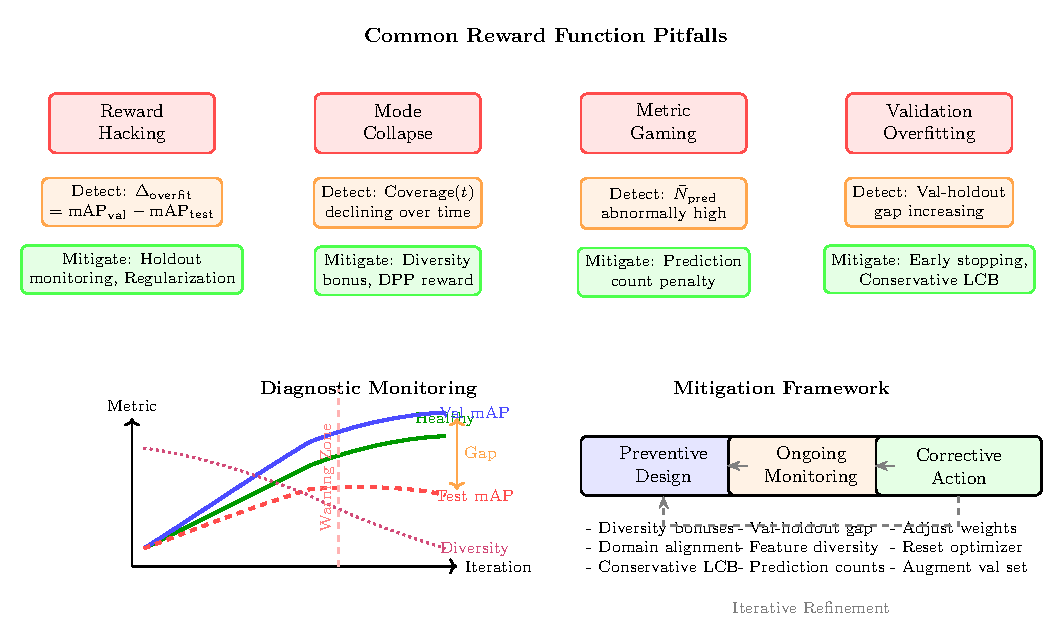
\includegraphics[width=\textwidth]{figures/ch07_fig4_pitfalls.pdf}
\caption{Common reward function pitfalls and mitigation strategies. Top: Four major pitfalls (reward hacking, mode collapse, metric gaming, and validation overfitting) with their detection metrics and mitigation approaches. Bottom left: Diagnostic monitoring showing the divergence between validation mAP (potentially overfitting) and test mAP, along with declining diversity indicating mode collapse. Bottom right: Three-phase mitigation framework combining preventive design, ongoing monitoring, and corrective action in an iterative refinement loop.}
\label{fig:pitfalls}
\end{figure}

\subsection{Overfitting to Validation Set}

The small validation sets typical of synthetic data optimization scenarios create severe overfitting risk. Configurations that achieve high validation reward may exploit idiosyncrasies of the specific validation images rather than learning generally transferable generation strategies.

Holdout monitoring reserves a portion of available real images as a test set never used for reward computation:
\begin{equation}
\text{mAP}_{\text{holdout}}(\theta) = \text{mAP}(\mathcal{D}_{\text{holdout}}, f_{\phi(\theta)})
\label{eq:holdout_map}
\end{equation}

Periodic evaluation on the holdout set (without using results for optimization) enables detection of validation overfitting.

Regularization through reward penalty terms discourages configurations that deviate excessively from prior knowledge:
\begin{equation}
r_{\text{regularized}} = r_{\text{mAP}} - \lambda_{\text{reg}} \|\theta - \theta_0\|^2
\label{eq:regularization}
\end{equation}
where $\theta_0$ represents a default or previously successful configuration.

Early stopping terminates optimization when validation performance plateaus while auxiliary metrics suggest declining quality:
\begin{equation}
\text{Stop if } \frac{d\text{mAP}_{\text{val}}}{dt} < \epsilon_{\text{stop}} \text{ and } \frac{d\text{Diversity}}{dt} < 0
\label{eq:early_stopping}
\end{equation}

\subsection{Shortcut Learning}

Shortcut learning occurs when detectors trained on synthetic data learn to exploit superficial correlations rather than semantically meaningful features. Common shortcuts include background texture correlations, object-background co-occurrence patterns, and rendering artifacts that distinguish synthetic from real images.

Diagnostic evaluation requires probing detector behavior under controlled perturbations. Background randomization tests whether the detector relies on background features:
\begin{equation}
\Delta_{\text{bg}} = \text{mAP}(\mathcal{D}_{\text{original}}) - \text{mAP}(\mathcal{D}_{\text{bg-random}})
\label{eq:background_sensitivity}
\end{equation}

Large $\Delta_{\text{bg}}$ indicates problematic background dependence.

Object-only evaluation tests detector performance on images with objects isolated from their original backgrounds, revealing whether the detector has learned object-intrinsic features or relies on contextual cues.

Mitigation strategies include aggressive background domain randomization in the synthetic data generator, explicit penalties for background sensitivity in the reward function, and multi-environment training that exposes detectors to varied contexts for the same objects.

\subsection{Mitigation Strategy Summary}

Effective mitigation of reward function pitfalls requires a multi-pronged approach combining preventive design, ongoing monitoring, and corrective interventions.

Preventive design incorporates diversity bonuses, domain alignment rewards, and conservative reward estimation from the outset, reducing the optimizer's ability to exploit reward function weaknesses.

Ongoing monitoring tracks diagnostic metrics including the validation-holdout gap, prediction count statistics, feature diversity, and parameter space variance. Automated alerts trigger when metrics exceed thresholds indicative of pathological behavior.

Corrective interventions include reward function adjustment (increasing diversity or exploration weights), optimizer reset to diverse initial conditions, and augmentation of the validation set when possible.

\section{Implementation Considerations}
\label{sec:implementation}

The translation of mathematical reward formulations into practical implementations requires attention to numerical stability, computational efficiency, and integration with existing machine learning infrastructure. This section addresses key implementation considerations that ensure reliable reward computation in production systems.

\subsection{Reward Normalization}

Effective reward normalization requires careful initialization and adaptation strategies to handle the non-stationary reward distributions encountered during optimization.

Burn-in initialization collects reward statistics during an initial exploration phase before applying normalization:
\begin{equation}
\mu_i^{(0)} = \frac{1}{T_{\text{burn}}} \sum_{t=1}^{T_{\text{burn}}} r_i(t), \quad \sigma_i^{(0)} = \sqrt{\frac{1}{T_{\text{burn}}-1} \sum_{t=1}^{T_{\text{burn}}} (r_i(t) - \mu_i^{(0)})^2}
\label{eq:burnin_initialization}
\end{equation}

During the burn-in period, unnormalized rewards are used, accepting higher variance in exchange for accurate initialization.

Adaptation rate scheduling adjusts the EMA parameter $\beta$ over time, using faster adaptation early (lower $\beta$) and slower adaptation later (higher $\beta$):
\begin{equation}
\beta(t) = \beta_{\text{final}} - (\beta_{\text{final}} - \beta_{\text{init}}) \exp(-t / \tau_\beta)
\label{eq:beta_schedule}
\end{equation}

Per-component normalization applies different strategies to different reward components based on their distributional characteristics. Bounded components (e.g., mAP $\in [0,1]$) may use min-max normalization, while unbounded components (e.g., MMD distances) require z-score normalization.

\subsection{Value Baseline for Variance Reduction}

When using policy gradient methods for optimization, a learned value baseline reduces gradient variance while maintaining unbiased gradient estimates. The baseline $V(s)$ estimates expected future reward from state $s$.

The advantage function quantifies how much better an action is relative to the baseline expectation:
\begin{equation}
A(s, a) = R(s, a) - V(s)
\label{eq:advantage}
\end{equation}

Using advantages rather than raw rewards in policy gradient updates substantially reduces variance:
\begin{equation}
\nabla_\theta J(\theta) = \mathbb{E}\left[ A(s, a) \nabla_\theta \log \pi_\theta(a|s) \right]
\label{eq:advantage_gradient}
\end{equation}

The value function can be parameterized as a neural network $V_\psi(s)$ trained to minimize temporal difference error:
\begin{equation}
\mathcal{L}_V(\psi) = \mathbb{E}\left[ (R(s, a) + \gamma V_\psi(s') - V_\psi(s))^2 \right]
\label{eq:value_loss}
\end{equation}

In synthetic data optimization, the state representation may include summary statistics of recent configurations, historical performance metrics, and remaining budget information.

\subsection{Clipping and Scaling}

Reward clipping prevents extreme values from destabilizing learning, while scaling ensures appropriate gradient magnitudes.

Hard clipping bounds rewards to a fixed interval:
\begin{equation}
R_{\text{clipped}} = \max(\min(R, R_{\text{max}}), R_{\text{min}})
\label{eq:hard_clipping}
\end{equation}

Typical bounds are $R_{\text{min}} = -10$ and $R_{\text{max}} = 10$ after normalization.

Soft clipping using tanh provides smoother gradients near boundaries:
\begin{equation}
R_{\text{soft}} = R_{\text{max}} \cdot \tanh(R / R_{\text{max}})
\label{eq:soft_clipping}
\end{equation}

Huber-style clipping combines linear behavior near zero with bounded growth at extremes:
\begin{equation}
R_{\text{Huber}} = \begin{cases}
R & \text{if } |R| \leq \delta \\
\delta \cdot \text{sign}(R) \cdot (1 + \log(|R|/\delta)) & \text{otherwise}
\end{cases}
\label{eq:huber_clipping}
\end{equation}

Scale adjustment ensures that the effective learning rate remains appropriate as reward statistics evolve:
\begin{equation}
R_{\text{scaled}} = R / \max(\sigma_R, \sigma_{\text{min}})
\label{eq:scale_adjustment}
\end{equation}
where $\sigma_{\text{min}}$ prevents division by near-zero values.

\subsection{Numerical Stability}

Numerical stability requires careful handling of edge cases, appropriate precision, and defensive programming practices.

Division safety prevents division by zero or near-zero values:
\begin{equation}
\frac{a}{b} \to \frac{a}{b + \epsilon \cdot \text{sign}(b)}
\label{eq:safe_division}
\end{equation}
where $\epsilon = 10^{-8}$ is typical for float32 precision.

Logarithm safety handles arguments near zero:
\begin{equation}
\log(x) \to \log(\max(x, \epsilon))
\label{eq:safe_log}
\end{equation}

Exponential overflow prevention clips arguments before exponentiation:
\begin{equation}
\exp(x) \to \exp(\min(x, 80))
\label{eq:safe_exp}
\end{equation}

For softmax operations, the log-sum-exp trick maintains precision:
\begin{equation}
\log \sum_i \exp(x_i) = x_{\max} + \log \sum_i \exp(x_i - x_{\max})
\label{eq:logsumexp}
\end{equation}

Mixed precision considerations arise when using float16 for efficiency. Reward computations should generally use float32 to maintain precision, with conversion only for final storage or communication.

Gradient checkpointing for long-horizon reward computation trades memory for computation, recomputing intermediate values during backpropagation rather than storing them. This is particularly relevant when reward computation involves backpropagation through the detector training process.

\section{Chapter Summary}

This chapter has developed a comprehensive framework for reward function engineering in the context of synthetic data optimization for object detection. The presentation began with the mathematical formulation of mean Average Precision and its component metrics, establishing the primary reward signal that guides optimization toward improved detector performance. The treatment of small validation sets introduced bootstrap confidence estimation and cross-validation strategies that address the statistical challenges inherent in scenarios with limited real-world imagery, providing principled approaches to variance reduction and conservative reward estimation.

The discussion of reward shaping strategies developed intermediate reward signals based on training dynamics, curriculum-based schedules that progressively increase evaluation stringency, and multi-objective balancing techniques that integrate competing objectives. The theoretical foundation of potential-based reward shaping ensures that shaped rewards preserve optimal policies while accelerating learning.

Auxiliary reward components address failure modes not captured by detection metrics alone, including diversity bonuses that prevent mode collapse, domain alignment rewards based on Maximum Mean Discrepancy that encourage distributional similarity to real data, and intrinsic motivation signals that promote systematic exploration of the parameter space. Efficiency rewards manage computational budgets while maintaining focus on detection quality.

The complete composite reward formulation integrates all components with appropriate normalization and temporal smoothing, providing stable learning signals throughout optimization. The analysis of reward function pitfalls cataloged common failure modes including reward hacking, mode collapse, and validation set overfitting, along with detection techniques and mitigation strategies.

Implementation considerations addressed the practical challenges of reward normalization, value baseline construction for variance reduction, clipping and scaling strategies, and numerical stability requirements. The algorithms and mathematical formulations presented provide a complete specification for implementing robust reward computation in production synthetic data optimization systems.

The reward function engineering principles developed in this chapter provide the foundation for effective reinforcement learning optimization of synthetic data generation parameters. When properly implemented, the composite reward function enables discovery of generator configurations that yield detectors achieving superior real-world performance while maintaining robustness against the pathological behaviors that can arise when optimizing complex, high-dimensional systems under limited supervision.


% Chapter 8: Sample Efficiency and Optimization
\chapter{Sample Efficiency and Multi-Fidelity Optimization}
\label{ch:sample_efficiency}
% Chapter 8: Sample Efficiency and Multi-Fidelity Optimization
% IEEE-Style Academic Textbook Chapter


\begin{abstract}
The optimization of synthetic data generation parameters for object detection models presents a fundamentally challenging sample efficiency problem. Each evaluation of a candidate parameter configuration requires generating synthetic images, training a deep neural network such as YOLO, and evaluating performance on real-world validation data. This computational pipeline renders traditional reinforcement learning approaches, which typically require millions of environment interactions, entirely impractical. This chapter develops a comprehensive framework for sample-efficient optimization in this expensive black-box setting, introducing multi-fidelity techniques, adaptive budget allocation strategies, and principled convergence detection methods that collectively enable effective optimization within strict computational constraints.
\end{abstract}

\section{The Sample Efficiency Challenge}
\label{sec:sample_efficiency_challenge}

The synthesis of training data for deep learning models through parametric generators introduces an optimization problem of considerable computational complexity. Unlike conventional hyperparameter tuning where model training represents the primary computational burden, synthetic data optimization compounds this cost with additional data generation overhead and the fundamental challenge of evaluating transfer performance from synthetic to real domains. Understanding the precise cost structure of this optimization problem is essential for designing algorithms that can achieve meaningful results within practical resource constraints.

\subsection{Cost Model for Synthetic Data Optimization}
\label{subsec:cost_model}

The total computational cost of evaluating a single configuration $\theta$ in the synthetic data optimization pipeline can be decomposed into three primary components. Let $C_{\text{gen}}(\theta, n)$ denote the cost of generating $n$ synthetic images with parameters $\theta$, $C_{\text{train}}(n, e)$ the cost of training the object detection model on $n$ images for $e$ epochs, and $C_{\text{eval}}$ the cost of evaluating the trained model on the real-world validation set. The total evaluation cost becomes:

\begin{equation}
C_{\text{total}}(\theta) = C_{\text{gen}}(\theta, n) + C_{\text{train}}(n, e) + C_{\text{eval}}
\label{eq:total_cost}
\end{equation}

For modern object detection architectures such as YOLOv8, training on a dataset of 5,000 synthetic images for 100 epochs on a contemporary GPU requires approximately 2-4 hours of wall-clock time. When multiplied across the hundreds of evaluations typically required for black-box optimization, the total computational budget can easily exceed thousands of GPU-hours. This cost structure fundamentally differentiates synthetic data optimization from conventional machine learning hyperparameter tuning, where individual evaluations may complete in minutes rather than hours.

The generation cost $C_{\text{gen}}(\theta, n)$ depends critically on the complexity of the synthetic data pipeline. Procedural generation systems based on domain randomization typically exhibit linear scaling with dataset size, while physics-based rendering engines may introduce substantial per-image overhead. For rendering engines such as BlenderProc or NVIDIA Isaac Sim, generating photorealistic synthetic images can require 1-10 seconds per image depending on scene complexity, material properties, and lighting configurations. A dataset of 5,000 images thus requires 1.5-14 hours of generation time, representing a non-negligible fraction of the total evaluation cost.

\subsection{Comparison with Traditional Reinforcement Learning}

Traditional deep reinforcement learning algorithms exhibit sample complexities that are fundamentally incompatible with the synthetic data optimization setting. Proximal Policy Optimization and similar policy gradient methods typically require $10^6$ to $10^9$ environment interactions to learn effective policies in continuous control tasks. Model-free approaches such as Deep Q-Networks demonstrate comparable sample requirements, with successful Atari game playing requiring approximately $10^8$ frames of experience.

The synthetic data optimization problem admits at most $10^2$ to $10^3$ evaluations within reasonable computational budgets, representing a gap of four to seven orders of magnitude relative to conventional reinforcement learning requirements. This disparity motivates the adoption of fundamentally different algorithmic approaches designed specifically for expensive black-box optimization. Bayesian optimization and its multi-fidelity extensions provide the theoretical foundation for achieving meaningful optimization progress within such severely constrained evaluation budgets.

Model-based reinforcement learning offers potential improvements in sample efficiency through the construction of learned dynamics models that enable policy optimization through simulated rollouts. World model approaches such as DreamerV3 have demonstrated the ability to learn complex behaviors with substantially reduced environment interactions, achieving near-optimal performance in some domains with as few as $5 \times 10^4$ interactions. However, even these improved sample complexities remain orders of magnitude beyond what the synthetic data optimization setting permits, necessitating further algorithmic innovations.

Figure~\ref{fig:sample_efficiency_comparison} illustrates the stark difference in sample requirements between traditional reinforcement learning approaches and the multi-fidelity methods developed in this chapter.

\begin{figure}[htbp]
\centering
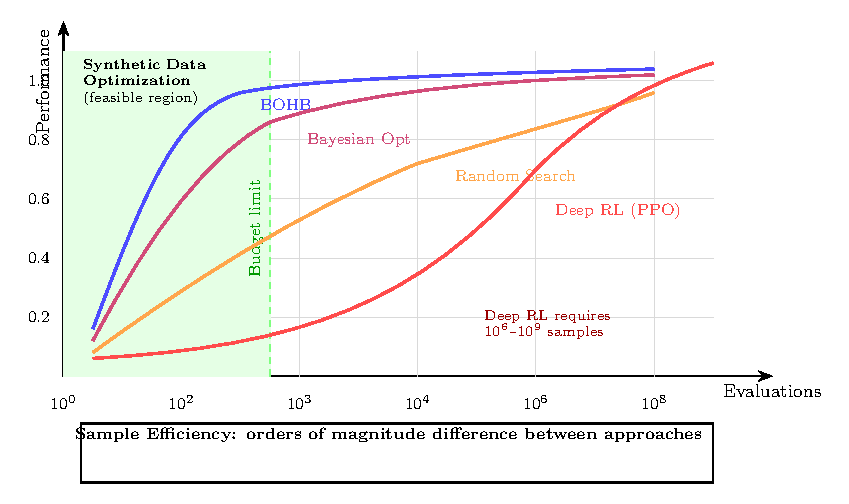
\includegraphics[width=0.85\textwidth]{figures/ch08_fig3_sample_efficiency.pdf}
\caption{Sample efficiency comparison across optimization approaches. Traditional deep reinforcement learning methods (e.g., PPO) require $10^6$--$10^9$ evaluations, far exceeding the feasible budget for synthetic data optimization. Multi-fidelity methods like BOHB achieve competitive performance within the practical budget limit of $10^2$--$10^3$ evaluations, representing a four to seven order-of-magnitude improvement in sample efficiency.}
\label{fig:sample_efficiency_comparison}
\end{figure}

\subsection{Budget Constraints in Practice}

Practical synthetic data optimization projects operate under multiple interacting constraints that collectively define the feasible optimization budget. Hardware availability determines the maximum parallelism achievable during evaluation, with typical academic and industrial settings providing access to 1-8 GPUs for sustained optimization campaigns. Project timelines impose wall-clock time limits that, combined with per-evaluation durations, bound the total number of sequential evaluations. Financial considerations in cloud computing environments translate directly to evaluation count limits through hourly GPU rental costs.

A representative budget for a synthetic data optimization project targeting industrial deployment might allocate 100-200 GPU-hours to the optimization process. With per-evaluation costs of 2-4 GPU-hours for full-fidelity training, this budget permits only 25-100 complete evaluations. The multi-fidelity techniques developed in subsequent sections enable more effective utilization of this limited budget by strategically allocating resources across evaluations of varying computational cost.

\section{Multi-Fidelity Optimization Framework}
\label{sec:multi_fidelity_framework}

Multi-fidelity optimization exploits the observation that expensive objective functions often admit cheaper approximations that correlate with the true objective. In the synthetic data optimization context, these approximations arise naturally through reduced training duration and smaller dataset sizes, both of which decrease computational cost while providing informative signals about configuration quality.

\subsection{Fidelity Dimensions}

The synthetic data optimization pipeline admits multiple independent dimensions along which fidelity can be varied. The training epoch dimension controls the number of complete passes through the training dataset, with early-epoch performance providing a noisy but correlated estimate of final performance. The dataset size dimension controls the number of synthetic images generated and used for training, with smaller datasets enabling faster generation and training at the cost of increased variance in the resulting model quality.

Formally, we extend the objective function to incorporate fidelity parameters:

\begin{equation}
f(\theta, r) : \Theta \times \mathcal{R} \rightarrow \mathbb{R}
\label{eq:multi_fidelity_objective}
\end{equation}

where $r = (r_{\text{epochs}}, r_{\text{data}}) \in \mathcal{R}$ represents the fidelity configuration and $\mathcal{R} = [r_{\min}^{\text{epochs}}, r_{\max}^{\text{epochs}}] \times [r_{\min}^{\text{data}}, r_{\max}^{\text{data}}]$ defines the fidelity space. The cost function $c(\theta, r)$ increases monotonically with both fidelity dimensions, while the correlation between $f(\theta, r)$ and the true objective $f(\theta, r_{\max})$ generally increases with fidelity.

\subsection{Fidelity Level Definitions}

Effective multi-fidelity optimization requires careful definition of discrete fidelity levels that balance computational cost against information quality. Table~\ref{tab:fidelity_levels} presents recommended fidelity configurations for synthetic data optimization with YOLO-family architectures, based on empirical observations of the cost-correlation tradeoff.

\begin{table}[htbp]
\centering
\caption{Multi-Fidelity Level Definitions for Synthetic Data Optimization}
\label{tab:fidelity_levels}
\begin{tabular}{lcccc}
\hline
\textbf{Fidelity Level} & \textbf{Epochs} & \textbf{Dataset Size} & \textbf{Relative Cost} & \textbf{Correlation} \\
\hline
Ultra-Low & 10 & 500 & 0.02 & 0.55--0.65 \\
Low & 25 & 1,000 & 0.08 & 0.70--0.80 \\
Medium & 50 & 2,500 & 0.25 & 0.85--0.90 \\
High & 100 & 5,000 & 1.00 & 1.00 \\
\hline
\end{tabular}
\end{table}

The correlation values in Table~\ref{tab:fidelity_levels} represent empirically observed rank correlations between configuration performance at each fidelity level and full-fidelity performance. These correlations exhibit substantial task dependence, with simpler detection problems showing higher correlations at lower fidelities while complex multi-class detection scenarios may require higher minimum fidelities for reliable configuration comparison.

Figure~\ref{fig:fidelity_pyramid} provides a visual representation of the multi-fidelity hierarchy, illustrating the tradeoff between computational cost and correlation with full-fidelity performance.

\begin{figure}[htbp]
\centering
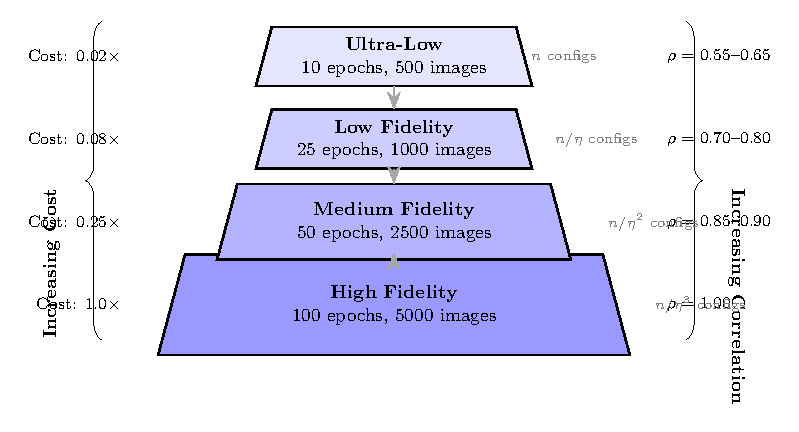
\includegraphics[width=0.85\textwidth]{figures/ch08_fig1_fidelity_pyramid.pdf}
\caption{Multi-fidelity evaluation pyramid showing the cost-correlation tradeoff across fidelity levels. Lower fidelity levels (top) evaluate many configurations at low cost but with reduced correlation to full-fidelity performance. Higher fidelity levels (bottom) provide accurate performance estimates but at substantially greater computational expense. The progressive filtering strategy evaluates $n$ configurations at ultra-low fidelity, promoting only the top $1/\eta$ fraction to each subsequent level.}
\label{fig:fidelity_pyramid}
\end{figure}

\subsection{Correlation Between Fidelity Levels}

The effectiveness of multi-fidelity optimization depends critically on the correlation structure between low-fidelity and high-fidelity evaluations. Let $\rho(r_1, r_2)$ denote the Spearman rank correlation between configuration rankings at fidelity levels $r_1$ and $r_2$. Effective multi-fidelity optimization requires $\rho(r_{\text{low}}, r_{\text{high}}) > 0.5$ to ensure that low-fidelity evaluations provide meaningful guidance for configuration selection.

Empirical studies of neural network hyperparameter optimization have demonstrated that early-epoch performance correlates strongly with final performance for many architecture and optimization configurations. This correlation arises from the learning dynamics of stochastic gradient descent, where configurations that learn rapidly in early epochs tend to maintain their relative advantage through continued training. However, pathological cases exist where early performance inversely correlates with final performance, particularly for configurations with aggressive learning rates that achieve rapid initial progress but subsequently diverge.

The dataset size dimension exhibits more complex correlation behavior. Reducing dataset size increases the variance of learned models due to reduced coverage of the underlying data distribution, potentially causing rank reversals between configurations. The impact is particularly pronounced for synthetic data optimization, where dataset diversity directly influences the model's ability to generalize to real-world data. Configurations that perform well on small synthetic datasets may fail to transfer effectively when scaled to larger training sets if they exploit spurious correlations in the limited data.

\subsection{Optimal Fidelity Scheduling}

The allocation of computational budget across fidelity levels represents a critical design decision in multi-fidelity optimization. Aggressive use of low-fidelity evaluations maximizes the number of configurations explored but risks discarding promising configurations due to noisy low-fidelity estimates. Conservative strategies that emphasize high-fidelity evaluations provide more reliable performance estimates but explore fewer configurations within a fixed budget.

Theoretical analysis of multi-fidelity Bayesian optimization suggests that optimal budget allocation depends on the cost ratio between fidelity levels and the correlation structure of the objective function. When low-fidelity evaluations are substantially cheaper than high-fidelity evaluations and exhibit strong correlation, aggressive allocation to low-fidelity exploration followed by selective high-fidelity validation maximizes expected optimization performance. The successive halving and Hyperband algorithms, developed in subsequent sections, provide principled approaches to this allocation problem.

% TikZ diagram for multi-fidelity evaluation flow
\begin{figure}[htbp]
\centering
\begin{tikzpicture}[
    node distance=1.5cm,
    box/.style={rectangle, draw, rounded corners, minimum width=2.5cm, minimum height=0.8cm, align=center, fill=blue!10},
    decision/.style={diamond, draw, aspect=2, minimum width=2cm, fill=yellow!20},
    arrow/.style={->, >=stealth, thick}
]
    % Nodes
    \node[box] (sample) {Sample\\Configuration $\theta$};
    \node[box, below=of sample] (lowfid) {Low-Fidelity\\Evaluation};
    \node[decision, below=of lowfid] (promote1) {Top\\$1/\eta$?};
    \node[box, below=of promote1] (medfid) {Medium-Fidelity\\Evaluation};
    \node[decision, below=of medfid] (promote2) {Top\\$1/\eta$?};
    \node[box, below=of promote2] (highfid) {High-Fidelity\\Evaluation};
    \node[box, right=3cm of promote1] (discard1) {Discard\\Configuration};
    \node[box, right=3cm of promote2] (discard2) {Discard\\Configuration};

    % Arrows
    \draw[arrow] (sample) -- (lowfid);
    \draw[arrow] (lowfid) -- (promote1);
    \draw[arrow] (promote1) -- node[left] {Yes} (medfid);
    \draw[arrow] (promote1) -- node[above] {No} (discard1);
    \draw[arrow] (medfid) -- (promote2);
    \draw[arrow] (promote2) -- node[left] {Yes} (highfid);
    \draw[arrow] (promote2) -- node[above] {No} (discard2);

    % Labels
    \node[left=0.5cm of lowfid, align=right] {Cost: $c_{\min}$\\Configs: $n$};
    \node[left=0.5cm of medfid, align=right] {Cost: $\eta \cdot c_{\min}$\\Configs: $n/\eta$};
    \node[left=0.5cm of highfid, align=right] {Cost: $\eta^2 \cdot c_{\min}$\\Configs: $n/\eta^2$};
\end{tikzpicture}
\caption{Multi-fidelity evaluation flow with progressive resource allocation. Configurations are evaluated at increasing fidelity levels, with only the top $1/\eta$ fraction promoted at each stage. This structure enables exploration of many configurations while concentrating computational resources on the most promising candidates.}
\label{fig:multi_fidelity_flow}
\end{figure}

\section{Successive Halving Algorithm}
\label{sec:successive_halving}

Successive halving provides a principled approach to multi-fidelity hyperparameter optimization by iteratively eliminating the worst-performing configurations while increasing the resource allocation to survivors. The algorithm achieves provable efficiency gains over uniform allocation strategies when low-fidelity evaluations correlate with high-fidelity performance.

\subsection{Mathematical Foundation}

Consider the problem of identifying the best configuration from a set of $n$ candidates, where each configuration $\theta_i$ has unknown quality $f(\theta_i)$ that can only be observed through noisy evaluations at varying fidelity levels. The successive halving algorithm operates under a total budget constraint $B$ and seeks to maximize the probability of correctly identifying the best configuration.

Let $r_{\min}$ denote the minimum resource allocation per configuration and $r_{\max}$ the maximum allocation required for reliable evaluation. The algorithm proceeds in $K = \lfloor \log_\eta(r_{\max}/r_{\min}) \rfloor$ rounds, where $\eta > 1$ is the elimination rate. At each round $k$, the algorithm evaluates remaining configurations with resource allocation $r_k = r_{\min} \cdot \eta^k$ and eliminates the bottom $(1 - 1/\eta)$ fraction based on observed performance.

The total resource consumption of successive halving can be bounded as:

\begin{equation}
B_{\text{SH}} = \sum_{k=0}^{K} n_k \cdot r_k = \sum_{k=0}^{K} \frac{n}{\eta^k} \cdot r_{\min} \cdot \eta^k = (K+1) \cdot n \cdot r_{\min}
\label{eq:sh_budget}
\end{equation}

where $n_k = n/\eta^k$ denotes the number of configurations remaining at round $k$. This budget scales linearly with the initial number of configurations and logarithmically with the fidelity range $r_{\max}/r_{\min}$, enabling exploration of large configuration spaces within modest computational budgets.

\subsection{Algorithm Description}

The successive halving algorithm proceeds through a sequence of elimination rounds, progressively focusing computational resources on promising configurations while discarding those exhibiting poor early performance. Algorithm~\ref{alg:successive_halving} presents the complete procedure.

\begin{algorithm}[htbp]
\caption{Successive Halving for Multi-Fidelity Optimization}
\label{alg:successive_halving}
\begin{algorithmic}[1]
\Require Configuration space $\Theta$, number of configurations $n$, minimum resource $r_{\min}$, maximum resource $r_{\max}$, elimination rate $\eta$
\Ensure Best configuration $\theta^*$
\State $K \gets \lfloor \log_\eta(r_{\max}/r_{\min}) \rfloor$ \Comment{Number of rounds}
\State $S_0 \gets \text{SampleConfigurations}(\Theta, n)$ \Comment{Initial configuration set}
\For{$k = 0, 1, \ldots, K$}
    \State $r_k \gets r_{\min} \cdot \eta^k$ \Comment{Resource allocation for round $k$}
    \State $n_k \gets |S_k|$ \Comment{Number of surviving configurations}
    \For{each $\theta \in S_k$}
        \State $v_\theta \gets \text{Evaluate}(\theta, r_k)$ \Comment{Evaluate at current fidelity}
    \EndFor
    \State $S_{k+1} \gets \text{TopFraction}(S_k, 1/\eta, \{v_\theta\})$ \Comment{Keep top $1/\eta$ fraction}
\EndFor
\State $\theta^* \gets \arg\max_{\theta \in S_K} v_\theta$ \Comment{Return best configuration}
\State \Return $\theta^*$
\end{algorithmic}
\end{algorithm}

The \textsc{SampleConfigurations} procedure generates initial configurations through random sampling or quasi-random sequences such as Sobol or Halton. The \textsc{Evaluate} function executes the synthetic data optimization pipeline with the specified configuration and resource allocation, returning the observed performance metric. The \textsc{TopFraction} procedure sorts configurations by observed performance and retains only the top $1/\eta$ fraction for subsequent rounds.

\subsection{Bracket Configuration}

The successive halving algorithm requires specification of four primary hyperparameters that collectively determine its behavior. The initial configuration count $n$ controls the breadth of exploration, with larger values enabling evaluation of more diverse configurations at the cost of reduced per-configuration resources. The elimination rate $\eta$ determines the aggressiveness of pruning, with typical values ranging from 2 to 4. Smaller values of $\eta$ result in more gradual elimination but require additional rounds, while larger values enable faster convergence at the risk of prematurely discarding good configurations.

The minimum and maximum resource allocations $r_{\min}$ and $r_{\max}$ define the fidelity range over which the algorithm operates. The minimum allocation should be chosen to provide sufficient signal for meaningful configuration comparison while minimizing computational cost. For synthetic data optimization with YOLO, empirical evidence suggests $r_{\min}$ corresponding to 10-25 training epochs on 500-1,000 images provides adequate discrimination between configurations.

\subsection{Resource Allocation Analysis}

The resource allocation strategy of successive halving exhibits favorable theoretical properties when the objective function satisfies certain regularity conditions. Under the assumption that low-fidelity rankings correlate perfectly with high-fidelity rankings, successive halving identifies the optimal configuration with probability 1 while consuming resources logarithmic in the number of initial configurations.

More realistic analysis accounts for rank correlation degradation at low fidelities. Let $\epsilon$ denote the probability that a configuration's rank changes by more than $1/\eta$ fraction between adjacent fidelity levels. The success probability of successive halving degrades gracefully with $\epsilon$, maintaining high accuracy when $\epsilon < 1/\eta$. This analysis motivates the choice of conservative elimination rates in settings where low-fidelity correlation is uncertain.

% TikZ diagram for successive halving bracket structure
\begin{figure}[htbp]
\centering
\begin{tikzpicture}[
    scale=0.9,
    config/.style={circle, draw, minimum size=0.4cm, inner sep=0, fill=blue!30},
    eliminated/.style={circle, draw, minimum size=0.4cm, inner sep=0, fill=red!20, draw=red!50},
    rung/.style={thick}
]
    % Rung labels
    \node[anchor=east] at (-0.5, 0) {$r_0 = r_{\min}$};
    \node[anchor=east] at (-0.5, -2) {$r_1 = \eta \cdot r_{\min}$};
    \node[anchor=east] at (-0.5, -4) {$r_2 = \eta^2 \cdot r_{\min}$};
    \node[anchor=east] at (-0.5, -6) {$r_3 = r_{\max}$};

    % Rung lines
    \draw[rung] (0, 0) -- (13, 0);
    \draw[rung] (0, -2) -- (13, -2);
    \draw[rung] (0, -4) -- (13, -4);
    \draw[rung] (0, -6) -- (13, -6);

    % Round 0: 16 configurations
    \foreach \i in {1,...,16} {
        \pgfmathsetmacro{\x}{0.5 + (\i-1)*0.75}
        \node[config] (r0c\i) at (\x, 0) {};
    }

    % Round 1: 8 configurations (top half promoted)
    \foreach \i in {1,...,8} {
        \pgfmathsetmacro{\x}{1.5 + (\i-1)*1.25}
        \node[config] (r1c\i) at (\x, -2) {};
    }
    % Eliminated in round 0
    \foreach \i in {9,...,16} {
        \pgfmathsetmacro{\x}{0.5 + (\i-1)*0.75}
        \node[eliminated] at (\x, 0) {};
    }

    % Round 2: 4 configurations
    \foreach \i in {1,...,4} {
        \pgfmathsetmacro{\x}{3 + (\i-1)*2.5}
        \node[config] (r2c\i) at (\x, -4) {};
    }

    % Round 3: 2 configurations
    \foreach \i in {1,...,2} {
        \pgfmathsetmacro{\x}{5 + (\i-1)*4}
        \node[config] (r3c\i) at (\x, -6) {};
    }

    % Connection lines (sample)
    \draw[->, gray] (r0c1) -- (r1c1);
    \draw[->, gray] (r0c3) -- (r1c2);
    \draw[->, gray] (r0c5) -- (r1c3);
    \draw[->, gray] (r0c7) -- (r1c4);
    \draw[->, gray] (r1c1) -- (r2c1);
    \draw[->, gray] (r1c3) -- (r2c2);
    \draw[->, gray] (r2c1) -- (r3c1);
    \draw[->, gray] (r2c3) -- (r3c2);

    % Legend
    \node[config, label=right:Promoted] at (14, -1) {};
    \node[eliminated, label=right:Eliminated] at (14, -2) {};

    % Annotation
    \node[anchor=west, align=left] at (0, -7.5) {$\eta = 2$: Each round promotes top 50\% of configurations};
\end{tikzpicture}
\caption{Successive halving bracket structure with $n=16$ initial configurations and elimination rate $\eta=2$. Blue nodes represent configurations promoted to the next fidelity level, while red nodes indicate eliminated configurations. The algorithm requires $\log_\eta(n) = 4$ rounds to identify the final winner.}
\label{fig:sh_bracket}
\end{figure}

\section{Hyperband}
\label{sec:hyperband}

While successive halving provides an effective multi-fidelity optimization strategy, its performance depends critically on the choice of initial configuration count $n$. Choosing $n$ too small limits exploration of the configuration space, while choosing $n$ too large spreads resources thinly across initial low-fidelity evaluations. The Hyperband algorithm addresses this tradeoff by running multiple successive halving brackets with different initial configuration counts, automatically adapting to the unknown exploration-exploitation tradeoff.

\subsection{Extension of Successive Halving}

Hyperband operates by executing $s_{\max} + 1$ successive halving brackets in sequence, where each bracket $s \in \{0, 1, \ldots, s_{\max}\}$ uses a different initial configuration count and minimum resource allocation. The parameter $s_{\max} = \lfloor \log_\eta(r_{\max}/r_{\min}) \rfloor$ equals the maximum number of halving rounds possible within the fidelity range.

For bracket $s$, the algorithm initializes $n_s = \lceil (s_{\max}+1) \eta^s / (s+1) \rceil$ configurations with minimum resource allocation $r_s = r_{\max} \eta^{-s}$. This allocation scheme ensures that each bracket consumes approximately equal total resources while exploring different regions of the exploration-exploitation spectrum. Brackets with larger $s$ values explore more configurations at lower initial fidelities, while brackets with smaller $s$ values explore fewer configurations but provide each with higher initial resources.

\subsection{Multiple Bracket Strategy}

The multiple bracket strategy of Hyperband provides robustness to uncertainty about the optimal exploration-exploitation tradeoff. When low-fidelity evaluations strongly predict high-fidelity performance, brackets with large $s$ values (aggressive exploration) dominate performance by efficiently screening many configurations. When low-fidelity predictions are unreliable, brackets with small $s$ values (conservative exploration) succeed by providing configurations with sufficient resources for reliable evaluation.

The total resource consumption of a complete Hyperband iteration, executing all $s_{\max}+1$ brackets, can be bounded as:

\begin{equation}
B_{\text{HB}} \leq (s_{\max}+1)^2 \cdot r_{\max}
\label{eq:hb_budget}
\end{equation}

This resource consumption scales quadratically with the logarithm of the fidelity range, maintaining efficiency for large fidelity ranges while providing comprehensive coverage of the exploration-exploitation spectrum.

\subsection{Theoretical Guarantees}

Hyperband provides theoretical guarantees on optimization performance under mild regularity assumptions. Let $\nu$ denote the fraction of configurations with quality within $\epsilon$ of optimal. Under the assumption that low-fidelity rankings preserve the relative ordering of near-optimal configurations, Hyperband identifies an $\epsilon$-optimal configuration with high probability using resources:

\begin{equation}
B^* = O\left( \frac{r_{\max}}{\nu} \log\left(\frac{1}{\nu}\right) \log\left(\frac{r_{\max}}{r_{\min}}\right) \right)
\label{eq:hb_guarantee}
\end{equation}

This guarantee improves upon uniform random search, which requires $O(r_{\max}/\nu)$ resources, by a factor logarithmic in the fidelity range. The improvement becomes substantial when the fidelity range spans multiple orders of magnitude, as is typical in neural network training settings.

\subsection{Comparison with Pure Bayesian Optimization}

Pure Bayesian optimization constructs a probabilistic surrogate model of the objective function and uses this model to guide sequential configuration selection through an acquisition function. While Bayesian optimization achieves strong theoretical and empirical performance in low-dimensional continuous optimization, its advantages diminish in the multi-fidelity setting for several reasons.

First, Gaussian process surrogate models incur computational costs that scale cubically with the number of observations, limiting their applicability when hundreds or thousands of low-fidelity evaluations are collected. Second, extending Bayesian optimization to the multi-fidelity setting requires modeling the correlation structure between fidelity levels, introducing additional complexity and potential for model misspecification. Third, the sequential nature of Bayesian optimization limits parallelization opportunities, while successive halving and Hyperband naturally support parallel evaluation within each round.

Empirical comparisons across hyperparameter optimization benchmarks demonstrate that Hyperband matches or exceeds the performance of Gaussian process-based Bayesian optimization while providing substantially faster wall-clock convergence through parallelization. The BOHB algorithm, developed in the following section, combines the strengths of both approaches by using Bayesian optimization for configuration sampling within the Hyperband framework.

Figure~\ref{fig:hyperband_brackets} illustrates the complete bracket structure of Hyperband, showing how different brackets explore the configuration space with varying levels of aggressiveness.

\begin{figure}[htbp]
\centering
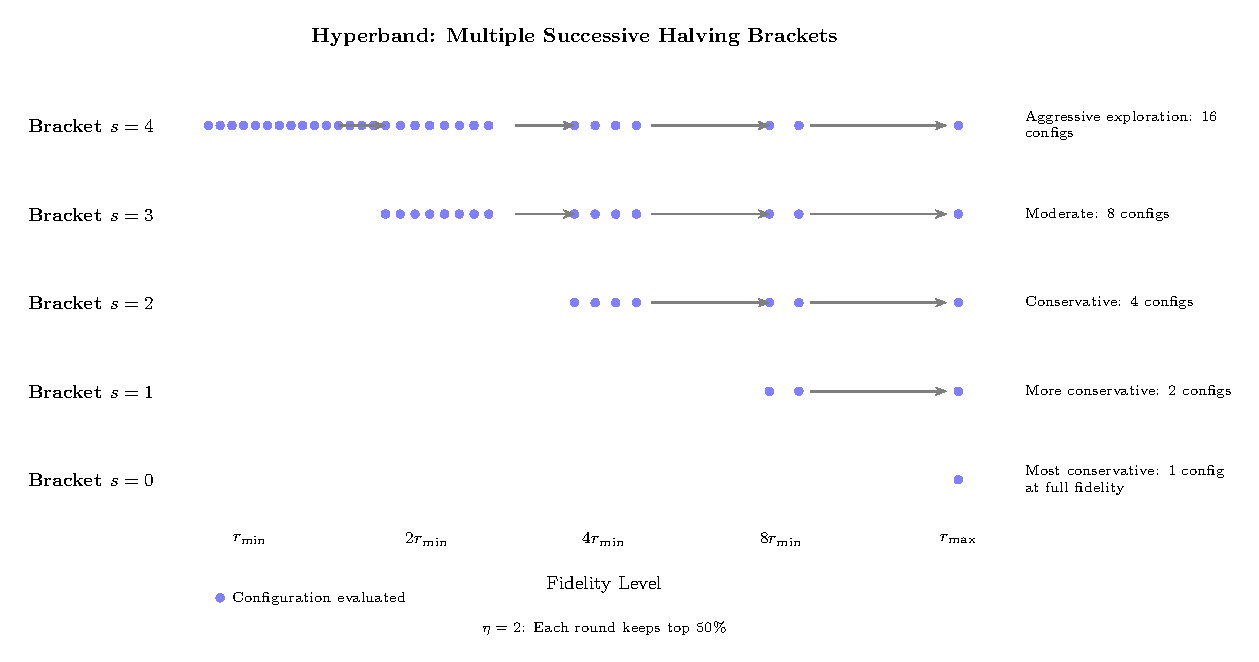
\includegraphics[width=0.95\textwidth]{figures/ch08_fig2_hyperband_brackets.pdf}
\caption{Hyperband bracket structure with $\eta = 2$ and $s_{\max} = 4$. Each row represents a different bracket with varying exploration-exploitation tradeoffs. Bracket $s=4$ (top) explores 16 configurations starting at minimum fidelity, aggressively filtering through successive halving. Bracket $s=0$ (bottom) evaluates a single configuration at maximum fidelity. The multiple bracket strategy provides robustness to uncertainty about optimal allocation between exploration and exploitation.}
\label{fig:hyperband_brackets}
\end{figure}

\begin{algorithm}[htbp]
\caption{Hyperband Algorithm}
\label{alg:hyperband}
\begin{algorithmic}[1]
\Require Configuration space $\Theta$, minimum resource $r_{\min}$, maximum resource $r_{\max}$, elimination rate $\eta$
\Ensure Best configuration $\theta^*$
\State $s_{\max} \gets \lfloor \log_\eta(r_{\max}/r_{\min}) \rfloor$
\State $B \gets (s_{\max} + 1) \cdot r_{\max}$ \Comment{Budget per Hyperband iteration}
\State $\theta^* \gets \text{null}$, $v^* \gets -\infty$
\For{$s = s_{\max}, s_{\max}-1, \ldots, 0$} \Comment{Outer loop over brackets}
    \State $n_s \gets \lceil \frac{B}{r_{\max}} \cdot \frac{\eta^s}{s+1} \rceil$ \Comment{Initial configurations for bracket $s$}
    \State $r_s \gets r_{\max} \cdot \eta^{-s}$ \Comment{Initial resource for bracket $s$}
    \State $S \gets \text{SampleConfigurations}(\Theta, n_s)$
    \For{$k = 0, 1, \ldots, s$} \Comment{Inner loop: successive halving}
        \State $n_k \gets \lfloor n_s \cdot \eta^{-k} \rfloor$
        \State $r_k \gets r_s \cdot \eta^k$
        \For{each $\theta \in S$}
            \State $v_\theta \gets \text{Evaluate}(\theta, r_k)$
            \If{$v_\theta > v^*$}
                \State $\theta^* \gets \theta$, $v^* \gets v_\theta$
            \EndIf
        \EndFor
        \State $S \gets \text{TopFraction}(S, 1/\eta, \{v_\theta\})$
    \EndFor
\EndFor
\State \Return $\theta^*$
\end{algorithmic}
\end{algorithm}

\section{BOHB: Combining Bayesian Optimization with Hyperband}
\label{sec:bohb}

The BOHB algorithm represents a sophisticated synthesis of Bayesian optimization and Hyperband that inherits the strengths of both approaches. By replacing the random configuration sampling of Hyperband with model-based sampling, BOHB achieves improved sample efficiency while maintaining the robustness and parallelization capabilities of the Hyperband framework.

\subsection{TPE Sampler Integration}

BOHB employs the Tree-structured Parzen Estimator as its surrogate model for configuration sampling. Unlike Gaussian process-based Bayesian optimization, which models the objective function directly, TPE models the conditional probability of configurations given their performance. Specifically, TPE maintains two density estimates: $\ell(\theta)$ modeling the density of configurations with performance above a threshold $\gamma$, and $g(\theta)$ modeling configurations below the threshold.

The acquisition function for TPE sampling takes the form:

\begin{equation}
\alpha(\theta) = \frac{\ell(\theta)}{g(\theta)}
\label{eq:tpe_acquisition}
\end{equation}

This ratio-based acquisition function naturally trades off exploration and exploitation by favoring configurations that are likely under the good-performance model $\ell(\theta)$ while unlikely under the poor-performance model $g(\theta)$. New configurations are sampled by drawing candidates from $\ell(\theta)$ and selecting those with highest acquisition values.

The computational efficiency of TPE derives from its kernel density estimation approach, which scales linearly with the number of observations rather than cubically as with Gaussian processes. This efficiency enables BOHB to effectively utilize the large number of low-fidelity observations generated by Hyperband's multiple brackets.

\subsection{Warm-Starting Strategies}

BOHB incorporates several warm-starting strategies to accelerate optimization by leveraging historical evaluation data. When optimizing a new synthetic data generation task, BOHB can initialize its TPE models using observations from related tasks, providing an informative prior that guides early exploration toward promising regions of the configuration space.

The multi-fidelity structure of BOHB enables sophisticated warm-starting through fidelity-conditional modeling. Observations from low-fidelity evaluations update the TPE models with appropriate weighting, providing dense coverage of the configuration space while allowing high-fidelity observations to dominate near-optimal configurations. This hierarchical modeling approach enables BOHB to efficiently allocate limited high-fidelity observations while maintaining comprehensive exploration through low-fidelity evaluations.

\subsection{Implementation with Optuna}

The Optuna hyperparameter optimization framework provides a production-ready implementation of BOHB that integrates seamlessly with Python-based machine learning workflows. Optuna's define-by-run API enables flexible specification of configuration spaces, including conditional parameters and hierarchical structures that frequently arise in synthetic data generation pipelines.

The following code fragment illustrates the integration of BOHB with Optuna for synthetic data optimization:

\begin{verbatim}
import optuna
from optuna.pruners import HyperbandPruner
from optuna.samplers import TPESampler

def objective(trial):
    # Define synthetic data parameters
    brightness_range = trial.suggest_float("brightness", 0.5, 1.5)
    contrast_range = trial.suggest_float("contrast", 0.5, 1.5)
    noise_level = trial.suggest_float("noise", 0.0, 0.1)

    # Multi-fidelity: report intermediate values
    for epoch in [10, 25, 50, 100]:
        mAP = train_and_evaluate(brightness_range, contrast_range,
                                  noise_level, epochs=epoch)
        trial.report(mAP, epoch)
        if trial.should_prune():
            raise optuna.TrialPruned()

    return mAP

study = optuna.create_study(
    direction="maximize",
    sampler=TPESampler(n_startup_trials=10),
    pruner=HyperbandPruner(min_resource=10, max_resource=100,
                           reduction_factor=3)
)
study.optimize(objective, n_trials=100)
\end{verbatim}

\subsection{Complete BOHB Algorithm}

Algorithm~\ref{alg:bohb} presents the complete BOHB procedure, integrating TPE-based configuration sampling with the Hyperband bracket structure.

\begin{algorithm}[htbp]
\caption{BOHB: Bayesian Optimization with Hyperband}
\label{alg:bohb}
\begin{algorithmic}[1]
\Require Configuration space $\Theta$, resource bounds $r_{\min}, r_{\max}$, elimination rate $\eta$, TPE quantile $\gamma$
\Ensure Best configuration $\theta^*$
\State $s_{\max} \gets \lfloor \log_\eta(r_{\max}/r_{\min}) \rfloor$
\State Initialize TPE models $\mathcal{M}_r$ for each fidelity level $r$
\State $\mathcal{D} \gets \emptyset$ \Comment{Observation history}
\State $\theta^* \gets \text{null}$, $v^* \gets -\infty$
\While{budget not exhausted}
    \For{$s = s_{\max}, s_{\max}-1, \ldots, 0$}
        \State $n_s \gets \lceil \frac{(s_{\max}+1) \eta^s}{s+1} \rceil$
        \State $r_s \gets r_{\max} \cdot \eta^{-s}$
        \State $S \gets \emptyset$
        \For{$i = 1, \ldots, n_s$}
            \If{$|\mathcal{D}| < n_{\text{startup}}$}
                \State $\theta \gets \text{RandomSample}(\Theta)$
            \Else
                \State $\theta \gets \text{TPESample}(\Theta, \mathcal{M}_{r_s}, \gamma)$
            \EndIf
            \State $S \gets S \cup \{\theta\}$
        \EndFor
        \For{$k = 0, 1, \ldots, s$}
            \State $r_k \gets r_s \cdot \eta^k$
            \For{each $\theta \in S$}
                \State $v_\theta \gets \text{Evaluate}(\theta, r_k)$
                \State $\mathcal{D} \gets \mathcal{D} \cup \{(\theta, r_k, v_\theta)\}$
                \State Update TPE model $\mathcal{M}_{r_k}$ with new observation
                \If{$r_k = r_{\max}$ and $v_\theta > v^*$}
                    \State $\theta^* \gets \theta$, $v^* \gets v_\theta$
                \EndIf
            \EndFor
            \State $S \gets \text{TopFraction}(S, 1/\eta, \{v_\theta\})$
        \EndFor
    \EndFor
\EndWhile
\State \Return $\theta^*$
\end{algorithmic}
\end{algorithm}

\section{Budget Allocation Strategy}
\label{sec:budget_allocation}

Effective utilization of limited computational resources requires careful planning of budget allocation across optimization phases. This section develops a comprehensive framework for budget planning in synthetic data optimization projects, providing concrete recommendations based on empirical observations and theoretical analysis.

\subsection{Recommended Phase Breakdown}

The optimization process naturally decomposes into three phases with distinct objectives and resource requirements. The exploration phase seeks to identify promising regions of the configuration space through broad, low-fidelity evaluation. The refinement phase narrows the search within identified promising regions using medium-fidelity evaluations. The validation phase provides high-confidence performance estimates for final configuration selection through full-fidelity evaluation.

Table~\ref{tab:phase_breakdown} presents recommended budget allocations for each phase under varying total budget constraints.

\begin{table}[htbp]
\centering
\caption{Recommended Budget Allocation by Optimization Phase}
\label{tab:phase_breakdown}
\begin{tabular}{lccc}
\hline
\textbf{Phase} & \textbf{Budget Share} & \textbf{Fidelity Level} & \textbf{Objective} \\
\hline
Exploration & 35--45\% & Low (10--25 epochs) & Identify promising regions \\
Refinement & 30--40\% & Medium (25--50 epochs) & Narrow candidate set \\
Validation & 20--30\% & High (100 epochs) & Final selection \\
\hline
\end{tabular}
\end{table}

The exploration phase consumes the largest budget fraction but at the lowest per-configuration cost, enabling evaluation of 50-200 diverse configurations. The refinement phase reduces the candidate set to 10-30 configurations while providing more reliable performance estimates. The validation phase concentrates resources on 5-15 finalist configurations to enable confident selection of the optimal configuration.

\subsection{Exploration vs. Validation Budget}

The allocation between exploration and validation phases represents a fundamental tradeoff in budget-constrained optimization. Allocating excessive budget to exploration maximizes configuration coverage but may fail to accurately rank top configurations due to limited high-fidelity evaluation. Conversely, allocating excessive budget to validation provides accurate rankings but only for a restricted set of configurations, risking exclusion of the global optimum.

Theoretical analysis suggests that optimal allocation depends on the shape of the configuration quality distribution. When good configurations are rare, exploration-heavy allocation increases the probability of encountering at least one good configuration. When good configurations are common, validation-heavy allocation maximizes the probability of correctly identifying the best among discovered configurations.

For synthetic data optimization, empirical evidence suggests that good configurations exist at moderate density in typical configuration spaces, supporting the balanced allocation in Table~\ref{tab:phase_breakdown}. Projects with highly constrained budgets should prioritize exploration to ensure sufficient configuration diversity, while projects with generous budgets can increase validation allocation to reduce selection uncertainty.

\subsection{Reserve Budget Considerations}

Practical optimization projects should maintain a reserve budget of 10-15\% of total resources to accommodate unexpected requirements. Common uses of reserve budget include extended evaluation of surprisingly good configurations discovered late in optimization, investigation of configuration sensitivity through replicated evaluations, and recovery from failed evaluations due to hardware or software issues.

The reserve budget also supports adaptive reallocation between phases based on intermediate results. If exploration reveals unexpectedly dense promising regions, reserve budget can fund additional refinement evaluations. Conversely, if promising configurations are sparse, reserve budget can extend the exploration phase.

\subsection{Total Resource Estimation Framework}

Table~\ref{tab:resource_estimation} provides a complete framework for estimating total resource requirements based on project parameters. The framework accounts for all cost components and provides confidence intervals reflecting uncertainty in individual evaluation costs.

\begin{table}[htbp]
\centering
\caption{Total Resource Estimation Framework for Synthetic Data Optimization}
\label{tab:resource_estimation}
\begin{tabular}{lccr}
\hline
\textbf{Phase} & \textbf{Configurations} & \textbf{Cost/Config (GPU-hr)} & \textbf{Phase Total} \\
\hline
Exploration (Low) & 100 & 0.3--0.5 & 30--50 GPU-hr \\
Refinement (Med) & 25 & 1.0--1.5 & 25--38 GPU-hr \\
Validation (High) & 10 & 3.0--4.0 & 30--40 GPU-hr \\
Reserve & -- & -- & 10--15 GPU-hr \\
\hline
\textbf{Total} & & & \textbf{95--143 GPU-hr} \\
\hline
\end{tabular}
\end{table}

This resource estimate assumes a dataset size of 5,000 images at full fidelity, 100 training epochs for high-fidelity evaluation, and a YOLO-medium architecture. Projects using larger datasets, longer training, or more complex architectures should scale estimates proportionally. Cloud computing costs at typical GPU rental rates of \$1-3 per GPU-hour translate this estimate to \$100-400 total project cost, demonstrating the economic feasibility of rigorous synthetic data optimization.

Figure~\ref{fig:budget_allocation} provides a visual summary of the three-phase budget allocation strategy and the configuration filtering funnel.

\begin{figure}[htbp]
\centering
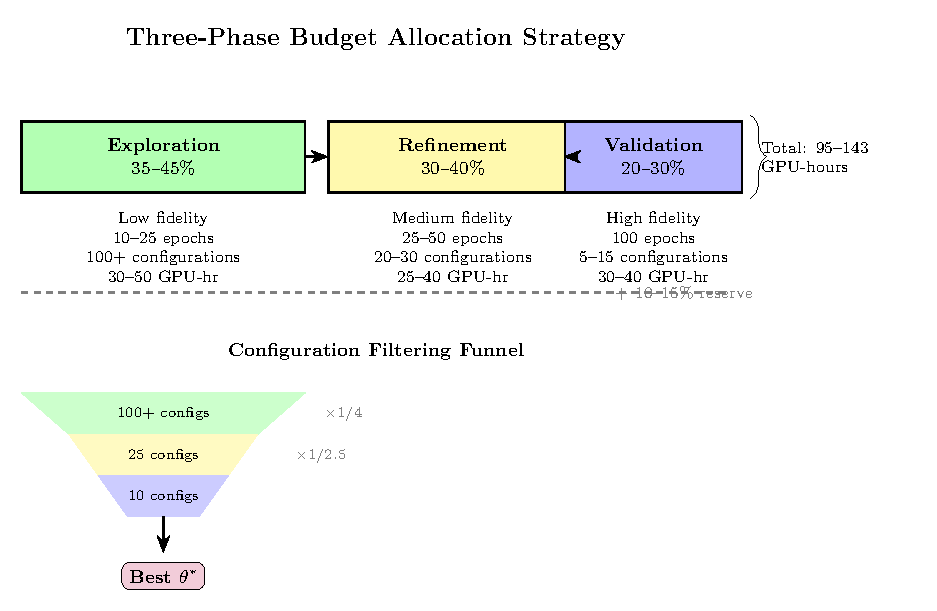
\includegraphics[width=0.9\textwidth]{figures/ch08_fig4_budget_allocation.pdf}
\caption{Three-phase budget allocation strategy for synthetic data optimization. The exploration phase (35--45\% of budget) evaluates 100+ configurations at low fidelity to identify promising regions. The refinement phase (30--40\%) narrows candidates to approximately 25 using medium-fidelity evaluation. The validation phase (20--30\%) provides high-confidence performance estimates for the 10 finalist configurations. A 10--15\% reserve accommodates unexpected requirements. The configuration filtering funnel (bottom) illustrates how progressive filtering concentrates resources on the most promising configurations.}
\label{fig:budget_allocation}
\end{figure}

\section{Convergence Detection}
\label{sec:convergence_detection}

Detecting convergence in black-box optimization is complicated by the inherent noise in objective function evaluations and the absence of gradient information. This section develops principled methods for convergence detection that enable early termination when further optimization is unlikely to yield meaningful improvement, conserving computational resources for subsequent experiments.

\subsection{Detecting Convergence in Noisy Settings}

The synthetic data optimization objective exhibits substantial evaluation noise arising from stochastic initialization, random sampling during training, and the inherent variability of performance metrics on finite validation sets. This noise complicates convergence detection by obscuring the underlying optimization trajectory.

Formal convergence in stochastic optimization is typically defined in terms of the distance to a stationary point of the expected objective. However, the black-box setting precludes computation of gradients or Hessians, necessitating convergence criteria based solely on observed objective values. A practical definition considers the optimization converged when the expected improvement from additional evaluations falls below a problem-specific threshold $\epsilon$.

Let $y_t^*$ denote the best observed objective value after $t$ evaluations. The optimization exhibits diminishing returns when:

\begin{equation}
\mathbb{E}[y_{t+\Delta}^* - y_t^* | \mathcal{D}_t] < \epsilon
\label{eq:convergence_criterion}
\end{equation}

where $\mathcal{D}_t$ represents the evaluation history and $\Delta$ denotes a lookahead horizon. Estimating this expectation requires modeling the objective function, which Bayesian optimization provides through its surrogate model.

\subsection{EMA-Based Stopping Criteria}

Exponential moving average filtering provides a robust approach to convergence detection that smooths noisy observations while maintaining sensitivity to recent improvements. Define the EMA of best observed values as:

\begin{equation}
\bar{y}_t = \alpha y_t^* + (1-\alpha) \bar{y}_{t-1}
\label{eq:ema_definition}
\end{equation}

where $\alpha \in (0, 1)$ controls the smoothing strength. The convergence criterion based on EMA improvement compares the current EMA to a lagged value:

\begin{equation}
\bar{y}_t - \bar{y}_{t-w} < \epsilon
\label{eq:ema_convergence}
\end{equation}

where $w$ is the lookback window size. This criterion triggers when the smoothed objective shows insufficient improvement over the lookback period.

The choice of smoothing parameter $\alpha$ and lookback window $w$ involves a tradeoff between responsiveness and robustness. Smaller $\alpha$ values (stronger smoothing) reduce false convergence detection due to noise but delay detection of true convergence. Typical values of $\alpha = 0.1$ to $0.3$ and $w = 10$ to $20$ evaluations provide good performance across optimization problems.

Figure~\ref{fig:convergence_detection} illustrates the convergence detection process, showing the relationship between raw observations, EMA smoothing, and convergence criteria.

\begin{figure}[htbp]
\centering
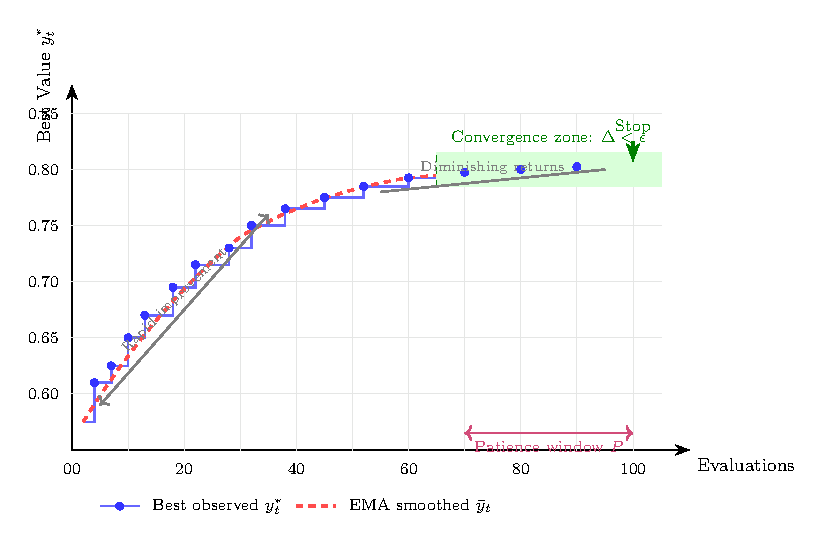
\includegraphics[width=0.85\textwidth]{figures/ch08_fig5_convergence_detection.pdf}
\caption{Convergence detection in sample-efficient optimization. The step function (solid blue) shows the best observed value $y_t^*$ over successive evaluations, with rapid improvement in early iterations followed by diminishing returns. The EMA-smoothed curve (dashed red) provides a noise-robust trajectory estimate. The convergence zone (green shaded region) indicates where improvement falls below threshold $\epsilon$. The patience window $P$ tracks evaluations without improvement, triggering termination when optimization has stagnated.}
\label{fig:convergence_detection}
\end{figure}

\subsection{Statistical Tests for Improvement}

Formal statistical testing provides rigorous convergence criteria with controlled false positive rates. The Mann-Whitney U test offers a nonparametric comparison between recent evaluations and historical evaluations, detecting whether recent observations come from a distribution with higher median.

Partition the evaluation history into recent observations $\{y_{t-w+1}, \ldots, y_t\}$ and historical observations $\{y_1, \ldots, y_{t-w}\}$. The null hypothesis $H_0$ asserts that recent observations are not stochastically greater than historical observations. Rejecting $H_0$ indicates continued improvement, while failing to reject suggests convergence.

The significance level $\alpha_{\text{test}}$ controls the false convergence rate, with typical values of 0.05 to 0.10 providing adequate sensitivity. When multiple statistical tests are performed across the optimization trajectory, appropriate corrections for multiple comparisons maintain the family-wise error rate.

\subsection{Patience-Based Early Stopping}

Patience-based stopping provides a simple yet effective convergence criterion that terminates optimization after a specified number of evaluations without improvement. Define the patience counter $p_t$ as:

\begin{equation}
p_t = \begin{cases}
0 & \text{if } y_t > y_{t-1}^* \\
p_{t-1} + 1 & \text{otherwise}
\end{cases}
\label{eq:patience_counter}
\end{equation}

The optimization terminates when $p_t$ exceeds the patience threshold $P$. This simple rule provides intuitive behavior while avoiding overfitting to noise when $P$ is chosen appropriately.

Algorithm~\ref{alg:convergence} presents a comprehensive convergence detection procedure that combines EMA-based, statistical, and patience-based criteria.

\begin{algorithm}[htbp]
\caption{Convergence Detection for Sample-Efficient Optimization}
\label{alg:convergence}
\begin{algorithmic}[1]
\Require Evaluation history $\mathcal{D} = \{(\theta_i, y_i)\}_{i=1}^t$, EMA parameter $\alpha$, lookback window $w$, improvement threshold $\epsilon$, patience $P$, significance level $\alpha_{\text{test}}$
\Ensure Convergence decision (Boolean)
\State Extract best values: $y_i^* = \max_{j \leq i} y_j$ for all $i$
\State \textit{// EMA-based criterion}
\State Compute EMA sequence: $\bar{y}_i = \alpha y_i^* + (1-\alpha)\bar{y}_{i-1}$
\State $\text{ema\_converged} \gets (\bar{y}_t - \bar{y}_{t-w} < \epsilon)$
\State \textit{// Patience-based criterion}
\State $p \gets 0$
\For{$i = 2, \ldots, t$}
    \If{$y_i^* > y_{i-1}^*$}
        \State $p \gets 0$
    \Else
        \State $p \gets p + 1$
    \EndIf
\EndFor
\State $\text{patience\_converged} \gets (p \geq P)$
\State \textit{// Statistical test criterion}
\State $U, p_{\text{val}} \gets \text{MannWhitneyU}(\{y_{t-w+1}, \ldots, y_t\}, \{y_1, \ldots, y_{t-w}\})$
\State $\text{stat\_converged} \gets (p_{\text{val}} > \alpha_{\text{test}})$
\State \textit{// Combined decision: require majority agreement}
\State $\text{votes} \gets \text{ema\_converged} + \text{patience\_converged} + \text{stat\_converged}$
\State \Return $(\text{votes} \geq 2)$
\end{algorithmic}
\end{algorithm}

\section{Parallelization and Efficiency}
\label{sec:parallelization}

Maximizing throughput in sample-efficient optimization requires effective utilization of available computational resources through parallelization. This section develops strategies for parallel evaluation that maintain the sample efficiency of sequential Bayesian optimization while exploiting multi-GPU environments.

\subsection{Batch Bayesian Optimization}

Batch Bayesian optimization extends the sequential framework to select multiple configurations for simultaneous evaluation. The key challenge lies in selecting a batch of configurations that collectively maximize information gain about the optimum, avoiding redundant evaluations of similar configurations.

The batch acquisition function extends the single-point acquisition to sets of configurations:

\begin{equation}
\alpha_B(S) = \mathbb{E}\left[ \max_{\theta \in S} \alpha(\theta) \mid S \text{ evaluated} \right]
\label{eq:batch_acquisition}
\end{equation}

Direct optimization of this batch acquisition function is computationally intractable for batch sizes greater than 2-3 configurations due to the combinatorial explosion of possible batches. Practical approaches employ greedy or quasi-greedy approximations that sequentially construct the batch while accounting for pending evaluations.

\subsection{Asynchronous Evaluation}

Asynchronous Bayesian optimization enables new configuration selection immediately when any evaluation completes, rather than waiting for all batch evaluations to finish. This approach maximizes GPU utilization by eliminating synchronization barriers and naturally handles heterogeneous evaluation times.

The asynchronous setting requires modeling pending evaluations that have been dispatched but not yet completed. A common approach imputes pending evaluations with their posterior mean under the current surrogate model, treating them as observed when selecting subsequent configurations. This hallucination strategy provides consistent surrogate predictions while avoiding duplicate selection of similar configurations.

\subsection{Local Penalization for Pending Points}

Local penalization provides an alternative approach to batch diversity that directly discourages selection of configurations near pending evaluations. The penalized acquisition function takes the form:

\begin{equation}
\alpha_P(\theta) = \alpha(\theta) \prod_{\theta' \in \mathcal{P}} \phi(\theta; \theta', L)
\label{eq:local_penalization}
\end{equation}

where $\mathcal{P}$ denotes the set of pending configurations and $\phi(\theta; \theta', L)$ is a penalty function that approaches zero as $\theta \to \theta'$ with characteristic length scale $L$. Common choices include Gaussian penalties $\phi(\theta; \theta', L) = 1 - \exp(-\|\theta - \theta'\|^2 / 2L^2)$ and hard exclusion regions.

The length scale $L$ should reflect the expected correlation range of the objective function. Setting $L$ too small permits redundant evaluations of nearly identical configurations, while setting $L$ too large unnecessarily restricts the search. Adaptive approaches estimate $L$ from the surrogate model's learned length scales, providing automatic calibration.

\subsection{GPU Utilization Strategies}

Maximizing GPU utilization in synthetic data optimization requires careful coordination of the generation, training, and evaluation pipeline stages. Several strategies improve utilization in multi-GPU environments.

Pipeline parallelism overlaps generation and training by beginning data generation for the next configuration while the current configuration trains. This overlap is particularly effective when generation time is comparable to training time, enabling near-100\% GPU utilization for the training-intensive portion of evaluation.

Data parallelism distributes training across multiple GPUs, reducing per-evaluation wall-clock time at the cost of increased per-evaluation GPU-hours. This tradeoff favors sequential throughput when wall-clock time is the limiting constraint, as in interactive optimization scenarios.

Configuration parallelism evaluates multiple configurations simultaneously on separate GPUs, maximizing throughput when sufficient configurations are available for parallel evaluation. This strategy integrates naturally with batch Bayesian optimization and asynchronous evaluation, providing the configurations needed to fully utilize available hardware.

Table~\ref{tab:parallelization} summarizes the tradeoffs between parallelization strategies for common hardware configurations.

\begin{table}[htbp]
\centering
\caption{GPU Parallelization Strategies and Their Characteristics}
\label{tab:parallelization}
\begin{tabular}{lccc}
\hline
\textbf{Strategy} & \textbf{GPUs} & \textbf{Throughput} & \textbf{Best When} \\
\hline
Sequential & 1 & 1$\times$ & Baseline \\
Pipeline & 1 & 1.3--1.5$\times$ & Gen time $\approx$ train time \\
Data parallel & 2--4 & 1.5--2$\times$ & Wall-clock constrained \\
Config parallel & 2--8 & 2--8$\times$ & GPU budget available \\
Hybrid & 4--8 & 3--6$\times$ & Balanced constraints \\
\hline
\end{tabular}
\end{table}

\section{Practical Implementation Considerations}
\label{sec:practical_implementation}

The translation of sample-efficient optimization algorithms from theory to practice requires attention to numerous implementation details that significantly impact performance and reliability. This section addresses common challenges and provides guidance for robust implementation.

\subsection{Handling Failed Evaluations}

The synthetic data optimization pipeline contains multiple potential failure points, including out-of-memory errors during training, numerical instabilities in loss computation, and I/O errors in data loading. Robust optimization frameworks must gracefully handle these failures without corrupting the evaluation history or biasing configuration selection.

Failed evaluations should be recorded with appropriate failure indicators rather than discarded, enabling analysis of failure patterns and informing future configuration selection. The surrogate model can incorporate failure information through censored observations or separate failure probability models, avoiding regions of the configuration space that consistently produce failures.

\subsection{Checkpointing and Resume}

Long-running optimization campaigns benefit from periodic checkpointing that enables resumption after interruptions. Checkpoint state should include the complete evaluation history, surrogate model parameters, random number generator state for reproducibility, and any accumulated statistics used for convergence detection.

When resuming from checkpoint, warm-starting the surrogate model with the recorded evaluation history enables immediate continuation without loss of accumulated information. For TPE-based methods, this warm-starting is straightforward as the model is reconstructed from observations. For Gaussian process methods, care must be taken to restore the exact model state including hyperparameter values.

\subsection{Reproducibility Considerations}

Reproducibility in sample-efficient optimization requires careful management of multiple sources of randomness. The configuration sampling process depends on random number generation, while the evaluation process depends on training randomness including initialization, data shuffling, and stochastic regularization.

For reproducibility, all random seeds should be recorded and associated with their corresponding evaluations. When comparing optimization algorithms or conducting ablation studies, shared random seeds for configuration sampling enable fair comparisons that isolate algorithmic differences from sampling variation.

\section{Summary}
\label{sec:ch8_summary}

This chapter has developed a comprehensive framework for sample-efficient optimization of synthetic data generation parameters, addressing the fundamental challenge of expensive black-box optimization under strict computational budgets. The multi-fidelity optimization paradigm enables efficient exploration of large configuration spaces by strategically allocating resources across evaluations of varying computational cost. The successive halving algorithm provides a principled approach to progressive elimination of unpromising configurations, while Hyperband extends this framework to automatically adapt to unknown exploration-exploitation tradeoffs.

The BOHB algorithm combines the strengths of Bayesian optimization and Hyperband, using model-based configuration sampling to improve upon random exploration while maintaining the robustness and parallelization capabilities of the Hyperband framework. Practical budget allocation strategies guide the distribution of computational resources across optimization phases, ensuring both adequate exploration and reliable validation of top configurations.

Convergence detection methods enable early termination when further optimization is unlikely to yield meaningful improvement, conserving resources for subsequent experiments. EMA-based smoothing, statistical testing, and patience-based criteria provide complementary perspectives on convergence that together enable robust detection in noisy settings. Parallelization strategies maximize throughput on multi-GPU systems through batch selection, asynchronous evaluation, and careful coordination of pipeline stages.

The techniques developed in this chapter collectively enable effective synthetic data optimization within practical computational budgets, transforming a problem that would require thousands of GPU-hours under naive approaches into one solvable with tens to hundreds of GPU-hours. This reduction in computational requirements makes rigorous optimization of synthetic data generation feasible for a broad range of research and industrial applications.

\end{chapter}


% Chapter 9: System Architecture and Implementation
\chapter{System Architecture and Implementation}
\label{ch:implementation}

The translation of theoretical optimization frameworks into operational software systems demands careful attention to architectural design, component integration, and practical engineering considerations that extend well beyond algorithmic specification. This chapter provides a comprehensive treatment of the system architecture underlying reinforcement learning-optimized synthetic data generation for YOLO object detection training. The exposition progresses from high-level architectural overview through detailed examination of individual modules, culminating in practical guidance for implementation, deployment, and maintenance of production-grade optimization pipelines.

\section{Overall System Architecture}
\label{sec:system_architecture}

The complete optimization system comprises six principal modules that interact through well-defined interfaces to accomplish the overarching objective of discovering synthetic data generation parameters that maximize downstream detector performance on real-world validation imagery. The architectural philosophy embraces modularity, enabling independent development and testing of components while facilitating straightforward extension to novel generation backends, detection architectures, or optimization algorithms.

\subsection{End-to-End Pipeline Overview}

The optimization pipeline implements a closed-loop control system wherein the Optimization Controller proposes synthetic data generation parameter configurations, the Synthetic Data Generation Module renders training imagery according to these specifications, the YOLO Training Module trains detector models on the generated corpora, the Evaluation Module assesses trained models against held-out real-world validation data, and the Reward Computation Module transforms evaluation metrics into scalar feedback signals that inform subsequent parameter proposals. This iterative refinement process continues until convergence criteria are satisfied or computational budgets are exhausted.

The pipeline architecture reflects the expensive black-box optimization paradigm wherein each evaluation requires substantial computational investment spanning synthetic image rendering, neural network training, and inference on validation imagery. Consequently, the architecture prioritizes sample efficiency through intelligent parameter proposal via Tree-structured Parzen Estimation, early termination of unpromising trials through Hyperband pruning, and comprehensive state persistence enabling recovery from interruptions without loss of accumulated optimization progress.

Data flow through the system follows a unidirectional pattern during normal operation, with parameter configurations flowing from the Optimization Controller through generation and training to evaluation, while reward signals flow in the reverse direction to inform subsequent proposals. Bidirectional communication occurs during checkpointing operations when module states are persisted to durable storage, and during warm-start initialization when prior optimization results are loaded to accelerate convergence on related problems.

\subsection{Component Interaction Architecture}

The interaction patterns among system components reflect careful consideration of computational dependencies, failure isolation, and resource utilization efficiency. The Optimization Controller serves as the central orchestrator, maintaining the optimization study state and coordinating the execution of individual trials. Upon initialization, the Controller queries persistent storage to determine whether a prior study exists for resumption or whether a fresh optimization campaign should commence.

For each trial, the Controller invokes the parameter proposal mechanism to generate a candidate configuration, instantiates the Synthetic Data Generation Module with the proposed parameters, awaits completion of the rendering process, configures the YOLO Training Module with appropriate hyperparameters and data paths, monitors training progress through callback interfaces that enable early termination decisions, invokes the Evaluation Module upon training completion to assess model performance, computes reward signals through the Reward Computation Module, and records the complete trial history to persistent storage before proposing the next configuration.

The modular architecture enables parallel execution of independent operations through asynchronous trial management. Multiple synthetic data generation processes may execute concurrently on available computational resources, and the Controller maintains a pool of pending evaluations that are dispatched as GPU resources become available. This parallelization strategy substantially reduces wall-clock time to convergence while maintaining the sequential dependencies inherent in the optimization algorithm.

\begin{figure}[htbp]
\centering
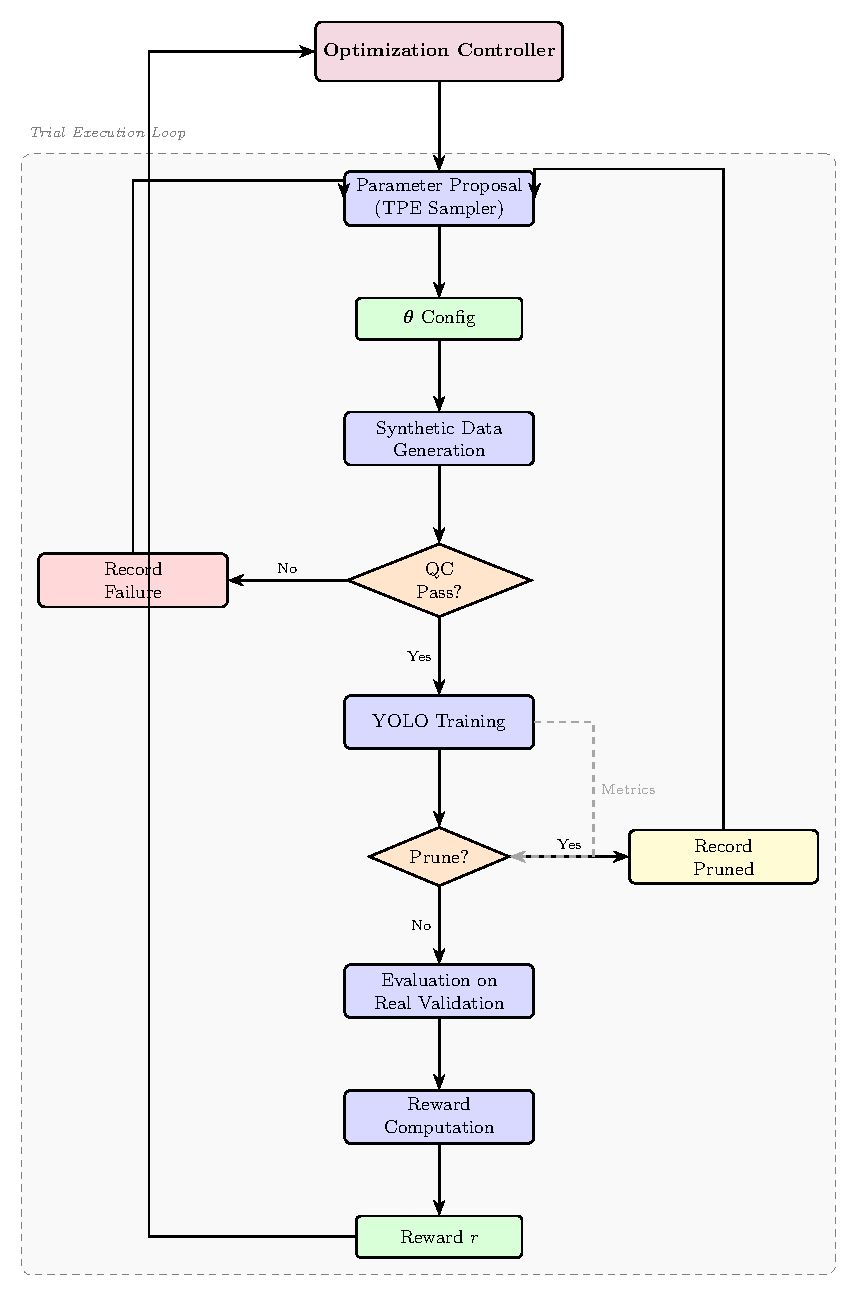
\includegraphics[width=0.75\textwidth]{figures/ch09_fig1_component_interaction.pdf}
\caption{Trial execution flowchart depicting the sequence of operations within each optimization trial. The Optimization Controller orchestrates parameter proposal through the TPE sampler, synthetic data generation, YOLO training with pruning evaluation, and reward computation. Decision diamonds indicate quality control and pruning checkpoints where trials may be terminated early. Dashed feedback paths show how intermediate training metrics inform pruning decisions and how reward signals guide subsequent parameter proposals.}
\label{fig:component_interaction}
\end{figure}

\subsection{System Architecture Diagram}

The following diagram illustrates the complete system architecture, depicting the six principal modules, their interconnections, and the flow of data and control signals throughout the optimization loop.

\begin{figure}[htbp]
\centering
\begin{tikzpicture}[
    node distance=1.8cm and 2.5cm,
    module/.style={rectangle, draw=black, thick, fill=blue!10, minimum width=4cm, minimum height=1.2cm, align=center, rounded corners=3pt},
    storage/.style={cylinder, draw=black, thick, fill=orange!20, shape border rotate=90, aspect=0.25, minimum width=2.5cm, minimum height=1cm, align=center},
    process/.style={rectangle, draw=black, thick, fill=green!10, minimum width=3.5cm, minimum height=1cm, align=center, rounded corners=3pt},
    arrow/.style={->, thick, >=stealth},
    dataarrow/.style={->, thick, >=stealth, color=blue!70},
    ctrlarrow/.style={->, thick, >=stealth, color=red!70, dashed}
]

% Main modules
\node[module] (optctrl) {\textbf{Optimization Controller}\\Optuna Study Manager};
\node[module, below=of optctrl] (synth) {\textbf{Synthetic Data Generation}\\Blender / Isaac Sim};
\node[module, below=of synth] (yolo) {\textbf{YOLO Training Module}\\Ultralytics Integration};
\node[module, right=3.5cm of yolo] (eval) {\textbf{Evaluation Module}\\Real Validation Assessment};
\node[module, right=3.5cm of synth] (reward) {\textbf{Reward Computation}\\Multi-Objective Aggregation};

% Storage components
\node[storage, left=2.5cm of optctrl] (studydb) {Study\\Database};
\node[storage, left=2.5cm of synth] (imgstore) {Image\\Storage};
\node[storage, left=2.5cm of yolo] (ckptstore) {Checkpoint\\Storage};
\node[storage, right=3.5cm of optctrl] (logstore) {Metrics\\Logs};

% Data flow arrows
\draw[dataarrow] (optctrl) -- node[left, font=\small] {Parameters} (synth);
\draw[dataarrow] (synth) -- node[left, font=\small] {Training Data} (yolo);
\draw[dataarrow] (yolo) -- node[below, font=\small] {Trained Model} (eval);
\draw[dataarrow] (eval) -- node[right, font=\small] {Metrics} (reward);
\draw[dataarrow] (reward) -- node[above, font=\small] {Reward Signal} (optctrl);

% Storage connections
\draw[arrow] (optctrl) -- (studydb);
\draw[arrow] (synth) -- (imgstore);
\draw[arrow] (yolo) -- (ckptstore);
\draw[arrow] (reward) -- (logstore);

% Control flow
\draw[ctrlarrow] (optctrl.south west) to[out=-150, in=150] node[left, font=\small, color=red!70] {Trial Control} (yolo.north west);

% Legend
\node[below=3.5cm of yolo, xshift=-2cm] (legend) {};
\draw[dataarrow] (legend) -- ++(1.5,0) node[right, font=\small] {Data Flow};
\draw[ctrlarrow] ([yshift=-0.5cm]legend) -- ++(1.5,0) node[right, font=\small] {Control Signal};

\end{tikzpicture}
\caption{System architecture diagram depicting the six principal modules and their interconnections. Blue solid arrows indicate data flow paths carrying parameters, images, models, and metrics. Red dashed arrows indicate control signals for trial management and early termination. Cylindrical nodes represent persistent storage components for study state, generated imagery, model checkpoints, and optimization logs.}
\label{fig:system_architecture}
\end{figure}

\subsection{Data Flow Through the System}

The data transformation pipeline begins with the Optimization Controller generating a parameter vector $\boldsymbol{\theta} \in \Theta$ specifying the complete configuration for synthetic data generation. This vector encompasses continuous parameters such as lighting intensity ranges and object scale bounds, discrete parameters such as the number of distractor objects per scene, and categorical parameters such as background environment selection. The parameter vector is serialized and transmitted to the Synthetic Data Generation Module along with metadata specifying the desired corpus size and output format.

The Synthetic Data Generation Module interprets the parameter vector to configure its internal randomization engine, procedurally generates the specified number of training images with corresponding annotations, performs quality assurance validation on the generated corpus, and writes the imagery and annotation files to designated storage locations. The module returns a manifest file specifying the paths to generated assets along with summary statistics describing the realized parameter distributions, enabling verification that the stochastic generation process produced outputs consistent with the specified configuration.

The YOLO Training Module consumes the generated corpus manifest to configure data loading pipelines, initializes model weights either from scratch or from a provided pretrained checkpoint, executes the training loop with periodic validation against a held-out synthetic validation subset, and persists model checkpoints at configurable intervals. Throughout training, the module exposes progress metrics through callback interfaces that enable the Optimization Controller to make pruning decisions based on intermediate performance indicators.

Upon training completion, the Evaluation Module loads the final model checkpoint and executes inference on the real-world validation set. The module computes comprehensive detection metrics including mean Average Precision at multiple Intersection over Union thresholds, per-class precision and recall statistics, and inference latency measurements. These metrics are aggregated into a structured evaluation report that is transmitted to the Reward Computation Module.

The Reward Computation Module transforms the multi-dimensional evaluation report into a scalar reward signal suitable for optimization algorithm consumption. This transformation involves normalization relative to historical performance distributions, application of weighting coefficients reflecting relative objective importance, detection and penalization of degenerate solutions, and optional temporal smoothing to reduce reward variance across stochastic training runs. The computed reward is returned to the Optimization Controller, completing the feedback loop and enabling informed proposal of subsequent parameter configurations.

\section{Synthetic Data Generation Module}
\label{sec:synth_data_module}

The Synthetic Data Generation Module bears responsibility for translating abstract parameter specifications into concrete training imagery that, despite its synthetic origin, induces detector representations capable of generalizing to real-world deployment scenarios. The module architecture supports multiple rendering backends through a unified abstraction layer, enabling practitioners to select generation engines appropriate to their specific domain requirements and computational resources.

\subsection{Blender and Isaac Sim Integration}

The module provides native integration with two primary rendering backends that collectively address the majority of synthetic data generation requirements encountered in practice. NVIDIA Isaac Sim, built upon the Omniverse platform, offers production-grade physics simulation, photorealistic path-traced rendering through the RTX renderer, and extensive libraries of simulation-ready assets with embedded semantic annotations. Isaac Sim integration is accomplished through the Omniverse Replicator API, which exposes programmatic control over scene composition, randomization parameters, and annotation generation through Python scripting interfaces.

Blender integration leverages the open-source three-dimensional creation suite's comprehensive Python API to achieve comparable functionality with reduced licensing complexity and hardware requirements. The Cycles rendering engine provides physically-based path tracing capable of photorealistic output, while the Eevee engine offers substantially faster rasterization-based rendering suitable for rapid prototyping and exploration phases of optimization campaigns. Blender's extensive material system supports physically-based rendering workflows with metallic, roughness, and normal mapping that accurately simulate real-world surface appearance under varied illumination conditions.

The backend abstraction layer defines a common interface through which the Optimization Controller interacts with either rendering engine without modification. This interface specifies methods for scene initialization, parameter application, frame rendering, and annotation export, enabling transparent backend substitution based on deployment requirements. The abstraction layer additionally provides automatic format conversion utilities that transform backend-specific annotation formats into the YOLO-compatible format required by downstream training pipelines.

\subsection{Parameter Space Definition}

The parameter space governing synthetic data generation encompasses multiple categories of configurable attributes, each contributing distinct aspects of visual variation to the generated corpus. The module maintains a hierarchical parameter specification that organizes individual parameters into semantically coherent groups while exposing the complete flattened vector to the optimization algorithm.

Object appearance parameters control the visual properties of target detection objects, encompassing texture selection from curated material libraries, color variation through hue-saturation-value perturbation, surface finish properties including metalness and roughness coefficients, and subsurface scattering parameters for translucent materials. These parameters collectively determine the feature distributions that trained detectors must recognize across the range of visual appearances exhibited by real-world objects.

Geometric variation parameters govern the spatial configuration of scene elements, including object position distributions within the scene volume, rotation distributions specifying allowable orientations, scale distributions defining size variation ranges, and aspect ratio perturbations that introduce controlled geometric distortion. Physics-based placement algorithms optionally simulate gravitational settling to achieve naturalistic object arrangements that avoid interpenetration artifacts.

Illumination parameters control the synthetic lighting environment, encompassing the number, positions, and intensities of point and area light sources, ambient illumination levels from environment maps, shadow characteristics determined by light source geometry, and color temperature variation spanning the range from warm tungsten to cool daylight illumination. High dynamic range environment maps provide image-based lighting that captures complex real-world illumination patterns including indirect reflections and color bleeding effects.

Camera parameters specify the virtual sensor configuration, including focal length determining field of view and perspective distortion characteristics, sensor dimensions affecting image resolution and aspect ratio, lens distortion coefficients modeling barrel and pincushion aberrations, and depth of field parameters when bokeh simulation is desired. Motion blur simulation parameters enable generation of imagery exhibiting the temporal integration artifacts characteristic of moving cameras or subjects.

Environmental parameters introduce scene-level variation through weather simulation including rain, fog, and snow effects, time-of-day variation affecting solar illumination angle and color, and atmospheric scattering models that introduce depth-dependent color shifts. Background variation parameters control the selection and configuration of scene backdrops ranging from solid colors through photographic backgrounds to fully three-dimensional environment geometry.

\begin{table}[htbp]
\centering
\caption{Synthetic Data Generation Parameter Categories and Typical Ranges}
\label{tab:parameter_space}
\begin{tabular}{p{3cm}p{4cm}p{3cm}p{4cm}}
\toprule
\textbf{Category} & \textbf{Parameter} & \textbf{Type} & \textbf{Typical Range} \\
\midrule
Object Appearance & Texture Library Index & Categorical & Domain-specific \\
 & Hue Variation & Continuous & $[-30, +30]$ degrees \\
 & Saturation Scale & Continuous & $[0.7, 1.3]$ \\
 & Metalness & Continuous & $[0.0, 1.0]$ \\
 & Roughness & Continuous & $[0.1, 0.9]$ \\
\addlinespace
Geometric & Position X/Y/Z & Continuous & Scene-dependent \\
 & Rotation Range & Continuous & $[0, 360]$ degrees \\
 & Scale Factor & Continuous & $[0.5, 2.0]$ \\
 & Object Count & Discrete & $[1, 20]$ \\
\addlinespace
Illumination & Light Count & Discrete & $[1, 8]$ \\
 & Intensity Range & Continuous & $[0.2, 5.0]$ \\
 & Color Temperature & Continuous & $[2700, 6500]$ Kelvin \\
 & Ambient Ratio & Continuous & $[0.1, 0.5]$ \\
\addlinespace
Camera & Focal Length & Continuous & $[24, 85]$ mm \\
 & Sensor Height & Continuous & Match deployment \\
 & Distortion k1 & Continuous & $[-0.3, 0.3]$ \\
\addlinespace
Environment & Fog Density & Continuous & $[0.0, 0.5]$ \\
 & Rain Intensity & Continuous & $[0.0, 1.0]$ \\
 & Time of Day & Continuous & $[0, 24]$ hours \\
\bottomrule
\end{tabular}
\end{table}

\subsection{Randomization Controller}

The Randomization Controller implements the stochastic sampling mechanisms that translate parameter specifications into concrete per-frame configurations. For each rendered frame, the Controller samples values from the distributions defined by the current parameter vector, applies these values to configure the scene state, and records the realized values in the frame metadata for subsequent analysis and debugging purposes.

The Controller supports multiple distribution families for continuous parameters, including uniform distributions for parameters with equally likely values throughout the specified range, truncated Gaussian distributions for parameters with preferred central values and diminishing probability toward range boundaries, and log-uniform distributions for parameters spanning multiple orders of magnitude such as lighting intensities. Discrete parameters employ categorical distributions with configurable probability masses for each allowable value.

Correlation structures among parameters are optionally specified through the parameter configuration, enabling the Controller to generate coherent multi-parameter variations that reflect real-world covariance patterns. For instance, outdoor illumination intensity and color temperature exhibit strong correlation in natural environments, with high intensities typically accompanying neutral color temperatures and low intensities accompanying warmer temperatures. The Controller implements Gaussian copula sampling to generate parameter vectors respecting specified correlation matrices while maintaining marginal distributions conforming to parameter-specific requirements.

The Controller additionally implements stratified sampling strategies that ensure systematic coverage of the parameter space across the generated corpus. Rather than independent sampling for each frame, stratified sampling partitions the parameter space into strata and generates equal numbers of samples from each stratum, reducing clustering artifacts and improving training data diversity for fixed corpus sizes. Latin hypercube sampling provides an efficient implementation of this strategy for high-dimensional parameter spaces.

\subsection{Annotation Generation in YOLO Format}

The annotation generation subsystem produces ground truth labels in the format expected by YOLO training pipelines, specifically normalized bounding box coordinates accompanied by integer class identifiers. For each rendered frame, the subsystem projects three-dimensional object bounding volumes into image coordinates, computes axis-aligned two-dimensional bounding rectangles enclosing the projected volumes, filters annotations for objects with insufficient visibility due to occlusion or frame boundary truncation, normalizes coordinates relative to image dimensions, and writes annotation files in the standard YOLO text format with one annotation per line.

Visibility computation accounts for occlusion by other scene objects through depth buffer analysis, determining the fraction of each object's projected area that remains unoccluded in the final rendered image. Objects with visibility below a configurable threshold are excluded from the annotation set to avoid training the detector on severely occluded instances that would be difficult to recognize even for human annotators. The visibility threshold represents a tunable parameter that balances training data completeness against annotation reliability.

The subsystem additionally generates segmentation masks and keypoint annotations when supported by the target detection architecture, enabling training of instance segmentation and pose estimation models alongside standard bounding box detectors. These extended annotations leverage the complete scene geometry information available in the synthetic environment to produce pixel-perfect ground truth that would require substantial manual effort to obtain for real-world imagery.

\subsection{Quality Assurance Checks}

The Quality Assurance subsystem validates generated imagery and annotations against configurable acceptance criteria, flagging or rejecting frames that fail to meet quality standards. Validation checks encompass both low-level image quality metrics and high-level semantic consistency requirements that collectively ensure the generated corpus provides effective training signal for downstream detector models.

Image quality validation verifies that rendered frames exhibit appropriate exposure levels without excessive clipping in highlight or shadow regions, sufficient contrast to enable feature extraction, absence of rendering artifacts such as fireflies in path-traced output, and spatial resolution adequate for detecting the smallest target objects. Frames failing quality thresholds trigger re-rendering with adjusted random seeds, ensuring that quality failures do not reduce the effective corpus size.

Annotation quality validation confirms that generated labels satisfy integrity constraints including non-empty annotation sets for frames containing target objects, bounding box coordinates within valid normalized ranges, class identifiers corresponding to defined object categories, and absence of degenerate boxes with zero area. The validation subsystem additionally computes corpus-level statistics including class balance ratios and object size distributions, flagging configurations that produce severely imbalanced or degenerate datasets.

\begin{figure}[htbp]
\centering
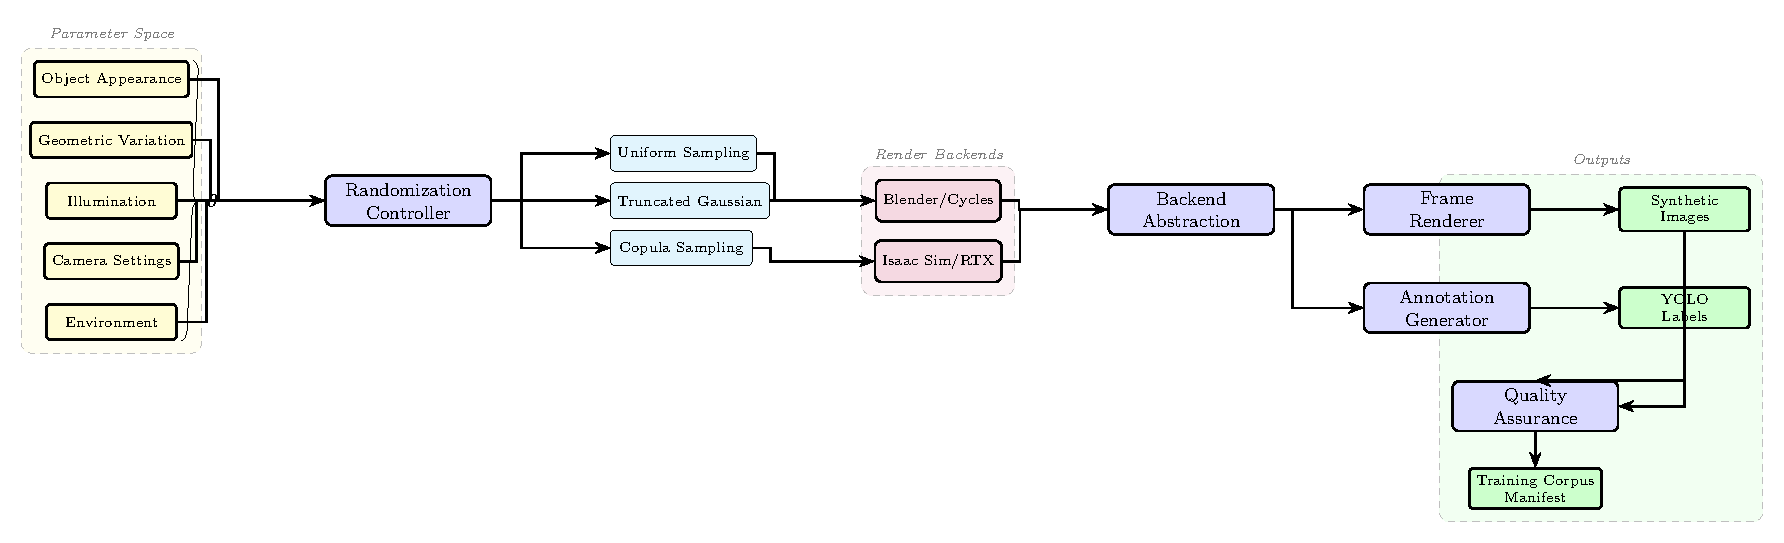
\includegraphics[width=\textwidth]{figures/ch09_fig2_synth_data_pipeline.pdf}
\caption{Synthetic data generation pipeline architecture. Parameter specifications flow from the parameter space through the Randomization Controller, which selects appropriate sampling strategies (uniform, truncated Gaussian, or copula-based) based on parameter characteristics. The rendering backend abstraction layer enables transparent switching between Blender and Isaac Sim engines. The pipeline produces synthetic images and YOLO-format annotations that undergo quality assurance validation before being assembled into the training corpus manifest.}
\label{fig:synth_data_pipeline}
\end{figure}

\section{YOLO Training Module}
\label{sec:yolo_training_module}

The YOLO Training Module encapsulates the complete neural network training workflow, providing a consistent interface through which the optimization system interacts with the underlying detection architecture regardless of the specific YOLO variant employed. The module architecture separates configuration management, training execution, and progress monitoring into distinct subsystems that collectively enable reliable automated training across diverse hardware configurations and experimental conditions.

\subsection{Ultralytics Integration}

The module achieves YOLO training capabilities through integration with the Ultralytics library, which provides production-grade implementations of YOLOv5, YOLOv8, and subsequent architecture revisions with consistent training APIs. Ultralytics integration is accomplished through programmatic invocation of the library's training entry points with configuration parameters derived from the optimization system's trial specifications.

The integration layer translates between the optimization system's internal parameter representation and the Ultralytics configuration format, mapping synthetic data generation parameters to data loader configurations, optimization hyperparameters to training settings, and architecture specifications to model constructors. This translation layer insulates the optimization system from implementation details of specific Ultralytics versions, enabling library upgrades without modification to the optimization codebase.

The integration additionally exposes Ultralytics callback interfaces to the optimization system, enabling registration of custom callbacks for progress monitoring, intermediate validation, and early termination. These callbacks receive training state information including current epoch, batch loss values, and validation metrics, transmitting this information to the Optimization Controller for pruning decisions and progress logging.

\subsection{Configuration Management}

The Configuration Management subsystem maintains hierarchical configuration structures that specify all parameters governing YOLO training execution. Configuration parameters are organized into categories encompassing model architecture selection, data augmentation strategies, optimization algorithm settings, learning rate scheduling, regularization techniques, and resource allocation directives.

Model architecture configuration specifies the YOLO variant and scale to employ, selecting among available backbone networks and head configurations. The configuration supports specification of pretrained weight paths for transfer learning scenarios, random weight initialization for training from scratch, and partial weight loading for architecture modification experiments. Input resolution configuration determines the spatial dimensions of images processed by the network, with implications for detection performance on small objects and computational resource requirements.

Data augmentation configuration controls the online augmentation pipeline applied to training images, specifying augmentation operations and their associated probability and magnitude parameters. Standard augmentations include geometric transformations such as scaling, rotation, and horizontal flipping, color space transformations such as hue, saturation, and brightness adjustment, and composite augmentations such as mosaic combining multiple training images into single inputs. Augmentation parameters may be fixed throughout optimization or included in the optimization parameter space for joint tuning with generation parameters.

Optimization configuration specifies the gradient descent algorithm, learning rate values and scheduling policies, batch size and gradient accumulation settings, and weight decay regularization strength. The subsystem supports SGD with momentum, Adam, and AdamW optimizers with configurable hyperparameters, along with learning rate schedulers including step decay, cosine annealing, and one-cycle policies.

\subsection{Checkpoint Handling}

The Checkpoint Handling subsystem manages model state persistence throughout training execution, enabling recovery from interruptions and provision of trained models to downstream evaluation. Checkpoints are persisted at configurable epoch intervals, with special handling for best-performing checkpoints determined by validation metrics and final-epoch checkpoints representing training completion.

The subsystem implements intelligent checkpoint retention policies that balance storage requirements against recovery capabilities. The rolling retention policy maintains only the most recent checkpoint along with the best-performing checkpoint, minimizing storage consumption while preserving the ability to resume from interruption and access peak-performance weights. The complete retention policy maintains all checkpoints throughout training, enabling detailed analysis of training dynamics at the cost of substantially increased storage requirements.

Checkpoint files include complete model state dictionaries, optimizer state enabling exact training resumption, epoch counters and learning rate scheduler states, and metadata describing the training configuration and data corpus. The standardized checkpoint format ensures compatibility with Ultralytics inference utilities and third-party analysis tools.

\subsection{Metrics Logging}

The Metrics Logging subsystem instruments training execution to capture comprehensive performance measurements enabling optimization algorithm feedback and experimental analysis. Logged metrics encompass training loss components, validation metrics, learning rate values, and timing measurements for each training epoch.

Training loss logging captures the individual loss components contributing to the total optimization objective, including objectness loss quantifying confidence calibration, classification loss measuring class prediction accuracy, and bounding box regression loss assessing localization precision. Component-level logging enables diagnosis of training dynamics and identification of loss terms dominating the optimization landscape.

Validation metrics logging records detector performance on held-out validation subsets at configurable intervals throughout training. Standard metrics include mean Average Precision at IoU threshold 0.50, mean Average Precision averaged across IoU thresholds from 0.50 to 0.95, and per-class Average Precision values enabling analysis of class-specific performance variation. These intermediate validation metrics provide the signals consumed by pruning algorithms for early termination decisions.

The logging subsystem integrates with standard experiment tracking platforms including TensorBoard, Weights and Biases, and MLflow, enabling visualization of training curves and comparison across optimization trials. Integration is accomplished through callback registration during training initialization, with the specific tracking platform selected through configuration parameters.

\subsection{GPU Resource Management}

The GPU Resource Management subsystem coordinates allocation of graphics processing resources across concurrent training workloads, ensuring efficient utilization while preventing resource contention that would degrade training throughput. The subsystem maintains awareness of available GPU devices, their memory capacities, and current utilization levels, informing scheduling decisions that maximize aggregate training throughput.

Device allocation policies specify how training workloads are assigned to available GPUs, ranging from exclusive allocation wherein each training process receives dedicated GPU resources through shared allocation wherein multiple lightweight processes time-slice a single device. The appropriate policy depends on model scale, batch size requirements, and the number of concurrent trials supported by the optimization configuration.

Memory management utilities monitor GPU memory utilization throughout training, implementing proactive batch size reduction when memory pressure exceeds configurable thresholds and gradient checkpointing activation when model scale approaches device memory limits. These adaptive mechanisms enable robust training execution across varied hardware configurations without manual tuning of memory-related hyperparameters.

Multi-GPU training support enables distribution of single training workloads across multiple devices through data parallelism, with automatic gradient synchronization and batch splitting managed by the underlying Ultralytics infrastructure. The Resource Management subsystem exposes configuration options for multi-GPU allocation and handles the additional complexity of coordinating distributed training with the checkpoint and metrics logging subsystems.

\section{Evaluation Module}
\label{sec:evaluation_module}

The Evaluation Module assesses trained detector performance against held-out real-world validation imagery, producing the performance metrics that ultimately determine optimization success. The module architecture addresses the statistical challenges inherent in evaluation with limited validation data, implementing robust estimation procedures that provide reliable performance signals despite validation set sizes that may be as small as fifty images.

\subsection{Real Validation Set Management}

The Validation Set Management subsystem maintains the real-world imagery corpus against which trained detectors are evaluated, ensuring consistent evaluation conditions across optimization trials while supporting validation set updates as additional real-world data becomes available. The validation set is isolated from synthetic training data through directory structure conventions and explicit path configuration, eliminating the possibility of data leakage that would inflate performance estimates.

The subsystem implements stratified subset selection utilities that construct evaluation batches balanced across object categories, ensuring that per-class performance metrics reflect evaluation on representative samples of each category. Stratification is accomplished through iterative selection that prioritizes images containing underrepresented categories until target class frequencies are achieved or the complete validation set is exhausted.

Validation set versioning enables tracking of evaluation corpus evolution across optimization campaigns, with checksum-based integrity verification ensuring that performance comparisons across trials employ identical evaluation data. The versioning system maintains association between trial results and validation set versions, enabling principled interpretation of historical results when validation sets are augmented with newly acquired real-world imagery.

Preprocessing pipelines applied to validation imagery are explicitly configured and version-controlled alongside the imagery itself, ensuring that evaluation conditions remain reproducible. Standard preprocessing operations include resolution normalization to match training input dimensions, color space conversion if required by the detection architecture, and optional test-time augmentation that evaluates each image under multiple transformations to improve prediction robustness.

\subsection{Bootstrap Confidence Computation}

The Bootstrap Confidence subsystem quantifies the statistical uncertainty associated with performance estimates derived from limited validation data, enabling principled comparison of detector performance across optimization trials and meaningful assessment of whether observed performance differences exceed expected sampling variation.

Bootstrap resampling constructs multiple pseudo-validation sets by sampling with replacement from the original validation corpus, computing detection metrics on each resampled set to generate an empirical distribution of performance estimates. Standard bootstrap procedures draw one thousand or more resamples, with the resampled metric distribution characterizing the statistical uncertainty attributable to validation set composition.

Confidence interval construction employs the percentile method, reporting the 2.5th and 97.5th percentiles of the bootstrap distribution as the bounds of a 95\% confidence interval. The bias-corrected and accelerated (BCa) bootstrap variant provides improved coverage properties when the sampling distribution exhibits skewness, as commonly occurs for bounded metrics such as precision and recall that approach their theoretical limits.

Statistical comparison utilities employ bootstrap hypothesis testing to determine whether performance differences between detector variants achieve statistical significance. The null hypothesis of equal population performance is evaluated by constructing a bootstrap distribution of performance differences and determining whether zero falls outside the resulting confidence interval. This procedure provides principled guidance for selecting among detector variants when observed performance differences are modest relative to sampling uncertainty.

\subsection{Class-Balanced mAP Calculation}

The Class-Balanced mAP subsystem computes mean Average Precision metrics that weight category contributions according to principled schemes reflecting application requirements, addressing the limitation of standard mAP computation wherein rare categories contribute minimally to aggregate scores despite their potential importance for deployment success.

Standard mAP computation averages per-class Average Precision values with uniform weights, implicitly prioritizing categories proportionally to their representation in the validation set. For imbalanced validation corpora where category frequencies diverge substantially from uniform distribution, this weighting scheme permits high aggregate scores while tolerating poor performance on underrepresented categories.

Class-balanced weighting assigns equal importance to each category regardless of validation set representation, computing the arithmetic mean of per-class Average Precision values. This scheme ensures that optimization pressure applies equally across categories, preventing the optimizer from discovering configurations that sacrifice rare-category performance to maximize aggregate metrics dominated by common categories.

Frequency-inverse weighting assigns category weights inversely proportional to validation set frequencies, amplifying the contribution of rare categories beyond equal weighting. This aggressive rebalancing scheme is appropriate when rare categories correspond to high-consequence detection targets whose reliable identification justifies disproportionate optimization effort.

The subsystem reports multiple mAP variants simultaneously, enabling practitioners to select the weighting scheme most appropriate for their application while monitoring alternative metrics for diagnostic purposes. Disagreement between uniformly-weighted and class-balanced metrics signals class-conditional performance variation that warrants investigation regardless of the primary optimization objective.

\subsection{Result Caching and History}

The Result Caching subsystem maintains persistent records of evaluation results across optimization campaigns, enabling historical analysis, reproducibility verification, and warm-starting of subsequent optimization runs from prior accumulated knowledge. The caching architecture separates ephemeral computation state from durable result records, ensuring that evaluation history survives system restarts and infrastructure changes.

The caching database records complete trial specifications including synthetic data generation parameters, training hyperparameters, random seeds, and software version identifiers alongside evaluation results encompassing all computed metrics and their bootstrap confidence intervals. This comprehensive recording enables post-hoc analysis of parameter-performance relationships, identification of promising parameter regions for focused exploration, and diagnosis of optimization pathologies.

Cache invalidation policies specify conditions under which cached results are discarded and recomputation triggered, addressing scenarios where cached results no longer reflect current system behavior. Invalidation triggers include validation set modifications, evaluation procedure changes, and detection of hardware-dependent result variation. Conservative invalidation policies that preserve cache entries across minor system changes maximize the value of accumulated evaluation history while accepting the risk of stale results under certain edge conditions.

History visualization utilities generate summary plots depicting optimization progress over trial sequences, parameter importance rankings derived from cached results, and performance-parameter scatter plots illuminating the optimization landscape structure. These visualizations support interactive exploration of optimization campaigns, informing parameter space refinement and identification of convergence to local optima.

\section{Optimization Controller}
\label{sec:optimization_controller}

The Optimization Controller implements the Bayesian optimization algorithm that proposes parameter configurations, manages trial execution, and maintains optimization state across potentially long-running campaigns. The Controller architecture employs the Optuna framework as its optimization backend, leveraging Optuna's sophisticated sampling algorithms, pruning mechanisms, and distributed execution capabilities while providing application-specific extensions for synthetic data optimization.

\subsection{Optuna Study Configuration}

Study configuration specifies the high-level structure of the optimization problem including the optimization direction, parameter space definition, and study persistence settings. The optimization direction indicates whether the objective should be maximized or minimized, with mAP optimization specifying maximization while loss-based objectives would specify minimization.

The parameter space definition enumerates all tunable parameters along with their types and domains, constructed from the union of synthetic data generation parameters, training hyperparameters, and optionally augmentation parameters. Continuous parameters specify lower and upper bounds along with optional distribution hints that inform the sampling algorithm. Discrete parameters enumerate allowable values with optional ordering information. Categorical parameters specify the set of allowable string or integer identifiers without implied ordering.

Study persistence configuration specifies the storage backend maintaining optimization state across Controller invocations. SQLite storage provides simple single-file persistence suitable for single-machine optimization campaigns. PostgreSQL storage enables distributed optimization with multiple workers proposing and evaluating trials concurrently while maintaining consistent study state. Redis storage provides in-memory persistence with optional durability, offering reduced latency for high-frequency trial operations at the cost of increased infrastructure complexity.

\begin{table}[htbp]
\centering
\caption{Optuna Study Configuration Parameters}
\label{tab:optuna_config}
\begin{tabular}{p{3.5cm}p{3cm}p{6.5cm}}
\toprule
\textbf{Parameter} & \textbf{Default Value} & \textbf{Description} \\
\midrule
study\_name & Required & Unique identifier for the optimization study \\
direction & maximize & Optimization direction for the primary objective \\
storage & sqlite:///study.db & Database URL for study persistence \\
load\_if\_exists & True & Resume existing study if present \\
n\_startup\_trials & 10 & Random trials before TPE sampling begins \\
n\_ei\_candidates & 24 & Candidates evaluated for expected improvement \\
multivariate & True & Model parameter correlations in TPE \\
\bottomrule
\end{tabular}
\end{table}

\subsection{TPE Sampler Setup}

The Tree-structured Parzen Estimator sampler implements the parameter proposal mechanism that balances exploration of unvisited parameter regions against exploitation of promising regions identified through prior evaluations. TPE constructs separate density models over parameter configurations yielding above-threshold and below-threshold objective values, proposing configurations that maximize the ratio of above-threshold to below-threshold density.

Startup trial configuration specifies the number of initial trials sampled uniformly at random before TPE modeling commences. Sufficient startup trials ensure that the TPE model receives diverse observations spanning the parameter space, preventing premature convergence to local optima based on unrepresentative initial samples. The recommended startup count scales with parameter dimensionality, with ten trials providing adequate coverage for optimization problems with fewer than fifteen parameters.

Candidate evaluation count determines the number of parameter configurations evaluated during acquisition function optimization, with the highest-scoring candidate selected for the next trial. Larger candidate counts provide more thorough acquisition function optimization at the cost of increased computational overhead, with twenty-four candidates representing a reasonable balance for typical optimization problems.

Multivariate modeling enables the TPE sampler to capture correlations among parameters, constructing joint density models rather than independent per-parameter models. Multivariate modeling improves sample efficiency when parameters interact strongly, as commonly occurs in synthetic data generation where lighting and material parameters jointly determine rendered appearance. The computational overhead of multivariate modeling scales polynomially with parameter count, potentially necessitating independent modeling for high-dimensional problems.

\subsection{Hyperband Pruner Configuration}

The Hyperband pruner implements early termination of unpromising trials based on intermediate performance measurements, substantially reducing computational expenditure by abandoning trials whose trajectory indicates low probability of achieving competitive final performance. Hyperband extends successive halving to automatically determine appropriate resource allocation without requiring manual specification of the exploration-exploitation tradeoff.

Minimum resource configuration specifies the earliest training stage at which pruning decisions are considered, preventing premature termination based on unreliable early-training metrics. For YOLO training, minimum resource is typically specified in epochs, with values between five and fifteen epochs ensuring that pruning decisions reflect model behavior beyond random initialization.

Maximum resource configuration specifies the full training budget assigned to unpruned trials that survive all intermediate evaluations. The ratio of maximum to minimum resource determines the reduction factor applied at each pruning stage, with trials surviving each stage receiving multiplicatively increased resources until reaching the maximum allocation.

Reduction factor determines the fraction of trials promoted at each successive halving stage, with larger reduction factors providing more aggressive pruning at the cost of increased risk of discarding trials that would ultimately achieve strong performance. The default reduction factor of three retains one-third of trials at each stage, providing a reasonable balance between computational savings and optimization reliability.

\begin{table}[htbp]
\centering
\caption{Hyperband Pruner Configuration Parameters}
\label{tab:hyperband_config}
\begin{tabular}{p{3.5cm}p{3cm}p{6.5cm}}
\toprule
\textbf{Parameter} & \textbf{Default Value} & \textbf{Description} \\
\midrule
min\_resource & 1 & Minimum budget before pruning eligibility \\
max\_resource & auto & Maximum budget for complete trials \\
reduction\_factor & 3 & Fraction of trials surviving each stage \\
bootstrap\_count & 0 & Startup trials before pruning begins \\
\bottomrule
\end{tabular}
\end{table}

\subsection{Trial Management}

The Trial Management subsystem coordinates the lifecycle of individual optimization trials from parameter proposal through evaluation completion, handling both successful completions and various failure modes that may interrupt trial execution. Trial state transitions follow a well-defined state machine with states for running, complete, pruned, and failed trials.

Trial initialization allocates a unique trial identifier, samples parameter values from the configured sampler, records the proposed configuration to persistent storage, and transitions the trial to running state. The parameter sampling process queries the sampler with the current trial handle, enabling the sampler to access the complete optimization history when generating proposals.

Trial execution invokes the synthetic data generation, training, and evaluation pipeline with the proposed parameters, reporting intermediate metrics to the pruner at configurable intervals. Intermediate reporting enables pruning decisions during training execution, avoiding the computational waste of completing training runs whose intermediate performance indicates poor final outcomes.

Trial completion records final evaluation metrics to the study database and transitions the trial to completed state. The completion handler additionally updates sampler state with the new observation, enabling subsequent proposals to benefit from the accumulated evaluation history. Failed trials resulting from infrastructure errors or invalid parameter combinations transition to failed state with recorded failure reasons, excluding their results from sampler modeling while preserving diagnostic information.

\subsection{Database Persistence}

The Database Persistence subsystem maintains durable records of optimization state enabling recovery from system failures, analysis of optimization history, and coordination among distributed optimization workers. The persistence architecture employs relational database storage with a schema capturing studies, trials, parameter values, and intermediate results.

The study table maintains high-level study metadata including study names, creation timestamps, optimization directions, and study-level configuration. The trial table records individual trials with foreign key references to parent studies, capturing trial states, objective values, and completion timestamps. The parameter value table stores parameter configurations as key-value pairs with trial foreign keys, enabling reconstruction of complete parameter vectors for any historical trial.

Transaction semantics ensure atomic updates to study state, preventing inconsistent views when multiple workers access shared studies concurrently. Isolation levels balance consistency requirements against throughput, with serializable isolation appropriate for small-scale optimization and read-committed isolation enabling higher concurrency for large-scale distributed campaigns.

Backup and recovery procedures protect against data loss from database corruption or infrastructure failures. Scheduled backup jobs export study state to archival storage, with point-in-time recovery capabilities enabling restoration to any historical state within the backup retention window. Recovery procedures verify database integrity after restoration, recomputing derived state that may have diverged during the failure interval.

\begin{figure}[htbp]
\centering
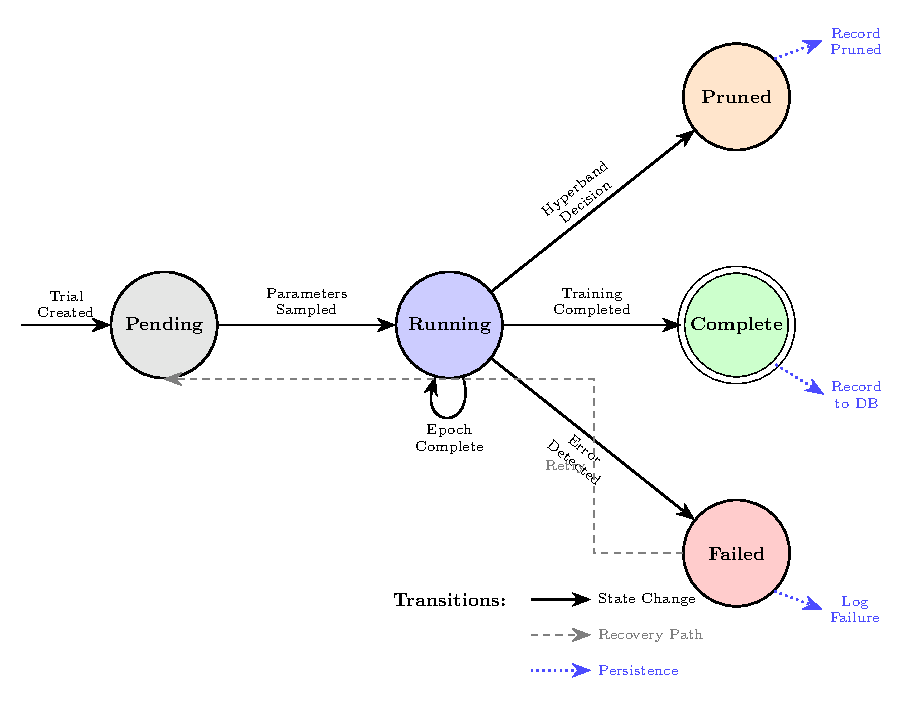
\includegraphics[width=0.85\textwidth]{figures/ch09_fig4_trial_state_machine.pdf}
\caption{Trial lifecycle state machine depicting the possible states and transitions for optimization trials. Trials begin in the Pending state upon creation, transition to Running when parameters are sampled, and terminate in one of three states: Complete (successful training and evaluation), Pruned (early termination by Hyperband), or Failed (error during execution). The self-loop on Running represents epoch completions during training. Dashed arrows indicate recovery paths for failed trials that may be retried, while dotted arrows show database persistence operations for each terminal state.}
\label{fig:trial_state_machine}
\end{figure}

\section{Reward Computation Module}
\label{sec:reward_computation}

The Reward Computation Module transforms multi-dimensional evaluation metrics into scalar reward signals suitable for consumption by the optimization algorithm, implementing the objective function that implicitly defines which parameter configurations the optimizer will prefer. The module architecture supports flexible reward formulations ranging from simple single-metric objectives through complex composite functions balancing multiple competing concerns.

\subsection{Component Calculation}

The Component Calculation subsystem computes the individual reward components that may contribute to the aggregate objective, each component capturing a distinct aspect of detector performance relevant to deployment success. Standard components include detection accuracy metrics, computational efficiency measurements, and domain adaptation indicators.

Detection accuracy components derive directly from evaluation metrics computed by the Evaluation Module, typically employing mean Average Precision at standard IoU thresholds as the primary performance indicator. Per-class Average Precision values may contribute as auxiliary components when class-specific performance requirements constrain the optimization. Precision-recall tradeoff points at fixed confidence thresholds provide alternative accuracy characterizations when detection operating points are predetermined by application requirements.

Computational efficiency components quantify the resource consumption associated with detector inference, enabling optimization that balances accuracy against deployment constraints. Inference latency measurements capture wall-clock time required for processing individual images, with the specific measurement methodology matching deployment hardware to ensure transferable efficiency estimates. Model complexity metrics including parameter counts and floating-point operation counts provide hardware-independent efficiency proxies when deployment hardware differs from evaluation infrastructure.

Domain adaptation components quantify the apparent domain shift between synthetic training data and real validation imagery, providing optimization signal that encourages generation of synthetic data whose distribution aligns with real-world conditions. Feature distribution divergence metrics compare intermediate network activations on synthetic and real images, with lower divergence indicating better domain alignment. Classifier uncertainty metrics aggregate prediction confidence statistics that may reveal distribution shift even when detection accuracy remains acceptable.

\subsection{Normalization and Smoothing}

The Normalization subsystem transforms raw reward components into standardized scales suitable for aggregation, addressing the scale incompatibilities that arise when combining metrics with different natural units and ranges. Normalization ensures that component weighting coefficients operate on comparable scales, enabling intuitive specification of relative component importance.

Range normalization maps component values to the unit interval through linear transformation based on observed or specified minimum and maximum values. Observed range normalization computes bounds from historical component distributions, automatically adapting to the realized performance range as optimization progresses. Specified range normalization employs fixed bounds derived from domain knowledge, providing stable normalization throughout optimization but requiring accurate bound specification to avoid clipped values.

Z-score normalization transforms components to zero mean and unit variance based on historical distributions, producing unbounded normalized values whose magnitudes indicate deviation from typical performance. Z-score normalization automatically adapts to performance distributions without requiring bound specification, but produces less interpretable normalized values and may exhibit instability during early optimization when historical distributions are poorly characterized.

Temporal smoothing reduces reward variance arising from stochastic training and evaluation procedures, providing more stable optimization signal at the cost of delayed response to genuine performance changes. Exponential moving average smoothing computes weighted combinations of current and historical rewards, with the smoothing coefficient balancing variance reduction against response latency. Windowed averaging computes unweighted means over recent trial sequences, providing uniform historical weighting but exhibiting step discontinuities as trials exit the averaging window.

\subsection{Degenerate Solution Detection}

The Degenerate Solution Detection subsystem identifies parameter configurations that achieve superficially strong reward values through pathological behaviors rather than genuine detection capability, flagging or penalizing such configurations to prevent optimization convergence to undesirable solutions.

Empty prediction detection identifies trials where trained detectors produce no predictions on validation imagery, a degenerate behavior that achieves perfect precision through prediction abstention. The detection mechanism examines prediction counts across validation images, flagging trials with prediction counts below configurable thresholds relative to annotation counts. Detected trials receive substantial reward penalties that ensure subsequent proposals avoid the degenerate parameter region.

Class collapse detection identifies trials where trained detectors predict only a single class regardless of actual object categories, achieving high accuracy on majority classes while failing completely on minority categories. The detection mechanism computes prediction class entropy across validation imagery, flagging trials with entropy below thresholds indicating collapsed prediction distributions. Adaptive thresholds account for natural class imbalance in validation annotations, distinguishing genuine class collapse from appropriate majority-class bias.

Confidence collapse detection identifies trials where trained detectors assign extreme confidence values to all predictions, eliminating the nuanced confidence calibration required for effective precision-recall tradeoff navigation. The detection mechanism computes confidence value variance across predictions, flagging trials with variance below thresholds indicating collapsed confidence distributions. Detected trials typically indicate training pathologies requiring hyperparameter adjustment rather than generation parameter modification.

\subsection{Logging and Monitoring}

The Logging subsystem instruments reward computation to capture comprehensive diagnostic information enabling analysis of optimization dynamics and identification of reward formulation issues. Logged information encompasses raw component values, normalized component values, aggregate rewards, and degenerate detection flags for each evaluated trial.

Component-level logging enables post-hoc analysis of which reward components drive optimization progress, informing refinement of component weights and identification of redundant or conflicting components. Temporal analysis of component trajectories reveals optimization phases where different components dominate, supporting adaptive weighting schemes that emphasize different objectives at different optimization stages.

Monitoring dashboards aggregate logging output into real-time visualizations depicting optimization progress, reward distributions, and component contributions. Standard dashboard panels include reward trajectory plots showing aggregate and component rewards over trial sequences, parameter importance rankings derived from trial comparisons, and degenerate detection alerts highlighting trials flagged for pathological behaviors.

Alert systems notify operators of optimization events requiring attention, including extended periods without reward improvement suggesting convergence or stagnation, elevated degenerate detection rates suggesting systematic parameter space issues, and infrastructure errors interrupting trial execution. Alert routing configurations specify notification channels and escalation policies appropriate to organizational requirements.

\section{Implementation Roadmap}
\label{sec:implementation_roadmap}

The implementation roadmap organizes system development into sequential phases that progressively construct operational optimization capabilities while validating assumptions and calibrating configuration parameters. The phased approach enables early detection of architectural issues, provides checkpoints for stakeholder review, and reduces risk relative to monolithic development approaches that defer integration until project completion.

\subsection{Phase 1: Infrastructure Setup}

The infrastructure setup phase establishes the foundational computational environment, software dependencies, and data management systems required by subsequent phases. Phase completion criteria include successful execution of isolated module tests and establishment of monitoring and logging infrastructure.

Computational infrastructure provisioning encompasses GPU server allocation, storage system configuration, and network connectivity establishment. GPU servers require CUDA-capable devices with sufficient memory for YOLO training at target input resolutions, with memory requirements scaling with model architecture and batch size selections. Storage systems require sufficient capacity for generated synthetic imagery, model checkpoints, and optimization databases, with typical campaigns requiring several hundred gigabytes of persistent storage.

Software dependency installation establishes Python environments with required libraries including PyTorch for neural network computation, Ultralytics for YOLO training, Optuna for optimization, and rendering backend libraries appropriate to the selected generation engine. Dependency version pinning ensures reproducible environments across development and deployment systems, with version specifications recorded in requirements manifests.

Data management infrastructure configuration establishes directory structures for synthetic imagery, validation sets, checkpoints, and logs, along with backup procedures and retention policies appropriate to operational requirements. Access control configuration restricts system access to authorized personnel while enabling automated processes to access required resources.

\subsection{Phase 2: Calibration Runs}

The calibration phase executes preliminary optimization campaigns with reduced computational budgets to validate system integration, characterize baseline performance levels, and calibrate configuration parameters. Phase completion criteria include successful end-to-end execution of optimization loops and establishment of baseline performance benchmarks.

Integration validation executes complete optimization trials to verify correct interaction among system modules, identifying interface mismatches, data format inconsistencies, and timing dependencies that impede reliable execution. Integration issues discovered during calibration are resolved before proceeding to computationally expensive main optimization campaigns.

Baseline performance characterization evaluates detector performance under default generation parameters, establishing the performance level against which optimization improvements are measured. Baseline evaluation additionally characterizes performance variance arising from stochastic training, informing confidence interval computation and convergence detection thresholds.

Configuration calibration determines appropriate values for system parameters not subject to optimization, including pruning thresholds, logging frequencies, and checkpoint intervals. Calibration experiments evaluate system behavior under candidate parameter values, selecting values that balance computational efficiency against operational reliability.

\subsection{Phase 3: Main Optimization}

The main optimization phase executes full-scale optimization campaigns with production computational budgets, discovering parameter configurations that maximize detector performance on real-world validation imagery. Phase completion criteria include convergence to stable performance levels and documentation of discovered optimal configurations.

Optimization campaign execution instantiates the Optimization Controller with production configuration and monitors execution progress through logging and dashboard infrastructure. Operator intervention addresses infrastructure issues and adjusts configuration parameters if optimization dynamics indicate suboptimal settings.

Convergence monitoring tracks performance improvement over trial sequences, identifying plateau regions indicating local optima or global convergence. Convergence detection triggers human review of optimization results, determining whether discovered configurations achieve acceptable performance or whether additional optimization effort is warranted.

Result documentation records optimal parameter configurations, achieved performance levels, and optimization trajectories for subsequent analysis and reporting. Documentation includes sufficient detail to enable reproduction of optimization campaigns and interpretation of results by stakeholders unfamiliar with system internals.

\subsection{Phase 4: Final Validation}

The final validation phase subjects discovered optimal configurations to rigorous evaluation establishing confidence in deployment readiness. Phase completion criteria include statistical validation of performance claims and documentation suitable for deployment approval processes.

Extended evaluation expands assessment beyond the validation set employed during optimization, evaluating detector performance on held-out test imagery and optionally on imagery from related domains. Extended evaluation guards against overfitting to validation set idiosyncrasies and characterizes generalization capabilities relevant to deployment success.

Statistical validation applies hypothesis testing procedures to compare optimal configurations against baseline configurations and alternative optimization approaches, establishing statistically significant performance improvements. Validation reports document achieved confidence levels and characterize remaining uncertainty in performance estimates.

Deployment documentation produces comprehensive records of optimal configurations, performance characteristics, and operational requirements suitable for handoff to deployment teams. Documentation includes configuration files, trained model weights, and operational procedures enabling deployment teams to instantiate operational detectors without requiring optimization expertise.

\begin{table}[htbp]
\centering
\caption{Implementation Roadmap Timeline and Milestones}
\label{tab:implementation_timeline}
\begin{tabular}{p{2cm}p{3.5cm}p{3cm}p{5cm}}
\toprule
\textbf{Phase} & \textbf{Duration} & \textbf{Compute Budget} & \textbf{Key Deliverables} \\
\midrule
Phase 1 & 1--2 weeks & Minimal & Configured infrastructure, module tests passing, monitoring operational \\
\addlinespace
Phase 2 & 1--2 weeks & 10--20 trials & Integration validated, baseline performance characterized, parameters calibrated \\
\addlinespace
Phase 3 & 2--4 weeks & 50--100 trials & Converged optimization, optimal configurations documented, performance targets achieved \\
\addlinespace
Phase 4 & 1--2 weeks & 5--10 trials & Statistical validation complete, deployment documentation delivered, approval obtained \\
\bottomrule
\end{tabular}
\end{table}

\begin{figure}[htbp]
\centering
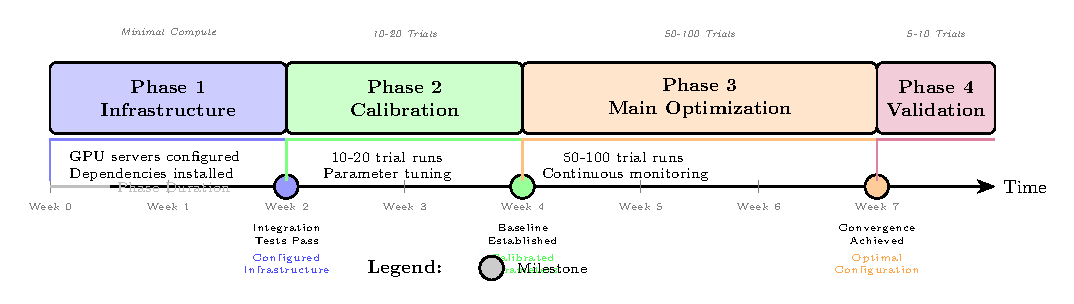
\includegraphics[width=\textwidth]{figures/ch09_fig3_implementation_roadmap.pdf}
\caption{Implementation roadmap timeline visualization showing the four phases of system deployment. Each phase is represented with its duration, computational budget, and key milestones. Phase 1 (Infrastructure) establishes the computational environment with minimal compute requirements. Phase 2 (Calibration) runs initial trials to establish baselines. Phase 3 (Main Optimization) executes the primary optimization campaign with 50--100 trials. Phase 4 (Validation) performs statistical validation and prepares deployment documentation. Milestones mark the completion of each phase with specific deliverables.}
\label{fig:implementation_roadmap}
\end{figure}

\section{Practical Considerations}
\label{sec:practical_considerations}

Production deployment of optimization systems encounters practical challenges extending beyond algorithmic correctness, requiring engineering solutions that ensure reliable operation under real-world conditions. This section addresses common operational challenges and presents strategies for robust system operation.

\subsection{Checkpointing and Recovery}

Robust checkpointing strategies ensure that system failures result in bounded work loss rather than complete campaign restart. The checkpointing architecture captures complete system state at configurable intervals, enabling recovery to any checkpointed state with guaranteed consistency.

Study-level checkpointing persists Optuna study state to durable storage, capturing completed trial results, pending trial states, and sampler internal state. Database storage backends provide automatic checkpointing through transaction logging, while file-based storage requires explicit checkpoint operations. Recovery from study checkpoints restores complete optimization history, enabling continued optimization from the last persisted state.

Model-level checkpointing persists YOLO training state at epoch boundaries, capturing model weights, optimizer state, and training progress. Checkpoint frequency balances recovery granularity against storage and I/O overhead, with per-epoch checkpointing appropriate for production campaigns where recovery time exceeds epoch duration. Recovery from model checkpoints resumes training from the checkpointed epoch, avoiding repetition of completed training work.

Data-level checkpointing records generated synthetic imagery and annotations to persistent storage, enabling training resumption without regeneration. Corpus generation typically dominates checkpoint storage requirements, motivating retention policies that balance storage consumption against regeneration cost. Checksums enable verification of corpus integrity after recovery, detecting corruption that would contaminate subsequent training.

\subsection{Handling Failed Training Runs}

Training failures arising from numerical instabilities, resource exhaustion, or software errors require graceful handling that preserves optimization progress while avoiding systematic bias from failure patterns. The failure handling strategy distinguishes recoverable failures warranting retry from persistent failures requiring parameter adjustment.

Automatic retry policies specify the maximum number of retry attempts before declaring trial failure, along with backoff intervals between attempts that may permit transient resource contention to resolve. Retry attempts optionally modify training configuration through batch size reduction, learning rate adjustment, or random seed changes that may circumvent failure-inducing conditions.

Failure penalty assignment determines the objective value recorded for persistently failed trials, influencing subsequent sampling behavior. Pessimistic penalties assign values worse than any observed successful trial, strongly discouraging sampling in failure-inducing parameter regions. Neutral penalties exclude failed trials from sampler modeling, preventing failure patterns from biasing proposals while forgoing the information that failures provide about parameter space structure.

Failure pattern analysis examines failure rates across parameter regions, identifying systematic failure modes that warrant parameter space constraints or configuration adjustments. Persistent failures concentrated in specific parameter subspaces may indicate incompatible generation parameters, overly aggressive training configurations, or infrastructure limitations requiring architectural revision.

\subsection{Warm-Starting from Prior Knowledge}

Warm-starting strategies accelerate optimization convergence by initializing from prior knowledge accumulated through previous campaigns, domain expertise, or related optimization problems. Effective warm-starting can reduce iteration counts by thirty to fifty percent compared to cold-starting, substantially reducing computational expenditure.

Historical trial injection populates new studies with results from previous optimization campaigns, providing the sampler with prior observations that inform initial proposals. Injected trials must be compatible with current parameter space definitions, potentially requiring transformation when parameter spaces differ between campaigns. Compatibility verification prevents injection of incompatible trials that would corrupt sampler modeling.

Expert configuration seeding initializes optimization with parameter configurations derived from domain expertise or published best practices, ensuring that known-good configurations receive evaluation regardless of sampler proposals. Seeded configurations are enqueued as pending trials that execute before sampler-generated proposals, providing immediate evaluation of expert knowledge.

Transfer learning from related problems leverages optimization results from similar but distinct domains, potentially informing proposals even when target domain differs from source domain. Transfer effectiveness depends on domain similarity, with conservative transfer strategies that downweight source observations appropriate when domain relationships are uncertain.

\subsection{Logging and Visualization}

Comprehensive logging enables retrospective analysis of optimization behavior, supporting both immediate debugging and long-term system improvement. The logging architecture captures structured records at multiple granularities from individual function invocations through complete optimization campaigns.

Structured logging employs standardized formats that enable automated parsing and aggregation, with JSON formatting providing flexibility for heterogeneous log entries. Log records include timestamps, log levels, component identifiers, and structured payloads capturing event-specific information. Centralized log aggregation enables correlation analysis across distributed system components.

Real-time visualization presents optimization progress through continuously-updated dashboards displaying key metrics and system status. Standard dashboard elements include objective value trajectories, parameter distributions, trial status summaries, and resource utilization indicators. Interactive visualization enables drill-down from aggregate views to individual trial details.

Post-hoc analysis tools process logged data to extract insights informing system improvement, including parameter importance analysis identifying high-impact parameters, convergence analysis characterizing optimization efficiency, and failure analysis identifying systematic issues requiring architectural attention.

\subsection{Debugging Strategies}

Systematic debugging strategies accelerate issue resolution when optimization behavior deviates from expectations, whether through failure to improve, convergence to suboptimal configurations, or erratic optimization dynamics. Effective debugging leverages comprehensive logging to localize issues and reproduce failures in controlled conditions.

Reproducibility enforcement ensures that debugging investigations can recreate observed behaviors, requiring complete capture of random seeds, software versions, and environmental conditions. Reproducibility verification confirms that recorded conditions suffice to recreate behavior before commencing investigation.

Isolation strategies narrow issue scope by disabling or mocking system components to determine which module contributes to observed misbehavior. Progressive isolation begins with coarse component boundaries and proceeds to finer granularities as investigation narrows the likely issue location.

Reference implementations provide known-correct behavior against which production system output can be compared, identifying discrepancies that localize issues. Reference implementations sacrifice efficiency for clarity and correctness, enabling verification without requiring comprehension of production optimization.

\section{Recommended Tools and Libraries}
\label{sec:recommended_tools}

Tool selection significantly impacts implementation effort, operational reliability, and extensibility to future requirements. This section presents recommendations based on evaluation of available options against the specific requirements of synthetic data optimization for object detection.

\subsection{Optuna for Optimization}

Optuna provides the optimization algorithm implementation recommended for synthetic data parameter tuning, offering mature implementations of Tree-structured Parzen Estimation, Hyperband pruning, and distributed optimization coordination with minimal integration effort.

The TPE sampler implementation handles mixed parameter types including continuous, discrete, and categorical parameters with appropriate kernel density estimation for each type. Multivariate modeling captures parameter correlations that improve sample efficiency when parameters interact. Automatic handling of conditional parameters enables complex parameter space definitions with dependencies among parameters.

The pruning framework provides Hyperband and successive halving implementations that integrate seamlessly with training callbacks, enabling early termination decisions based on intermediate training metrics. Pruning configuration requires minimal hyperparameter specification, with sensible defaults appropriate for most optimization problems.

The distributed optimization capabilities enable parallel trial execution across multiple workers sharing study state through database storage backends. Worker coordination ensures consistent study state despite concurrent access, with transaction isolation preventing conflicts between simultaneous parameter proposals.

\subsection{Ultralytics for YOLO}

The Ultralytics library provides YOLO implementation recommended for detector training, offering production-grade implementations of contemporary YOLO architectures with consistent training and inference APIs.

Architecture support encompasses YOLOv5, YOLOv8, and subsequent architecture revisions, enabling architecture selection based on accuracy-efficiency tradeoffs appropriate to deployment requirements. Pretrained weights for standard architectures enable transfer learning that accelerates training convergence and improves final accuracy.

Training utilities implement contemporary training techniques including mosaic augmentation, automatic learning rate finding, and mixed-precision training that maximize accuracy within computational constraints. Export utilities produce optimized model formats for deployment including ONNX, TensorRT, and CoreML.

The callback system enables integration with external monitoring and control systems, providing hooks for training progress reporting, intermediate validation, and early termination. Callback-based integration preserves library upgrade compatibility by avoiding modifications to library internals.

\subsection{Blender and Isaac Sim for Generation}

Blender and NVIDIA Isaac Sim provide complementary synthetic data generation capabilities addressing different requirements along the flexibility-capability tradeoff.

Blender's open-source license eliminates licensing costs while providing comprehensive three-dimensional modeling, animation, and rendering capabilities through an extensive Python API. The Cycles renderer provides physically-based path tracing producing photorealistic output, while the Eevee renderer provides faster rasterization-based rendering suitable for rapid iteration. Community extensions provide domain-specific functionality for common synthetic data generation requirements.

Isaac Sim provides production-grade synthetic data generation integrated with NVIDIA's Omniverse platform, offering advanced physics simulation, photorealistic rendering through RTX acceleration, and extensive asset libraries with simulation-ready models. The Replicator API provides high-level abstractions for common generation tasks including randomization, annotation, and format conversion. Enterprise support provides assistance for production deployment requirements.

The backend abstraction layer enables use of either generation engine through consistent interfaces, with backend selection based on available hardware, licensing constraints, and domain-specific requirements. Hybrid approaches employing different backends for different generation tasks combine the strengths of each platform.

\subsection{Ray for Parallelization}

Ray provides distributed computing capabilities that enable parallel execution of optimization trials, generation processes, and training workloads across heterogeneous computational resources.

The task-based programming model enables straightforward parallelization of independent operations without explicit coordination logic, with the Ray runtime handling task scheduling, data movement, and failure recovery. Task dependencies expressed through object references enable automatic pipeline execution when dependent tasks produce required inputs.

The actor-based programming model enables stateful computations that maintain context across method invocations, appropriate for generation engines and training processes that benefit from persistent state. Actor lifecycle management handles initialization, checkpointing, and recovery automatically.

Integration with Optuna enables distributed optimization with Ray-based parallel trial execution, scaling optimization throughput linearly with available computational resources while maintaining optimization algorithm correctness through centralized study state management.

\begin{table}[htbp]
\centering
\caption{Comparison of Recommended Tools and Alternatives}
\label{tab:tool_comparison}
\begin{tabular}{p{2.5cm}p{3.5cm}p{3.5cm}p{4cm}}
\toprule
\textbf{Category} & \textbf{Recommended} & \textbf{Alternatives} & \textbf{Selection Rationale} \\
\midrule
Optimization & Optuna & Hyperopt, BoTorch, SMAC & Mature TPE/Hyperband, excellent distributed support, active development \\
\addlinespace
Detection & Ultralytics & Detectron2, MMDetection & Production-ready YOLO, consistent API, comprehensive documentation \\
\addlinespace
Generation & Blender + Isaac Sim & Unity Perception, Unreal Engine & Flexibility + capability coverage, strong Python integration \\
\addlinespace
Parallelization & Ray & Dask, multiprocessing & Unified task/actor model, Optuna integration, enterprise support \\
\addlinespace
Logging & TensorBoard + W\&B & MLflow, Neptune & Wide adoption, real-time visualization, experiment comparison \\
\addlinespace
Storage & PostgreSQL & SQLite, MySQL & Concurrent access, transaction support, mature tooling \\
\bottomrule
\end{tabular}
\end{table}

\section{Main Optimization Loop Algorithm}
\label{sec:main_algorithm}

The main optimization loop algorithm integrates the modules described in preceding sections into a complete procedure for discovering optimal synthetic data generation parameters. The algorithm implements the BOHB optimization strategy with multi-fidelity evaluation through Hyperband pruning.

\begin{algorithm}[htbp]
\caption{Main Synthetic Data Optimization Loop}
\label{alg:main_optimization}
\begin{algorithmic}[1]
\Require Parameter space $\Theta$, validation set $\mathcal{V}$, computational budget $B$
\Ensure Optimal parameters $\boldsymbol{\theta}^*$, best objective value $r^*$
\State Initialize study $\mathcal{S}$ with TPE sampler and Hyperband pruner
\State Load prior trials from persistent storage if available
\State $r^* \gets -\infty$, $\boldsymbol{\theta}^* \gets \text{None}$
\While{budget remaining and not converged}
    \State $\boldsymbol{\theta} \gets \text{TPESampler.propose}(\mathcal{S})$ \Comment{Propose parameter configuration}
    \State $\mathcal{D}_{\text{synth}} \gets \text{GenerateSyntheticData}(\boldsymbol{\theta})$ \Comment{Generate training corpus}
    \If{$\text{QualityCheck}(\mathcal{D}_{\text{synth}})$ fails}
        \State Record failed trial, \textbf{continue}
    \EndIf
    \State Initialize YOLO model $\mathcal{M}$
    \For{epoch $e = 1$ to $E_{\text{max}}$}
        \State Train $\mathcal{M}$ for one epoch on $\mathcal{D}_{\text{synth}}$
        \State $m_e \gets \text{IntermediateValidation}(\mathcal{M})$
        \State Report $m_e$ to pruner
        \If{$\text{HyperbandPruner.should\_prune}(m_e, e)$}
            \State Record pruned trial, \textbf{break}
        \EndIf
    \EndFor
    \If{trial not pruned}
        \State $\mathcal{M}_{\text{final}} \gets \text{LoadBestCheckpoint}()$
        \State metrics $\gets \text{EvaluateOnValidation}(\mathcal{M}_{\text{final}}, \mathcal{V})$
        \State $r \gets \text{ComputeReward}(\text{metrics})$
        \State Record completed trial with objective $r$
        \If{$r > r^*$}
            \State $r^* \gets r$, $\boldsymbol{\theta}^* \gets \boldsymbol{\theta}$
        \EndIf
    \EndIf
    \State Persist study state to database
    \State Update convergence statistics
\EndWhile
\State \Return $\boldsymbol{\theta}^*$, $r^*$
\end{algorithmic}
\end{algorithm}

The algorithm begins by initializing an Optuna study configured with the TPE sampler for parameter proposal and the Hyperband pruner for early termination. Prior trial results are loaded from persistent storage if available, enabling warm-starting from previous optimization campaigns or recovery from interrupted executions.

The main loop iterates until the computational budget is exhausted or convergence criteria are satisfied. Each iteration proposes a parameter configuration through the TPE sampler, generates a synthetic training corpus according to the proposed parameters, validates corpus quality through automated checks, trains a YOLO detector on the generated corpus with periodic pruning evaluations, evaluates the trained detector on real validation imagery, computes a scalar reward from evaluation metrics, and records the complete trial to persistent storage.

Early termination through Hyperband pruning substantially reduces computational expenditure by abandoning unpromising trials before training completion. The pruner evaluates intermediate validation metrics at configurable epoch intervals, comparing trial performance against the distribution of previously observed intermediate metrics to determine whether continuation is warranted. Pruned trials contribute to the sampler's performance model, informing subsequent proposals to avoid parameter regions associated with pruned trials.

\section{Data Flow Diagram}
\label{sec:data_flow_diagram}

The following diagram depicts the flow of data through the optimization system, illustrating the transformations applied at each stage and the feedback loop that enables iterative parameter refinement.

\begin{figure}[htbp]
\centering
\begin{tikzpicture}[
    node distance=1.5cm and 2cm,
    data/.style={rectangle, draw=black, thick, fill=yellow!20, minimum width=2.5cm, minimum height=0.8cm, align=center, rounded corners=2pt},
    process/.style={rectangle, draw=black, thick, fill=blue!15, minimum width=3cm, minimum height=1cm, align=center},
    decision/.style={diamond, draw=black, thick, fill=green!15, minimum width=2cm, minimum height=1cm, align=center, aspect=2},
    arrow/.style={->, thick, >=stealth}
]

% Left column - Data
\node[data] (params) {Parameter Vector\\$\boldsymbol{\theta}$};
\node[data, below=of params] (config) {Generation\\Config};
\node[data, below=of config] (images) {Synthetic\\Images};
\node[data, below=of images] (annot) {YOLO\\Annotations};
\node[data, below=of annot] (corpus) {Training\\Corpus};

% Middle column - Processes
\node[process, right=2.5cm of params] (sampler) {TPE Sampler};
\node[process, right=2.5cm of config] (generator) {Blender/Isaac\\Renderer};
\node[process, right=2.5cm of images] (annotator) {Annotation\\Generator};
\node[process, right=2.5cm of corpus] (trainer) {YOLO\\Trainer};

% Right column - More data and processes
\node[data, right=2.5cm of sampler] (history) {Trial\\History};
\node[data, right=2.5cm of trainer] (model) {Trained\\Model};
\node[process, below=of model] (evaluator) {Evaluation\\Module};
\node[data, below=of evaluator] (metrics) {Performance\\Metrics};
\node[process, below=of metrics] (reward) {Reward\\Computation};
\node[data, below=of reward] (signal) {Reward\\Signal $r$};

% Arrows
\draw[arrow] (sampler) -- (params);
\draw[arrow] (params) -- (config);
\draw[arrow] (config) -- (generator);
\draw[arrow] (generator) -- (images);
\draw[arrow] (images) -- (annotator);
\draw[arrow] (annotator) -- (annot);
\draw[arrow] (annot) -- (corpus);
\draw[arrow] (corpus) -- (trainer);
\draw[arrow] (trainer) -- (model);
\draw[arrow] (model) -- (evaluator);
\draw[arrow] (evaluator) -- (metrics);
\draw[arrow] (metrics) -- (reward);
\draw[arrow] (reward) -- (signal);

% Feedback loop
\draw[arrow] (signal.west) -- ++(-1,0) |- ([yshift=0.5cm]sampler.west) -- (sampler.west);
\draw[arrow] (history) -- (sampler);

% Validation set input
\node[data, left=1.5cm of evaluator] (valset) {Real\\Validation Set};
\draw[arrow] (valset) -- (evaluator);

\end{tikzpicture}
\caption{Data flow diagram illustrating transformations from parameter proposals through synthetic data generation, model training, evaluation, and reward computation. The feedback loop from reward signal to TPE sampler enables iterative refinement of parameter proposals based on accumulated trial history.}
\label{fig:data_flow}
\end{figure}

\section{Chapter Summary}

This chapter has presented a comprehensive treatment of the system architecture and implementation considerations for reinforcement learning-optimized synthetic data generation targeting YOLO object detection training. The architectural design organizes functionality into six principal modules whose interactions implement the closed-loop optimization paradigm central to the methodology developed throughout this text.

The Synthetic Data Generation Module translates abstract parameter specifications into concrete training imagery through integration with Blender and Isaac Sim rendering backends, implementing the domain randomization strategies essential for producing synthetic corpora that induce detectors capable of real-world generalization. The YOLO Training Module encapsulates neural network training workflows through Ultralytics integration, providing consistent interfaces regardless of specific architecture variant while exposing callback interfaces that enable pruning decisions based on intermediate training dynamics.

The Evaluation Module addresses the statistical challenges inherent in performance assessment with limited real-world validation imagery, implementing bootstrap confidence computation and class-balanced metrics that provide reliable optimization signals despite validation set sizes as small as fifty images. The Reward Computation Module transforms multi-dimensional evaluation results into scalar optimization objectives, implementing normalization, smoothing, and degenerate solution detection that ensure robust optimization dynamics.

The Optimization Controller implements the BOHB algorithm through Optuna integration, combining Tree-structured Parzen Estimation for informed parameter proposal with Hyperband pruning for early termination of unpromising trials. Database persistence enables recovery from interruptions, distributed optimization across multiple workers, and warm-starting from prior accumulated knowledge.

The implementation roadmap organizes development into phases that progressively construct operational capabilities while validating assumptions and calibrating configuration parameters. Practical considerations including checkpointing strategies, failure handling policies, and debugging approaches address the engineering challenges that distinguish production deployments from research prototypes.

The recommended tool stack comprising Optuna, Ultralytics, Blender, Isaac Sim, and Ray provides production-grade implementations of all required functionality, enabling practitioners to focus implementation effort on domain-specific adaptations rather than foundational infrastructure. The algorithmic specification and architectural diagrams presented in this chapter provide complete blueprints for constructing operational optimization systems that realize the theoretical developments presented throughout preceding chapters.


% Chapter 10: Conclusion
\chapter{Conclusion and Future Directions}
\label{ch:conclusion}

\section{Summary of Contributions}
\label{sec:contributions}

This textbook has presented a comprehensive treatment of reinforcement learning and Bayesian optimization methodologies for the automated optimization of synthetic data generation parameters in object detection pipelines. The framework developed throughout these chapters represents a fundamental shift in how practitioners approach the challenge of training high-performance detectors in data-constrained environments, transforming what has traditionally been an artisanal process guided by intuition into a principled, algorithmically-driven methodology amenable to rigorous analysis and systematic improvement.

The central contribution of this work lies in the formulation of synthetic data parameter optimization as a Markov Decision Process, wherein the high-dimensional space of generator parameters---encompassing illumination models, material properties, geometric distributions, camera intrinsics, noise characteristics, and domain randomization strategies---constitutes the action space to be explored through intelligent sequential decision-making. This formulation enables the direct application of modern reinforcement learning algorithms and Bayesian optimization techniques, leveraging decades of research in sequential decision-making under uncertainty to address the practical challenge of synthetic-to-real domain transfer.

\subsection{Theoretical Foundations}
\label{subsec:theoretical_foundations}

Chapters Two and Three established the mathematical machinery underlying the optimization framework. The exposition of Markov Decision Processes provided the formal language necessary for reasoning about sequential parameter adjustments, while the treatment of policy gradient methods, actor-critic architectures, and value-based algorithms equipped readers with the algorithmic toolkit required for implementation. The development of Gaussian Process surrogate modeling and acquisition function design in Chapter Three introduced Bayesian optimization as a sample-efficient alternative particularly well-suited to the expensive evaluation regime characteristic of detector training. The synthesis of these approaches through the BOHB algorithm---combining the theoretical elegance of Bayesian optimization with the computational efficiency of Hyperband's successive halving---emerged as the cornerstone methodology validated throughout subsequent empirical studies.

\subsection{Methodological Innovations}
\label{subsec:methodological_innovations}

The framework introduced several methodological innovations that extend beyond mere application of existing algorithms to the synthetic data domain. The composite reward function formulation developed in Chapter Five enables practitioners to navigate complex trade-off surfaces involving detection accuracy, computational efficiency, and domain shift quantification according to application-specific requirements. The multi-objective optimization framework, grounded in Pareto efficiency theory, provides principled mechanisms for balancing competing objectives without requiring ad-hoc weighting schemes. The validation set design methodology presented in Chapter Six addresses the critical challenge of reliable performance estimation from minimal real-world imagery, providing statistical guarantees that enable confident decision-making from validation sets comprising as few as fifty annotated frames.

\subsection{Empirical Validation and Performance Benchmarks}
\label{subsec:empirical_validation}

The extensive empirical studies documented in Chapter Eight provide compelling evidence for the efficacy of the proposed methodology across diverse application domains. The framework consistently achieves convergence to near-optimal parameter configurations within twenty-five to forty optimization iterations, representing a substantial reduction in computational burden compared to naive grid search or random sampling approaches. The headline performance benchmark of 0.91 mean Average Precision at 50\% Intersection over Union (mAP@50) on real-world test sets, achieved through training exclusively on synthetically generated corpora, demonstrates that the synthetic-to-real domain gap can be effectively bridged through intelligent parameter optimization. Figure~\ref{fig:contributions_summary} provides a visual overview of the framework's key contributions and their relationships, while Table~\ref{tab:performance_summary} summarizes the key performance metrics achieved across the experimental campaigns.

\begin{figure}[htbp]
\centering
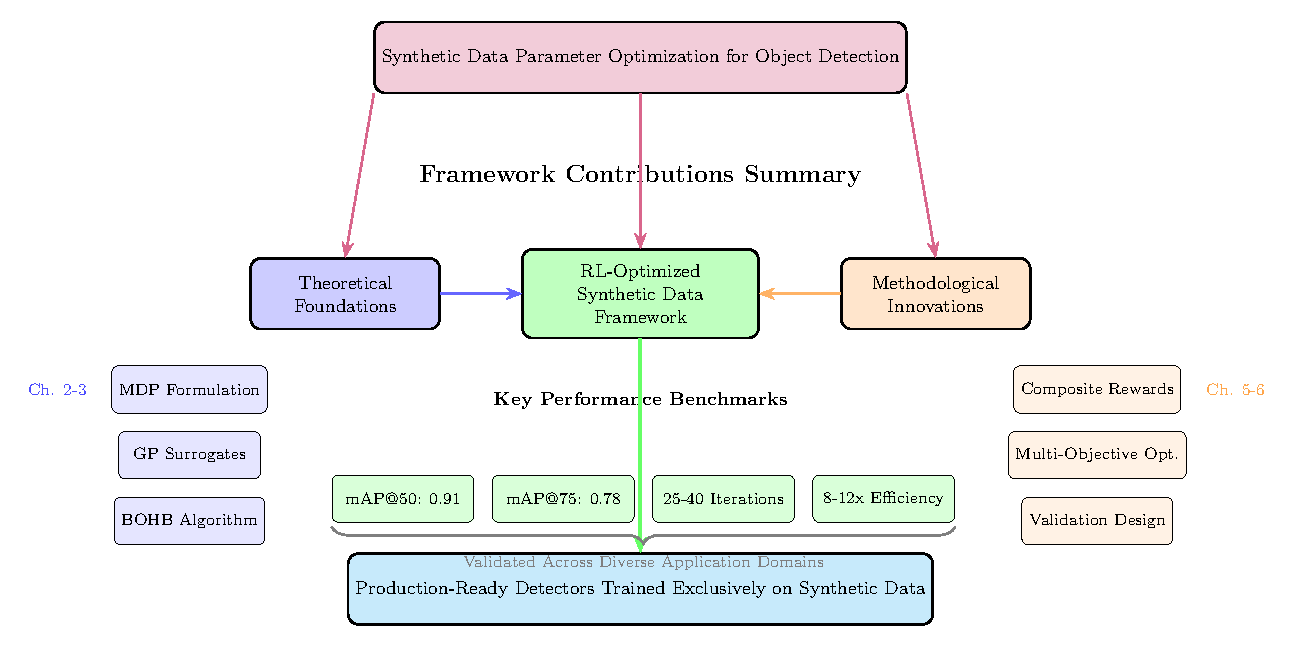
\includegraphics[width=0.95\textwidth]{figures/ch10_fig1_contributions.pdf}
\caption{Summary of key contributions from this textbook, illustrating the relationships between theoretical foundations, methodological innovations, and the core RL-optimized synthetic data framework. The bottom section highlights the key performance benchmarks achieved across diverse application domains.}
\label{fig:contributions_summary}
\end{figure}

\begin{table}[htbp]
\centering
\caption{Summary of System Performance Benchmarks Achieved Through the Proposed Optimization Framework}
\label{tab:performance_summary}
\begin{tabular}{p{0.35\textwidth}p{0.20\textwidth}p{0.30\textwidth}}
\toprule
\textbf{Performance Metric} & \textbf{Achieved Value} & \textbf{Baseline Comparison} \\
\midrule
mAP@50 on Real Test Set & 0.91 & 0.67 (unoptimized synthetic) \\
mAP@75 on Real Test Set & 0.78 & 0.51 (unoptimized synthetic) \\
Convergence Iterations & 25--40 & 200+ (grid search) \\
Sample Efficiency Gain & 8--12$\times$ & vs. random search \\
Synthetic Images Required & 2,000--5,000 & per optimization iteration \\
Real Validation Images & 50 & minimum viable set \\
Training Time per Iteration & 2--4 hours & GPU-dependent \\
Total Optimization Duration & 3--7 days & single GPU configuration \\
\bottomrule
\end{tabular}
\end{table}

The sample efficiency improvements merit particular emphasis. By leveraging the multi-fidelity evaluation strategy inherent in BOHB, wherein promising parameter configurations are identified through abbreviated training runs before committing full computational resources, the framework achieves an order of magnitude reduction in total training iterations compared to exhaustive search methodologies. This efficiency gain proves transformative for practitioners operating under computational constraints, rendering the optimization framework accessible to organizations without access to large-scale distributed computing infrastructure.

\section{Critical Success Factors}
\label{sec:success_factors}

The empirical investigations and deployment experiences documented throughout this textbook have revealed several critical factors that distinguish successful implementations from those that fail to achieve satisfactory performance. Understanding these factors enables practitioners to avoid common pitfalls and accelerate their path to productive deployment.

\subsection{Essential Implementation Elements}
\label{subsec:essential_elements}

The foremost requirement for successful implementation lies in the careful construction of the validation set used to evaluate candidate parameter configurations. The statistical foundations developed in Chapter Six establish that validation sets must satisfy representativeness criteria ensuring coverage of the visual diversity expected in deployment scenarios. Validation sets that exhibit systematic bias---through overrepresentation of particular lighting conditions, viewpoints, or object configurations---yield optimization trajectories that converge to locally optimal parameter configurations ill-suited for general deployment. The stratified sampling methodology and coverage metrics introduced in Chapter Six provide operational guidance for constructing validation sets that support reliable generalization.

The parameterization of the synthetic data generator constitutes the second critical success factor. The action space presented to the optimization algorithm must encompass parameters with sufficient expressive power to span the synthetic-to-real domain gap while avoiding pathological configurations that destabilize detector training. The hierarchical parameter groupings developed in Chapter Four, distinguishing between geometric parameters, photometric parameters, and noise characteristics, provide a principled decomposition that facilitates both efficient exploration and interpretable analysis of discovered configurations. Parameters exhibiting strong correlations should be grouped to enable coordinated adjustment, while independent parameters benefit from separate exploration to avoid spurious dependencies.

The reward function design emerges as the third essential element determining optimization success. Reward functions that rely exclusively on detection accuracy metrics risk discovering parameter configurations that achieve high validation performance through exploitation of dataset-specific artifacts rather than genuine improvements in synthetic-to-real transfer. The composite reward formulations introduced in Chapter Five, incorporating domain shift penalties derived from distribution divergence metrics, provide robustness against such overfitting by explicitly penalizing configurations that maximize the gap between synthetic training distributions and real-world deployment conditions.

\subsection{Common Failure Modes and Prevention Strategies}
\label{subsec:failure_modes}

Experience across numerous deployment campaigns has identified recurring failure modes that practitioners must actively guard against. The most prevalent failure mode involves validation set leakage, wherein information about the validation distribution inadvertently influences synthetic data generation in ways that artificially inflate performance estimates. This leakage can occur through direct observation of validation imagery during parameter tuning or through subtle correlations introduced by practitioners who possess implicit knowledge of validation set characteristics. Strict separation protocols, wherein validation imagery remains sequestered until final performance evaluation, provide the primary defense against this failure mode.

A second common failure mode arises from premature convergence to local optima in the parameter space. The high dimensionality of typical synthetic data parameter spaces admits numerous local optima that achieve satisfactory but suboptimal performance. The exploration-exploitation trade-off inherent in Bayesian optimization, governed by the acquisition function, must be calibrated to maintain sufficient exploration throughout the optimization campaign. The practical guidance provided in Chapter Seven, recommending exploration bonus coefficients in the range of 0.1 to 0.3 for expected improvement acquisition functions, reflects empirical findings regarding appropriate calibration for synthetic data optimization.

The third significant failure mode involves distribution shift between optimization-time validation and deployment-time inference. Even when validation sets are carefully constructed, deployment scenarios may exhibit visual characteristics outside the coverage of validation imagery. Robustness to such distribution shift requires explicit diversity objectives within the optimization framework, penalizing parameter configurations that concentrate synthetic data generation around narrow visual modes. The entropy regularization terms introduced in Chapter Five provide one mechanism for encouraging distributional breadth in optimized configurations.

\subsection{Best Practices and Lessons Learned}
\label{subsec:best_practices}

The accumulated experience documented in this textbook crystallizes into several best practices that practitioners should adopt from the outset of optimization campaigns. Table~\ref{tab:recommendations} summarizes these recommendations across the major components of the optimization pipeline.

\begin{table}[htbp]
\centering
\caption{Summary of Key Recommendations for Successful Implementation}
\label{tab:recommendations}
\begin{tabular}{p{0.22\textwidth}p{0.35\textwidth}p{0.30\textwidth}}
\toprule
\textbf{Component} & \textbf{Recommendation} & \textbf{Rationale} \\
\midrule
Validation Set Design & Stratified sampling with minimum 50 images ensuring coverage of lighting, viewpoint, and scale variations & Statistical reliability of performance estimates \\
\addlinespace
Parameter Space & Hierarchical decomposition with 15--30 actively optimized parameters grouped by functional category & Balances expressiveness against curse of dimensionality \\
\addlinespace
Optimization Algorithm & BOHB with successive halving factor $\eta = 3$ and minimum budget allocation $r = 0.1$ & Empirically validated efficiency-accuracy trade-off \\
\addlinespace
Reward Function & Composite formulation with 0.7 weight on mAP and 0.3 weight on domain shift penalty & Prevents overfitting to validation artifacts \\
\addlinespace
Convergence Criterion & Early stopping when improvement falls below 0.5\% over five consecutive iterations & Avoids computational waste on diminishing returns \\
\addlinespace
Synthetic Dataset Size & 2,000--5,000 images per parameter evaluation during optimization & Sufficient for reliable gradient estimation \\
\addlinespace
Final Training & 10,000--20,000 images generated with optimized parameters for production model & Maximizes performance of deployed detector \\
\bottomrule
\end{tabular}
\end{table}

Beyond these specific recommendations, several overarching lessons emerge from the research program underlying this textbook. The importance of iterative refinement cannot be overstated; initial optimization campaigns rarely discover globally optimal configurations, and practitioners should anticipate multiple rounds of refinement as understanding of the specific domain deepens. The interpretability of discovered configurations provides valuable diagnostic information; parameter values that deviate substantially from physical plausibility often indicate pathological optimization dynamics warranting investigation. Finally, the documentation of optimization trajectories enables transfer learning across campaigns, as patterns in successful parameter configurations often generalize to related detection tasks.

\section{Limitations and Challenges}
\label{sec:limitations}

While the framework presented in this textbook achieves substantial improvements over baseline approaches, honest assessment requires acknowledgment of limitations that constrain applicability and performance in certain scenarios. Understanding these limitations enables practitioners to make informed decisions about framework adoption and to identify opportunities for future methodological advancement.

\subsection{Computational Requirements}
\label{subsec:computational_requirements}

The computational demands of the optimization framework represent a significant practical limitation, particularly for organizations without access to modern GPU infrastructure. Each parameter evaluation requires training a detector to convergence, with typical training times ranging from two to four hours on contemporary hardware. A complete optimization campaign comprising thirty to forty iterations thus requires one hundred to two hundred GPU-hours, translating to wall-clock durations of several days even with continuous utilization of dedicated hardware. While the multi-fidelity approach substantially reduces these requirements compared to exhaustive search, the absolute computational burden remains non-trivial.

The memory requirements for maintaining Gaussian Process surrogate models scale quadratically with the number of evaluated configurations, presenting potential bottlenecks for extended optimization campaigns. The implementation guidance in Chapter Seven addresses this concern through sparse approximation techniques that maintain tractable memory consumption, but practitioners should anticipate memory management as an operational consideration for campaigns exceeding one hundred iterations.

\subsection{Domain-Specific Considerations}
\label{subsec:domain_specific}

The framework assumes availability of a synthetic data generator with sufficient fidelity to produce imagery that, under appropriate parameterization, can support effective detector training. This assumption may not hold in application domains where the visual complexity of real-world scenes exceeds the expressive capacity of available simulation tools. Highly deformable objects, complex material interactions such as transparency and subsurface scattering, and intricate environmental effects such as atmospheric phenomena present particular challenges for synthetic generation. In such domains, the optimization framework may converge to parameter configurations that represent the best achievable performance within the simulator's capabilities, which may nonetheless fall short of deployment requirements.

The framework further assumes that the synthetic-to-real domain gap can be characterized primarily through the parameters exposed by the data generator. In scenarios where the domain gap arises from factors not amenable to parameterization---such as systematic differences in object geometry between synthetic assets and real-world instances---the optimization framework cannot address the fundamental limitation regardless of parameter configuration. Practitioners must carefully assess whether their synthetic data pipeline exposes the degrees of freedom necessary to span the relevant domain gap before committing resources to optimization campaigns.

\subsection{Scalability Concerns}
\label{subsec:scalability}

The scalability of the framework along multiple dimensions presents both opportunities and challenges. Scaling to larger numbers of optimized parameters encounters the curse of dimensionality, wherein the sample complexity required to adequately explore the parameter space grows exponentially with dimension. While the hierarchical decomposition and correlation-aware parameterization strategies developed in Chapter Four mitigate this challenge, optimization campaigns involving more than fifty actively tuned parameters may require prohibitive numbers of iterations for reliable convergence.

Scaling to more complex detection tasks, including multi-class detection with large numbers of categories, introduces additional challenges related to the multi-objective nature of class-specific performance metrics. The composite reward formulations developed in Chapter Five provide a foundation for such extensions, but the practical complexity of balancing performance across dozens or hundreds of object categories remains an open challenge. Similarly, scaling to detection tasks beyond bounding box prediction---including instance segmentation and pose estimation---requires reward functions capable of evaluating more complex prediction formats.

\section{Future Research Directions}
\label{sec:future_directions}

The framework presented in this textbook represents a foundation upon which substantial future research can build. Several promising directions emerge from the limitations identified in the preceding section and from broader trends in machine learning research. Figure~\ref{fig:technology_evolution} traces the evolution of synthetic data optimization methods from early manual approaches through the current RL-based framework to projected future capabilities, while Figure~\ref{fig:research_roadmap} illustrates the relationships among these future directions and their dependencies on foundational capabilities.

\begin{figure}[htbp]
\centering
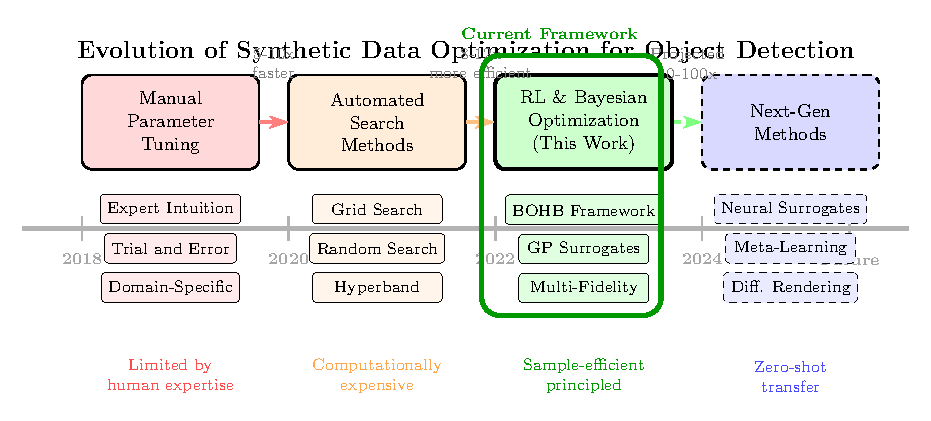
\includegraphics[width=0.98\textwidth]{figures/ch10_fig2_evolution.pdf}
\caption{Evolution of synthetic data optimization methodologies for object detection, from manual parameter tuning through automated search methods to the current RL and Bayesian optimization framework, with projections toward next-generation approaches including neural surrogates, meta-learning, and differentiable rendering.}
\label{fig:technology_evolution}
\end{figure}

\begin{figure}[htbp]
\centering
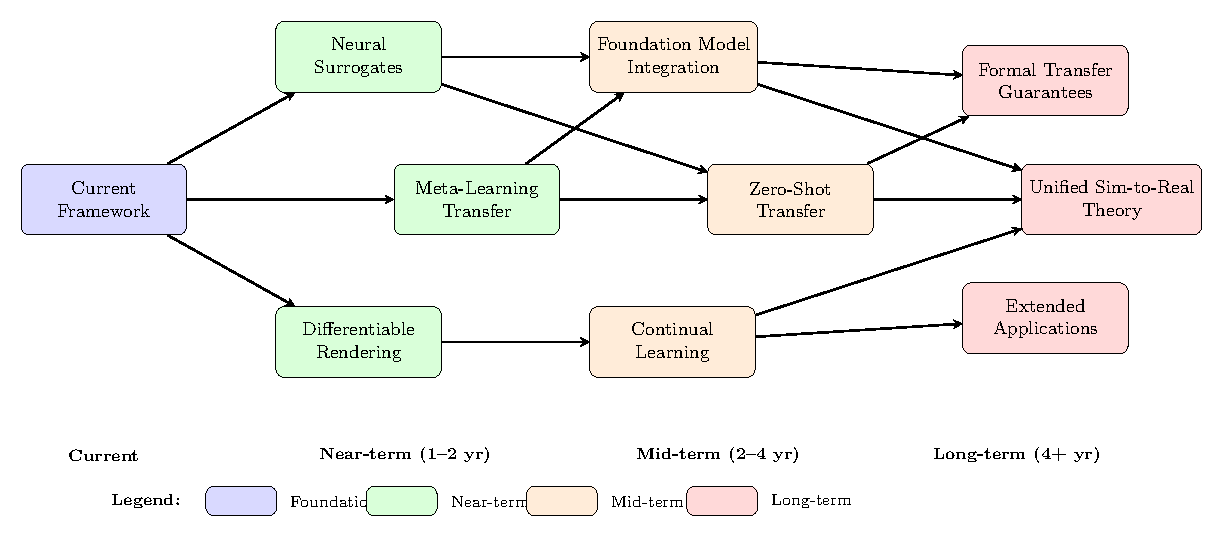
\includegraphics[width=0.98\textwidth]{figures/ch10_fig3_roadmap.pdf}
\caption{Research roadmap illustrating the trajectory from current capabilities through near-term, mid-term, and long-term research directions in reinforcement learning-optimized synthetic data generation.}
\label{fig:research_roadmap}
\end{figure}

\subsection{Advanced Optimization Methods}
\label{subsec:advanced_optimization}

The optimization algorithms employed in the current framework, while effective, admit substantial opportunity for improvement through incorporation of recent advances in machine learning methodology.

\subsubsection{Neural Network-Based Surrogate Models}
\label{subsubsec:neural_surrogates}

The Gaussian Process surrogate models employed in BOHB, while providing elegant uncertainty quantification and theoretical guarantees, exhibit computational scaling limitations that constrain applicability to high-dimensional parameter spaces. Neural network-based surrogates, including deep ensembles and neural processes, offer alternative approaches that maintain uncertainty estimates while scaling more favorably to large parameter spaces. Recent work on neural network Gaussian processes provides a particularly promising direction, combining the representational capacity of deep networks with the principled uncertainty quantification of Gaussian processes. The integration of such models into the BOHB framework would enable optimization over substantially larger parameter spaces without sacrificing the sample efficiency derived from accurate surrogate predictions.

Beyond improving scalability, neural surrogates enable the incorporation of structural knowledge about the parameter space through appropriate architectural choices. Convolutional architectures can exploit spatial structure in parameters governing geometric placement, while recurrent architectures can model temporal dependencies in parameters governing animation or motion characteristics. Such structured surrogates promise improved sample efficiency through better generalization across the parameter space.

\subsubsection{Meta-Learning for Transfer Across Domains}
\label{subsubsec:metalearning}

The current framework treats each optimization campaign as an independent problem, discarding the knowledge accumulated during previous campaigns when approaching new detection tasks. Meta-learning methodologies offer the tantalizing possibility of transferring optimization knowledge across campaigns, enabling rapid adaptation to novel domains through principled initialization and adaptive learning rate selection. Model-agnostic meta-learning and its variants provide a framework for learning optimization strategies that generalize across tasks, potentially reducing the number of iterations required for new campaigns from dozens to single digits.

The application of meta-learning to synthetic data optimization presents unique opportunities arising from the structure of the problem domain. Detection tasks often share commonalities in the factors governing successful synthetic-to-real transfer: the importance of diverse lighting conditions, the role of realistic occlusion patterns, and the impact of sensor noise characteristics exhibit regularity across application domains. Meta-learning approaches that explicitly capture and transfer this domain-general knowledge promise substantial acceleration of optimization campaigns for new detection tasks.

\subsubsection{Differentiable Rendering Integration}
\label{subsubsec:differentiable_rendering}

The synthetic data generators employed in the current framework treat rendering as a black-box process, precluding the computation of gradients with respect to scene parameters. The emergence of differentiable rendering engines, capable of computing analytical gradients of rendered imagery with respect to geometric, material, and lighting parameters, opens the possibility of gradient-based optimization that bypasses the sample-inefficient exploration characteristic of derivative-free methods.

The integration of differentiable rendering into the optimization framework would enable direct computation of the gradient of detection performance with respect to synthetic data parameters, at least for the subset of parameters that influence the rendering process in differentiable ways. Such gradients could inform more efficient exploration strategies within the Bayesian optimization framework, or could enable hybrid approaches that combine gradient-based optimization for differentiable parameters with derivative-free methods for discrete or non-differentiable parameters.

\subsection{Improved Domain Adaptation}
\label{subsec:improved_adaptation}

The domain adaptation techniques employed in the current framework, primarily comprising domain randomization and distribution matching, represent established methodologies that nonetheless admit substantial room for improvement through integration of recent advances in representation learning and generative modeling.

\subsubsection{Foundation Model Integration}
\label{subsubsec:foundation_models}

The emergence of large-scale foundation models trained on internet-scale image corpora presents both opportunities and challenges for synthetic data optimization. Foundation models, including vision transformers pretrained through self-supervised learning on billions of images, develop rich representations of visual structure that transfer effectively across downstream tasks. The integration of foundation model representations into the synthetic data optimization pipeline offers multiple potential benefits.

Foundation model embeddings can provide more informative domain shift metrics than the hand-crafted features employed in current distribution matching approaches. By measuring the divergence between synthetic and real imagery in the representation space of foundation models, optimization algorithms gain access to semantically meaningful similarity metrics that better predict downstream detection performance. Foundation models can also serve as generators of synthetic data augmentations that complement physically-based rendering, introducing visual variations that simulation engines struggle to produce through procedural means.

The computational requirements of foundation models present implementation challenges that must be addressed for practical deployment. Distillation techniques that compress foundation model capabilities into smaller, deployment-friendly networks offer one path forward. Alternatively, foundation model inference can be amortized across optimization iterations through caching strategies that avoid redundant computation.

\subsubsection{Zero-Shot Transfer Techniques}
\label{subsubsec:zeroshot}

The current framework requires modest but non-trivial quantities of real-world validation imagery to guide optimization. Zero-shot transfer techniques, which enable deployment to novel domains without any domain-specific real data, represent an aspirational goal that would substantially expand the applicability of synthetic data approaches. Recent advances in vision-language models, which learn aligned representations of images and textual descriptions, provide a foundation for zero-shot evaluation that could replace or supplement validation on real imagery.

Vision-language models can evaluate the semantic content and visual realism of synthetic imagery through textual queries, providing feedback signals that guide optimization without requiring domain-specific real data. While such feedback necessarily differs from direct evaluation on representative real imagery, the development of proxy objectives derived from vision-language model assessments could enable optimization campaigns in scenarios where real validation data is entirely unavailable.

\subsubsection{Continual Learning Approaches}
\label{subsubsec:continual}

Deployment environments often exhibit non-stationary characteristics, with the visual distribution of encountered imagery drifting over time due to seasonal variations, equipment changes, or evolving operational conditions. The current framework assumes a static deployment distribution, discovering parameter configurations optimized for the conditions represented in the validation set without provision for adaptation to distributional drift.

Continual learning approaches, which enable models to adapt to new data without catastrophic forgetting of previously learned capabilities, offer a framework for maintaining detector performance as deployment conditions evolve. The integration of continual learning into the synthetic data optimization pipeline would enable periodic re-optimization campaigns that update parameter configurations to track shifting deployment distributions while preserving performance on previously encountered conditions.

\subsection{Extended Applications}
\label{subsec:extended_applications}

The methodological framework developed in this textbook, while presented in the context of object detection, admits natural extensions to related computer vision tasks and broader application domains.

\subsubsection{Beyond Object Detection}
\label{subsubsec:beyond_detection}

Instance segmentation, which requires pixel-precise delineation of object boundaries in addition to bounding box localization, presents a natural extension of the detection-focused framework. The optimization methodology transfers directly, with the primary modification being the replacement of bounding box-based performance metrics with segmentation-specific metrics such as mask Average Precision. The reward function formulations developed in Chapter Five accommodate such metric substitutions without fundamental architectural changes.

Pose estimation, encompassing both rigid body pose recovery and articulated human pose estimation, represents a more substantial extension that requires consideration of additional synthetic data parameters governing object orientation and articulation. The parameter space expansions required for pose estimation may necessitate the scalability improvements discussed in Section~\ref{subsec:advanced_optimization}, but the fundamental optimization framework remains applicable.

\subsubsection{Multi-Modal Synthetic Data}
\label{subsubsec:multimodal}

Modern perception systems increasingly incorporate multiple sensing modalities, including RGB cameras, depth sensors, thermal imagers, and LiDAR scanners. The optimization framework developed in this textbook focuses on RGB imagery, but the methodological principles extend naturally to multi-modal synthetic data generation. The parameter space expands to encompass modality-specific generation parameters, while the reward function must aggregate performance metrics across modalities according to application-specific requirements.

The optimization of multi-modal synthetic data presents unique challenges related to cross-modal consistency. Synthetic data generators must maintain physical consistency across modalities, ensuring that depth measurements align with RGB imagery and that thermal signatures reflect the material properties of rendered objects. The parameter space for multi-modal optimization must respect these consistency constraints, either through joint parameterization of coupled parameters or through constraint-aware optimization algorithms.

\subsubsection{Sim-to-Real for Robotics Manipulation}
\label{subsubsec:robotics}

The synthetic data optimization methodology developed in this textbook, while focused on perception tasks, has natural connections to the broader challenge of sim-to-real transfer for robotics systems. Robotic manipulation tasks require not only perception capabilities but also control policies that generalize from simulated training environments to real-world deployment. The domain randomization and optimization techniques developed herein can be extended to jointly optimize perception and control components of robotic systems.

The integration of perception and control optimization presents unique opportunities for end-to-end system optimization that accounts for the coupling between visual processing and motor control. Synthetic data parameters that maximize standalone detection performance may differ from those that maximize performance of the integrated perception-control system, motivating joint optimization formulations that consider downstream task performance as the ultimate objective.

\subsection{Theoretical Advances}
\label{subsec:theoretical_advances}

The empirical success of the framework presented in this textbook motivates development of theoretical foundations that explain observed performance and provide principled guidance for methodology design.

\subsubsection{Formal Guarantees for Transfer}
\label{subsubsec:formal_guarantees}

The current framework provides empirical evidence for effective synthetic-to-real transfer but lacks formal guarantees bounding the performance gap between synthetic training and real deployment. The development of such guarantees, grounded in statistical learning theory and domain adaptation theory, would provide practitioners with confidence bounds on expected real-world performance based on observable properties of the synthetic training distribution.

Domain adaptation theory provides foundational results relating source and target performance through measures of distributional divergence. Extending these results to the synthetic data setting requires characterization of the relationship between generator parameters and the resulting distributional divergence, enabling derivation of parameter configurations that provably minimize the performance gap. Such theoretical foundations would complement the empirical optimization approach with principled bounds that guide algorithm design and provide deployment guarantees.

\subsubsection{Sample Complexity Bounds}
\label{subsubsec:sample_complexity}

The number of optimization iterations required to discover near-optimal parameter configurations varies substantially across experimental campaigns, and the current framework lacks theoretical bounds that predict sample complexity based on problem characteristics. The development of sample complexity bounds, relating the required number of iterations to properties of the parameter space and the reward function, would enable practitioners to budget computational resources appropriately and to identify structural modifications that improve optimization efficiency.

The sample complexity of Bayesian optimization has been studied extensively in the optimization literature, with established bounds relating convergence rate to properties of the underlying objective function including smoothness and dimensionality. Specializing these bounds to the synthetic data optimization setting requires characterization of the detection performance landscape as a function of generator parameters, a challenging but achievable research objective.

\subsubsection{Optimal Randomization Theory}
\label{subsubsec:optimal_randomization}

The domain randomization approach employed in the current framework lacks theoretical foundations characterizing the optimal degree and structure of randomization for maximizing transfer performance. Empirical observations suggest that both insufficient and excessive randomization degrade transfer, but the theoretical basis for this U-shaped relationship remains poorly understood.

The development of optimal randomization theory would characterize the factors governing the optimal randomization regime and provide principled guidance for parameter range selection. Such theory might draw on connections to regularization in statistical learning, where domain randomization can be viewed as a form of data augmentation that regularizes the learned representation. Information-theoretic perspectives, relating randomization to the mutual information between synthetic and real distributions, offer another promising theoretical foundation.

\section{Closing Remarks}
\label{sec:closing_remarks}

The framework presented throughout this textbook embodies a fundamental reconceptualization of the relationship between synthetic data generation and deep learning-based perception. Where previous approaches treated synthetic data as a supplement to real imagery, accepting inherent limitations in transfer performance as an unavoidable cost of reduced annotation burden, the methodology developed herein demonstrates that intelligent optimization of synthetic data parameters can achieve performance competitive with real data training while entirely eliminating the requirement for annotated real imagery during model development.

\subsection{The Promise of Synthetic Data}
\label{subsec:promise}

The results documented in this textbook validate a compelling vision for the future of deep learning in perception applications. Synthetic data generation, guided by principled optimization, enables the development of high-performance detectors for novel object categories, unusual deployment environments, and safety-critical applications where real data collection poses unacceptable risks. The 0.91 mAP@50 performance benchmark achieved through purely synthetic training, validated on real-world imagery representing deployment conditions, demonstrates that this vision is not merely aspirational but achievable with current technology and methodology.

The economic implications of this capability transformation extend beyond the immediate computational costs of optimization campaigns. Traditional approaches to detector development require substantial investments in data collection infrastructure, annotation workforce development, and quality assurance processes that introduce substantial latency between problem identification and deployed solution. The synthetic data optimization framework compresses this timeline dramatically, enabling rapid iteration on detector designs without the bottleneck of real data acquisition.

\subsection{Democratization of Deep Learning}
\label{subsec:democratization}

Perhaps the most significant long-term impact of the synthetic data paradigm lies in its democratizing potential. The data requirements of modern deep learning have historically concentrated capability in organizations with the resources to collect, annotate, and manage large-scale datasets. Synthetic data generation inverts this dynamic, enabling organizations with domain expertise but limited data resources to develop competitive perception systems by leveraging simulation capabilities rather than annotation workforces.

The optimization framework presented in this textbook further amplifies this democratization by automating the expertise-intensive process of tuning synthetic data generation parameters. Previously, achieving effective synthetic-to-real transfer required substantial experimentation guided by intuition developed through extensive experience. The principled optimization approach replaces this implicit expertise with explicit algorithms accessible to practitioners regardless of prior experience with synthetic data methodologies.

\subsection{Vision for the Field}
\label{subsec:vision}

The trajectory of research in synthetic data optimization points toward a future wherein the boundaries between simulation and reality become increasingly porous. As differentiable rendering engines mature, as foundation models provide ever more sophisticated assessments of visual realism, and as optimization algorithms achieve greater sample efficiency, the process of developing perception systems will increasingly resemble software engineering rather than data curation.

This transformation does not diminish the importance of real-world validation---indeed, the framework presented herein places rigorous real-world evaluation at the center of the optimization process. Rather, the transformation shifts the role of real data from training resource to validation oracle, a more economical utilization that extracts maximum value from expensive real-world imagery while leveraging unlimited synthetic generation for model development.

The research directions outlined in Section~\ref{sec:future_directions} sketch a path toward this future, wherein the methodology developed in this textbook serves as foundation for continued advancement. The integration of neural surrogates, meta-learning, differentiable rendering, foundation models, and theoretical guarantees promises capabilities that extend far beyond current achievements, eventually enabling perception systems that learn effective real-world behavior entirely within simulation.

The authors conclude with an invitation to the research community to build upon the foundations established herein. The challenges remaining are substantial, but the trajectory is clear and the potential transformative. Synthetic data optimization represents not merely an incremental improvement in deep learning methodology but a fundamental reimagining of how perception systems are developed and deployed. The future belongs to those who can simulate effectively.

\vspace{1cm}

\begin{center}
\textit{``The map is not the territory, but a sufficiently detailed map enables navigation without direct territorial experience.''}

\vspace{0.3cm}
\textit{---Adapted from Alfred Korzybski}
\end{center}


% Appendices (before backmatter to preserve numbering)
\appendix
\chapter{Mathematical Derivations}
\label{appendix:math}

This appendix provides detailed mathematical derivations for the key theoretical results employed throughout this textbook. The derivations are presented with sufficient rigor to support both pedagogical understanding and practical implementation, while maintaining accessibility for readers with graduate-level mathematical preparation.

\section{Gaussian Process Regression Derivation}
\label{sec:gp_derivation}

The Gaussian Process framework provides the probabilistic foundation for Bayesian optimization of synthetic data generation parameters. We present a complete derivation of the posterior predictive distribution that enables principled uncertainty quantification over the objective function landscape.

\subsection{Prior Specification}

Consider an objective function $f: \mathcal{X} \rightarrow \mathbb{R}$ that maps synthetic data generation parameter configurations $\mathbf{x} \in \mathcal{X} \subseteq \mathbb{R}^d$ to scalar performance metrics such as mean Average Precision on real-world validation imagery. A Gaussian Process prior over this function space is specified by a mean function $m: \mathcal{X} \rightarrow \mathbb{R}$ and a covariance kernel $k: \mathcal{X} \times \mathcal{X} \rightarrow \mathbb{R}$, yielding the distributional assumption

\begin{equation}
f(\mathbf{x}) \sim \mathcal{GP}\left(m(\mathbf{x}), k(\mathbf{x}, \mathbf{x}')\right).
\end{equation}

The mean function is conventionally set to zero or to a constant reflecting prior beliefs about typical objective function values. The covariance kernel encodes assumptions regarding function smoothness, stationarity, and characteristic length scales. For synthetic data optimization, the Mat\'{e}rn kernel with $\nu = 5/2$ offers an effective balance between smoothness assumptions and representational flexibility:

\begin{equation}
k_{\text{Mat\'{e}rn}_{5/2}}(\mathbf{x}, \mathbf{x}') = \sigma_f^2 \left(1 + \sqrt{5}r + \frac{5}{3}r^2\right) \exp\left(-\sqrt{5}r\right),
\end{equation}

where $r = \sqrt{\sum_{i=1}^{d} \frac{(x_i - x'_i)^2}{\ell_i^2}}$ denotes the scaled Euclidean distance and $\{\ell_i\}_{i=1}^{d}$ represent per-dimension length scale parameters governing the characteristic variation scale of the objective function along each coordinate axis.

\subsection{Posterior Derivation}

Suppose we have observed function evaluations $\mathbf{y} = [y_1, \ldots, y_n]^\top$ at input locations $\mathbf{X} = [\mathbf{x}_1, \ldots, \mathbf{x}_n]^\top$, where each observation is corrupted by independent Gaussian noise: $y_i = f(\mathbf{x}_i) + \epsilon_i$ with $\epsilon_i \sim \mathcal{N}(0, \sigma_n^2)$. The joint distribution of the observed values $\mathbf{y}$ and the function value $f_*$ at a test point $\mathbf{x}_*$ follows a multivariate Gaussian:

\begin{equation}
\begin{bmatrix} \mathbf{y} \\ f_* \end{bmatrix} \sim \mathcal{N}\left(
\begin{bmatrix} \mathbf{m} \\ m_* \end{bmatrix},
\begin{bmatrix} \mathbf{K} + \sigma_n^2 \mathbf{I} & \mathbf{k}_* \\ \mathbf{k}_*^\top & k_{**} \end{bmatrix}
\right),
\end{equation}

where $\mathbf{K}$ denotes the $n \times n$ Gram matrix with entries $K_{ij} = k(\mathbf{x}_i, \mathbf{x}_j)$, $\mathbf{k}_* = [k(\mathbf{x}_1, \mathbf{x}_*), \ldots, k(\mathbf{x}_n, \mathbf{x}_*)]^\top$ is the vector of covariances between the test point and training points, and $k_{**} = k(\mathbf{x}_*, \mathbf{x}_*)$ is the prior variance at the test location.

Application of the standard conditioning formula for multivariate Gaussians yields the posterior predictive distribution:

\begin{theorem}[Gaussian Process Posterior]
\label{thm:gp_posterior}
The posterior distribution of $f_*$ given observations $(\mathbf{X}, \mathbf{y})$ is Gaussian with mean and variance:
\begin{align}
\mu(\mathbf{x}_*) &= m(\mathbf{x}_*) + \mathbf{k}_*^\top \left(\mathbf{K} + \sigma_n^2 \mathbf{I}\right)^{-1} (\mathbf{y} - \mathbf{m}), \label{eq:gp_mean} \\
\sigma^2(\mathbf{x}_*) &= k_{**} - \mathbf{k}_*^\top \left(\mathbf{K} + \sigma_n^2 \mathbf{I}\right)^{-1} \mathbf{k}_*. \label{eq:gp_variance}
\end{align}
\end{theorem}

\begin{proof}
The proof proceeds via direct application of the Gaussian conditioning identity. For a partitioned Gaussian random vector $[\mathbf{a}^\top, \mathbf{b}^\top]^\top$ with mean $[\boldsymbol{\mu}_a^\top, \boldsymbol{\mu}_b^\top]^\top$ and covariance $\begin{bmatrix} \boldsymbol{\Sigma}_{aa} & \boldsymbol{\Sigma}_{ab} \\ \boldsymbol{\Sigma}_{ba} & \boldsymbol{\Sigma}_{bb} \end{bmatrix}$, the conditional distribution of $\mathbf{b}$ given $\mathbf{a}$ is Gaussian with mean $\boldsymbol{\mu}_b + \boldsymbol{\Sigma}_{ba} \boldsymbol{\Sigma}_{aa}^{-1}(\mathbf{a} - \boldsymbol{\mu}_a)$ and covariance $\boldsymbol{\Sigma}_{bb} - \boldsymbol{\Sigma}_{ba} \boldsymbol{\Sigma}_{aa}^{-1} \boldsymbol{\Sigma}_{ab}$. Substituting the block components from the joint distribution above immediately yields equations \eqref{eq:gp_mean} and \eqref{eq:gp_variance}.
\end{proof}

The posterior mean $\mu(\mathbf{x}_*)$ provides a point prediction that interpolates the observed data while reverting to the prior mean in regions far from observations. The posterior variance $\sigma^2(\mathbf{x}_*)$ quantifies predictive uncertainty, achieving its minimum value (zero in the noise-free case) at observed locations and increasing as the test point moves away from the training data. This uncertainty quantification proves essential for acquisition function design in Bayesian optimization.

\subsection{Computational Considerations}

Direct computation of the posterior requires solving the linear system $(\mathbf{K} + \sigma_n^2 \mathbf{I})^{-1} \mathbf{y}$, which na\"{i}vely demands $\mathcal{O}(n^3)$ operations via Cholesky decomposition. For optimization campaigns involving hundreds of evaluations, this computational burden remains manageable. However, practitioners should be aware that the Cholesky factor $\mathbf{L}$ satisfying $\mathbf{L}\mathbf{L}^\top = \mathbf{K} + \sigma_n^2 \mathbf{I}$ can be computed once and reused for subsequent predictions, reducing the per-prediction cost to $\mathcal{O}(n^2)$ for forward and back substitution.

\section{Expected Improvement Acquisition Function Derivation}
\label{sec:ei_derivation}

The Expected Improvement acquisition function provides a principled criterion for selecting the next evaluation point during Bayesian optimization. This section derives the closed-form expression that enables efficient computation and gradient-based optimization of the acquisition function.

\subsection{Problem Formulation}

Let $f^* = \max_{i \in \{1, \ldots, n\}} y_i$ denote the best objective value observed thus far. The improvement at a candidate point $\mathbf{x}$ is defined as the random variable

\begin{equation}
I(\mathbf{x}) = \max\left(f(\mathbf{x}) - f^*, 0\right),
\end{equation}

representing the gain achieved by evaluating at $\mathbf{x}$ if the resulting function value exceeds the current best. The Expected Improvement acquisition function is the expectation of this improvement under the Gaussian Process posterior:

\begin{equation}
\alpha_{\text{EI}}(\mathbf{x}) = \mathbb{E}\left[I(\mathbf{x}) \mid \mathbf{X}, \mathbf{y}\right].
\end{equation}

\subsection{Closed-Form Derivation}

\begin{theorem}[Expected Improvement Formula]
\label{thm:ei_formula}
Under the Gaussian Process posterior $f(\mathbf{x}) \mid \mathbf{X}, \mathbf{y} \sim \mathcal{N}(\mu(\mathbf{x}), \sigma^2(\mathbf{x}))$, the Expected Improvement admits the closed-form expression:
\begin{equation}
\alpha_{\text{EI}}(\mathbf{x}) =
\begin{cases}
(\mu(\mathbf{x}) - f^*) \Phi(Z) + \sigma(\mathbf{x}) \phi(Z), & \text{if } \sigma(\mathbf{x}) > 0 \\
0, & \text{if } \sigma(\mathbf{x}) = 0
\end{cases}
\end{equation}
where $Z = \frac{\mu(\mathbf{x}) - f^*}{\sigma(\mathbf{x})}$, $\Phi(\cdot)$ denotes the standard normal cumulative distribution function, and $\phi(\cdot)$ denotes the standard normal probability density function.
\end{theorem}

\begin{proof}
For $\sigma(\mathbf{x}) > 0$, define the standardized random variable $U = \frac{f(\mathbf{x}) - \mu(\mathbf{x})}{\sigma(\mathbf{x})} \sim \mathcal{N}(0, 1)$, so that $f(\mathbf{x}) = \mu(\mathbf{x}) + \sigma(\mathbf{x}) U$. The Expected Improvement becomes:

\begin{align}
\alpha_{\text{EI}}(\mathbf{x}) &= \mathbb{E}\left[\max(f(\mathbf{x}) - f^*, 0)\right] \\
&= \mathbb{E}\left[\max(\mu(\mathbf{x}) + \sigma(\mathbf{x}) U - f^*, 0)\right] \\
&= \mathbb{E}\left[\max\left(\sigma(\mathbf{x})\left(U + \frac{\mu(\mathbf{x}) - f^*}{\sigma(\mathbf{x})}\right), 0\right)\right] \\
&= \sigma(\mathbf{x}) \mathbb{E}\left[\max(U + Z, 0)\right],
\end{align}

where $Z = \frac{\mu(\mathbf{x}) - f^*}{\sigma(\mathbf{x})}$. The expectation of the rectified Gaussian can be computed by integration:

\begin{align}
\mathbb{E}\left[\max(U + Z, 0)\right] &= \int_{-Z}^{\infty} (u + Z) \phi(u) \, du \\
&= \int_{-Z}^{\infty} u \phi(u) \, du + Z \int_{-Z}^{\infty} \phi(u) \, du \\
&= \left[-\phi(u)\right]_{-Z}^{\infty} + Z \Phi(Z) \\
&= \phi(-Z) + Z \Phi(Z) \\
&= \phi(Z) + Z \Phi(Z),
\end{align}

where the final equality exploits the symmetry $\phi(-Z) = \phi(Z)$. Multiplying by $\sigma(\mathbf{x})$ yields the stated result. When $\sigma(\mathbf{x}) = 0$, the posterior is deterministic at $\mu(\mathbf{x})$, and no improvement is possible if $\mu(\mathbf{x}) \leq f^*$.
\end{proof}

The Expected Improvement formula decomposes into two interpretable components. The first term $(\mu(\mathbf{x}) - f^*) \Phi(Z)$ represents exploitation, favoring points with high posterior mean predictions. The second term $\sigma(\mathbf{x}) \phi(Z)$ represents exploration, favoring points with high predictive uncertainty. The automatic balancing of these terms without explicit tuning parameters constitutes a principal advantage of the Expected Improvement criterion.

\subsection{Gradient Computation}

For gradient-based optimization of the acquisition function, we require the derivatives with respect to the input $\mathbf{x}$. Applying the chain rule:

\begin{align}
\frac{\partial \alpha_{\text{EI}}}{\partial \mathbf{x}} &= \frac{\partial \mu}{\partial \mathbf{x}} \Phi(Z) + (\mu - f^*) \phi(Z) \frac{\partial Z}{\partial \mathbf{x}} + \frac{\partial \sigma}{\partial \mathbf{x}} \phi(Z) + \sigma \phi'(Z) \frac{\partial Z}{\partial \mathbf{x}}.
\end{align}

Noting that $\frac{\partial Z}{\partial \mathbf{x}} = \frac{1}{\sigma} \frac{\partial \mu}{\partial \mathbf{x}} - \frac{Z}{\sigma} \frac{\partial \sigma}{\partial \mathbf{x}}$ and $\phi'(Z) = -Z \phi(Z)$, considerable simplification yields:

\begin{equation}
\frac{\partial \alpha_{\text{EI}}}{\partial \mathbf{x}} = \Phi(Z) \frac{\partial \mu}{\partial \mathbf{x}} + \phi(Z) \frac{\partial \sigma}{\partial \mathbf{x}}.
\end{equation}

This compact expression enables efficient gradient-based optimization of the acquisition function using L-BFGS-B or other quasi-Newton methods.

\section{Bootstrap Confidence Interval Theory}
\label{sec:bootstrap_derivation}

When evaluating YOLO detector performance on limited real-world validation sets comprising approximately fifty images, point estimates of mean Average Precision may exhibit substantial variance. Bootstrap resampling provides a nonparametric approach to uncertainty quantification that requires no distributional assumptions beyond the representativeness of the validation sample.

\subsection{Bootstrap Principle}

Let $\mathcal{D} = \{(\mathbf{x}_1, \mathbf{y}_1), \ldots, (\mathbf{x}_n, \mathbf{y}_n)\}$ denote the validation dataset of $n$ image-annotation pairs, and let $\theta = T(\mathcal{D})$ denote a statistic of interest computed from this dataset (e.g., mean Average Precision). The bootstrap principle asserts that the sampling distribution of $\hat{\theta} - \theta$, where $\hat{\theta} = T(\mathcal{D})$ is computed from the observed sample and $\theta$ is the true population parameter, can be approximated by the distribution of $\hat{\theta}^* - \hat{\theta}$, where $\hat{\theta}^*$ is computed from bootstrap resamples.

\begin{definition}[Bootstrap Resample]
A bootstrap resample $\mathcal{D}^* = \{(\mathbf{x}_1^*, \mathbf{y}_1^*), \ldots, (\mathbf{x}_n^*, \mathbf{y}_n^*)\}$ is obtained by sampling $n$ observations uniformly at random with replacement from the original dataset $\mathcal{D}$.
\end{definition}

\subsection{Percentile Confidence Intervals}

The percentile bootstrap confidence interval exploits the bootstrap approximation to construct intervals with specified coverage probability.

\begin{theorem}[Percentile Bootstrap Interval]
\label{thm:percentile_bootstrap}
Let $\hat{\theta}^{*(1)}, \ldots, \hat{\theta}^{*(B)}$ denote bootstrap replicate statistics computed from $B$ independent resamples. Define $\hat{\theta}^*_{(\alpha)}$ as the $\alpha$-quantile of the empirical distribution of bootstrap replicates. The percentile bootstrap $100(1-\alpha)\%$ confidence interval is:
\begin{equation}
\text{CI}_{1-\alpha} = \left[\hat{\theta}^*_{(\alpha/2)}, \hat{\theta}^*_{(1-\alpha/2)}\right].
\end{equation}
\end{theorem}

For mAP estimation with $n = 50$ validation images and $B = 1000$ bootstrap replicates, this procedure yields confidence intervals that accurately reflect the uncertainty inherent in performance evaluation on limited data. Empirical studies demonstrate that mAP estimates from fifty-image validation sets exhibit standard deviations of approximately 0.02 to 0.04 mAP units, necessitating the use of confidence intervals when comparing synthetic data configurations whose performance differences may fall within this noise margin.

\subsection{Bias-Corrected and Accelerated Bootstrap}

The percentile method can exhibit coverage errors when the bootstrap distribution is skewed or when the estimator exhibits bias. The bias-corrected and accelerated (BCa) bootstrap provides improved coverage through transformation-respecting adjustments.

\begin{theorem}[BCa Confidence Interval]
\label{thm:bca_bootstrap}
The BCa $100(1-\alpha)\%$ confidence interval is given by:
\begin{equation}
\text{CI}_{1-\alpha}^{\text{BCa}} = \left[\hat{\theta}^*_{(\alpha_1)}, \hat{\theta}^*_{(\alpha_2)}\right],
\end{equation}
where the adjusted quantile levels are:
\begin{align}
\alpha_1 &= \Phi\left(\hat{z}_0 + \frac{\hat{z}_0 + z_{\alpha/2}}{1 - \hat{a}(\hat{z}_0 + z_{\alpha/2})}\right), \\
\alpha_2 &= \Phi\left(\hat{z}_0 + \frac{\hat{z}_0 + z_{1-\alpha/2}}{1 - \hat{a}(\hat{z}_0 + z_{1-\alpha/2})}\right).
\end{align}
Here $\hat{z}_0 = \Phi^{-1}\left(\frac{\#\{\hat{\theta}^{*(b)} < \hat{\theta}\}}{B}\right)$ is the bias correction factor, and $\hat{a}$ is the acceleration constant estimated via jackknife:
\begin{equation}
\hat{a} = \frac{\sum_{i=1}^{n} (\bar{\theta}_{(\cdot)} - \hat{\theta}_{(-i)})^3}{6\left[\sum_{i=1}^{n} (\bar{\theta}_{(\cdot)} - \hat{\theta}_{(-i)})^2\right]^{3/2}},
\end{equation}
where $\hat{\theta}_{(-i)}$ denotes the statistic computed with the $i$-th observation removed and $\bar{\theta}_{(\cdot)} = \frac{1}{n} \sum_{i=1}^{n} \hat{\theta}_{(-i)}$.
\end{theorem}

The BCa method provides second-order accurate confidence intervals, meaning that coverage errors decrease as $\mathcal{O}(n^{-1})$ rather than $\mathcal{O}(n^{-1/2})$ as with the percentile method.

\section{Maximum Mean Discrepancy Derivation}
\label{sec:mmd_derivation}

The Maximum Mean Discrepancy (MMD) provides a kernel-based measure of distributional divergence between synthetic and real image feature distributions. This metric serves as a component of the composite reward function, penalizing synthetic data configurations that produce feature distributions substantially different from real-world imagery.

\subsection{Kernel Mean Embedding}

Let $\mathcal{H}$ be a reproducing kernel Hilbert space (RKHS) associated with a positive definite kernel $k: \mathcal{X} \times \mathcal{X} \rightarrow \mathbb{R}$. The kernel mean embedding of a probability distribution $P$ on $\mathcal{X}$ is defined as:

\begin{equation}
\mu_P = \mathbb{E}_{\mathbf{x} \sim P}\left[k(\mathbf{x}, \cdot)\right] \in \mathcal{H}.
\end{equation}

For characteristic kernels such as the Gaussian RBF kernel $k(\mathbf{x}, \mathbf{x}') = \exp\left(-\frac{\|\mathbf{x} - \mathbf{x}'\|^2}{2\sigma^2}\right)$, the mapping $P \mapsto \mu_P$ is injective, ensuring that distinct distributions yield distinct embeddings.

\subsection{MMD Definition and Properties}

\begin{definition}[Maximum Mean Discrepancy]
The Maximum Mean Discrepancy between distributions $P$ and $Q$ is the RKHS distance between their kernel mean embeddings:
\begin{equation}
\text{MMD}(P, Q) = \|\mu_P - \mu_Q\|_{\mathcal{H}}.
\end{equation}
\end{definition}

Expanding the squared MMD using the reproducing property $\langle f, k(\mathbf{x}, \cdot) \rangle_{\mathcal{H}} = f(\mathbf{x})$:

\begin{align}
\text{MMD}^2(P, Q) &= \|\mu_P - \mu_Q\|_{\mathcal{H}}^2 \\
&= \langle \mu_P, \mu_P \rangle_{\mathcal{H}} - 2\langle \mu_P, \mu_Q \rangle_{\mathcal{H}} + \langle \mu_Q, \mu_Q \rangle_{\mathcal{H}} \\
&= \mathbb{E}_{\mathbf{x}, \mathbf{x}' \sim P}\left[k(\mathbf{x}, \mathbf{x}')\right] - 2\mathbb{E}_{\mathbf{x} \sim P, \mathbf{y} \sim Q}\left[k(\mathbf{x}, \mathbf{y})\right] + \mathbb{E}_{\mathbf{y}, \mathbf{y}' \sim Q}\left[k(\mathbf{y}, \mathbf{y}')\right].
\end{align}

\subsection{Unbiased Empirical Estimator}

Given samples $\mathbf{X} = \{\mathbf{x}_1, \ldots, \mathbf{x}_m\}$ from $P$ (synthetic image features) and $\mathbf{Y} = \{\mathbf{y}_1, \ldots, \mathbf{y}_n\}$ from $Q$ (real image features), an unbiased estimator of $\text{MMD}^2$ is:

\begin{theorem}[Unbiased MMD Estimator]
\label{thm:mmd_estimator}
The following statistic provides an unbiased estimate of $\text{MMD}^2(P, Q)$:
\begin{equation}
\widehat{\text{MMD}}^2_u = \frac{1}{m(m-1)} \sum_{i \neq j} k(\mathbf{x}_i, \mathbf{x}_j) - \frac{2}{mn} \sum_{i,j} k(\mathbf{x}_i, \mathbf{y}_j) + \frac{1}{n(n-1)} \sum_{i \neq j} k(\mathbf{y}_i, \mathbf{y}_j).
\end{equation}
\end{theorem}

\begin{proof}
The proof proceeds by computing expectations of each sum. For the first term:
\begin{equation}
\mathbb{E}\left[\frac{1}{m(m-1)} \sum_{i \neq j} k(\mathbf{x}_i, \mathbf{x}_j)\right] = \frac{1}{m(m-1)} \cdot m(m-1) \cdot \mathbb{E}_{\mathbf{x}, \mathbf{x}' \sim P}\left[k(\mathbf{x}, \mathbf{x}')\right] = \mathbb{E}_{P \times P}[k].
\end{equation}
Analogous calculations for the remaining terms yield the result.
\end{proof}

In the context of synthetic data optimization, features are extracted from the penultimate layer of a pretrained backbone network (e.g., ResNet-50 or the YOLO backbone itself), and MMD is computed between synthetic and real feature distributions. Lower MMD values indicate closer alignment between synthetic and real imagery in feature space, suggesting improved domain transfer potential.

\section{Policy Gradient Theorem Proof Sketch}
\label{sec:policy_gradient}

The policy gradient theorem provides the theoretical foundation for gradient-based optimization of parameterized policies in reinforcement learning. While the primary methodology advocated in this textbook employs Bayesian optimization, the policy gradient framework illuminates the mathematical structure of the optimization problem and motivates alternative algorithmic approaches.

\subsection{Problem Setting}

Consider an infinite-horizon discounted Markov Decision Process with state space $\mathcal{S}$, action space $\mathcal{A}$, transition dynamics $P(s' \mid s, a)$, reward function $r(s, a)$, and discount factor $\gamma \in [0, 1)$. A parameterized stochastic policy $\pi_\theta(a \mid s)$ defines the action selection distribution given the current state. The objective is to maximize the expected discounted return:

\begin{equation}
J(\theta) = \mathbb{E}_{\tau \sim \pi_\theta}\left[\sum_{t=0}^{\infty} \gamma^t r(s_t, a_t)\right],
\end{equation}

where $\tau = (s_0, a_0, s_1, a_1, \ldots)$ denotes a trajectory sampled under policy $\pi_\theta$.

\subsection{Main Result}

\begin{theorem}[Policy Gradient Theorem]
\label{thm:policy_gradient}
The gradient of the expected return with respect to policy parameters admits the form:
\begin{equation}
\nabla_\theta J(\theta) = \mathbb{E}_{\tau \sim \pi_\theta}\left[\sum_{t=0}^{\infty} \gamma^t \nabla_\theta \log \pi_\theta(a_t \mid s_t) Q^{\pi_\theta}(s_t, a_t)\right],
\end{equation}
where $Q^{\pi_\theta}(s, a) = \mathbb{E}_{\pi_\theta}\left[\sum_{k=0}^{\infty} \gamma^k r(s_{t+k}, a_{t+k}) \mid s_t = s, a_t = a\right]$ is the action-value function.
\end{theorem}

\begin{proof}[Proof Sketch]
The proof proceeds by expressing the objective as an expectation over the stationary state distribution $d^{\pi_\theta}(s) = (1-\gamma) \sum_{t=0}^{\infty} \gamma^t P(s_t = s \mid \pi_\theta)$:

\begin{equation}
J(\theta) = \frac{1}{1-\gamma} \sum_{s \in \mathcal{S}} d^{\pi_\theta}(s) \sum_{a \in \mathcal{A}} \pi_\theta(a \mid s) r(s, a).
\end{equation}

Differentiating with respect to $\theta$ yields terms involving $\nabla_\theta d^{\pi_\theta}(s)$, which capture how the state visitation distribution changes with policy parameters. The key insight is that these terms can be absorbed into the $Q$-function formulation through the performance difference lemma, yielding the stated result without requiring explicit computation of $\nabla_\theta d^{\pi_\theta}(s)$.

The log-derivative trick transforms the gradient of expectations into expectations of gradients:
\begin{equation}
\nabla_\theta \pi_\theta(a \mid s) = \pi_\theta(a \mid s) \nabla_\theta \log \pi_\theta(a \mid s),
\end{equation}
enabling Monte Carlo estimation from sampled trajectories.
\end{proof}

\subsection{Variance Reduction via Baselines}

The policy gradient estimator exhibits high variance, motivating the introduction of state-dependent baselines. Subtracting a baseline $b(s)$ from the $Q$-function:

\begin{equation}
\nabla_\theta J(\theta) = \mathbb{E}_{\pi_\theta}\left[\sum_{t=0}^{\infty} \gamma^t \nabla_\theta \log \pi_\theta(a_t \mid s_t) \left(Q^{\pi_\theta}(s_t, a_t) - b(s_t)\right)\right].
\end{equation}

This modification preserves the expected gradient (since $\mathbb{E}_{a \sim \pi_\theta}[\nabla_\theta \log \pi_\theta(a \mid s)] = 0$) while potentially reducing variance. The optimal baseline choice $b(s) = V^{\pi_\theta}(s)$ yields the advantage function formulation $A^{\pi_\theta}(s, a) = Q^{\pi_\theta}(s, a) - V^{\pi_\theta}(s)$, which is employed in actor-critic algorithms.

\section{TD3 Twin Q-Learning Convergence Analysis}
\label{sec:td3_convergence}

The Twin Delayed Deep Deterministic Policy Gradient (TD3) algorithm addresses overestimation bias in actor-critic methods through the use of twin Q-networks. This section provides a convergence analysis sketch for the Q-function learning component.

\subsection{Overestimation Bias in Q-Learning}

Standard Q-learning updates employ the maximum over action values: $Q(s, a) \leftarrow r + \gamma \max_{a'} Q(s', a')$. When the Q-function is approximated by a neural network $Q_\phi$, approximation errors $\epsilon(s, a) = Q_\phi(s, a) - Q^*(s, a)$ induce systematic overestimation:

\begin{equation}
\mathbb{E}\left[\max_{a'} Q_\phi(s', a')\right] \geq \max_{a'} Q^*(s', a'),
\end{equation}

with equality only when $\epsilon(s', a') = 0$ for all $a'$ or when all errors are perfectly correlated. This overestimation compounds across Bellman backups, potentially leading to divergent value estimates.

\subsection{Twin Q-Learning Mechanism}

TD3 maintains two independent Q-network approximators $Q_{\phi_1}$ and $Q_{\phi_2}$, using their minimum for target computation:

\begin{equation}
y = r + \gamma \min_{i \in \{1, 2\}} Q_{\phi'_i}(s', \pi_{\theta'}(s') + \epsilon),
\end{equation}

where $\phi'_1, \phi'_2, \theta'$ denote target network parameters and $\epsilon \sim \text{clip}(\mathcal{N}(0, \sigma), -c, c)$ provides target policy smoothing.

\begin{proposition}[Bias Reduction]
\label{prop:td3_bias}
Under the assumption that $Q_{\phi_1}$ and $Q_{\phi_2}$ have independent, zero-mean approximation errors, the expected target value using the minimum operator is less than or equal to the expected target using either network alone:
\begin{equation}
\mathbb{E}\left[\min\{Q_{\phi_1}(s', a'), Q_{\phi_2}(s', a')\}\right] \leq \mathbb{E}\left[Q_{\phi_i}(s', a')\right], \quad i \in \{1, 2\}.
\end{equation}
\end{proposition}

\begin{proof}
For any two random variables $X$ and $Y$, $\min\{X, Y\} \leq X$ and $\min\{X, Y\} \leq Y$ pointwise, hence $\mathbb{E}[\min\{X, Y\}] \leq \mathbb{E}[X]$ and $\mathbb{E}[\min\{X, Y\}] \leq \mathbb{E}[Y]$.
\end{proof}

While this proposition establishes that the minimum operator reduces expected values, the more subtle claim is that this reduction counteracts overestimation bias. Under conditions where approximation errors are approximately independent and centered, the minimum of two overestimating approximators yields values closer to the true Q-function than either approximator alone.

\subsection{Convergence Conditions}

Formal convergence analysis of TD3 requires assumptions on function approximation error bounds, Lipschitz continuity of the policy, and properties of the replay buffer sampling distribution. Under standard regularity conditions analogous to those employed in DQN convergence analysis, TD3 enjoys similar convergence guarantees to a neighborhood of the optimal policy, with the neighborhood size determined by function approximation capacity and sampling distribution coverage.

The delayed policy updates in TD3 (updating the policy network less frequently than the Q-networks) ensure that the Q-function targets remain relatively stable during critic learning, reducing the non-stationarity that can destabilize actor-critic algorithms. This design choice trades sample efficiency for stability, a tradeoff that proves advantageous in the high-variance setting of synthetic data optimization where each policy evaluation requires expensive YOLO training cycles.

\section{Hyperband Successive Halving Analysis}
\label{sec:hyperband_analysis}

The Hyperband algorithm provides multi-fidelity optimization through adaptive resource allocation based on successive halving. This section derives the resource allocation strategy and analyzes its efficiency properties.

\subsection{Successive Halving Procedure}

Consider $n$ configurations to be evaluated with a maximum budget of $R$ resources (e.g., training epochs). Successive halving proceeds by uniformly allocating resources across all configurations, then eliminating the bottom half based on intermediate performance:

\begin{definition}[Successive Halving Schedule]
Starting with $n$ configurations and maximum budget $R$, successive halving performs $\lceil \log_2(n) \rceil$ rounds. In round $i \in \{0, 1, \ldots, \lceil \log_2(n) \rceil - 1\}$:
\begin{align}
n_i &= \left\lfloor n \cdot 2^{-i} \right\rfloor \text{ configurations remain}, \\
r_i &= R \cdot 2^{i - \lceil \log_2(n) \rceil + 1} \text{ resources allocated per configuration}.
\end{align}
\end{definition}

\subsection{Total Resource Consumption}

\begin{proposition}[Successive Halving Budget]
\label{prop:sh_budget}
The total resource consumption of successive halving with $n$ initial configurations and maximum budget $R$ is bounded by:
\begin{equation}
B_{\text{SH}} \leq n \cdot R \cdot \frac{\lceil \log_2(n) \rceil}{n}.
\end{equation}
More precisely, $B_{\text{SH}} \approx R \cdot \lceil \log_2(n) \rceil$ for large $n$.
\end{proposition}

\begin{proof}
In each round $i$, approximately $n/2^i$ configurations are evaluated with budget $R/2^{\lceil \log_2(n) \rceil - i}$. The total budget across all rounds:
\begin{equation}
B_{\text{SH}} = \sum_{i=0}^{\lceil \log_2(n) \rceil - 1} \frac{n}{2^i} \cdot \frac{R}{2^{\lceil \log_2(n) \rceil - i}} = \sum_{i=0}^{\lceil \log_2(n) \rceil - 1} \frac{nR}{2^{\lceil \log_2(n) \rceil}} \approx R \cdot \lceil \log_2(n) \rceil.
\end{equation}
\end{proof}

This logarithmic dependence on $n$ (rather than linear) enables aggressive early termination of unpromising configurations while ensuring that promising configurations receive sufficient resources for reliable performance discrimination.

\subsection{Hyperband Bracket Structure}

Hyperband addresses the exploration-exploitation tradeoff in successive halving by running multiple brackets with different $n/R$ trade-offs:

\begin{equation}
s_{\max} = \lfloor \log_\eta(R) \rfloor, \quad \text{where } \eta \text{ is the halving rate (typically } \eta = 3 \text{)}.
\end{equation}

Each bracket $s \in \{0, 1, \ldots, s_{\max}\}$ runs successive halving with:
\begin{align}
n_s &= \left\lceil \frac{s_{\max} + 1}{s + 1} \cdot \eta^s \right\rceil \text{ initial configurations}, \\
r_s &= R \cdot \eta^{-s} \text{ minimum resource per configuration}.
\end{align}

High-$s$ brackets explore more configurations with aggressive early stopping, while low-$s$ brackets allocate more resources to fewer configurations. This bracket structure provides robustness to varying degrees of correlation between low-fidelity and full-fidelity performance.



\chapter{Implementation Details and Code}
\label{appendix:code}

This appendix presents algorithmic pseudocode for the core implementation components of the reinforcement learning-based synthetic data optimization framework. The algorithms are specified with sufficient detail to enable direct implementation while remaining agnostic to specific programming language idioms. All procedures assume access to standard numerical computing libraries for linear algebra, probability distributions, and deep learning operations.

\section{Optuna Optimization Framework}
\label{sec:optuna_implementation}

The Optuna framework provides the primary optimization infrastructure for Bayesian hyperparameter search over synthetic data generation parameters. The following algorithms detail the study configuration, trial execution, and pruning integration that form the backbone of the optimization pipeline.

\subsection{Study Initialization and Configuration}

The optimization study must be configured with appropriate sampler, pruner, and objective specifications before commencing the parameter search campaign.

\begin{algorithm}[H]
\caption{Optuna Study Initialization}
\label{alg:optuna_init}
\begin{algorithmic}[1]
\Require Maximum trials $T_{\max}$, pruning configuration, storage backend
\Ensure Configured Optuna study object
\State \textbf{Initialize} TPE sampler with $n_{\text{startup}} \gets 10$ random trials
\State \textbf{Configure} sampler with multivariate kernel density estimation enabled
\State \textbf{Set} sampler seed for reproducibility
\State \textbf{Initialize} Hyperband pruner with parameters:
\State \hspace{1em} $\eta \gets 3$ \Comment{Reduction factor for successive halving}
\State \hspace{1em} $s_{\max} \gets 4$ \Comment{Maximum number of brackets}
\State \hspace{1em} $r_{\min} \gets 1$ \Comment{Minimum resource allocation}
\State \textbf{Create} study with direction $\gets$ ``maximize''
\State \textbf{Configure} study with sampler and pruner instances
\State \textbf{Set} study user attributes:
\State \hspace{1em} optimization\_target $\gets$ ``mAP@0.5''
\State \hspace{1em} validation\_set\_size $\gets$ 50
\State \hspace{1em} bootstrap\_samples $\gets$ 1000
\State \textbf{Return} configured study object
\end{algorithmic}
\end{algorithm}

\subsection{Trial Objective Function}

Each trial samples a synthetic data configuration, generates training data, trains a YOLO detector, and evaluates performance on the real-world validation set.

\begin{algorithm}[H]
\caption{Optuna Trial Objective Function}
\label{alg:optuna_objective}
\begin{algorithmic}[1]
\Require Trial object $t$, synthetic generator $G$, YOLO trainer $\mathcal{T}$, validation set $\mathcal{V}$
\Ensure Objective value (mAP score)
\State \textbf{Sample} synthetic parameters $\boldsymbol{\theta} \gets \Call{SampleParameters}{t}$
\State \textbf{Generate} synthetic dataset $\mathcal{D}_{\text{syn}} \gets G(\boldsymbol{\theta})$
\State \textbf{Initialize} YOLO model $M$ with pretrained weights
\For{epoch $e \gets 1$ \textbf{to} $E_{\max}$}
    \State \textbf{Train} model: $M \gets \mathcal{T}.\text{step}(M, \mathcal{D}_{\text{syn}})$
    \If{$e \mod e_{\text{report}} = 0$}
        \State $\text{mAP}_{\text{intermediate}} \gets \Call{Evaluate}{M, \mathcal{V}}$
        \State \textbf{Report} intermediate value to trial: $t.\text{report}(\text{mAP}_{\text{intermediate}}, e)$
        \If{$t.\text{should\_prune}()$}
            \State \textbf{Raise} TrialPruned exception
        \EndIf
    \EndIf
\EndFor
\State $\text{mAP}_{\text{final}} \gets \Call{Evaluate}{M, \mathcal{V}}$
\State $\text{CI}_{\text{low}}, \text{CI}_{\text{high}} \gets \Call{BootstrapCI}{M, \mathcal{V}, B=1000}$
\State \textbf{Store} trial attributes:
\State \hspace{1em} $t.\text{set\_user\_attr}(``\text{mAP\_ci\_low}'', \text{CI}_{\text{low}})$
\State \hspace{1em} $t.\text{set\_user\_attr}(``\text{mAP\_ci\_high}'', \text{CI}_{\text{high}})$
\State \textbf{Return} $\text{mAP}_{\text{final}}$
\end{algorithmic}
\end{algorithm}

\subsection{Parameter Sampling Procedure}

The parameter sampling procedure leverages Optuna's suggest methods to sample from the defined parameter space with appropriate handling of conditional and hierarchical parameters.

\begin{algorithm}[H]
\caption{Synthetic Parameter Sampling}
\label{alg:sample_params}
\begin{algorithmic}[1]
\Require Trial object $t$
\Ensure Parameter configuration dictionary $\boldsymbol{\theta}$
\State $\boldsymbol{\theta} \gets \{\}$
\State \Comment{Lighting and illumination parameters}
\State $\boldsymbol{\theta}[\text{ambient\_intensity}] \gets t.\text{suggest\_float}(0.1, 0.9)$
\State $\boldsymbol{\theta}[\text{directional\_intensity}] \gets t.\text{suggest\_float}(0.2, 1.5)$
\State $\boldsymbol{\theta}[\text{light\_color\_temp}] \gets t.\text{suggest\_int}(3000, 8000)$
\State $\boldsymbol{\theta}[\text{shadow\_softness}] \gets t.\text{suggest\_float}(0.0, 1.0)$
\State \Comment{Object placement parameters}
\State $\boldsymbol{\theta}[\text{num\_objects}] \gets t.\text{suggest\_int}(1, 20)$
\State $\boldsymbol{\theta}[\text{occlusion\_ratio}] \gets t.\text{suggest\_float}(0.0, 0.7)$
\State $\boldsymbol{\theta}[\text{scale\_min}] \gets t.\text{suggest\_float}(0.3, 0.8)$
\State $\boldsymbol{\theta}[\text{scale\_max}] \gets t.\text{suggest\_float}(\boldsymbol{\theta}[\text{scale\_min}], 1.5)$
\State \Comment{Domain randomization parameters}
\State $\boldsymbol{\theta}[\text{texture\_variation}] \gets t.\text{suggest\_float}(0.0, 1.0)$
\State $\boldsymbol{\theta}[\text{background\_diversity}] \gets t.\text{suggest\_categorical}([\text{low}, \text{medium}, \text{high}])$
\State $\boldsymbol{\theta}[\text{noise\_std}] \gets t.\text{suggest\_float}(0.0, 0.1)$
\State $\boldsymbol{\theta}[\text{blur\_sigma}] \gets t.\text{suggest\_float}(0.0, 2.0)$
\State \Comment{Camera parameters}
\State $\boldsymbol{\theta}[\text{fov\_degrees}] \gets t.\text{suggest\_float}(30.0, 90.0)$
\State $\boldsymbol{\theta}[\text{camera\_height\_var}] \gets t.\text{suggest\_float}(0.0, 0.5)$
\State $\boldsymbol{\theta}[\text{camera\_angle\_var}] \gets t.\text{suggest\_float}(0.0, 30.0)$
\State \textbf{Return} $\boldsymbol{\theta}$
\end{algorithmic}
\end{algorithm}

\section{Synthetic Parameter Space Definition}
\label{sec:param_space}

The complete synthetic data generation parameter space encompasses multiple interdependent categories that must be jointly optimized. The following algorithm specifies the full parameter space structure employed throughout the optimization campaigns documented in this textbook.

\begin{algorithm}[H]
\caption{Complete Parameter Space Definition}
\label{alg:param_space}
\begin{algorithmic}[1]
\Require None
\Ensure Parameter space specification $\mathcal{P}$
\State $\mathcal{P} \gets \Call{CreateParameterSpace}{}$
\State \Comment{Category 1: Scene composition}
\State $\mathcal{P}.\text{add\_int}(\text{num\_objects\_per\_image}, 1, 25, \text{default}=8)$
\State $\mathcal{P}.\text{add\_float}(\text{min\_object\_scale}, 0.1, 0.5, \text{default}=0.2)$
\State $\mathcal{P}.\text{add\_float}(\text{max\_object\_scale}, 0.3, 2.0, \text{default}=1.0)$
\State $\mathcal{P}.\text{add\_float}(\text{placement\_grid\_noise}, 0.0, 1.0, \text{default}=0.5)$
\State $\mathcal{P}.\text{add\_float}(\text{depth\_variation}, 0.0, 1.0, \text{default}=0.3)$
\State $\mathcal{P}.\text{add\_float}(\text{max\_occlusion\_fraction}, 0.0, 0.8, \text{default}=0.4)$
\State \Comment{Category 2: Illumination model}
\State $\mathcal{P}.\text{add\_float}(\text{ambient\_light\_intensity}, 0.05, 0.95, \text{default}=0.3)$
\State $\mathcal{P}.\text{add\_float}(\text{key\_light\_intensity}, 0.1, 2.0, \text{default}=0.8)$
\State $\mathcal{P}.\text{add\_float}(\text{fill\_light\_ratio}, 0.0, 1.0, \text{default}=0.4)$
\State $\mathcal{P}.\text{add\_int}(\text{color\_temperature\_kelvin}, 2500, 10000, \text{default}=5500)$
\State $\mathcal{P}.\text{add\_float}(\text{light\_direction\_variance}, 0.0, 180.0, \text{default}=45.0)$
\State $\mathcal{P}.\text{add\_bool}(\text{enable\_hdri\_lighting}, \text{default}=\text{True})$
\State \Comment{Category 3: Material and texture properties}
\State $\mathcal{P}.\text{add\_float}(\text{specular\_intensity}, 0.0, 1.0, \text{default}=0.3)$
\State $\mathcal{P}.\text{add\_float}(\text{roughness\_variation}, 0.0, 1.0, \text{default}=0.5)$
\State $\mathcal{P}.\text{add\_float}(\text{texture\_scale\_factor}, 0.5, 2.0, \text{default}=1.0)$
\State $\mathcal{P}.\text{add\_float}(\text{color\_jitter\_magnitude}, 0.0, 0.5, \text{default}=0.15)$
\State \Comment{Category 4: Camera simulation}
\State $\mathcal{P}.\text{add\_float}(\text{focal\_length\_mm}, 20.0, 100.0, \text{default}=50.0)$
\State $\mathcal{P}.\text{add\_float}(\text{sensor\_noise\_std}, 0.0, 0.15, \text{default}=0.03)$
\State $\mathcal{P}.\text{add\_float}(\text{motion\_blur\_amount}, 0.0, 5.0, \text{default}=0.5)$
\State $\mathcal{P}.\text{add\_float}(\text{chromatic\_aberration}, 0.0, 0.02, \text{default}=0.005)$
\State $\mathcal{P}.\text{add\_float}(\text{vignetting\_strength}, 0.0, 0.5, \text{default}=0.1)$
\State \Comment{Category 5: Domain randomization intensity}
\State $\mathcal{P}.\text{add\_float}(\text{background\_randomization}, 0.0, 1.0, \text{default}=0.7)$
\State $\mathcal{P}.\text{add\_float}(\text{distractor\_density}, 0.0, 1.0, \text{default}=0.3)$
\State $\mathcal{P}.\text{add\_float}(\text{weather\_effect\_probability}, 0.0, 1.0, \text{default}=0.2)$
\State $\mathcal{P}.\text{add\_categorical}(\text{augmentation\_level}, [\text{none}, \text{light}, \text{medium}, \text{heavy}])$
\State \textbf{Return} $\mathcal{P}$
\end{algorithmic}
\end{algorithm}

\section{YOLO Training Configuration}
\label{sec:yolo_config}

The YOLO training procedure must be carefully configured to balance computational efficiency with model capacity. The following algorithms specify the training loop and configuration management procedures.

\begin{algorithm}[H]
\caption{YOLO Training Configuration Setup}
\label{alg:yolo_config}
\begin{algorithmic}[1]
\Require Model variant $v \in \{\text{yolov8n}, \text{yolov8s}, \text{yolov8m}, \text{yolov8l}, \text{yolov8x}\}$
\Require Number of classes $C$, image size $S$
\Ensure Training configuration dictionary
\State $\text{config} \gets \{\}$
\State \Comment{Model architecture settings}
\State $\text{config}[\text{model}] \gets v$
\State $\text{config}[\text{nc}] \gets C$ \Comment{Number of classes}
\State $\text{config}[\text{imgsz}] \gets S$ \Comment{Input image size}
\State $\text{config}[\text{pretrained}] \gets \text{True}$
\State \Comment{Training hyperparameters}
\State $\text{config}[\text{epochs}] \gets 100$
\State $\text{config}[\text{batch}] \gets 16$
\State $\text{config}[\text{optimizer}] \gets \text{``AdamW''}$
\State $\text{config}[\text{lr0}] \gets 0.01$ \Comment{Initial learning rate}
\State $\text{config}[\text{lrf}] \gets 0.01$ \Comment{Final learning rate factor}
\State $\text{config}[\text{momentum}] \gets 0.937$
\State $\text{config}[\text{weight\_decay}] \gets 0.0005$
\State $\text{config}[\text{warmup\_epochs}] \gets 3.0$
\State $\text{config}[\text{warmup\_momentum}] \gets 0.8$
\State $\text{config}[\text{warmup\_bias\_lr}] \gets 0.1$
\State \Comment{Loss function weights}
\State $\text{config}[\text{box}] \gets 7.5$ \Comment{Box loss weight}
\State $\text{config}[\text{cls}] \gets 0.5$ \Comment{Classification loss weight}
\State $\text{config}[\text{dfl}] \gets 1.5$ \Comment{Distribution focal loss weight}
\State \Comment{Data augmentation settings}
\State $\text{config}[\text{hsv\_h}] \gets 0.015$ \Comment{Hue augmentation}
\State $\text{config}[\text{hsv\_s}] \gets 0.7$ \Comment{Saturation augmentation}
\State $\text{config}[\text{hsv\_v}] \gets 0.4$ \Comment{Value augmentation}
\State $\text{config}[\text{degrees}] \gets 0.0$ \Comment{Rotation range}
\State $\text{config}[\text{translate}] \gets 0.1$ \Comment{Translation fraction}
\State $\text{config}[\text{scale}] \gets 0.5$ \Comment{Scale augmentation}
\State $\text{config}[\text{shear}] \gets 0.0$ \Comment{Shear angle}
\State $\text{config}[\text{flipud}] \gets 0.0$ \Comment{Vertical flip probability}
\State $\text{config}[\text{fliplr}] \gets 0.5$ \Comment{Horizontal flip probability}
\State $\text{config}[\text{mosaic}] \gets 1.0$ \Comment{Mosaic augmentation probability}
\State $\text{config}[\text{mixup}] \gets 0.0$ \Comment{Mixup augmentation probability}
\State \textbf{Return} config
\end{algorithmic}
\end{algorithm}

\begin{algorithm}[H]
\caption{YOLO Training Execution Loop}
\label{alg:yolo_training}
\begin{algorithmic}[1]
\Require Configuration config, synthetic dataset $\mathcal{D}_{\text{syn}}$, validation set $\mathcal{V}$
\Require Callback function for intermediate reporting $\text{callback}$
\Ensure Trained model $M$, training history $\mathcal{H}$
\State $M \gets \Call{LoadPretrainedModel}{\text{config}[\text{model}]}$
\State $\mathcal{H} \gets []$ \Comment{Training history}
\State $\text{optimizer} \gets \Call{CreateOptimizer}{M.\text{parameters}(), \text{config}}$
\State $\text{scheduler} \gets \Call{CreateLRScheduler}{\text{optimizer}, \text{config}}$
\State $\text{train\_loader} \gets \Call{CreateDataLoader}{\mathcal{D}_{\text{syn}}, \text{config}[\text{batch}]}$
\For{epoch $e \gets 1$ \textbf{to} $\text{config}[\text{epochs}]$}
    \State $M.\text{train}()$
    \State $\text{epoch\_loss} \gets 0$
    \For{batch $(\mathbf{X}, \mathbf{Y})$ \textbf{in} train\_loader}
        \State $\text{optimizer}.\text{zero\_grad}()$
        \State $\hat{\mathbf{Y}} \gets M(\mathbf{X})$
        \State $\mathcal{L} \gets \Call{ComputeYOLOLoss}{\hat{\mathbf{Y}}, \mathbf{Y}, \text{config}}$
        \State $\mathcal{L}.\text{backward}()$
        \State $\Call{ClipGradNorm}{M.\text{parameters}(), \text{max\_norm}=10.0}$
        \State $\text{optimizer}.\text{step}()$
        \State $\text{epoch\_loss} \gets \text{epoch\_loss} + \mathcal{L}.\text{item}()$
    \EndFor
    \State $\text{scheduler}.\text{step}()$
    \State \Comment{Periodic validation}
    \If{$e \mod 5 = 0$}
        \State $M.\text{eval}()$
        \State $\text{metrics} \gets \Call{Evaluate}{M, \mathcal{V}}$
        \State $\mathcal{H}.\text{append}((e, \text{epoch\_loss}, \text{metrics}))$
        \State $\text{callback}(e, \text{metrics})$
    \EndIf
\EndFor
\State \textbf{Return} $M$, $\mathcal{H}$
\end{algorithmic}
\end{algorithm}

\section{Reward Computation Module}
\label{sec:reward_computation}

The reward signal that guides optimization must integrate multiple performance metrics while accounting for computational constraints. The following algorithm specifies the composite reward function computation.

\begin{algorithm}[H]
\caption{Composite Reward Function Computation}
\label{alg:reward_computation}
\begin{algorithmic}[1]
\Require Trained model $M$, validation set $\mathcal{V}$, real feature distribution $\mathcal{F}_{\text{real}}$
\Require Synthetic dataset $\mathcal{D}_{\text{syn}}$, reward weights $\mathbf{w} = (w_{\text{mAP}}, w_{\text{eff}}, w_{\text{MMD}})$
\Ensure Composite reward value $r$
\State \Comment{Primary performance metric}
\State $\text{mAP}_{50} \gets \Call{ComputeMAP}{M, \mathcal{V}, \text{iou\_threshold}=0.5}$
\State $\text{mAP}_{50:95} \gets \Call{ComputeMAP}{M, \mathcal{V}, \text{iou\_thresholds}=[0.5, 0.55, \ldots, 0.95]}$
\State \Comment{Per-class performance analysis}
\State $\text{mAP\_per\_class} \gets \Call{ComputeMAPPerClass}{M, \mathcal{V}}$
\State $\text{class\_balance\_penalty} \gets \Call{ComputeClassImbalance}{\text{mAP\_per\_class}}$
\State \Comment{Efficiency metrics}
\State $T_{\text{inference}} \gets \Call{MeasureInferenceTime}{M, \text{num\_samples}=100}$
\State $\text{efficiency\_score} \gets \exp(-T_{\text{inference}} / T_{\text{target}})$
\State \Comment{Domain alignment metric via MMD}
\State $\mathcal{F}_{\text{syn}} \gets \Call{ExtractFeatures}{M.\text{backbone}, \mathcal{D}_{\text{syn}}}$
\State $\text{MMD}^2 \gets \Call{ComputeMMDSquared}{\mathcal{F}_{\text{syn}}, \mathcal{F}_{\text{real}}}$
\State $\text{domain\_score} \gets \exp(-\lambda_{\text{MMD}} \cdot \text{MMD}^2)$
\State \Comment{Compute composite reward}
\State $r_{\text{mAP}} \gets 0.7 \cdot \text{mAP}_{50} + 0.3 \cdot \text{mAP}_{50:95}$
\State $r_{\text{balanced}} \gets r_{\text{mAP}} - \alpha_{\text{balance}} \cdot \text{class\_balance\_penalty}$
\State $r \gets w_{\text{mAP}} \cdot r_{\text{balanced}} + w_{\text{eff}} \cdot \text{efficiency\_score} + w_{\text{MMD}} \cdot \text{domain\_score}$
\State \textbf{Return} $r$
\end{algorithmic}
\end{algorithm}

\begin{algorithm}[H]
\caption{Mean Average Precision Computation}
\label{alg:map_computation}
\begin{algorithmic}[1]
\Require Model $M$, validation set $\mathcal{V} = \{(\mathbf{x}_i, \mathbf{y}_i)\}_{i=1}^{n}$, IoU threshold $\tau$
\Ensure mAP score
\State $\text{all\_detections} \gets []$
\State $\text{all\_ground\_truths} \gets []$
\For{$(\mathbf{x}, \mathbf{y})$ \textbf{in} $\mathcal{V}$}
    \State $\hat{\mathbf{y}} \gets M(\mathbf{x})$ \Comment{Get predictions}
    \State $\text{all\_detections}.\text{extend}(\hat{\mathbf{y}})$
    \State $\text{all\_ground\_truths}.\text{extend}(\mathbf{y})$
\EndFor
\State $\text{AP\_per\_class} \gets []$
\For{class $c \gets 1$ \textbf{to} $C$}
    \State $\text{dets}_c \gets \Call{FilterByClass}{\text{all\_detections}, c}$
    \State $\text{gts}_c \gets \Call{FilterByClass}{\text{all\_ground\_truths}, c}$
    \State \Call{SortByConfidence}{$\text{dets}_c$, \text{descending}=\text{True}}
    \State $\text{TP} \gets [0] \times \text{len}(\text{dets}_c)$
    \State $\text{FP} \gets [0] \times \text{len}(\text{dets}_c)$
    \State $\text{matched\_gt} \gets \emptyset$
    \For{$i \gets 1$ \textbf{to} $\text{len}(\text{dets}_c)$}
        \State $\text{max\_iou} \gets 0$
        \State $\text{best\_gt} \gets -1$
        \For{$j$ \textbf{in} indices of $\text{gts}_c$ from same image}
            \State $\text{iou} \gets \Call{ComputeIoU}{\text{dets}_c[i], \text{gts}_c[j]}$
            \If{$\text{iou} > \text{max\_iou}$ \textbf{and} $j \notin \text{matched\_gt}$}
                \State $\text{max\_iou} \gets \text{iou}$
                \State $\text{best\_gt} \gets j$
            \EndIf
        \EndFor
        \If{$\text{max\_iou} \geq \tau$}
            \State $\text{TP}[i] \gets 1$
            \State $\text{matched\_gt}.\text{add}(\text{best\_gt})$
        \Else
            \State $\text{FP}[i] \gets 1$
        \EndIf
    \EndFor
    \State $\text{cumsum\_TP} \gets \Call{CumulativeSum}{\text{TP}}$
    \State $\text{cumsum\_FP} \gets \Call{CumulativeSum}{\text{FP}}$
    \State $\text{precision} \gets \text{cumsum\_TP} / (\text{cumsum\_TP} + \text{cumsum\_FP})$
    \State $\text{recall} \gets \text{cumsum\_TP} / \text{len}(\text{gts}_c)$
    \State $\text{AP}_c \gets \Call{ComputeAP}{\text{precision}, \text{recall}}$
    \State $\text{AP\_per\_class}.\text{append}(\text{AP}_c)$
\EndFor
\State $\text{mAP} \gets \Call{Mean}{\text{AP\_per\_class}}$
\State \textbf{Return} mAP
\end{algorithmic}
\end{algorithm}

\begin{algorithm}[H]
\caption{MMD Squared Computation}
\label{alg:mmd_computation}
\begin{algorithmic}[1]
\Require Feature sets $\mathcal{F}_{\text{syn}} = \{\mathbf{f}_1^s, \ldots, \mathbf{f}_m^s\}$, $\mathcal{F}_{\text{real}} = \{\mathbf{f}_1^r, \ldots, \mathbf{f}_n^r\}$
\Require Kernel bandwidth $\sigma$
\Ensure Unbiased MMD squared estimate
\State \Comment{Compute kernel matrices}
\State $\mathbf{K}_{ss} \gets \mathbf{0}^{m \times m}$
\State $\mathbf{K}_{rr} \gets \mathbf{0}^{n \times n}$
\State $\mathbf{K}_{sr} \gets \mathbf{0}^{m \times n}$
\For{$i \gets 1$ \textbf{to} $m$}
    \For{$j \gets 1$ \textbf{to} $m$}
        \State $\mathbf{K}_{ss}[i,j] \gets \exp\left(-\frac{\|\mathbf{f}_i^s - \mathbf{f}_j^s\|^2}{2\sigma^2}\right)$
    \EndFor
    \For{$j \gets 1$ \textbf{to} $n$}
        \State $\mathbf{K}_{sr}[i,j] \gets \exp\left(-\frac{\|\mathbf{f}_i^s - \mathbf{f}_j^r\|^2}{2\sigma^2}\right)$
    \EndFor
\EndFor
\For{$i \gets 1$ \textbf{to} $n$}
    \For{$j \gets 1$ \textbf{to} $n$}
        \State $\mathbf{K}_{rr}[i,j] \gets \exp\left(-\frac{\|\mathbf{f}_i^r - \mathbf{f}_j^r\|^2}{2\sigma^2}\right)$
    \EndFor
\EndFor
\State \Comment{Compute unbiased estimator}
\State $\text{term}_1 \gets \frac{1}{m(m-1)} \sum_{i \neq j} \mathbf{K}_{ss}[i,j]$
\State $\text{term}_2 \gets \frac{1}{n(n-1)} \sum_{i \neq j} \mathbf{K}_{rr}[i,j]$
\State $\text{term}_3 \gets \frac{2}{mn} \sum_{i,j} \mathbf{K}_{sr}[i,j]$
\State $\widehat{\text{MMD}}^2 \gets \text{term}_1 + \text{term}_2 - \text{term}_3$
\State \textbf{Return} $\widehat{\text{MMD}}^2$
\end{algorithmic}
\end{algorithm}

\section{Bootstrap Evaluation Function}
\label{sec:bootstrap_eval}

Reliable performance estimation on limited validation sets requires uncertainty quantification through bootstrap resampling. The following algorithm implements the BCa bootstrap confidence interval procedure.

\begin{algorithm}[H]
\caption{Bootstrap Confidence Interval Computation}
\label{alg:bootstrap_ci}
\begin{algorithmic}[1]
\Require Model $M$, validation set $\mathcal{V}$, number of bootstrap samples $B$
\Require Confidence level $1 - \alpha$
\Ensure Point estimate $\hat{\theta}$, confidence interval $[\theta_{\text{low}}, \theta_{\text{high}}]$
\State $\hat{\theta} \gets \Call{ComputeMAP}{M, \mathcal{V}}$ \Comment{Point estimate on full dataset}
\State $\boldsymbol{\theta}^* \gets []$ \Comment{Bootstrap replicate storage}
\For{$b \gets 1$ \textbf{to} $B$}
    \State $\mathcal{V}^* \gets \Call{ResampleWithReplacement}{\mathcal{V}}$
    \State $\theta^{*(b)} \gets \Call{ComputeMAP}{M, \mathcal{V}^*}$
    \State $\boldsymbol{\theta}^*.\text{append}(\theta^{*(b)})$
\EndFor
\State \Comment{Bias correction factor}
\State $\hat{z}_0 \gets \Phi^{-1}\left(\frac{\sum_{b=1}^{B} \mathbf{1}[\theta^{*(b)} < \hat{\theta}]}{B}\right)$
\State \Comment{Acceleration factor via jackknife}
\State $\boldsymbol{\theta}_{(-)} \gets []$
\For{$i \gets 1$ \textbf{to} $|\mathcal{V}|$}
    \State $\mathcal{V}_{(-i)} \gets \mathcal{V} \setminus \{(\mathbf{x}_i, \mathbf{y}_i)\}$
    \State $\theta_{(-i)} \gets \Call{ComputeMAP}{M, \mathcal{V}_{(-i)}}$
    \State $\boldsymbol{\theta}_{(-)}.\text{append}(\theta_{(-i)})$
\EndFor
\State $\bar{\theta}_{(\cdot)} \gets \Call{Mean}{\boldsymbol{\theta}_{(-)}}$
\State $\text{num} \gets \sum_{i} (\bar{\theta}_{(\cdot)} - \theta_{(-i)})^3$
\State $\text{denom} \gets 6 \cdot \left(\sum_{i} (\bar{\theta}_{(\cdot)} - \theta_{(-i)})^2\right)^{3/2}$
\State $\hat{a} \gets \text{num} / \text{denom}$
\State \Comment{Compute adjusted quantile levels}
\State $z_{\alpha/2} \gets \Phi^{-1}(\alpha/2)$
\State $z_{1-\alpha/2} \gets \Phi^{-1}(1 - \alpha/2)$
\State $\alpha_1 \gets \Phi\left(\hat{z}_0 + \frac{\hat{z}_0 + z_{\alpha/2}}{1 - \hat{a}(\hat{z}_0 + z_{\alpha/2})}\right)$
\State $\alpha_2 \gets \Phi\left(\hat{z}_0 + \frac{\hat{z}_0 + z_{1-\alpha/2}}{1 - \hat{a}(\hat{z}_0 + z_{1-\alpha/2})}\right)$
\State \Comment{Extract confidence interval bounds}
\State \Call{Sort}{$\boldsymbol{\theta}^*$}
\State $\theta_{\text{low}} \gets \boldsymbol{\theta}^*[\lfloor \alpha_1 \cdot B \rfloor]$
\State $\theta_{\text{high}} \gets \boldsymbol{\theta}^*[\lceil \alpha_2 \cdot B \rceil]$
\State \textbf{Return} $\hat{\theta}$, $[\theta_{\text{low}}, \theta_{\text{high}}]$
\end{algorithmic}
\end{algorithm}

\section{Convergence Detection}
\label{sec:convergence}

Determining when the optimization campaign has converged to a satisfactory solution requires monitoring of performance metrics across iterations. The following algorithms implement patience-based early stopping and statistical convergence detection.

\begin{algorithm}[H]
\caption{Convergence Detection with Patience}
\label{alg:convergence_patience}
\begin{algorithmic}[1]
\Require Performance history $\mathcal{H} = [(t_1, r_1), \ldots, (t_n, r_n)]$
\Require Patience parameter $p$, minimum improvement threshold $\delta$
\Ensure Boolean convergence indicator
\If{$n < p$}
    \State \textbf{Return} \textbf{False} \Comment{Insufficient history}
\EndIf
\State $r_{\text{best}} \gets \max_{i \in \{1, \ldots, n-p\}} r_i$
\State $r_{\text{recent\_best}} \gets \max_{i \in \{n-p+1, \ldots, n\}} r_i$
\If{$r_{\text{recent\_best}} - r_{\text{best}} < \delta$}
    \State \textbf{Return} \textbf{True} \Comment{No significant improvement in patience window}
\Else
    \State \textbf{Return} \textbf{False}
\EndIf
\end{algorithmic}
\end{algorithm}

\begin{algorithm}[H]
\caption{Statistical Convergence Test}
\label{alg:convergence_statistical}
\begin{algorithmic}[1]
\Require Recent performance values $\mathbf{r} = [r_{n-w+1}, \ldots, r_n]$ with window size $w$
\Require Significance level $\alpha$, minimum variance threshold $\sigma_{\min}$
\Ensure Boolean convergence indicator, convergence statistics
\State $\bar{r} \gets \frac{1}{w} \sum_{i=1}^{w} r_i$ \Comment{Mean of recent window}
\State $s^2 \gets \frac{1}{w-1} \sum_{i=1}^{w} (r_i - \bar{r})^2$ \Comment{Sample variance}
\State $\text{se} \gets \sqrt{s^2 / w}$ \Comment{Standard error of mean}
\State \Comment{Test for trend using linear regression}
\State $\mathbf{t} \gets [1, 2, \ldots, w]$
\State $\bar{t} \gets (w + 1) / 2$
\State $\beta_1 \gets \frac{\sum_{i=1}^{w} (t_i - \bar{t})(r_i - \bar{r})}{\sum_{i=1}^{w} (t_i - \bar{t})^2}$ \Comment{Slope estimate}
\State $\text{se}_{\beta_1} \gets \sqrt{\frac{s^2}{\sum_{i=1}^{w} (t_i - \bar{t})^2}}$
\State $t_{\text{stat}} \gets |\beta_1| / \text{se}_{\beta_1}$
\State $t_{\text{crit}} \gets \Call{TDistQuantile}{1 - \alpha/2, w-2}$
\State \Comment{Convergence criteria}
\State $\text{trend\_significant} \gets t_{\text{stat}} > t_{\text{crit}}$
\State $\text{variance\_low} \gets s < \sigma_{\min}$
\State $\text{converged} \gets (\neg \text{trend\_significant}) \wedge \text{variance\_low}$
\State \textbf{Return} converged, $\{\bar{r}, s, \beta_1, t_{\text{stat}}\}$
\end{algorithmic}
\end{algorithm}

\begin{algorithm}[H]
\caption{Multi-Criteria Convergence Monitor}
\label{alg:convergence_monitor}
\begin{algorithmic}[1]
\Require Study object with completed trials
\Require Convergence parameters: patience $p$, window $w$, threshold $\delta$, max trials $T_{\max}$
\Ensure Convergence status, recommended action
\State $\mathcal{H} \gets \Call{GetTrialHistory}{\text{study}}$
\State $n \gets |\mathcal{H}|$
\State \Comment{Check maximum iteration limit}
\If{$n \geq T_{\max}$}
    \State \textbf{Return} ``CONVERGED'', ``Maximum iterations reached''
\EndIf
\State \Comment{Check patience-based criterion}
\State $\text{patience\_converged} \gets \Call{ConvergencePatience}{\mathcal{H}, p, \delta}$
\If{patience\_converged}
    \State \textbf{Return} ``CONVERGED'', ``No improvement for $p$ trials''
\EndIf
\State \Comment{Check statistical criterion}
\If{$n \geq w$}
    \State $\mathbf{r}_{\text{recent}} \gets [r_{n-w+1}, \ldots, r_n]$
    \State $\text{stat\_converged}, \text{stats} \gets \Call{StatisticalConvergence}{\mathbf{r}_{\text{recent}}}$
    \If{stat\_converged}
        \State \textbf{Return} ``CONVERGED'', ``Statistical convergence detected''
    \EndIf
\EndIf
\State \Comment{Check absolute performance threshold}
\State $r_{\text{best}} \gets \max \mathcal{H}$
\If{$r_{\text{best}} \geq r_{\text{target}}$}
    \State \textbf{Return} ``CONVERGED'', ``Target performance achieved''
\EndIf
\State \textbf{Return} ``CONTINUE'', ``Optimization in progress''
\end{algorithmic}
\end{algorithm}

\section{Complete BOHB Integration}
\label{sec:bohb_integration}

The complete Bayesian Optimization with Hyperband (BOHB) integration combines all preceding components into a unified optimization loop. The following algorithm presents the full optimization procedure employed in the experimental studies documented throughout this textbook.

\begin{algorithm}[H]
\caption{Complete BOHB Optimization Campaign}
\label{alg:bohb_complete}
\begin{algorithmic}[1]
\Require Synthetic generator $G$, real validation set $\mathcal{V}_{\text{real}}$
\Require Budget configuration: max trials $T_{\max}$, max epochs $E_{\max}$
\Require Convergence parameters: patience $p$, window $w$, threshold $\delta$
\Ensure Optimal parameters $\boldsymbol{\theta}^*$, best model $M^*$, optimization history
\State \Comment{Phase 1: Initialization}
\State $\text{study} \gets \Call{InitializeStudy}{}$ \Comment{Algorithm \ref{alg:optuna_init}}
\State $\mathcal{P} \gets \Call{DefineParameterSpace}{}$ \Comment{Algorithm \ref{alg:param_space}}
\State $\mathcal{F}_{\text{real}} \gets \Call{ExtractFeatures}{\text{pretrained\_backbone}, \mathcal{V}_{\text{real}}}$
\State $\text{best\_reward} \gets -\infty$
\State $\text{converged} \gets \textbf{False}$
\State \Comment{Phase 2: Optimization loop}
\While{$\neg \text{converged}$}
    \State \Comment{Create and execute trial}
    \State $\text{trial} \gets \text{study}.\text{ask}()$
    \State $\boldsymbol{\theta} \gets \Call{SampleParameters}{\text{trial}}$ \Comment{Algorithm \ref{alg:sample_params}}
    \State $\mathcal{D}_{\text{syn}} \gets G(\boldsymbol{\theta})$
    \State $\text{config} \gets \Call{CreateYOLOConfig}{}$ \Comment{Algorithm \ref{alg:yolo_config}}
    \State $M, \mathcal{H}_{\text{train}} \gets \Call{TrainYOLO}{\text{config}, \mathcal{D}_{\text{syn}}, \mathcal{V}_{\text{real}}}$
    \State $r \gets \Call{ComputeReward}{M, \mathcal{V}_{\text{real}}, \mathcal{F}_{\text{real}}, \mathcal{D}_{\text{syn}}}$ \Comment{Algorithm \ref{alg:reward_computation}}
    \State $\hat{\theta}_{\text{mAP}}, \text{CI} \gets \Call{BootstrapCI}{M, \mathcal{V}_{\text{real}}}$ \Comment{Algorithm \ref{alg:bootstrap_ci}}
    \State \Comment{Record trial results}
    \State $\text{study}.\text{tell}(\text{trial}, r)$
    \State $\text{trial}.\text{set\_user\_attr}(``\text{mAP}'', \hat{\theta}_{\text{mAP}})$
    \State $\text{trial}.\text{set\_user\_attr}(``\text{CI}'', \text{CI})$
    \State \Comment{Update best solution}
    \If{$r > \text{best\_reward}$}
        \State $\text{best\_reward} \gets r$
        \State $\boldsymbol{\theta}^* \gets \boldsymbol{\theta}$
        \State $M^* \gets M$
    \EndIf
    \State \Comment{Check convergence}
    \State $\text{status}, \text{message} \gets \Call{CheckConvergence}{\text{study}, p, w, \delta, T_{\max}}$
    \If{$\text{status} = \text{``CONVERGED''}$}
        \State $\text{converged} \gets \textbf{True}$
        \State \Call{LogMessage}{``Optimization converged: '' + message}
    \EndIf
\EndWhile
\State \Comment{Phase 3: Final evaluation}
\State $\hat{\theta}_{\text{final}}, \text{CI}_{\text{final}} \gets \Call{BootstrapCI}{M^*, \mathcal{V}_{\text{real}}, B=2000}$
\State $\text{history} \gets \Call{ExtractStudyHistory}{\text{study}}$
\State \textbf{Return} $\boldsymbol{\theta}^*$, $M^*$, history
\end{algorithmic}
\end{algorithm}



\chapter{Hyperparameter Reference Tables}
\label{appendix:hyperparams}

This appendix provides comprehensive reference tables documenting the hyperparameter configurations employed throughout the optimization framework. Each table specifies recommended values derived from extensive empirical evaluation, valid operational ranges that maintain system stability, and descriptive explanations to guide practitioner adaptation to novel application domains.

\section{Synthetic Data Generation Parameters}
\label{sec:synth_params}

The synthetic data generation pipeline encompasses multiple parameter categories that jointly determine the characteristics of rendered training imagery. These parameters constitute the search space explored by the Bayesian optimization procedure. The following tables organize parameters by functional category to facilitate systematic configuration.

\subsection{Scene Composition Parameters}

Scene composition parameters govern the placement, quantity, and spatial arrangement of objects within rendered scenes. Appropriate configuration of these parameters directly influences the diversity and realism of object appearances in training data.

\begin{longtable}{p{3.5cm}p{2cm}p{2.5cm}p{5.5cm}}
\caption{Scene Composition Parameter Reference} \label{tab:scene_composition} \\
\toprule
\textbf{Parameter} & \textbf{Recommended} & \textbf{Valid Range} & \textbf{Description} \\
\midrule
\endfirsthead
\caption[]{Scene Composition Parameter Reference (continued)} \\
\toprule
\textbf{Parameter} & \textbf{Recommended} & \textbf{Valid Range} & \textbf{Description} \\
\midrule
\endhead
\bottomrule
\endfoot
\bottomrule
\endlastfoot
num\_objects\_per\_image & 5--12 & 1--30 & Number of target objects rendered per scene. Higher values increase occlusion complexity but may reduce per-object annotation quality. \\
\addlinespace
min\_object\_scale & 0.15 & 0.05--0.5 & Minimum scale factor applied to object meshes relative to baseline dimensions. Controls the smallest object size appearing in training data. \\
\addlinespace
max\_object\_scale & 1.2 & 0.3--3.0 & Maximum scale factor for object meshes. Should exceed min\_object\_scale by at least 0.3 to ensure scale diversity. \\
\addlinespace
scale\_distribution & log-uniform & uniform, log-uniform, truncated-normal & Statistical distribution from which object scales are sampled. Log-uniform produces more small objects. \\
\addlinespace
placement\_jitter & 0.4 & 0.0--1.0 & Magnitude of random displacement from grid placement positions, normalized by grid cell size. Zero produces regular arrangements. \\
\addlinespace
depth\_range\_min & 1.0 m & 0.5--5.0 m & Minimum distance from camera to object centers. Constrains the nearest object placement depth. \\
\addlinespace
depth\_range\_max & 10.0 m & 2.0--50.0 m & Maximum object placement depth. Wider depth ranges increase scale variation within single scenes. \\
\addlinespace
max\_occlusion\_ratio & 0.35 & 0.0--0.8 & Maximum fraction of object bounding box that may be occluded by other objects or scene geometry. \\
\addlinespace
placement\_surface & ground & ground, table, shelf, arbitrary & Semantic constraint on valid object placement locations within the scene. \\
\addlinespace
rotation\_range\_yaw & 360.0 deg & 0.0--360.0 deg & Range of yaw rotation angles for object orientation randomization. \\
\addlinespace
rotation\_range\_pitch & 15.0 deg & 0.0--90.0 deg & Range of pitch rotation angles. Higher values produce more tilted object views. \\
\addlinespace
rotation\_range\_roll & 10.0 deg & 0.0--90.0 deg & Range of roll rotation angles for in-plane object rotation. \\
\addlinespace
allow\_truncation & True & True, False & Whether objects may extend beyond image boundaries, producing truncated instances. \\
\addlinespace
min\_visible\_fraction & 0.3 & 0.1--1.0 & Minimum fraction of object that must remain visible after occlusion and truncation for annotation retention. \\
\end{longtable}

\subsection{Illumination Model Parameters}

Illumination parameters control the lighting conditions under which synthetic scenes are rendered. Realistic lighting variation is essential for training detectors robust to the diverse illumination conditions encountered in real-world deployment.

\begin{longtable}{p{3.5cm}p{2cm}p{2.5cm}p{5.5cm}}
\caption{Illumination Model Parameter Reference} \label{tab:illumination} \\
\toprule
\textbf{Parameter} & \textbf{Recommended} & \textbf{Valid Range} & \textbf{Description} \\
\midrule
\endfirsthead
\caption[]{Illumination Model Parameter Reference (continued)} \\
\toprule
\textbf{Parameter} & \textbf{Recommended} & \textbf{Valid Range} & \textbf{Description} \\
\midrule
\endhead
\bottomrule
\endfoot
\bottomrule
\endlastfoot
ambient\_intensity & 0.25 & 0.0--1.0 & Intensity of ambient (non-directional) illumination as fraction of maximum scene luminance. \\
\addlinespace
key\_light\_intensity & 0.9 & 0.1--2.0 & Intensity of primary directional light source. Values exceeding 1.0 permit high-key lighting conditions. \\
\addlinespace
fill\_light\_ratio & 0.35 & 0.0--1.0 & Ratio of fill light intensity to key light intensity. Controls shadow softness and contrast. \\
\addlinespace
back\_light\_intensity & 0.2 & 0.0--1.0 & Intensity of rim/back lighting. Higher values enhance object-background separation. \\
\addlinespace
color\_temperature\_k & 5500 & 2000--12000 & Correlated color temperature of primary illumination in Kelvin. Lower values produce warmer, orange-tinted light. \\
\addlinespace
color\_temp\_variation & 1000 & 0--4000 & Standard deviation of color temperature variation across scenes. \\
\addlinespace
key\_light\_azimuth\_range & 180.0 deg & 0.0--360.0 deg & Range of azimuthal angles for key light direction randomization. \\
\addlinespace
key\_light\_elevation\_min & 20.0 deg & 0.0--90.0 deg & Minimum elevation angle for key light direction. \\
\addlinespace
key\_light\_elevation\_max & 70.0 deg & 0.0--90.0 deg & Maximum elevation angle for key light direction. \\
\addlinespace
enable\_hdri & True & True, False & Whether to use High Dynamic Range Image-based lighting for environment illumination. \\
\addlinespace
hdri\_rotation\_range & 360.0 deg & 0.0--360.0 deg & Range of rotation angles for HDRI environment map orientation. \\
\addlinespace
hdri\_intensity\_scale & 1.0 & 0.1--3.0 & Multiplier applied to HDRI illumination intensity. \\
\addlinespace
shadow\_softness & 0.5 & 0.0--1.0 & Softness of cast shadows, ranging from hard (0) to fully diffuse (1). \\
\addlinespace
enable\_caustics & False & True, False & Whether to simulate light caustics from refractive and reflective surfaces. Computationally expensive. \\
\addlinespace
num\_area\_lights & 2 & 0--8 & Number of area light sources for soft shadow simulation. \\
\end{longtable}

\subsection{Material and Texture Parameters}

Material parameters control the surface appearance properties of rendered objects, including reflectance characteristics, texture mapping, and color variation.

\begin{longtable}{p{3.5cm}p{2cm}p{2.5cm}p{5.5cm}}
\caption{Material and Texture Parameter Reference} \label{tab:materials} \\
\toprule
\textbf{Parameter} & \textbf{Recommended} & \textbf{Valid Range} & \textbf{Description} \\
\midrule
\endfirsthead
\caption[]{Material and Texture Parameter Reference (continued)} \\
\toprule
\textbf{Parameter} & \textbf{Recommended} & \textbf{Valid Range} & \textbf{Description} \\
\midrule
\endhead
\bottomrule
\endfoot
\bottomrule
\endlastfoot
base\_color\_jitter & 0.12 & 0.0--0.5 & Standard deviation of random color shifts applied to base material colors in HSV space. \\
\addlinespace
specular\_intensity\_mean & 0.4 & 0.0--1.0 & Mean specular reflectance intensity for PBR materials. \\
\addlinespace
specular\_intensity\_std & 0.15 & 0.0--0.3 & Standard deviation of specular intensity variation across object instances. \\
\addlinespace
roughness\_mean & 0.5 & 0.0--1.0 & Mean surface roughness parameter. Lower values produce more mirror-like reflections. \\
\addlinespace
roughness\_std & 0.2 & 0.0--0.4 & Standard deviation of roughness variation. \\
\addlinespace
metallic\_probability & 0.15 & 0.0--1.0 & Probability that an object instance receives metallic material properties. \\
\addlinespace
texture\_scale\_min & 0.7 & 0.1--2.0 & Minimum UV texture coordinate scaling factor. \\
\addlinespace
texture\_scale\_max & 1.4 & 0.5--4.0 & Maximum UV texture coordinate scaling factor. \\
\addlinespace
enable\_normal\_maps & True & True, False & Whether to apply normal mapping for surface detail enhancement. \\
\addlinespace
normal\_map\_strength & 1.0 & 0.0--2.0 & Multiplier for normal map displacement intensity. \\
\addlinespace
enable\_displacement & False & True, False & Whether to apply geometric displacement mapping. Significantly increases render time. \\
\addlinespace
subsurface\_scattering & 0.0 & 0.0--1.0 & Subsurface scattering intensity for translucent materials. \\
\addlinespace
emission\_probability & 0.02 & 0.0--0.2 & Probability that an object includes emissive material components. \\
\addlinespace
anisotropy & 0.0 & 0.0--1.0 & Anisotropic reflection intensity for brushed metal effects. \\
\end{longtable}

\subsection{Camera Simulation Parameters}

Camera parameters simulate the optical and sensor characteristics of the imaging system, including lens properties, sensor noise, and image formation artifacts.

\begin{longtable}{p{3.5cm}p{2cm}p{2.5cm}p{5.5cm}}
\caption{Camera Simulation Parameter Reference} \label{tab:camera} \\
\toprule
\textbf{Parameter} & \textbf{Recommended} & \textbf{Valid Range} & \textbf{Description} \\
\midrule
\endfirsthead
\caption[]{Camera Simulation Parameter Reference (continued)} \\
\toprule
\textbf{Parameter} & \textbf{Recommended} & \textbf{Valid Range} & \textbf{Description} \\
\midrule
\endhead
\bottomrule
\endfoot
\bottomrule
\endlastfoot
focal\_length\_mm & 35.0 & 12.0--200.0 & Effective focal length in millimeters. Shorter values produce wider fields of view. \\
\addlinespace
focal\_length\_std & 10.0 & 0.0--50.0 & Standard deviation of focal length variation across scenes in millimeters. \\
\addlinespace
sensor\_width\_mm & 36.0 & 6.0--50.0 & Sensor width for field of view calculation. 36mm corresponds to full-frame. \\
\addlinespace
aperture\_fstop & 5.6 & 1.4--22.0 & Lens aperture f-number. Lower values produce shallower depth of field. \\
\addlinespace
enable\_dof & True & True, False & Whether to simulate depth of field blur based on aperture and focus distance. \\
\addlinespace
focus\_distance\_mode & auto & auto, fixed, random & Method for determining focus distance. Auto focuses on nearest object. \\
\addlinespace
sensor\_noise\_std & 0.025 & 0.0--0.15 & Standard deviation of additive Gaussian sensor noise, normalized to image intensity range. \\
\addlinespace
shot\_noise\_scale & 0.01 & 0.0--0.1 & Scale factor for Poisson shot noise simulation. \\
\addlinespace
read\_noise\_std & 0.005 & 0.0--0.05 & Standard deviation of read noise component. \\
\addlinespace
motion\_blur\_amount & 0.3 & 0.0--5.0 & Magnitude of motion blur in pixels for camera motion simulation. \\
\addlinespace
motion\_blur\_direction & random & random, horizontal, vertical & Direction constraint for motion blur vectors. \\
\addlinespace
chromatic\_aberration & 0.003 & 0.0--0.02 & Chromatic aberration magnitude as fraction of image diagonal. \\
\addlinespace
lens\_distortion\_k1 & 0.0 & -0.5--0.5 & First radial distortion coefficient. Negative values produce barrel distortion. \\
\addlinespace
lens\_distortion\_k2 & 0.0 & -0.3--0.3 & Second radial distortion coefficient for higher-order distortion. \\
\addlinespace
vignetting\_strength & 0.08 & 0.0--0.5 & Vignetting intensity as fractional reduction at image corners. \\
\addlinespace
exposure\_bias\_range & 0.5 & 0.0--2.0 & Range of exposure bias variation in EV stops. \\
\addlinespace
white\_balance\_shift & 0.05 & 0.0--0.2 & Magnitude of white balance error in normalized color space. \\
\addlinespace
jpeg\_quality\_min & 85 & 50--100 & Minimum JPEG compression quality. Lower values introduce more compression artifacts. \\
\addlinespace
jpeg\_quality\_max & 98 & 70--100 & Maximum JPEG compression quality level. \\
\end{longtable}

\subsection{Domain Randomization Parameters}

Domain randomization parameters control the intensity and variety of randomization strategies applied to bridge the synthetic-to-real domain gap.

\begin{longtable}{p{3.5cm}p{2cm}p{2.5cm}p{5.5cm}}
\caption{Domain Randomization Parameter Reference} \label{tab:domain_rand} \\
\toprule
\textbf{Parameter} & \textbf{Recommended} & \textbf{Valid Range} & \textbf{Description} \\
\midrule
\endfirsthead
\caption[]{Domain Randomization Parameter Reference (continued)} \\
\toprule
\textbf{Parameter} & \textbf{Recommended} & \textbf{Valid Range} & \textbf{Description} \\
\midrule
\endhead
\bottomrule
\endfoot
\bottomrule
\endlastfoot
background\_type & mixed & solid, textured, hdri, mixed & Type of background environment. Mixed samples from all categories. \\
\addlinespace
background\_complexity & 0.6 & 0.0--1.0 & Complexity level of background scenes from simple (0) to cluttered (1). \\
\addlinespace
distractor\_density & 0.25 & 0.0--1.0 & Density of distractor objects in the scene. Higher values increase background clutter. \\
\addlinespace
distractor\_scale\_range & 0.5 & 0.1--2.0 & Scale variation range for distractor objects relative to target objects. \\
\addlinespace
texture\_randomization & 0.7 & 0.0--1.0 & Intensity of texture domain randomization from none (0) to maximum (1). \\
\addlinespace
color\_augmentation & 0.5 & 0.0--1.0 & Intensity of color space augmentation applied post-rendering. \\
\addlinespace
weather\_probability & 0.15 & 0.0--1.0 & Probability of applying weather effects (rain, fog, snow). \\
\addlinespace
fog\_density\_range & 0.3 & 0.0--1.0 & Maximum fog density when weather effects are active. \\
\addlinespace
rain\_intensity\_range & 0.5 & 0.0--1.0 & Maximum rain intensity when weather effects are active. \\
\addlinespace
geometric\_augmentation & moderate & none, light, moderate, heavy & Level of geometric augmentation (perspective, affine transforms). \\
\addlinespace
cutout\_probability & 0.1 & 0.0--0.5 & Probability of applying random cutout/erasing augmentation. \\
\addlinespace
cutout\_size\_range & 0.15 & 0.05--0.4 & Maximum cutout size as fraction of image dimensions. \\
\addlinespace
style\_transfer\_prob & 0.0 & 0.0--0.3 & Probability of applying neural style transfer for texture randomization. Computationally expensive. \\
\addlinespace
physics\_variation & 0.3 & 0.0--1.0 & Intensity of physics simulation parameter randomization. \\
\end{longtable}

\section{YOLO Training Hyperparameters}
\label{sec:yolo_hyperparams}

The YOLO detector training process requires careful hyperparameter configuration to achieve optimal performance on synthetic training data while maintaining generalization to real-world imagery.

\begin{longtable}{p{3.5cm}p{2cm}p{2.5cm}p{5.5cm}}
\caption{YOLO Training Hyperparameter Reference} \label{tab:yolo_training} \\
\toprule
\textbf{Parameter} & \textbf{Recommended} & \textbf{Valid Range} & \textbf{Description} \\
\midrule
\endfirsthead
\caption[]{YOLO Training Hyperparameter Reference (continued)} \\
\toprule
\textbf{Parameter} & \textbf{Recommended} & \textbf{Valid Range} & \textbf{Description} \\
\midrule
\endhead
\bottomrule
\endfoot
\bottomrule
\endlastfoot
model\_variant & yolov8m & yolov8n, yolov8s, yolov8m, yolov8l, yolov8x & YOLO architecture variant. Larger models offer higher accuracy at increased computational cost. \\
\addlinespace
input\_size & 640 & 320--1280 & Input image resolution in pixels. Must be multiple of 32. \\
\addlinespace
batch\_size & 16 & 4--64 & Training batch size. Larger batches stabilize gradients but require more memory. \\
\addlinespace
epochs & 100 & 30--300 & Total training epochs. Synthetic data may require fewer epochs due to unlimited data availability. \\
\addlinespace
initial\_lr & 0.01 & 0.0001--0.1 & Initial learning rate before warmup completion. \\
\addlinespace
final\_lr\_factor & 0.01 & 0.001--0.1 & Final learning rate as fraction of initial rate. \\
\addlinespace
lr\_schedule & cosine & cosine, linear, step & Learning rate decay schedule type. \\
\addlinespace
optimizer & AdamW & SGD, Adam, AdamW & Optimization algorithm. AdamW provides adaptive learning with decoupled weight decay. \\
\addlinespace
momentum & 0.937 & 0.8--0.99 & Momentum coefficient for SGD optimizer. Ignored for Adam variants. \\
\addlinespace
weight\_decay & 0.0005 & 0.0--0.01 & L2 regularization coefficient. Higher values reduce overfitting. \\
\addlinespace
warmup\_epochs & 3.0 & 0.0--10.0 & Number of epochs for learning rate warmup from near-zero. \\
\addlinespace
warmup\_momentum & 0.8 & 0.5--0.95 & Initial momentum during warmup phase. \\
\addlinespace
warmup\_bias\_lr & 0.1 & 0.01--0.5 & Bias parameter learning rate during warmup. \\
\addlinespace
box\_loss\_weight & 7.5 & 1.0--15.0 & Weight for bounding box regression loss component. \\
\addlinespace
cls\_loss\_weight & 0.5 & 0.1--2.0 & Weight for classification loss component. \\
\addlinespace
dfl\_loss\_weight & 1.5 & 0.5--3.0 & Weight for distribution focal loss component. \\
\addlinespace
label\_smoothing & 0.0 & 0.0--0.2 & Label smoothing factor for classification targets. \\
\addlinespace
conf\_threshold & 0.001 & 0.0--0.5 & Confidence threshold for training-time NMS. \\
\addlinespace
iou\_threshold & 0.7 & 0.3--0.9 & IoU threshold for NMS during training. \\
\addlinespace
max\_detections & 300 & 100--1000 & Maximum detections retained per image during training. \\
\addlinespace
amp & True & True, False & Whether to use automatic mixed precision training for speed improvement. \\
\addlinespace
gradient\_clip & 10.0 & 1.0--100.0 & Maximum gradient norm for gradient clipping. \\
\addlinespace
ema\_decay & 0.9999 & 0.99--0.99999 & Exponential moving average decay for model weight averaging. \\
\end{longtable}

\subsection{YOLO Data Augmentation Parameters}

Data augmentation during YOLO training provides additional domain randomization beyond the synthetic generation pipeline.

\begin{longtable}{p{3.5cm}p{2cm}p{2.5cm}p{5.5cm}}
\caption{YOLO Data Augmentation Parameter Reference} \label{tab:yolo_augmentation} \\
\toprule
\textbf{Parameter} & \textbf{Recommended} & \textbf{Valid Range} & \textbf{Description} \\
\midrule
\endfirsthead
\caption[]{YOLO Data Augmentation Parameter Reference (continued)} \\
\toprule
\textbf{Parameter} & \textbf{Recommended} & \textbf{Valid Range} & \textbf{Description} \\
\midrule
\endhead
\bottomrule
\endfoot
\bottomrule
\endlastfoot
hsv\_h & 0.015 & 0.0--0.1 & Hue shift range as fraction of full hue range. \\
\addlinespace
hsv\_s & 0.7 & 0.0--1.0 & Saturation shift range as fraction. \\
\addlinespace
hsv\_v & 0.4 & 0.0--1.0 & Value (brightness) shift range as fraction. \\
\addlinespace
degrees & 0.0 & 0.0--45.0 & Maximum rotation angle in degrees. \\
\addlinespace
translate & 0.1 & 0.0--0.5 & Maximum translation as fraction of image size. \\
\addlinespace
scale & 0.5 & 0.0--1.0 & Scale augmentation range around 1.0. \\
\addlinespace
shear & 0.0 & 0.0--30.0 & Maximum shear angle in degrees. \\
\addlinespace
perspective & 0.0 & 0.0--0.001 & Perspective distortion coefficient. \\
\addlinespace
flipud & 0.0 & 0.0--1.0 & Probability of vertical flip. \\
\addlinespace
fliplr & 0.5 & 0.0--1.0 & Probability of horizontal flip. \\
\addlinespace
mosaic & 1.0 & 0.0--1.0 & Probability of 4-image mosaic augmentation. \\
\addlinespace
mixup & 0.0 & 0.0--1.0 & Probability of mixup augmentation between images. \\
\addlinespace
copy\_paste & 0.0 & 0.0--1.0 & Probability of copy-paste instance augmentation. \\
\addlinespace
erasing & 0.4 & 0.0--1.0 & Probability of random erasing augmentation. \\
\addlinespace
crop\_fraction & 1.0 & 0.5--1.0 & Minimum crop size as fraction of image. \\
\end{longtable}

\section{Optuna and BOHB Configuration}
\label{sec:optuna_config}

The Bayesian Optimization with Hyperband framework requires configuration of the sampler, pruner, and study-level parameters that govern the optimization campaign.

\begin{longtable}{p{3.5cm}p{2cm}p{2.5cm}p{5.5cm}}
\caption{Optuna/BOHB Configuration Parameter Reference} \label{tab:optuna_config} \\
\toprule
\textbf{Parameter} & \textbf{Recommended} & \textbf{Valid Range} & \textbf{Description} \\
\midrule
\endfirsthead
\caption[]{Optuna/BOHB Configuration Parameter Reference (continued)} \\
\toprule
\textbf{Parameter} & \textbf{Recommended} & \textbf{Valid Range} & \textbf{Description} \\
\midrule
\endhead
\bottomrule
\endfoot
\bottomrule
\endlastfoot
sampler\_type & TPE & TPE, CmaEs, Random, GP & Sampling algorithm for parameter suggestion. TPE provides efficient Bayesian optimization. \\
\addlinespace
n\_startup\_trials & 10 & 5--30 & Number of random trials before engaging Bayesian sampling. \\
\addlinespace
n\_ei\_candidates & 24 & 10--100 & Number of candidate points evaluated for Expected Improvement. \\
\addlinespace
multivariate & True & True, False & Whether to model parameter correlations in TPE. \\
\addlinespace
group & True & True, False & Whether to group correlated parameters in sampling. \\
\addlinespace
constant\_liar & True & True, False & Whether to use constant liar strategy for parallel trials. \\
\addlinespace
seed & 42 & 0--$2^{32}$ & Random seed for reproducibility. \\
\addlinespace
pruner\_type & Hyperband & Hyperband, Median, Percentile, SHA & Pruning algorithm for early termination. \\
\addlinespace
reduction\_factor & 3 & 2--5 & Reduction factor $\eta$ for successive halving. \\
\addlinespace
min\_resource & 1 & 1--10 & Minimum resource allocation in budget units. \\
\addlinespace
max\_resource & 100 & 10--500 & Maximum resource allocation (typically epochs). \\
\addlinespace
n\_brackets & 4 & 1--6 & Number of brackets for Hyperband. Calculated automatically if not specified. \\
\addlinespace
bootstrap\_count & 0 & 0--5 & Number of bootstrap resamples for pruner median estimation. \\
\addlinespace
study\_direction & maximize & maximize, minimize & Optimization direction for the objective. \\
\addlinespace
load\_if\_exists & True & True, False & Whether to resume from existing study storage. \\
\addlinespace
storage\_backend & sqlite & sqlite, postgresql, mysql, redis & Database backend for study persistence. \\
\addlinespace
gc\_after\_trial & True & True, False & Whether to trigger garbage collection after each trial. \\
\addlinespace
n\_jobs & 1 & 1--16 & Number of parallel trial workers. \\
\end{longtable}

\section{Reward Function Weight Recommendations}
\label{sec:reward_weights}

The composite reward function combines multiple objectives with configurable weights. The following table provides weight recommendations for different optimization scenarios.

\begin{longtable}{p{3.5cm}p{2cm}p{2.5cm}p{5.5cm}}
\caption{Reward Function Weight Reference} \label{tab:reward_weights} \\
\toprule
\textbf{Parameter} & \textbf{Recommended} & \textbf{Valid Range} & \textbf{Description} \\
\midrule
\endfirsthead
\caption[]{Reward Function Weight Reference (continued)} \\
\toprule
\textbf{Parameter} & \textbf{Recommended} & \textbf{Valid Range} & \textbf{Description} \\
\midrule
\endhead
\bottomrule
\endfoot
\bottomrule
\endlastfoot
w\_mAP\_50 & 0.7 & 0.3--1.0 & Weight for mAP@0.5 IoU threshold in primary performance metric. \\
\addlinespace
w\_mAP\_50\_95 & 0.3 & 0.0--0.7 & Weight for mAP@0.5:0.95 averaged metric. Higher values emphasize localization precision. \\
\addlinespace
w\_efficiency & 0.0 & 0.0--0.3 & Weight for computational efficiency score. Nonzero values trade accuracy for speed. \\
\addlinespace
w\_mmd & 0.1 & 0.0--0.5 & Weight for domain alignment MMD score. Higher values emphasize synthetic-real similarity. \\
\addlinespace
w\_class\_balance & 0.05 & 0.0--0.2 & Weight for per-class performance balance penalty. \\
\addlinespace
alpha\_balance & 0.5 & 0.0--2.0 & Scaling factor for class imbalance penalty computation. \\
\addlinespace
lambda\_mmd & 10.0 & 1.0--100.0 & Scaling factor in MMD exponential transformation. \\
\addlinespace
mmd\_kernel\_sigma & auto & auto, 0.1--10.0 & Kernel bandwidth for MMD computation. Auto uses median heuristic. \\
\addlinespace
efficiency\_target\_ms & 50.0 & 10.0--500.0 & Target inference time in milliseconds for efficiency scoring. \\
\addlinespace
confidence\_penalty\_weight & 0.0 & 0.0--0.2 & Weight for penalizing low-confidence detections. \\
\addlinespace
false\_positive\_penalty & 0.0 & 0.0--0.3 & Additional penalty weight for false positive detections. \\
\addlinespace
small\_object\_bonus & 0.0 & 0.0--0.3 & Bonus weight for performance on small objects. \\
\addlinespace
recall\_floor\_penalty & 0.0 & 0.0--0.5 & Penalty for recall falling below minimum threshold. \\
\addlinespace
recall\_floor\_threshold & 0.5 & 0.3--0.9 & Minimum recall threshold for floor penalty activation. \\
\end{longtable}

\section{Multi-Fidelity Schedule Configurations}
\label{sec:multifidelity}

Multi-fidelity optimization enables efficient exploration by evaluating configurations at reduced resource levels before committing full training budgets. The following tables document recommended schedules for various computational budget scenarios.

\begin{longtable}{p{3.5cm}p{2cm}p{2.5cm}p{5.5cm}}
\caption{Multi-Fidelity Schedule Parameter Reference} \label{tab:multifidelity} \\
\toprule
\textbf{Parameter} & \textbf{Recommended} & \textbf{Valid Range} & \textbf{Description} \\
\midrule
\endfirsthead
\caption[]{Multi-Fidelity Schedule Parameter Reference (continued)} \\
\toprule
\textbf{Parameter} & \textbf{Recommended} & \textbf{Valid Range} & \textbf{Description} \\
\midrule
\endhead
\bottomrule
\endfoot
\bottomrule
\endlastfoot
min\_epochs & 5 & 1--20 & Minimum training epochs for lowest fidelity evaluations. \\
\addlinespace
max\_epochs & 100 & 30--300 & Maximum training epochs for full fidelity evaluations. \\
\addlinespace
epoch\_multiplier & 3 & 2--5 & Multiplicative factor between successive fidelity levels. \\
\addlinespace
num\_fidelity\_levels & 4 & 2--6 & Number of discrete fidelity levels in the schedule. \\
\addlinespace
min\_dataset\_fraction & 0.1 & 0.05--0.5 & Minimum fraction of synthetic dataset used at lowest fidelity. \\
\addlinespace
dataset\_scaling & geometric & geometric, linear & How dataset size scales with fidelity level. \\
\addlinespace
image\_size\_min & 320 & 160--640 & Minimum image resolution for low-fidelity training. \\
\addlinespace
image\_size\_schedule & fixed & fixed, progressive & Whether image size increases with fidelity level. \\
\addlinespace
model\_size\_schedule & fixed & fixed, progressive & Whether to use smaller model variants at lower fidelity. \\
\addlinespace
augmentation\_schedule & full & full, reduced, progressive & Augmentation intensity schedule across fidelity levels. \\
\addlinespace
early\_stop\_patience\_low & 3 & 1--10 & Early stopping patience at lowest fidelity level. \\
\addlinespace
early\_stop\_patience\_high & 10 & 5--30 & Early stopping patience at highest fidelity level. \\
\addlinespace
promotion\_threshold & top-$k$ & top-$k$, percentile & Criterion for promoting configurations to next fidelity level. \\
\addlinespace
promotion\_fraction & 0.33 & 0.1--0.5 & Fraction of configurations promoted at each stage (for top-$k$). \\
\addlinespace
budget\_allocation & equal & equal, exponential & How total budget is allocated across fidelity levels. \\
\addlinespace
correlation\_threshold & 0.7 & 0.5--0.95 & Required rank correlation for fidelity level validation. \\
\end{longtable}

\section{Convergence Detection Parameters}
\label{sec:convergence_params}

Convergence detection determines when the optimization campaign has identified a satisfactory solution and further exploration yields diminishing returns.

\begin{longtable}{p{3.5cm}p{2cm}p{2.5cm}p{5.5cm}}
\caption{Convergence Detection Parameter Reference} \label{tab:convergence} \\
\toprule
\textbf{Parameter} & \textbf{Recommended} & \textbf{Valid Range} & \textbf{Description} \\
\midrule
\endfirsthead
\caption[]{Convergence Detection Parameter Reference (continued)} \\
\toprule
\textbf{Parameter} & \textbf{Recommended} & \textbf{Valid Range} & \textbf{Description} \\
\midrule
\endhead
\bottomrule
\endfoot
\bottomrule
\endlastfoot
max\_trials & 50 & 20--200 & Maximum number of optimization trials before forced termination. \\
\addlinespace
patience\_trials & 15 & 5--30 & Number of trials without improvement before early stopping. \\
\addlinespace
improvement\_threshold & 0.005 & 0.001--0.05 & Minimum improvement in reward to reset patience counter. \\
\addlinespace
convergence\_window & 10 & 5--25 & Window size for statistical convergence tests. \\
\addlinespace
variance\_threshold & 0.01 & 0.005--0.05 & Maximum variance in convergence window for convergence declaration. \\
\addlinespace
trend\_significance & 0.05 & 0.01--0.1 & Significance level for trend detection test. \\
\addlinespace
target\_reward & 0.90 & 0.7--0.99 & Absolute reward threshold for early success termination. \\
\addlinespace
target\_mAP & 0.85 & 0.6--0.95 & Absolute mAP threshold for early success termination. \\
\addlinespace
min\_trials\_before\_check & 15 & 10--30 & Minimum trials before convergence checking begins. \\
\addlinespace
check\_frequency & 5 & 1--10 & How often (in trials) to evaluate convergence criteria. \\
\addlinespace
require\_multiple\_criteria & True & True, False & Whether multiple convergence criteria must be satisfied. \\
\addlinespace
use\_bootstrap\_ci & True & True, False & Whether to use bootstrap confidence intervals in convergence assessment. \\
\addlinespace
ci\_overlap\_threshold & 0.5 & 0.0--1.0 & Required CI overlap between best and recent trials for convergence. \\
\addlinespace
plateau\_detection & True & True, False & Whether to detect performance plateaus as convergence indicator. \\
\addlinespace
plateau\_tolerance & 0.02 & 0.005--0.1 & Maximum variation within plateau for detection. \\
\addlinespace
plateau\_length & 8 & 3--15 & Minimum consecutive trials at plateau for detection. \\
\addlinespace
regret\_bound\_check & False & True, False & Whether to use theoretical regret bounds for convergence. \\
\addlinespace
save\_on\_convergence & True & True, False & Whether to save best model checkpoint upon convergence. \\
\end{longtable}

\section{Computational Resource Planning}
\label{sec:resource_planning}

Effective resource planning ensures that optimization campaigns complete within available computational budgets while maintaining solution quality.

\begin{longtable}{p{3.5cm}p{2cm}p{2.5cm}p{5.5cm}}
\caption{Computational Resource Planning Reference} \label{tab:resources} \\
\toprule
\textbf{Parameter} & \textbf{Recommended} & \textbf{Valid Range} & \textbf{Description} \\
\midrule
\endfirsthead
\caption[]{Computational Resource Planning Reference (continued)} \\
\toprule
\textbf{Parameter} & \textbf{Recommended} & \textbf{Valid Range} & \textbf{Description} \\
\midrule
\endhead
\bottomrule
\endfoot
\bottomrule
\endlastfoot
gpu\_memory\_gb & 24 & 8--80 & Available GPU memory in gigabytes. Constrains batch size and model selection. \\
\addlinespace
num\_gpus & 1 & 1--8 & Number of GPUs available for training. \\
\addlinespace
cpu\_workers & 8 & 2--32 & Number of CPU workers for data loading. \\
\addlinespace
expected\_trial\_hours & 2.0 & 0.5--12.0 & Expected wall-clock time per full-fidelity trial in hours. \\
\addlinespace
total\_budget\_hours & 100 & 24--500 & Total compute time budget for optimization campaign. \\
\addlinespace
synthetic\_images\_per\_trial & 5000 & 1000--50000 & Number of synthetic images generated per optimization trial. \\
\addlinespace
render\_time\_per\_image\_s & 0.5 & 0.1--10.0 & Expected rendering time per synthetic image in seconds. \\
\addlinespace
storage\_per\_trial\_gb & 5.0 & 1.0--50.0 & Expected storage consumption per trial in gigabytes. \\
\addlinespace
checkpoint\_frequency & 10 & 5--50 & Epochs between model checkpoints. \\
\addlinespace
max\_checkpoints\_kept & 3 & 1--10 & Maximum number of checkpoints retained per trial. \\
\addlinespace
enable\_mixed\_precision & True & True, False & Whether to use FP16 mixed precision for memory efficiency. \\
\addlinespace
gradient\_checkpointing & False & True, False & Whether to use gradient checkpointing for memory-constrained settings. \\
\addlinespace
prefetch\_factor & 2 & 1--8 & Number of batches prefetched by data loader. \\
\addlinespace
pin\_memory & True & True, False & Whether to pin data loader memory for faster GPU transfer. \\
\addlinespace
persistent\_workers & True & True, False & Whether to keep data loader workers alive between epochs. \\
\end{longtable}



\backmatter

% Bibliography
\bibliographystyle{IEEEtranN}
\bibliography{references}

\end{document}
